\documentclass[twoside]{book}

% Packages required by doxygen
\usepackage{fixltx2e}
\usepackage{calc}
\usepackage{doxygen}
\usepackage{graphicx}
\usepackage[utf8]{inputenc}
\usepackage{makeidx}
\usepackage{multicol}
\usepackage{multirow}
\PassOptionsToPackage{warn}{textcomp}
\usepackage{textcomp}
\usepackage[nointegrals]{wasysym}
\usepackage[table]{xcolor}

% Font selection
\usepackage[T1]{fontenc}
\usepackage[scaled=.90]{helvet}
\usepackage{courier}
\usepackage{amssymb}
\usepackage{sectsty}
\renewcommand{\familydefault}{\sfdefault}
\allsectionsfont{%
  \fontseries{bc}\selectfont%
  \color{darkgray}%
}
\renewcommand{\DoxyLabelFont}{%
  \fontseries{bc}\selectfont%
  \color{darkgray}%
}
\newcommand{\+}{\discretionary{\mbox{\scriptsize$\hookleftarrow$}}{}{}}

% Page & text layout
\usepackage{geometry}
\geometry{%
  a4paper,%
  top=2.5cm,%
  bottom=2.5cm,%
  left=2.5cm,%
  right=2.5cm%
}
\tolerance=750
\hfuzz=15pt
\hbadness=750
\setlength{\emergencystretch}{15pt}
\setlength{\parindent}{0cm}
\setlength{\parskip}{0.2cm}
\makeatletter
\renewcommand{\paragraph}{%
  \@startsection{paragraph}{4}{0ex}{-1.0ex}{1.0ex}{%
    \normalfont\normalsize\bfseries\SS@parafont%
  }%
}
\renewcommand{\subparagraph}{%
  \@startsection{subparagraph}{5}{0ex}{-1.0ex}{1.0ex}{%
    \normalfont\normalsize\bfseries\SS@subparafont%
  }%
}
\makeatother

% Headers & footers
\usepackage{fancyhdr}
\pagestyle{fancyplain}
\fancyhead[LE]{\fancyplain{}{\bfseries\thepage}}
\fancyhead[CE]{\fancyplain{}{}}
\fancyhead[RE]{\fancyplain{}{\bfseries\leftmark}}
\fancyhead[LO]{\fancyplain{}{\bfseries\rightmark}}
\fancyhead[CO]{\fancyplain{}{}}
\fancyhead[RO]{\fancyplain{}{\bfseries\thepage}}
\fancyfoot[LE]{\fancyplain{}{}}
\fancyfoot[CE]{\fancyplain{}{}}
\fancyfoot[RE]{\fancyplain{}{\bfseries\scriptsize Generated on Wed Jan 7 2015 21\+:43\+:08 for libsensorj by Doxygen }}
\fancyfoot[LO]{\fancyplain{}{\bfseries\scriptsize Generated on Wed Jan 7 2015 21\+:43\+:08 for libsensorj by Doxygen }}
\fancyfoot[CO]{\fancyplain{}{}}
\fancyfoot[RO]{\fancyplain{}{}}
\renewcommand{\footrulewidth}{0.4pt}
\renewcommand{\chaptermark}[1]{%
  \markboth{#1}{}%
}
\renewcommand{\sectionmark}[1]{%
  \markright{\thesection\ #1}%
}

% Indices & bibliography
\usepackage{natbib}
\usepackage[titles]{tocloft}
\setcounter{tocdepth}{3}
\setcounter{secnumdepth}{5}
\makeindex

% Hyperlinks (required, but should be loaded last)
\usepackage{ifpdf}
\ifpdf
  \usepackage[pdftex,pagebackref=true]{hyperref}
\else
  \usepackage[ps2pdf,pagebackref=true]{hyperref}
\fi
\hypersetup{%
  colorlinks=true,%
  linkcolor=blue,%
  citecolor=blue,%
  unicode%
}

% Custom commands
\newcommand{\clearemptydoublepage}{%
  \newpage{\pagestyle{empty}\cleardoublepage}%
}


%===== C O N T E N T S =====

\begin{document}

% Titlepage & ToC
\hypersetup{pageanchor=false,
             bookmarks=true,
             bookmarksnumbered=true,
             pdfencoding=unicode
            }
\pagenumbering{roman}
\begin{titlepage}
\vspace*{7cm}
\begin{center}%
{\Large libsensorj }\\
\vspace*{1cm}
{\large Generated by Doxygen 1.8.8}\\
\vspace*{0.5cm}
{\small Wed Jan 7 2015 21:43:08}\\
\end{center}
\end{titlepage}
\clearemptydoublepage
\tableofcontents
\clearemptydoublepage
\pagenumbering{arabic}
\hypersetup{pageanchor=true}

%--- Begin generated contents ---
\chapter{Namespace Index}
\section{Packages}
Here are the packages with brief descriptions (if available)\+:\begin{DoxyCompactList}
\item\contentsline{section}{\hyperlink{namespacecom}{com} }{\pageref{namespacecom}}{}
\item\contentsline{section}{\hyperlink{namespacecom_1_1libsensorj}{com.\+libsensorj} }{\pageref{namespacecom_1_1libsensorj}}{}
\item\contentsline{section}{\hyperlink{namespacecom_1_1libsensorj_1_1concreteevent}{com.\+libsensorj.\+concreteevent} }{\pageref{namespacecom_1_1libsensorj_1_1concreteevent}}{}
\item\contentsline{section}{\hyperlink{namespacecom_1_1libsensorj_1_1concretefactory}{com.\+libsensorj.\+concretefactory} }{\pageref{namespacecom_1_1libsensorj_1_1concretefactory}}{}
\item\contentsline{section}{\hyperlink{namespacecom_1_1libsensorj_1_1concretesensor}{com.\+libsensorj.\+concretesensor} }{\pageref{namespacecom_1_1libsensorj_1_1concretesensor}}{}
\item\contentsline{section}{\hyperlink{namespacecom_1_1libsensorj_1_1examples}{com.\+libsensorj.\+examples} }{\pageref{namespacecom_1_1libsensorj_1_1examples}}{}
\item\contentsline{section}{\hyperlink{namespacecom_1_1libsensorj_1_1interfaces}{com.\+libsensorj.\+interfaces} }{\pageref{namespacecom_1_1libsensorj_1_1interfaces}}{}
\item\contentsline{section}{\hyperlink{namespacecom_1_1libsensorj_1_1model}{com.\+libsensorj.\+model} }{\pageref{namespacecom_1_1libsensorj_1_1model}}{}
\item\contentsline{section}{\hyperlink{namespacecom_1_1pi4j}{com.\+pi4j} }{\pageref{namespacecom_1_1pi4j}}{}
\item\contentsline{section}{\hyperlink{namespacecom_1_1pi4j_1_1examples}{com.\+pi4j.\+examples} }{\pageref{namespacecom_1_1pi4j_1_1examples}}{}
\end{DoxyCompactList}

\chapter{Hierarchical Index}
\section{Class Hierarchy}
This inheritance list is sorted roughly, but not completely, alphabetically\+:\begin{DoxyCompactList}
\item \contentsline{section}{com.\+pi4j.\+examples.\+Blink\+Gpio\+Example}{\pageref{classcom_1_1pi4j_1_1examples_1_1BlinkGpioExample}}{}
\item \contentsline{section}{com.\+pi4j.\+examples.\+Blink\+Trigger\+Gpio\+Example}{\pageref{classcom_1_1pi4j_1_1examples_1_1BlinkTriggerGpioExample}}{}
\item \contentsline{section}{com.\+pi4j.\+examples.\+Control\+Gpio\+Example}{\pageref{classcom_1_1pi4j_1_1examples_1_1ControlGpioExample}}{}
\item \contentsline{section}{com.\+pi4j.\+examples.\+Cylon\+Gpio\+Example}{\pageref{classcom_1_1pi4j_1_1examples_1_1CylonGpioExample}}{}
\item \contentsline{section}{com.\+libsensorj.\+examples.\+D\+H\+T11\+Temperature\+Example}{\pageref{classcom_1_1libsensorj_1_1examples_1_1DHT11TemperatureExample}}{}
\item \contentsline{section}{com.\+pi4j.\+examples.\+Example}{\pageref{classcom_1_1pi4j_1_1examples_1_1Example}}{}
\item \contentsline{section}{com.\+pi4j.\+examples.\+Frequency\+Gpio\+Example}{\pageref{classcom_1_1pi4j_1_1examples_1_1FrequencyGpioExample}}{}
\item \contentsline{section}{com.\+pi4j.\+examples.\+I2\+C\+Wii\+Motion\+Plus\+Example}{\pageref{classcom_1_1pi4j_1_1examples_1_1I2CWiiMotionPlusExample}}{}
\item \contentsline{section}{com.\+libsensorj.\+interfaces.\+I\+Event}{\pageref{interfacecom_1_1libsensorj_1_1interfaces_1_1IEvent}}{}
\begin{DoxyCompactList}
\item \contentsline{section}{com.\+libsensorj.\+concreteevent.\+Humidity\+Event}{\pageref{classcom_1_1libsensorj_1_1concreteevent_1_1HumidityEvent}}{}
\item \contentsline{section}{com.\+libsensorj.\+concreteevent.\+Temperature\+Event}{\pageref{classcom_1_1libsensorj_1_1concreteevent_1_1TemperatureEvent}}{}
\item \contentsline{section}{com.\+libsensorj.\+concreteevent.\+Ultrasonic\+Range\+Finder\+Event}{\pageref{classcom_1_1libsensorj_1_1concreteevent_1_1UltrasonicRangeFinderEvent}}{}
\end{DoxyCompactList}
\item \contentsline{section}{com.\+libsensorj.\+interfaces.\+I\+Sensor}{\pageref{interfacecom_1_1libsensorj_1_1interfaces_1_1ISensor}}{}
\begin{DoxyCompactList}
\item \contentsline{section}{com.\+libsensorj.\+concretesensor.\+D\+H\+T11\+Humidity}{\pageref{classcom_1_1libsensorj_1_1concretesensor_1_1DHT11Humidity}}{}
\item \contentsline{section}{com.\+libsensorj.\+concretesensor.\+D\+H\+T11\+Temperature}{\pageref{classcom_1_1libsensorj_1_1concretesensor_1_1DHT11Temperature}}{}
\item \contentsline{section}{com.\+libsensorj.\+concretesensor.\+Ultrasonic\+Hcsr04}{\pageref{classcom_1_1libsensorj_1_1concretesensor_1_1UltrasonicHcsr04}}{}
\end{DoxyCompactList}
\item \contentsline{section}{com.\+libsensorj.\+interfaces.\+I\+Sensor\+Factory}{\pageref{interfacecom_1_1libsensorj_1_1interfaces_1_1ISensorFactory}}{}
\begin{DoxyCompactList}
\item \contentsline{section}{com.\+libsensorj.\+concretefactory.\+Humidity\+Sensor\+Factory}{\pageref{classcom_1_1libsensorj_1_1concretefactory_1_1HumiditySensorFactory}}{}
\item \contentsline{section}{com.\+libsensorj.\+concretefactory.\+Temperature\+Sensor\+Factory}{\pageref{classcom_1_1libsensorj_1_1concretefactory_1_1TemperatureSensorFactory}}{}
\item \contentsline{section}{com.\+libsensorj.\+concretefactory.\+Ultrasonic\+Range\+Finder\+Factory}{\pageref{classcom_1_1libsensorj_1_1concretefactory_1_1UltrasonicRangeFinderFactory}}{}
\end{DoxyCompactList}
\item \contentsline{section}{com.\+pi4j.\+examples.\+Lcd\+Example}{\pageref{classcom_1_1pi4j_1_1examples_1_1LcdExample}}{}
\item \contentsline{section}{com.\+pi4j.\+examples.\+Listen\+Gpio\+Example}{\pageref{classcom_1_1pi4j_1_1examples_1_1ListenGpioExample}}{}
\item \contentsline{section}{com.\+pi4j.\+examples.\+Listen\+Multiple\+Gpio\+Example}{\pageref{classcom_1_1pi4j_1_1examples_1_1ListenMultipleGpioExample}}{}
\item \contentsline{section}{com.\+pi4j.\+examples.\+M\+C\+P23017\+Gpio\+Example}{\pageref{classcom_1_1pi4j_1_1examples_1_1MCP23017GpioExample}}{}
\item \contentsline{section}{com.\+pi4j.\+examples.\+M\+C\+P23\+S17\+Gpio\+Example}{\pageref{classcom_1_1pi4j_1_1examples_1_1MCP23S17GpioExample}}{}
\item \contentsline{section}{com.\+pi4j.\+examples.\+M\+C\+P4725\+Gpio\+Example}{\pageref{classcom_1_1pi4j_1_1examples_1_1MCP4725GpioExample}}{}
\item \contentsline{section}{com.\+pi4j.\+examples.\+Multipurpose\+Pin\+Gpio\+Example}{\pageref{classcom_1_1pi4j_1_1examples_1_1MultipurposePinGpioExample}}{}
\item \contentsline{section}{com.\+pi4j.\+examples.\+My\+Example}{\pageref{classcom_1_1pi4j_1_1examples_1_1MyExample}}{}
\item \contentsline{section}{com.\+libsensorj.\+model.\+Observer}{\pageref{classcom_1_1libsensorj_1_1model_1_1Observer}}{}
\item \contentsline{section}{com.\+pi4j.\+examples.\+Olimex\+Gpio\+Example}{\pageref{classcom_1_1pi4j_1_1examples_1_1OlimexGpioExample}}{}
\item \contentsline{section}{com.\+pi4j.\+examples.\+Output\+Hi\+Gpio\+Example}{\pageref{classcom_1_1pi4j_1_1examples_1_1OutputHiGpioExample}}{}
\item \contentsline{section}{com.\+pi4j.\+examples.\+P\+C\+A9685\+Gpio\+Example}{\pageref{classcom_1_1pi4j_1_1examples_1_1PCA9685GpioExample}}{}
\item \contentsline{section}{com.\+pi4j.\+examples.\+P\+C\+A9685\+Gpio\+Servo\+Example}{\pageref{classcom_1_1pi4j_1_1examples_1_1PCA9685GpioServoExample}}{}
\item \contentsline{section}{com.\+pi4j.\+examples.\+P\+C\+F8574\+Gpio\+Example}{\pageref{classcom_1_1pi4j_1_1examples_1_1PCF8574GpioExample}}{}
\item \contentsline{section}{com.\+pi4j.\+examples.\+Pi\+Face\+Example}{\pageref{classcom_1_1pi4j_1_1examples_1_1PiFaceExample}}{}
\item \contentsline{section}{com.\+pi4j.\+examples.\+Pi\+Face\+Gpio\+Example}{\pageref{classcom_1_1pi4j_1_1examples_1_1PiFaceGpioExample}}{}
\item \contentsline{section}{com.\+pi4j.\+examples.\+R\+P\+I\+Servo\+Blaster\+Example}{\pageref{classcom_1_1pi4j_1_1examples_1_1RPIServoBlasterExample}}{}
\item \contentsline{section}{com.\+pi4j.\+examples.\+Serial\+Example}{\pageref{classcom_1_1pi4j_1_1examples_1_1SerialExample}}{}
\item \contentsline{section}{com.\+pi4j.\+examples.\+Shutdown\+Gpio\+Example}{\pageref{classcom_1_1pi4j_1_1examples_1_1ShutdownGpioExample}}{}
\item \contentsline{section}{com.\+pi4j.\+examples.\+Stepper\+Motor\+Gpio\+Example}{\pageref{classcom_1_1pi4j_1_1examples_1_1StepperMotorGpioExample}}{}
\item \contentsline{section}{com.\+pi4j.\+examples.\+System\+Info\+Example}{\pageref{classcom_1_1pi4j_1_1examples_1_1SystemInfoExample}}{}
\item Thread\begin{DoxyCompactList}
\item \contentsline{section}{com.\+pi4j.\+examples.\+P\+C\+A9685\+Gpio\+Servo\+Example.\+Sweeper}{\pageref{classcom_1_1pi4j_1_1examples_1_1PCA9685GpioServoExample_1_1Sweeper}}{}
\end{DoxyCompactList}
\item \contentsline{section}{com.\+pi4j.\+examples.\+I2\+C\+Wii\+Motion\+Plus\+Example.\+Three\+Axis}{\pageref{classcom_1_1pi4j_1_1examples_1_1I2CWiiMotionPlusExample_1_1ThreeAxis}}{}
\item \contentsline{section}{com.\+pi4j.\+examples.\+Trigger\+Gpio\+Example}{\pageref{classcom_1_1pi4j_1_1examples_1_1TriggerGpioExample}}{}
\item \contentsline{section}{com.\+libsensorj.\+examples.\+Ultrasonic\+Range\+Finder\+Example}{\pageref{classcom_1_1libsensorj_1_1examples_1_1UltrasonicRangeFinderExample}}{}
\item \contentsline{section}{com.\+pi4j.\+examples.\+Usage\+Gpio\+Example}{\pageref{classcom_1_1pi4j_1_1examples_1_1UsageGpioExample}}{}
\item \contentsline{section}{com.\+pi4j.\+examples.\+I2\+C\+Wii\+Motion\+Plus\+Example.\+Wii\+Motion\+Plus}{\pageref{classcom_1_1pi4j_1_1examples_1_1I2CWiiMotionPlusExample_1_1WiiMotionPlus}}{}
\item \contentsline{section}{com.\+pi4j.\+examples.\+Wiring\+Pi\+Gpio\+Example}{\pageref{classcom_1_1pi4j_1_1examples_1_1WiringPiGpioExample}}{}
\item \contentsline{section}{com.\+pi4j.\+examples.\+Wiring\+Pi\+Gpio\+Interrupt\+Example}{\pageref{classcom_1_1pi4j_1_1examples_1_1WiringPiGpioInterruptExample}}{}
\item \contentsline{section}{com.\+pi4j.\+examples.\+Wiring\+Pi\+Gpio\+Interrupt\+Example2}{\pageref{classcom_1_1pi4j_1_1examples_1_1WiringPiGpioInterruptExample2}}{}
\item \contentsline{section}{com.\+pi4j.\+examples.\+Wiring\+Pi\+Lcd\+Example}{\pageref{classcom_1_1pi4j_1_1examples_1_1WiringPiLcdExample}}{}
\item \contentsline{section}{com.\+pi4j.\+examples.\+Wiring\+Pi\+Serial\+Example}{\pageref{classcom_1_1pi4j_1_1examples_1_1WiringPiSerialExample}}{}
\item \contentsline{section}{com.\+pi4j.\+examples.\+Wiring\+Pi\+Soft\+P\+W\+M\+Example}{\pageref{classcom_1_1pi4j_1_1examples_1_1WiringPiSoftPWMExample}}{}
\item \contentsline{section}{com.\+pi4j.\+examples.\+Wiring\+Pi\+S\+P\+I\+Example}{\pageref{classcom_1_1pi4j_1_1examples_1_1WiringPiSPIExample}}{}
\item Gpio\+Pin\+Listener\+Digital\begin{DoxyCompactList}
\item \contentsline{section}{com.\+pi4j.\+examples.\+Usage\+Gpio\+Example.\+Gpio\+Usage\+Example\+Listener}{\pageref{classcom_1_1pi4j_1_1examples_1_1UsageGpioExample_1_1GpioUsageExampleListener}}{}
\end{DoxyCompactList}
\end{DoxyCompactList}

\chapter{Class Index}
\section{Class List}
Here are the classes, structs, unions and interfaces with brief descriptions\+:\begin{DoxyCompactList}
\item\contentsline{section}{\hyperlink{classcom_1_1libsensorj_1_1concretesensor_1_1DHT11}{com.\+libsensorj.\+concretesensor.\+D\+H\+T11} }{\pageref{classcom_1_1libsensorj_1_1concretesensor_1_1DHT11}}{}
\item\contentsline{section}{\hyperlink{classcom_1_1libsensorj_1_1concretesensor_1_1DHT11Humidity}{com.\+libsensorj.\+concretesensor.\+D\+H\+T11\+Humidity} }{\pageref{classcom_1_1libsensorj_1_1concretesensor_1_1DHT11Humidity}}{}
\item\contentsline{section}{\hyperlink{classcom_1_1libsensorj_1_1concretesensor_1_1DHT11Temperature}{com.\+libsensorj.\+concretesensor.\+D\+H\+T11\+Temperature} }{\pageref{classcom_1_1libsensorj_1_1concretesensor_1_1DHT11Temperature}}{}
\item\contentsline{section}{\hyperlink{classcom_1_1libsensorj_1_1examples_1_1DHT11TemperatureExample}{com.\+libsensorj.\+examples.\+D\+H\+T11\+Temperature\+Example} }{\pageref{classcom_1_1libsensorj_1_1examples_1_1DHT11TemperatureExample}}{}
\item\contentsline{section}{\hyperlink{classcom_1_1libsensorj_1_1concretesensor_1_1DHT11V2}{com.\+libsensorj.\+concretesensor.\+D\+H\+T11\+V2} }{\pageref{classcom_1_1libsensorj_1_1concretesensor_1_1DHT11V2}}{}
\item\contentsline{section}{\hyperlink{classcom_1_1libsensorj_1_1examples_1_1DHT11V2Example}{com.\+libsensorj.\+examples.\+D\+H\+T11\+V2\+Example} }{\pageref{classcom_1_1libsensorj_1_1examples_1_1DHT11V2Example}}{}
\item\contentsline{section}{\hyperlink{classcom_1_1libsensorj_1_1concretefactory_1_1DHT11V2Factory}{com.\+libsensorj.\+concretefactory.\+D\+H\+T11\+V2\+Factory} }{\pageref{classcom_1_1libsensorj_1_1concretefactory_1_1DHT11V2Factory}}{}
\item\contentsline{section}{\hyperlink{classcom_1_1libsensorj_1_1concretesensor_1_1DHT11V3}{com.\+libsensorj.\+concretesensor.\+D\+H\+T11\+V3} }{\pageref{classcom_1_1libsensorj_1_1concretesensor_1_1DHT11V3}}{}
\item\contentsline{section}{\hyperlink{classcom_1_1libsensorj_1_1examples_1_1DHT11V3Example}{com.\+libsensorj.\+examples.\+D\+H\+T11\+V3\+Example} }{\pageref{classcom_1_1libsensorj_1_1examples_1_1DHT11V3Example}}{}
\item\contentsline{section}{\hyperlink{classcom_1_1libsensorj_1_1concretefactory_1_1DHT11V3Factory}{com.\+libsensorj.\+concretefactory.\+D\+H\+T11\+V3\+Factory} }{\pageref{classcom_1_1libsensorj_1_1concretefactory_1_1DHT11V3Factory}}{}
\item\contentsline{section}{\hyperlink{classcom_1_1libsensorj_1_1concretesensor_1_1HCSR04Device}{com.\+libsensorj.\+concretesensor.\+H\+C\+S\+R04\+Device} }{\pageref{classcom_1_1libsensorj_1_1concretesensor_1_1HCSR04Device}}{}
\item\contentsline{section}{\hyperlink{classcom_1_1libsensorj_1_1examples_1_1HCSR04DeviceExample}{com.\+libsensorj.\+examples.\+H\+C\+S\+R04\+Device\+Example} }{\pageref{classcom_1_1libsensorj_1_1examples_1_1HCSR04DeviceExample}}{}
\item\contentsline{section}{\hyperlink{classcom_1_1libsensorj_1_1concretefactory_1_1HCSR04DeviceFactory}{com.\+libsensorj.\+concretefactory.\+H\+C\+S\+R04\+Device\+Factory} }{\pageref{classcom_1_1libsensorj_1_1concretefactory_1_1HCSR04DeviceFactory}}{}
\item\contentsline{section}{\hyperlink{classcom_1_1libsensorj_1_1concreteevent_1_1HumidityEvent}{com.\+libsensorj.\+concreteevent.\+Humidity\+Event} }{\pageref{classcom_1_1libsensorj_1_1concreteevent_1_1HumidityEvent}}{}
\item\contentsline{section}{\hyperlink{classcom_1_1libsensorj_1_1concretefactory_1_1HumiditySensorFactory}{com.\+libsensorj.\+concretefactory.\+Humidity\+Sensor\+Factory} }{\pageref{classcom_1_1libsensorj_1_1concretefactory_1_1HumiditySensorFactory}}{}
\item\contentsline{section}{\hyperlink{classcom_1_1libsensorj_1_1interfaces_1_1IEvent}{com.\+libsensorj.\+interfaces.\+I\+Event} }{\pageref{classcom_1_1libsensorj_1_1interfaces_1_1IEvent}}{}
\item\contentsline{section}{\hyperlink{interfacecom_1_1libsensorj_1_1interfaces_1_1ISensor}{com.\+libsensorj.\+interfaces.\+I\+Sensor} }{\pageref{interfacecom_1_1libsensorj_1_1interfaces_1_1ISensor}}{}
\item\contentsline{section}{\hyperlink{interfacecom_1_1libsensorj_1_1interfaces_1_1ISensorFactory}{com.\+libsensorj.\+interfaces.\+I\+Sensor\+Factory} }{\pageref{interfacecom_1_1libsensorj_1_1interfaces_1_1ISensorFactory}}{}
\item\contentsline{section}{\hyperlink{classcom_1_1libsensorj_1_1utils_1_1LibPins}{com.\+libsensorj.\+utils.\+Lib\+Pins} }{\pageref{classcom_1_1libsensorj_1_1utils_1_1LibPins}}{}
\item\contentsline{section}{\hyperlink{classcom_1_1pi4j_1_1examples_1_1MyExample}{com.\+pi4j.\+examples.\+My\+Example} }{\pageref{classcom_1_1pi4j_1_1examples_1_1MyExample}}{}
\item\contentsline{section}{\hyperlink{classcom_1_1libsensorj_1_1model_1_1Observer}{com.\+libsensorj.\+model.\+Observer} }{\pageref{classcom_1_1libsensorj_1_1model_1_1Observer}}{}
\item\contentsline{section}{\hyperlink{enumcom_1_1libsensorj_1_1utils_1_1PinNumbers}{com.\+libsensorj.\+utils.\+Pin\+Numbers} }{\pageref{enumcom_1_1libsensorj_1_1utils_1_1PinNumbers}}{}
\item\contentsline{section}{\hyperlink{classcom_1_1libsensorj_1_1concreteevent_1_1TemperatureEvent}{com.\+libsensorj.\+concreteevent.\+Temperature\+Event} }{\pageref{classcom_1_1libsensorj_1_1concreteevent_1_1TemperatureEvent}}{}
\item\contentsline{section}{\hyperlink{classcom_1_1libsensorj_1_1concretefactory_1_1TemperatureSensorFactory}{com.\+libsensorj.\+concretefactory.\+Temperature\+Sensor\+Factory} }{\pageref{classcom_1_1libsensorj_1_1concretefactory_1_1TemperatureSensorFactory}}{}
\item\contentsline{section}{\hyperlink{classcom_1_1libsensorj_1_1concretesensor_1_1UltrasonicHcsr04}{com.\+libsensorj.\+concretesensor.\+Ultrasonic\+Hcsr04} }{\pageref{classcom_1_1libsensorj_1_1concretesensor_1_1UltrasonicHcsr04}}{}
\item\contentsline{section}{\hyperlink{classcom_1_1libsensorj_1_1concreteevent_1_1UltrasonicRangeFinderEvent}{com.\+libsensorj.\+concreteevent.\+Ultrasonic\+Range\+Finder\+Event} }{\pageref{classcom_1_1libsensorj_1_1concreteevent_1_1UltrasonicRangeFinderEvent}}{}
\item\contentsline{section}{\hyperlink{classcom_1_1libsensorj_1_1examples_1_1UltrasonicRangeFinderExample}{com.\+libsensorj.\+examples.\+Ultrasonic\+Range\+Finder\+Example} }{\pageref{classcom_1_1libsensorj_1_1examples_1_1UltrasonicRangeFinderExample}}{}
\item\contentsline{section}{\hyperlink{classcom_1_1libsensorj_1_1concretefactory_1_1UltrasonicRangeFinderFactory}{com.\+libsensorj.\+concretefactory.\+Ultrasonic\+Range\+Finder\+Factory} }{\pageref{classcom_1_1libsensorj_1_1concretefactory_1_1UltrasonicRangeFinderFactory}}{}
\end{DoxyCompactList}

\chapter{File Index}
\section{File List}
Here is a list of all files with brief descriptions\+:\begin{DoxyCompactList}
\item\contentsline{section}{main/java/com/libsensorj/concreteevent/\hyperlink{HumidityEvent_8java}{Humidity\+Event.\+java} }{\pageref{HumidityEvent_8java}}{}
\item\contentsline{section}{main/java/com/libsensorj/concreteevent/\hyperlink{TemperatureEvent_8java}{Temperature\+Event.\+java} }{\pageref{TemperatureEvent_8java}}{}
\item\contentsline{section}{main/java/com/libsensorj/concreteevent/\hyperlink{UltrasonicRangeFinderEvent_8java}{Ultrasonic\+Range\+Finder\+Event.\+java} }{\pageref{UltrasonicRangeFinderEvent_8java}}{}
\item\contentsline{section}{main/java/com/libsensorj/concretefactory/\hyperlink{HumiditySensorFactory_8java}{Humidity\+Sensor\+Factory.\+java} }{\pageref{HumiditySensorFactory_8java}}{}
\item\contentsline{section}{main/java/com/libsensorj/concretefactory/\hyperlink{TemperatureSensorFactory_8java}{Temperature\+Sensor\+Factory.\+java} }{\pageref{TemperatureSensorFactory_8java}}{}
\item\contentsline{section}{main/java/com/libsensorj/concretefactory/\hyperlink{UltrasonicRangeFinderFactory_8java}{Ultrasonic\+Range\+Finder\+Factory.\+java} }{\pageref{UltrasonicRangeFinderFactory_8java}}{}
\item\contentsline{section}{main/java/com/libsensorj/concretesensor/\hyperlink{DHT11Humidity_8java}{D\+H\+T11\+Humidity.\+java} }{\pageref{DHT11Humidity_8java}}{}
\item\contentsline{section}{main/java/com/libsensorj/concretesensor/\hyperlink{DHT11Temperature_8java}{D\+H\+T11\+Temperature.\+java} }{\pageref{DHT11Temperature_8java}}{}
\item\contentsline{section}{main/java/com/libsensorj/concretesensor/\hyperlink{UltrasonicHcsr04_8java}{Ultrasonic\+Hcsr04.\+java} }{\pageref{UltrasonicHcsr04_8java}}{}
\item\contentsline{section}{main/java/com/libsensorj/examples/\hyperlink{DHT11TemperatureExample_8java}{D\+H\+T11\+Temperature\+Example.\+java} }{\pageref{DHT11TemperatureExample_8java}}{}
\item\contentsline{section}{main/java/com/libsensorj/examples/\hyperlink{UltrasonicRangeFinderExample_8java}{Ultrasonic\+Range\+Finder\+Example.\+java} }{\pageref{UltrasonicRangeFinderExample_8java}}{}
\item\contentsline{section}{main/java/com/libsensorj/interfaces/\hyperlink{IEvent_8java}{I\+Event.\+java} }{\pageref{IEvent_8java}}{}
\item\contentsline{section}{main/java/com/libsensorj/interfaces/\hyperlink{ISensor_8java}{I\+Sensor.\+java} }{\pageref{ISensor_8java}}{}
\item\contentsline{section}{main/java/com/libsensorj/interfaces/\hyperlink{ISensorFactory_8java}{I\+Sensor\+Factory.\+java} }{\pageref{ISensorFactory_8java}}{}
\item\contentsline{section}{main/java/com/libsensorj/model/\hyperlink{Observer_8java}{Observer.\+java} }{\pageref{Observer_8java}}{}
\item\contentsline{section}{main/java/com/pi4j/examples/\hyperlink{BlinkGpioExample_8java}{Blink\+Gpio\+Example.\+java} }{\pageref{BlinkGpioExample_8java}}{}
\item\contentsline{section}{main/java/com/pi4j/examples/\hyperlink{BlinkTriggerGpioExample_8java}{Blink\+Trigger\+Gpio\+Example.\+java} }{\pageref{BlinkTriggerGpioExample_8java}}{}
\item\contentsline{section}{main/java/com/pi4j/examples/\hyperlink{ControlGpioExample_8java}{Control\+Gpio\+Example.\+java} }{\pageref{ControlGpioExample_8java}}{}
\item\contentsline{section}{main/java/com/pi4j/examples/\hyperlink{CylonGpioExample_8java}{Cylon\+Gpio\+Example.\+java} }{\pageref{CylonGpioExample_8java}}{}
\item\contentsline{section}{main/java/com/pi4j/examples/\hyperlink{Example_8java}{Example.\+java} }{\pageref{Example_8java}}{}
\item\contentsline{section}{main/java/com/pi4j/examples/\hyperlink{FrequencyGpioExample_8java}{Frequency\+Gpio\+Example.\+java} }{\pageref{FrequencyGpioExample_8java}}{}
\item\contentsline{section}{main/java/com/pi4j/examples/\hyperlink{I2CWiiMotionPlusExample_8java}{I2\+C\+Wii\+Motion\+Plus\+Example.\+java} }{\pageref{I2CWiiMotionPlusExample_8java}}{}
\item\contentsline{section}{main/java/com/pi4j/examples/\hyperlink{LcdExample_8java}{Lcd\+Example.\+java} }{\pageref{LcdExample_8java}}{}
\item\contentsline{section}{main/java/com/pi4j/examples/\hyperlink{ListenGpioExample_8java}{Listen\+Gpio\+Example.\+java} }{\pageref{ListenGpioExample_8java}}{}
\item\contentsline{section}{main/java/com/pi4j/examples/\hyperlink{ListenMultipleGpioExample_8java}{Listen\+Multiple\+Gpio\+Example.\+java} }{\pageref{ListenMultipleGpioExample_8java}}{}
\item\contentsline{section}{main/java/com/pi4j/examples/\hyperlink{MCP23017GpioExample_8java}{M\+C\+P23017\+Gpio\+Example.\+java} }{\pageref{MCP23017GpioExample_8java}}{}
\item\contentsline{section}{main/java/com/pi4j/examples/\hyperlink{MCP23S17GpioExample_8java}{M\+C\+P23\+S17\+Gpio\+Example.\+java} }{\pageref{MCP23S17GpioExample_8java}}{}
\item\contentsline{section}{main/java/com/pi4j/examples/\hyperlink{MCP4725GpioExample_8java}{M\+C\+P4725\+Gpio\+Example.\+java} }{\pageref{MCP4725GpioExample_8java}}{}
\item\contentsline{section}{main/java/com/pi4j/examples/\hyperlink{MultipurposePinGpioExample_8java}{Multipurpose\+Pin\+Gpio\+Example.\+java} }{\pageref{MultipurposePinGpioExample_8java}}{}
\item\contentsline{section}{main/java/com/pi4j/examples/\hyperlink{MyExample_8java}{My\+Example.\+java} }{\pageref{MyExample_8java}}{}
\item\contentsline{section}{main/java/com/pi4j/examples/\hyperlink{OlimexGpioExample_8java}{Olimex\+Gpio\+Example.\+java} }{\pageref{OlimexGpioExample_8java}}{}
\item\contentsline{section}{main/java/com/pi4j/examples/\hyperlink{OutputHiGpioExample_8java}{Output\+Hi\+Gpio\+Example.\+java} }{\pageref{OutputHiGpioExample_8java}}{}
\item\contentsline{section}{main/java/com/pi4j/examples/\hyperlink{PCA9685GpioExample_8java}{P\+C\+A9685\+Gpio\+Example.\+java} }{\pageref{PCA9685GpioExample_8java}}{}
\item\contentsline{section}{main/java/com/pi4j/examples/\hyperlink{PCA9685GpioServoExample_8java}{P\+C\+A9685\+Gpio\+Servo\+Example.\+java} }{\pageref{PCA9685GpioServoExample_8java}}{}
\item\contentsline{section}{main/java/com/pi4j/examples/\hyperlink{PCF8574GpioExample_8java}{P\+C\+F8574\+Gpio\+Example.\+java} }{\pageref{PCF8574GpioExample_8java}}{}
\item\contentsline{section}{main/java/com/pi4j/examples/\hyperlink{PiFaceExample_8java}{Pi\+Face\+Example.\+java} }{\pageref{PiFaceExample_8java}}{}
\item\contentsline{section}{main/java/com/pi4j/examples/\hyperlink{PiFaceGpioExample_8java}{Pi\+Face\+Gpio\+Example.\+java} }{\pageref{PiFaceGpioExample_8java}}{}
\item\contentsline{section}{main/java/com/pi4j/examples/\hyperlink{RPIServoBlasterExample_8java}{R\+P\+I\+Servo\+Blaster\+Example.\+java} }{\pageref{RPIServoBlasterExample_8java}}{}
\item\contentsline{section}{main/java/com/pi4j/examples/\hyperlink{SerialExample_8java}{Serial\+Example.\+java} }{\pageref{SerialExample_8java}}{}
\item\contentsline{section}{main/java/com/pi4j/examples/\hyperlink{ShutdownGpioExample_8java}{Shutdown\+Gpio\+Example.\+java} }{\pageref{ShutdownGpioExample_8java}}{}
\item\contentsline{section}{main/java/com/pi4j/examples/\hyperlink{StepperMotorGpioExample_8java}{Stepper\+Motor\+Gpio\+Example.\+java} }{\pageref{StepperMotorGpioExample_8java}}{}
\item\contentsline{section}{main/java/com/pi4j/examples/\hyperlink{SystemInfoExample_8java}{System\+Info\+Example.\+java} }{\pageref{SystemInfoExample_8java}}{}
\item\contentsline{section}{main/java/com/pi4j/examples/\hyperlink{TriggerGpioExample_8java}{Trigger\+Gpio\+Example.\+java} }{\pageref{TriggerGpioExample_8java}}{}
\item\contentsline{section}{main/java/com/pi4j/examples/\hyperlink{UsageGpioExample_8java}{Usage\+Gpio\+Example.\+java} }{\pageref{UsageGpioExample_8java}}{}
\item\contentsline{section}{main/java/com/pi4j/examples/\hyperlink{WiringPiGpioExample_8java}{Wiring\+Pi\+Gpio\+Example.\+java} }{\pageref{WiringPiGpioExample_8java}}{}
\item\contentsline{section}{main/java/com/pi4j/examples/\hyperlink{WiringPiGpioInterruptExample_8java}{Wiring\+Pi\+Gpio\+Interrupt\+Example.\+java} }{\pageref{WiringPiGpioInterruptExample_8java}}{}
\item\contentsline{section}{main/java/com/pi4j/examples/\hyperlink{WiringPiGpioInterruptExample2_8java}{Wiring\+Pi\+Gpio\+Interrupt\+Example2.\+java} }{\pageref{WiringPiGpioInterruptExample2_8java}}{}
\item\contentsline{section}{main/java/com/pi4j/examples/\hyperlink{WiringPiLcdExample_8java}{Wiring\+Pi\+Lcd\+Example.\+java} }{\pageref{WiringPiLcdExample_8java}}{}
\item\contentsline{section}{main/java/com/pi4j/examples/\hyperlink{WiringPiSerialExample_8java}{Wiring\+Pi\+Serial\+Example.\+java} }{\pageref{WiringPiSerialExample_8java}}{}
\item\contentsline{section}{main/java/com/pi4j/examples/\hyperlink{WiringPiSoftPWMExample_8java}{Wiring\+Pi\+Soft\+P\+W\+M\+Example.\+java} }{\pageref{WiringPiSoftPWMExample_8java}}{}
\item\contentsline{section}{main/java/com/pi4j/examples/\hyperlink{WiringPiSPIExample_8java}{Wiring\+Pi\+S\+P\+I\+Example.\+java} }{\pageref{WiringPiSPIExample_8java}}{}
\end{DoxyCompactList}

\chapter{Namespace Documentation}
\hypertarget{namespacecom}{}\section{Package com}
\label{namespacecom}\index{com@{com}}
\subsection*{Packages}
\begin{DoxyCompactItemize}
\item 
package \hyperlink{namespacecom_1_1libsensorj}{libsensorj}
\item 
package \hyperlink{namespacecom_1_1pi4j}{pi4j}
\end{DoxyCompactItemize}

\hypertarget{namespacecom_1_1libsensorj}{}\section{Package com.\+libsensorj}
\label{namespacecom_1_1libsensorj}\index{com.\+libsensorj@{com.\+libsensorj}}
\subsection*{Packages}
\begin{DoxyCompactItemize}
\item 
package \hyperlink{namespacecom_1_1libsensorj_1_1concreteevent}{concreteevent}
\item 
package \hyperlink{namespacecom_1_1libsensorj_1_1concretefactory}{concretefactory}
\item 
package \hyperlink{namespacecom_1_1libsensorj_1_1concretesensor}{concretesensor}
\item 
package \hyperlink{namespacecom_1_1libsensorj_1_1examples}{examples}
\item 
package \hyperlink{namespacecom_1_1libsensorj_1_1interfaces}{interfaces}
\item 
package \hyperlink{namespacecom_1_1libsensorj_1_1mock}{mock}
\item 
package \hyperlink{namespacecom_1_1libsensorj_1_1model}{model}
\item 
package \hyperlink{namespacecom_1_1libsensorj_1_1utils}{utils}
\end{DoxyCompactItemize}

\hypertarget{namespacecom_1_1libsensorj_1_1concreteactuator}{}\section{Package com.\+libsensorj.\+concreteactuator}
\label{namespacecom_1_1libsensorj_1_1concreteactuator}\index{com.\+libsensorj.\+concreteactuator@{com.\+libsensorj.\+concreteactuator}}
\subsection*{Packages}
\begin{DoxyCompactItemize}
\item 
package \hyperlink{namespacecom_1_1libsensorj_1_1concreteactuator_1_1interfaces}{interfaces}
\end{DoxyCompactItemize}
\subsection*{Classes}
\begin{DoxyCompactItemize}
\item 
class \hyperlink{classcom_1_1libsensorj_1_1concreteactuator_1_1StepperMotor}{Stepper\+Motor}
\end{DoxyCompactItemize}

\hypertarget{namespacecom_1_1libsensorj_1_1concreteactuator_1_1interfaces}{}\section{Package com.\+libsensorj.\+concreteactuator.\+interfaces}
\label{namespacecom_1_1libsensorj_1_1concreteactuator_1_1interfaces}\index{com.\+libsensorj.\+concreteactuator.\+interfaces@{com.\+libsensorj.\+concreteactuator.\+interfaces}}
\subsection*{Classes}
\begin{DoxyCompactItemize}
\item 
interface \hyperlink{interfacecom_1_1libsensorj_1_1concreteactuator_1_1interfaces_1_1IStepperMotor}{I\+Stepper\+Motor}
\end{DoxyCompactItemize}

\hypertarget{namespacecom_1_1libsensorj_1_1concreteevent}{}\section{Package com.\+libsensorj.\+concreteevent}
\label{namespacecom_1_1libsensorj_1_1concreteevent}\index{com.\+libsensorj.\+concreteevent@{com.\+libsensorj.\+concreteevent}}
\subsection*{Classes}
\begin{DoxyCompactItemize}
\item 
class \hyperlink{classcom_1_1libsensorj_1_1concreteevent_1_1HumidityEvent}{Humidity\+Event}
\item 
class \hyperlink{classcom_1_1libsensorj_1_1concreteevent_1_1TemperatureEvent}{Temperature\+Event}
\item 
class \hyperlink{classcom_1_1libsensorj_1_1concreteevent_1_1UltrasonicRangeFinderEvent}{Ultrasonic\+Range\+Finder\+Event}
\end{DoxyCompactItemize}

\hypertarget{namespacecom_1_1libsensorj_1_1concretefactory}{}\section{Package com.\+libsensorj.\+concretefactory}
\label{namespacecom_1_1libsensorj_1_1concretefactory}\index{com.\+libsensorj.\+concretefactory@{com.\+libsensorj.\+concretefactory}}
\subsection*{Packages}
\begin{DoxyCompactItemize}
\item 
package \hyperlink{namespacecom_1_1libsensorj_1_1concretefactory_1_1test}{test}
\end{DoxyCompactItemize}
\subsection*{Classes}
\begin{DoxyCompactItemize}
\item 
class \hyperlink{classcom_1_1libsensorj_1_1concretefactory_1_1DHT11V2Factory}{D\+H\+T11\+V2\+Factory}
\item 
class \hyperlink{classcom_1_1libsensorj_1_1concretefactory_1_1DHT11V3Factory}{D\+H\+T11\+V3\+Factory}
\item 
class \hyperlink{classcom_1_1libsensorj_1_1concretefactory_1_1HCSR04DeviceFactory}{H\+C\+S\+R04\+Device\+Factory}
\item 
class \hyperlink{classcom_1_1libsensorj_1_1concretefactory_1_1HumiditySensorFactory}{Humidity\+Sensor\+Factory}
\item 
class \hyperlink{classcom_1_1libsensorj_1_1concretefactory_1_1RotaryEncoderFactory}{Rotary\+Encoder\+Factory}
\item 
class \hyperlink{classcom_1_1libsensorj_1_1concretefactory_1_1TemperatureSensorFactory}{Temperature\+Sensor\+Factory}
\item 
class \hyperlink{classcom_1_1libsensorj_1_1concretefactory_1_1UltrasonicRangeFinderFactory}{Ultrasonic\+Range\+Finder\+Factory}
\end{DoxyCompactItemize}

\hypertarget{namespacecom_1_1libsensorj_1_1concretefactory_1_1test}{}\section{Package com.\+libsensorj.\+concretefactory.\+test}
\label{namespacecom_1_1libsensorj_1_1concretefactory_1_1test}\index{com.\+libsensorj.\+concretefactory.\+test@{com.\+libsensorj.\+concretefactory.\+test}}
\subsection*{Classes}
\begin{DoxyCompactItemize}
\item 
class \hyperlink{classcom_1_1libsensorj_1_1concretefactory_1_1test_1_1TemperatureSensorFactoryTests}{Temperature\+Sensor\+Factory\+Tests}
\end{DoxyCompactItemize}

\hypertarget{namespacecom_1_1libsensorj_1_1concretesensor}{}\section{Package com.\+libsensorj.\+concretesensor}
\label{namespacecom_1_1libsensorj_1_1concretesensor}\index{com.\+libsensorj.\+concretesensor@{com.\+libsensorj.\+concretesensor}}
\subsection*{Classes}
\begin{DoxyCompactItemize}
\item 
class \hyperlink{classcom_1_1libsensorj_1_1concretesensor_1_1DHT11}{D\+H\+T11}
\item 
class \hyperlink{classcom_1_1libsensorj_1_1concretesensor_1_1DHT11Humidity}{D\+H\+T11\+Humidity}
\item 
class \hyperlink{classcom_1_1libsensorj_1_1concretesensor_1_1DHT11Temperature}{D\+H\+T11\+Temperature}
\item 
class \hyperlink{classcom_1_1libsensorj_1_1concretesensor_1_1DHT11V2}{D\+H\+T11\+V2}
\item 
class \hyperlink{classcom_1_1libsensorj_1_1concretesensor_1_1DHT11V3}{D\+H\+T11\+V3}
\item 
class \hyperlink{classcom_1_1libsensorj_1_1concretesensor_1_1HCSR04Device}{H\+C\+S\+R04\+Device}
\item 
class \hyperlink{classcom_1_1libsensorj_1_1concretesensor_1_1UltrasonicHcsr04}{Ultrasonic\+Hcsr04}
\end{DoxyCompactItemize}

\hypertarget{namespacecom_1_1libsensorj_1_1concretesensor_1_1test}{}\section{Package com.\+libsensorj.\+concretesensor.\+test}
\label{namespacecom_1_1libsensorj_1_1concretesensor_1_1test}\index{com.\+libsensorj.\+concretesensor.\+test@{com.\+libsensorj.\+concretesensor.\+test}}
\subsection*{Classes}
\begin{DoxyCompactItemize}
\item 
class \hyperlink{classcom_1_1libsensorj_1_1concretesensor_1_1test_1_1DHT11HumidityTests}{D\+H\+T11\+Humidity\+Tests}
\item 
class \hyperlink{classcom_1_1libsensorj_1_1concretesensor_1_1test_1_1DHT11TemperatureTests}{D\+H\+T11\+Temperature\+Tests}
\item 
class \hyperlink{classcom_1_1libsensorj_1_1concretesensor_1_1test_1_1DHT11V2Tests}{D\+H\+T11\+V2\+Tests}
\item 
class \hyperlink{classcom_1_1libsensorj_1_1concretesensor_1_1test_1_1DHT11V3Tests}{D\+H\+T11\+V3\+Tests}
\item 
class \hyperlink{classcom_1_1libsensorj_1_1concretesensor_1_1test_1_1HCSR04DeviceTests}{H\+C\+S\+R04\+Device\+Tests}
\item 
class \hyperlink{classcom_1_1libsensorj_1_1concretesensor_1_1test_1_1UltrasonicHcsr04Tests}{Ultrasonic\+Hcsr04\+Tests}
\end{DoxyCompactItemize}

\hypertarget{namespacecom_1_1libsensorj_1_1examples}{}\section{Package com.\+libsensorj.\+examples}
\label{namespacecom_1_1libsensorj_1_1examples}\index{com.\+libsensorj.\+examples@{com.\+libsensorj.\+examples}}
\subsection*{Classes}
\begin{DoxyCompactItemize}
\item 
class \hyperlink{classcom_1_1libsensorj_1_1examples_1_1DHT11TemperatureExample}{D\+H\+T11\+Temperature\+Example}
\item 
class \hyperlink{classcom_1_1libsensorj_1_1examples_1_1DHT11V2Example}{D\+H\+T11\+V2\+Example}
\item 
class \hyperlink{classcom_1_1libsensorj_1_1examples_1_1DHT11V3Example}{D\+H\+T11\+V3\+Example}
\item 
class \hyperlink{classcom_1_1libsensorj_1_1examples_1_1HCSR04DeviceExample}{H\+C\+S\+R04\+Device\+Example}
\item 
class \hyperlink{classcom_1_1libsensorj_1_1examples_1_1UltrasonicRangeFinderExample}{Ultrasonic\+Range\+Finder\+Example}
\end{DoxyCompactItemize}

\hypertarget{namespacecom_1_1libsensorj_1_1interfaces}{}\section{Package com.\+libsensorj.\+interfaces}
\label{namespacecom_1_1libsensorj_1_1interfaces}\index{com.\+libsensorj.\+interfaces@{com.\+libsensorj.\+interfaces}}
\subsection*{Classes}
\begin{DoxyCompactItemize}
\item 
interface \hyperlink{interfacecom_1_1libsensorj_1_1interfaces_1_1IEvent}{I\+Event}
\item 
interface \hyperlink{interfacecom_1_1libsensorj_1_1interfaces_1_1ISensor}{I\+Sensor}
\item 
interface \hyperlink{interfacecom_1_1libsensorj_1_1interfaces_1_1ISensorFactory}{I\+Sensor\+Factory}
\end{DoxyCompactItemize}

\hypertarget{namespacecom_1_1libsensorj_1_1listeners}{}\section{Package com.\+libsensorj.\+listeners}
\label{namespacecom_1_1libsensorj_1_1listeners}\index{com.\+libsensorj.\+listeners@{com.\+libsensorj.\+listeners}}
\subsection*{Classes}
\begin{DoxyCompactItemize}
\item 
interface \hyperlink{interfacecom_1_1libsensorj_1_1listeners_1_1RotaryEncoderListener}{Rotary\+Encoder\+Listener}
\item 
class \hyperlink{classcom_1_1libsensorj_1_1listeners_1_1RotaryEncoderListenerImpl}{Rotary\+Encoder\+Listener\+Impl}
\end{DoxyCompactItemize}

\hypertarget{namespacecom_1_1libsensorj_1_1mock}{}\section{Package com.\+libsensorj.\+mock}
\label{namespacecom_1_1libsensorj_1_1mock}\index{com.\+libsensorj.\+mock@{com.\+libsensorj.\+mock}}
\subsection*{Classes}
\begin{DoxyCompactItemize}
\item 
class \hyperlink{classcom_1_1libsensorj_1_1mock_1_1MockGpioFactory}{Mock\+Gpio\+Factory}
\item 
class \hyperlink{classcom_1_1libsensorj_1_1mock_1_1MockGpioProvider}{Mock\+Gpio\+Provider}
\item 
class \hyperlink{classcom_1_1libsensorj_1_1mock_1_1MockPin}{Mock\+Pin}
\end{DoxyCompactItemize}

\hypertarget{namespacecom_1_1libsensorj_1_1model}{}\section{Package com.\+libsensorj.\+model}
\label{namespacecom_1_1libsensorj_1_1model}\index{com.\+libsensorj.\+model@{com.\+libsensorj.\+model}}
\subsection*{Classes}
\begin{DoxyCompactItemize}
\item 
class \hyperlink{classcom_1_1libsensorj_1_1model_1_1Observer}{Observer}
\end{DoxyCompactItemize}

\hypertarget{namespacecom_1_1libsensorj_1_1utils}{}\section{Package com.\+libsensorj.\+utils}
\label{namespacecom_1_1libsensorj_1_1utils}\index{com.\+libsensorj.\+utils@{com.\+libsensorj.\+utils}}
\subsection*{Classes}
\begin{DoxyCompactItemize}
\item 
class \hyperlink{classcom_1_1libsensorj_1_1utils_1_1LibPins}{Lib\+Pins}
\item 
enum \hyperlink{enumcom_1_1libsensorj_1_1utils_1_1PinNumbers}{Pin\+Numbers}
\end{DoxyCompactItemize}

\hypertarget{namespacecom_1_1pi4j}{}\section{Package com.\+pi4j}
\label{namespacecom_1_1pi4j}\index{com.\+pi4j@{com.\+pi4j}}
\subsection*{Packages}
\begin{DoxyCompactItemize}
\item 
package \hyperlink{namespacecom_1_1pi4j_1_1examples}{examples}
\end{DoxyCompactItemize}

\hypertarget{namespacecom_1_1pi4j_1_1examples}{}\section{Package com.\+pi4j.\+examples}
\label{namespacecom_1_1pi4j_1_1examples}\index{com.\+pi4j.\+examples@{com.\+pi4j.\+examples}}
\subsection*{Classes}
\begin{DoxyCompactItemize}
\item 
class \hyperlink{classcom_1_1pi4j_1_1examples_1_1BlinkGpioExample}{Blink\+Gpio\+Example}
\item 
class \hyperlink{classcom_1_1pi4j_1_1examples_1_1BlinkTriggerGpioExample}{Blink\+Trigger\+Gpio\+Example}
\item 
class \hyperlink{classcom_1_1pi4j_1_1examples_1_1ControlGpioExample}{Control\+Gpio\+Example}
\item 
class \hyperlink{classcom_1_1pi4j_1_1examples_1_1CylonGpioExample}{Cylon\+Gpio\+Example}
\item 
class \hyperlink{classcom_1_1pi4j_1_1examples_1_1Example}{Example}
\item 
class \hyperlink{classcom_1_1pi4j_1_1examples_1_1FrequencyGpioExample}{Frequency\+Gpio\+Example}
\item 
class \hyperlink{classcom_1_1pi4j_1_1examples_1_1I2CWiiMotionPlusExample}{I2\+C\+Wii\+Motion\+Plus\+Example}
\item 
class \hyperlink{classcom_1_1pi4j_1_1examples_1_1LcdExample}{Lcd\+Example}
\item 
class \hyperlink{classcom_1_1pi4j_1_1examples_1_1ListenGpioExample}{Listen\+Gpio\+Example}
\item 
class \hyperlink{classcom_1_1pi4j_1_1examples_1_1ListenMultipleGpioExample}{Listen\+Multiple\+Gpio\+Example}
\item 
class \hyperlink{classcom_1_1pi4j_1_1examples_1_1MCP23017GpioExample}{M\+C\+P23017\+Gpio\+Example}
\item 
class \hyperlink{classcom_1_1pi4j_1_1examples_1_1MCP23S17GpioExample}{M\+C\+P23\+S17\+Gpio\+Example}
\item 
class \hyperlink{classcom_1_1pi4j_1_1examples_1_1MCP4725GpioExample}{M\+C\+P4725\+Gpio\+Example}
\item 
class \hyperlink{classcom_1_1pi4j_1_1examples_1_1MultipurposePinGpioExample}{Multipurpose\+Pin\+Gpio\+Example}
\item 
class \hyperlink{classcom_1_1pi4j_1_1examples_1_1MyExample}{My\+Example}
\item 
class \hyperlink{classcom_1_1pi4j_1_1examples_1_1OlimexGpioExample}{Olimex\+Gpio\+Example}
\item 
class \hyperlink{classcom_1_1pi4j_1_1examples_1_1OutputHiGpioExample}{Output\+Hi\+Gpio\+Example}
\item 
class \hyperlink{classcom_1_1pi4j_1_1examples_1_1PCA9685GpioExample}{P\+C\+A9685\+Gpio\+Example}
\item 
class \hyperlink{classcom_1_1pi4j_1_1examples_1_1PCA9685GpioServoExample}{P\+C\+A9685\+Gpio\+Servo\+Example}
\item 
class \hyperlink{classcom_1_1pi4j_1_1examples_1_1PCF8574GpioExample}{P\+C\+F8574\+Gpio\+Example}
\item 
class \hyperlink{classcom_1_1pi4j_1_1examples_1_1PiFaceExample}{Pi\+Face\+Example}
\item 
class \hyperlink{classcom_1_1pi4j_1_1examples_1_1PiFaceGpioExample}{Pi\+Face\+Gpio\+Example}
\item 
class \hyperlink{classcom_1_1pi4j_1_1examples_1_1RPIServoBlasterExample}{R\+P\+I\+Servo\+Blaster\+Example}
\item 
class \hyperlink{classcom_1_1pi4j_1_1examples_1_1SerialExample}{Serial\+Example}
\item 
class \hyperlink{classcom_1_1pi4j_1_1examples_1_1ShutdownGpioExample}{Shutdown\+Gpio\+Example}
\item 
class \hyperlink{classcom_1_1pi4j_1_1examples_1_1StepperMotorGpioExample}{Stepper\+Motor\+Gpio\+Example}
\item 
class \hyperlink{classcom_1_1pi4j_1_1examples_1_1SystemInfoExample}{System\+Info\+Example}
\item 
class \hyperlink{classcom_1_1pi4j_1_1examples_1_1TriggerGpioExample}{Trigger\+Gpio\+Example}
\item 
class \hyperlink{classcom_1_1pi4j_1_1examples_1_1UsageGpioExample}{Usage\+Gpio\+Example}
\item 
class \hyperlink{classcom_1_1pi4j_1_1examples_1_1WiringPiGpioExample}{Wiring\+Pi\+Gpio\+Example}
\item 
class \hyperlink{classcom_1_1pi4j_1_1examples_1_1WiringPiGpioInterruptExample}{Wiring\+Pi\+Gpio\+Interrupt\+Example}
\item 
class \hyperlink{classcom_1_1pi4j_1_1examples_1_1WiringPiGpioInterruptExample2}{Wiring\+Pi\+Gpio\+Interrupt\+Example2}
\item 
class \hyperlink{classcom_1_1pi4j_1_1examples_1_1WiringPiLcdExample}{Wiring\+Pi\+Lcd\+Example}
\item 
class \hyperlink{classcom_1_1pi4j_1_1examples_1_1WiringPiSerialExample}{Wiring\+Pi\+Serial\+Example}
\item 
class \hyperlink{classcom_1_1pi4j_1_1examples_1_1WiringPiSoftPWMExample}{Wiring\+Pi\+Soft\+P\+W\+M\+Example}
\item 
class \hyperlink{classcom_1_1pi4j_1_1examples_1_1WiringPiSPIExample}{Wiring\+Pi\+S\+P\+I\+Example}
\end{DoxyCompactItemize}

\hypertarget{namespacetestHello}{}\section{Package test\+Hello}
\label{namespacetestHello}\index{test\+Hello@{test\+Hello}}
\subsection*{Classes}
\begin{DoxyCompactItemize}
\item 
class \hyperlink{classtestHello_1_1HelloTests}{Hello\+Tests}
\end{DoxyCompactItemize}

\chapter{Class Documentation}
\hypertarget{classcom_1_1libsensorj_1_1concretesensor_1_1DHT11}{}\section{com.\+libsensorj.\+concretesensor.\+D\+H\+T11 Class Reference}
\label{classcom_1_1libsensorj_1_1concretesensor_1_1DHT11}\index{com.\+libsensorj.\+concretesensor.\+D\+H\+T11@{com.\+libsensorj.\+concretesensor.\+D\+H\+T11}}
Inheritance diagram for com.\+libsensorj.\+concretesensor.\+D\+H\+T11\+:\begin{figure}[H]
\begin{center}
\leavevmode
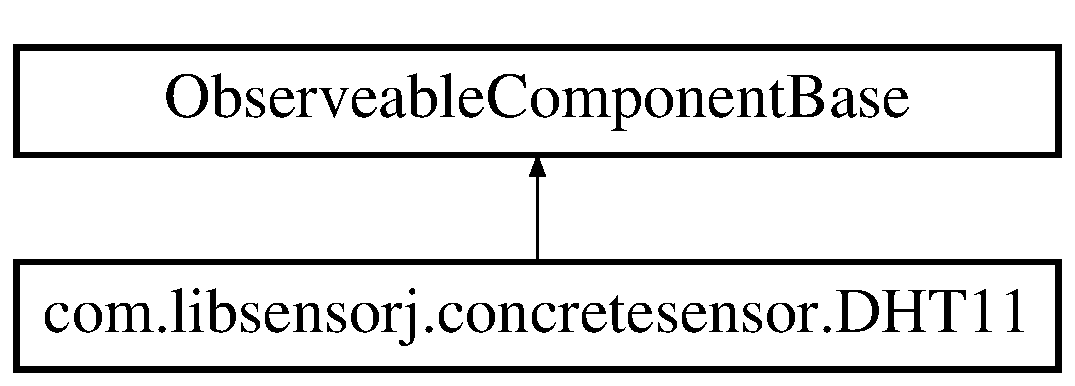
\includegraphics[height=2.000000cm]{classcom_1_1libsensorj_1_1concretesensor_1_1DHT11}
\end{center}
\end{figure}
\subsection*{Public Member Functions}
\begin{DoxyCompactItemize}
\item 
\hyperlink{classcom_1_1libsensorj_1_1concretesensor_1_1DHT11_a6dee6dabad63a5b8f8ba35f1279703c2}{D\+H\+T11} ()
\item 
\hyperlink{classcom_1_1libsensorj_1_1concretesensor_1_1DHT11_a6b867144169aa951ddbd09fc9ec5f6e5}{D\+H\+T11} (int pin)
\item 
double \hyperlink{classcom_1_1libsensorj_1_1concretesensor_1_1DHT11_a84f4c759756e582eb0e3d12675525c87}{read\+Value} ()
\item 
synchronized double \hyperlink{classcom_1_1libsensorj_1_1concretesensor_1_1DHT11_a4c88c53cbcacce861433ea2f03dd08f0}{get\+Temperature\+In\+Celsius} ()
\item 
synchronized double \hyperlink{classcom_1_1libsensorj_1_1concretesensor_1_1DHT11_a21bd2e0675b083a83610584d199c268b}{get\+Temperature\+In\+Fahrenheit} ()
\item 
synchronized double \hyperlink{classcom_1_1libsensorj_1_1concretesensor_1_1DHT11_ab2263c3d3e8deb1c1389fdb9c642b5ee}{get\+Temperature\+In\+Kelvin} ()
\end{DoxyCompactItemize}
\subsection*{Private Member Functions}
\begin{DoxyCompactItemize}
\item 
double \hyperlink{classcom_1_1libsensorj_1_1concretesensor_1_1DHT11_a1d452b9a4f3ff98d35cc425aee062bd4}{get\+Temperature} (Temperature\+Scale from)
\item 
boolean \hyperlink{classcom_1_1libsensorj_1_1concretesensor_1_1DHT11_a46fc1af81db68410209e81e5376428a9}{check\+Parity} ()
\end{DoxyCompactItemize}
\subsection*{Private Attributes}
\begin{DoxyCompactItemize}
\item 
int\mbox{[}$\,$\mbox{]} \hyperlink{classcom_1_1libsensorj_1_1concretesensor_1_1DHT11_a0d73b9b918bec661a7333f1f63e00d08}{dht11\+\_\+dat} = \{ 0, 0, 0, 0, 0 \}
\item 
Gpio\+Pin\+Digital\+Multipurpose \hyperlink{classcom_1_1libsensorj_1_1concretesensor_1_1DHT11_a816e6c7ffc2d313077cc5df4b2252b41}{dht11\+Pin}
\end{DoxyCompactItemize}
\subsection*{Static Private Attributes}
\begin{DoxyCompactItemize}
\item 
static final Pin \hyperlink{classcom_1_1libsensorj_1_1concretesensor_1_1DHT11_a90e62e8cc61299199eb1fa06bd441a9e}{D\+E\+F\+A\+U\+L\+T\+\_\+\+P\+I\+N} = Raspi\+Pin.\+G\+P\+I\+O\+\_\+04
\item 
static final int \hyperlink{classcom_1_1libsensorj_1_1concretesensor_1_1DHT11_ad986e37718b89038ff2702c80a2bb320}{M\+A\+X\+T\+I\+M\+I\+N\+G\+S} = 85
\item 
static final Logger \hyperlink{classcom_1_1libsensorj_1_1concretesensor_1_1DHT11_ad5b8d7e0ad34e4f3b28c081f259d1928}{L\+O\+G\+G\+E\+R}
\end{DoxyCompactItemize}


\subsection{Detailed Description}
The Class \hyperlink{classcom_1_1libsensorj_1_1concretesensor_1_1DHT11}{D\+H\+T11}. 

\subsection{Constructor \& Destructor Documentation}
\hypertarget{classcom_1_1libsensorj_1_1concretesensor_1_1DHT11_a6dee6dabad63a5b8f8ba35f1279703c2}{}\index{com\+::libsensorj\+::concretesensor\+::\+D\+H\+T11@{com\+::libsensorj\+::concretesensor\+::\+D\+H\+T11}!D\+H\+T11@{D\+H\+T11}}
\index{D\+H\+T11@{D\+H\+T11}!com\+::libsensorj\+::concretesensor\+::\+D\+H\+T11@{com\+::libsensorj\+::concretesensor\+::\+D\+H\+T11}}
\subsubsection[{D\+H\+T11}]{\setlength{\rightskip}{0pt plus 5cm}com.\+libsensorj.\+concretesensor.\+D\+H\+T11.\+D\+H\+T11 (
\begin{DoxyParamCaption}
{}
\end{DoxyParamCaption}
)}\label{classcom_1_1libsensorj_1_1concretesensor_1_1DHT11_a6dee6dabad63a5b8f8ba35f1279703c2}
Instantiates a new D\+Ht11. \hypertarget{classcom_1_1libsensorj_1_1concretesensor_1_1DHT11_a6b867144169aa951ddbd09fc9ec5f6e5}{}\index{com\+::libsensorj\+::concretesensor\+::\+D\+H\+T11@{com\+::libsensorj\+::concretesensor\+::\+D\+H\+T11}!D\+H\+T11@{D\+H\+T11}}
\index{D\+H\+T11@{D\+H\+T11}!com\+::libsensorj\+::concretesensor\+::\+D\+H\+T11@{com\+::libsensorj\+::concretesensor\+::\+D\+H\+T11}}
\subsubsection[{D\+H\+T11}]{\setlength{\rightskip}{0pt plus 5cm}com.\+libsensorj.\+concretesensor.\+D\+H\+T11.\+D\+H\+T11 (
\begin{DoxyParamCaption}
\item[{int}]{pin}
\end{DoxyParamCaption}
)}\label{classcom_1_1libsensorj_1_1concretesensor_1_1DHT11_a6b867144169aa951ddbd09fc9ec5f6e5}
Instantiates a new D\+Ht11.


\begin{DoxyParams}{Parameters}
{\em pin} & the pin \\
\hline
\end{DoxyParams}


\subsection{Member Function Documentation}
\hypertarget{classcom_1_1libsensorj_1_1concretesensor_1_1DHT11_a46fc1af81db68410209e81e5376428a9}{}\index{com\+::libsensorj\+::concretesensor\+::\+D\+H\+T11@{com\+::libsensorj\+::concretesensor\+::\+D\+H\+T11}!check\+Parity@{check\+Parity}}
\index{check\+Parity@{check\+Parity}!com\+::libsensorj\+::concretesensor\+::\+D\+H\+T11@{com\+::libsensorj\+::concretesensor\+::\+D\+H\+T11}}
\subsubsection[{check\+Parity}]{\setlength{\rightskip}{0pt plus 5cm}boolean com.\+libsensorj.\+concretesensor.\+D\+H\+T11.\+check\+Parity (
\begin{DoxyParamCaption}
{}
\end{DoxyParamCaption}
)\hspace{0.3cm}{\ttfamily [private]}}\label{classcom_1_1libsensorj_1_1concretesensor_1_1DHT11_a46fc1af81db68410209e81e5376428a9}
Check parity.

\begin{DoxyReturn}{Returns}
true, if successful 
\end{DoxyReturn}
\hypertarget{classcom_1_1libsensorj_1_1concretesensor_1_1DHT11_a1d452b9a4f3ff98d35cc425aee062bd4}{}\index{com\+::libsensorj\+::concretesensor\+::\+D\+H\+T11@{com\+::libsensorj\+::concretesensor\+::\+D\+H\+T11}!get\+Temperature@{get\+Temperature}}
\index{get\+Temperature@{get\+Temperature}!com\+::libsensorj\+::concretesensor\+::\+D\+H\+T11@{com\+::libsensorj\+::concretesensor\+::\+D\+H\+T11}}
\subsubsection[{get\+Temperature}]{\setlength{\rightskip}{0pt plus 5cm}double com.\+libsensorj.\+concretesensor.\+D\+H\+T11.\+get\+Temperature (
\begin{DoxyParamCaption}
\item[{Temperature\+Scale}]{from}
\end{DoxyParamCaption}
)\hspace{0.3cm}{\ttfamily [private]}}\label{classcom_1_1libsensorj_1_1concretesensor_1_1DHT11_a1d452b9a4f3ff98d35cc425aee062bd4}
Gets the temperature.


\begin{DoxyParams}{Parameters}
{\em from} & the Temperature\+Scale \\
\hline
\end{DoxyParams}
\begin{DoxyReturn}{Returns}
the temperature 
\end{DoxyReturn}
\hypertarget{classcom_1_1libsensorj_1_1concretesensor_1_1DHT11_a4c88c53cbcacce861433ea2f03dd08f0}{}\index{com\+::libsensorj\+::concretesensor\+::\+D\+H\+T11@{com\+::libsensorj\+::concretesensor\+::\+D\+H\+T11}!get\+Temperature\+In\+Celsius@{get\+Temperature\+In\+Celsius}}
\index{get\+Temperature\+In\+Celsius@{get\+Temperature\+In\+Celsius}!com\+::libsensorj\+::concretesensor\+::\+D\+H\+T11@{com\+::libsensorj\+::concretesensor\+::\+D\+H\+T11}}
\subsubsection[{get\+Temperature\+In\+Celsius}]{\setlength{\rightskip}{0pt plus 5cm}synchronized double com.\+libsensorj.\+concretesensor.\+D\+H\+T11.\+get\+Temperature\+In\+Celsius (
\begin{DoxyParamCaption}
{}
\end{DoxyParamCaption}
)}\label{classcom_1_1libsensorj_1_1concretesensor_1_1DHT11_a4c88c53cbcacce861433ea2f03dd08f0}
Gets the temperature in celsius.

\begin{DoxyReturn}{Returns}
the temperature in celsius 
\end{DoxyReturn}
\hypertarget{classcom_1_1libsensorj_1_1concretesensor_1_1DHT11_a21bd2e0675b083a83610584d199c268b}{}\index{com\+::libsensorj\+::concretesensor\+::\+D\+H\+T11@{com\+::libsensorj\+::concretesensor\+::\+D\+H\+T11}!get\+Temperature\+In\+Fahrenheit@{get\+Temperature\+In\+Fahrenheit}}
\index{get\+Temperature\+In\+Fahrenheit@{get\+Temperature\+In\+Fahrenheit}!com\+::libsensorj\+::concretesensor\+::\+D\+H\+T11@{com\+::libsensorj\+::concretesensor\+::\+D\+H\+T11}}
\subsubsection[{get\+Temperature\+In\+Fahrenheit}]{\setlength{\rightskip}{0pt plus 5cm}synchronized double com.\+libsensorj.\+concretesensor.\+D\+H\+T11.\+get\+Temperature\+In\+Fahrenheit (
\begin{DoxyParamCaption}
{}
\end{DoxyParamCaption}
)}\label{classcom_1_1libsensorj_1_1concretesensor_1_1DHT11_a21bd2e0675b083a83610584d199c268b}
Gets the temperature in fahrenheit.

\begin{DoxyReturn}{Returns}
the temperature in fahrenheit 
\end{DoxyReturn}
\hypertarget{classcom_1_1libsensorj_1_1concretesensor_1_1DHT11_ab2263c3d3e8deb1c1389fdb9c642b5ee}{}\index{com\+::libsensorj\+::concretesensor\+::\+D\+H\+T11@{com\+::libsensorj\+::concretesensor\+::\+D\+H\+T11}!get\+Temperature\+In\+Kelvin@{get\+Temperature\+In\+Kelvin}}
\index{get\+Temperature\+In\+Kelvin@{get\+Temperature\+In\+Kelvin}!com\+::libsensorj\+::concretesensor\+::\+D\+H\+T11@{com\+::libsensorj\+::concretesensor\+::\+D\+H\+T11}}
\subsubsection[{get\+Temperature\+In\+Kelvin}]{\setlength{\rightskip}{0pt plus 5cm}synchronized double com.\+libsensorj.\+concretesensor.\+D\+H\+T11.\+get\+Temperature\+In\+Kelvin (
\begin{DoxyParamCaption}
{}
\end{DoxyParamCaption}
)}\label{classcom_1_1libsensorj_1_1concretesensor_1_1DHT11_ab2263c3d3e8deb1c1389fdb9c642b5ee}
Gets the temperature in kelvin.

\begin{DoxyReturn}{Returns}
the temperature in kelvin 
\end{DoxyReturn}
\hypertarget{classcom_1_1libsensorj_1_1concretesensor_1_1DHT11_a84f4c759756e582eb0e3d12675525c87}{}\index{com\+::libsensorj\+::concretesensor\+::\+D\+H\+T11@{com\+::libsensorj\+::concretesensor\+::\+D\+H\+T11}!read\+Value@{read\+Value}}
\index{read\+Value@{read\+Value}!com\+::libsensorj\+::concretesensor\+::\+D\+H\+T11@{com\+::libsensorj\+::concretesensor\+::\+D\+H\+T11}}
\subsubsection[{read\+Value}]{\setlength{\rightskip}{0pt plus 5cm}double com.\+libsensorj.\+concretesensor.\+D\+H\+T11.\+read\+Value (
\begin{DoxyParamCaption}
{}
\end{DoxyParamCaption}
)}\label{classcom_1_1libsensorj_1_1concretesensor_1_1DHT11_a84f4c759756e582eb0e3d12675525c87}
Read value.

\begin{DoxyReturn}{Returns}
the value readed 
\end{DoxyReturn}


\subsection{Member Data Documentation}
\hypertarget{classcom_1_1libsensorj_1_1concretesensor_1_1DHT11_a90e62e8cc61299199eb1fa06bd441a9e}{}\index{com\+::libsensorj\+::concretesensor\+::\+D\+H\+T11@{com\+::libsensorj\+::concretesensor\+::\+D\+H\+T11}!D\+E\+F\+A\+U\+L\+T\+\_\+\+P\+I\+N@{D\+E\+F\+A\+U\+L\+T\+\_\+\+P\+I\+N}}
\index{D\+E\+F\+A\+U\+L\+T\+\_\+\+P\+I\+N@{D\+E\+F\+A\+U\+L\+T\+\_\+\+P\+I\+N}!com\+::libsensorj\+::concretesensor\+::\+D\+H\+T11@{com\+::libsensorj\+::concretesensor\+::\+D\+H\+T11}}
\subsubsection[{D\+E\+F\+A\+U\+L\+T\+\_\+\+P\+I\+N}]{\setlength{\rightskip}{0pt plus 5cm}final Pin com.\+libsensorj.\+concretesensor.\+D\+H\+T11.\+D\+E\+F\+A\+U\+L\+T\+\_\+\+P\+I\+N = Raspi\+Pin.\+G\+P\+I\+O\+\_\+04\hspace{0.3cm}{\ttfamily [static]}, {\ttfamily [private]}}\label{classcom_1_1libsensorj_1_1concretesensor_1_1DHT11_a90e62e8cc61299199eb1fa06bd441a9e}
The Constant D\+E\+F\+A\+U\+L\+T\+\_\+\+P\+I\+N. \hypertarget{classcom_1_1libsensorj_1_1concretesensor_1_1DHT11_a0d73b9b918bec661a7333f1f63e00d08}{}\index{com\+::libsensorj\+::concretesensor\+::\+D\+H\+T11@{com\+::libsensorj\+::concretesensor\+::\+D\+H\+T11}!dht11\+\_\+dat@{dht11\+\_\+dat}}
\index{dht11\+\_\+dat@{dht11\+\_\+dat}!com\+::libsensorj\+::concretesensor\+::\+D\+H\+T11@{com\+::libsensorj\+::concretesensor\+::\+D\+H\+T11}}
\subsubsection[{dht11\+\_\+dat}]{\setlength{\rightskip}{0pt plus 5cm}int \mbox{[}$\,$\mbox{]} com.\+libsensorj.\+concretesensor.\+D\+H\+T11.\+dht11\+\_\+dat = \{ 0, 0, 0, 0, 0 \}\hspace{0.3cm}{\ttfamily [private]}}\label{classcom_1_1libsensorj_1_1concretesensor_1_1DHT11_a0d73b9b918bec661a7333f1f63e00d08}
The dht11\+\_\+dat. \hypertarget{classcom_1_1libsensorj_1_1concretesensor_1_1DHT11_a816e6c7ffc2d313077cc5df4b2252b41}{}\index{com\+::libsensorj\+::concretesensor\+::\+D\+H\+T11@{com\+::libsensorj\+::concretesensor\+::\+D\+H\+T11}!dht11\+Pin@{dht11\+Pin}}
\index{dht11\+Pin@{dht11\+Pin}!com\+::libsensorj\+::concretesensor\+::\+D\+H\+T11@{com\+::libsensorj\+::concretesensor\+::\+D\+H\+T11}}
\subsubsection[{dht11\+Pin}]{\setlength{\rightskip}{0pt plus 5cm}Gpio\+Pin\+Digital\+Multipurpose com.\+libsensorj.\+concretesensor.\+D\+H\+T11.\+dht11\+Pin\hspace{0.3cm}{\ttfamily [private]}}\label{classcom_1_1libsensorj_1_1concretesensor_1_1DHT11_a816e6c7ffc2d313077cc5df4b2252b41}
The dht11 pin. \hypertarget{classcom_1_1libsensorj_1_1concretesensor_1_1DHT11_ad5b8d7e0ad34e4f3b28c081f259d1928}{}\index{com\+::libsensorj\+::concretesensor\+::\+D\+H\+T11@{com\+::libsensorj\+::concretesensor\+::\+D\+H\+T11}!L\+O\+G\+G\+E\+R@{L\+O\+G\+G\+E\+R}}
\index{L\+O\+G\+G\+E\+R@{L\+O\+G\+G\+E\+R}!com\+::libsensorj\+::concretesensor\+::\+D\+H\+T11@{com\+::libsensorj\+::concretesensor\+::\+D\+H\+T11}}
\subsubsection[{L\+O\+G\+G\+E\+R}]{\setlength{\rightskip}{0pt plus 5cm}final Logger com.\+libsensorj.\+concretesensor.\+D\+H\+T11.\+L\+O\+G\+G\+E\+R\hspace{0.3cm}{\ttfamily [static]}, {\ttfamily [private]}}\label{classcom_1_1libsensorj_1_1concretesensor_1_1DHT11_ad5b8d7e0ad34e4f3b28c081f259d1928}
{\bfseries Initial value\+:}
\begin{DoxyCode}
= LogManager.getLogger(\hyperlink{classcom_1_1libsensorj_1_1concretesensor_1_1DHT11_a6dee6dabad63a5b8f8ba35f1279703c2}{DHT11}.class
            .getName())
\end{DoxyCode}
The Constant L\+O\+G\+G\+E\+R. \hypertarget{classcom_1_1libsensorj_1_1concretesensor_1_1DHT11_ad986e37718b89038ff2702c80a2bb320}{}\index{com\+::libsensorj\+::concretesensor\+::\+D\+H\+T11@{com\+::libsensorj\+::concretesensor\+::\+D\+H\+T11}!M\+A\+X\+T\+I\+M\+I\+N\+G\+S@{M\+A\+X\+T\+I\+M\+I\+N\+G\+S}}
\index{M\+A\+X\+T\+I\+M\+I\+N\+G\+S@{M\+A\+X\+T\+I\+M\+I\+N\+G\+S}!com\+::libsensorj\+::concretesensor\+::\+D\+H\+T11@{com\+::libsensorj\+::concretesensor\+::\+D\+H\+T11}}
\subsubsection[{M\+A\+X\+T\+I\+M\+I\+N\+G\+S}]{\setlength{\rightskip}{0pt plus 5cm}final int com.\+libsensorj.\+concretesensor.\+D\+H\+T11.\+M\+A\+X\+T\+I\+M\+I\+N\+G\+S = 85\hspace{0.3cm}{\ttfamily [static]}, {\ttfamily [private]}}\label{classcom_1_1libsensorj_1_1concretesensor_1_1DHT11_ad986e37718b89038ff2702c80a2bb320}
The Constant M\+A\+X\+T\+I\+M\+I\+N\+G\+S. 

The documentation for this class was generated from the following file\+:\begin{DoxyCompactItemize}
\item 
main/java/com/libsensorj/concretesensor/\hyperlink{DHT11_8java}{D\+H\+T11.\+java}\end{DoxyCompactItemize}

\hypertarget{classcom_1_1libsensorj_1_1concretesensor_1_1DHT11Humidity}{}\section{com.\+libsensorj.\+concretesensor.\+D\+H\+T11\+Humidity Class Reference}
\label{classcom_1_1libsensorj_1_1concretesensor_1_1DHT11Humidity}\index{com.\+libsensorj.\+concretesensor.\+D\+H\+T11\+Humidity@{com.\+libsensorj.\+concretesensor.\+D\+H\+T11\+Humidity}}
Inheritance diagram for com.\+libsensorj.\+concretesensor.\+D\+H\+T11\+Humidity\+:\begin{figure}[H]
\begin{center}
\leavevmode
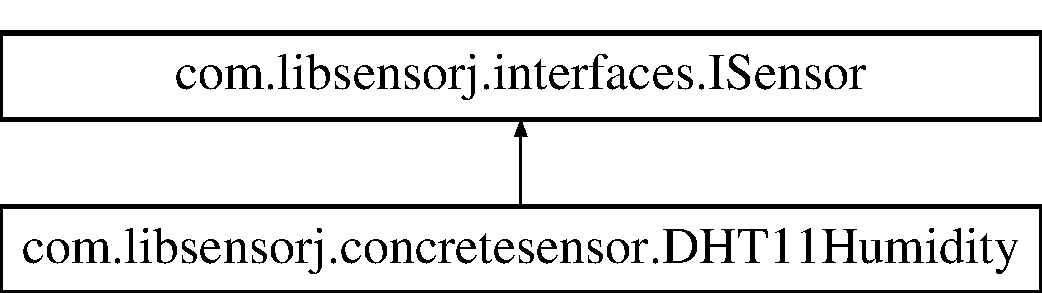
\includegraphics[height=2.000000cm]{classcom_1_1libsensorj_1_1concretesensor_1_1DHT11Humidity}
\end{center}
\end{figure}
\subsection*{Public Member Functions}
\begin{DoxyCompactItemize}
\item 
void \hyperlink{classcom_1_1libsensorj_1_1concretesensor_1_1DHT11Humidity_a2355dc003abad8d519440e9f6871c422}{get\+Instance} ()
\end{DoxyCompactItemize}
\subsection*{Static Private Attributes}
\begin{DoxyCompactItemize}
\item 
static final Logger \hyperlink{classcom_1_1libsensorj_1_1concretesensor_1_1DHT11Humidity_a80655575ba16db014b7a1a797e030eae}{L\+O\+G\+G\+E\+R}
\end{DoxyCompactItemize}


\subsection{Detailed Description}
The Class \hyperlink{classcom_1_1libsensorj_1_1concretesensor_1_1DHT11Humidity}{D\+H\+T11\+Humidity}. 

\subsection{Member Function Documentation}
\hypertarget{classcom_1_1libsensorj_1_1concretesensor_1_1DHT11Humidity_a2355dc003abad8d519440e9f6871c422}{}\index{com\+::libsensorj\+::concretesensor\+::\+D\+H\+T11\+Humidity@{com\+::libsensorj\+::concretesensor\+::\+D\+H\+T11\+Humidity}!get\+Instance@{get\+Instance}}
\index{get\+Instance@{get\+Instance}!com\+::libsensorj\+::concretesensor\+::\+D\+H\+T11\+Humidity@{com\+::libsensorj\+::concretesensor\+::\+D\+H\+T11\+Humidity}}
\subsubsection[{get\+Instance}]{\setlength{\rightskip}{0pt plus 5cm}void com.\+libsensorj.\+concretesensor.\+D\+H\+T11\+Humidity.\+get\+Instance (
\begin{DoxyParamCaption}
{}
\end{DoxyParamCaption}
)}\label{classcom_1_1libsensorj_1_1concretesensor_1_1DHT11Humidity_a2355dc003abad8d519440e9f6871c422}
Gets the single instance of I\+Sensor.

\begin{DoxyReturn}{Returns}
single instance of I\+Sensor 
\end{DoxyReturn}


Implements \hyperlink{interfacecom_1_1libsensorj_1_1interfaces_1_1ISensor_a3c3db93a33adecde81a528651790f75e}{com.\+libsensorj.\+interfaces.\+I\+Sensor}.



\subsection{Member Data Documentation}
\hypertarget{classcom_1_1libsensorj_1_1concretesensor_1_1DHT11Humidity_a80655575ba16db014b7a1a797e030eae}{}\index{com\+::libsensorj\+::concretesensor\+::\+D\+H\+T11\+Humidity@{com\+::libsensorj\+::concretesensor\+::\+D\+H\+T11\+Humidity}!L\+O\+G\+G\+E\+R@{L\+O\+G\+G\+E\+R}}
\index{L\+O\+G\+G\+E\+R@{L\+O\+G\+G\+E\+R}!com\+::libsensorj\+::concretesensor\+::\+D\+H\+T11\+Humidity@{com\+::libsensorj\+::concretesensor\+::\+D\+H\+T11\+Humidity}}
\subsubsection[{L\+O\+G\+G\+E\+R}]{\setlength{\rightskip}{0pt plus 5cm}final Logger com.\+libsensorj.\+concretesensor.\+D\+H\+T11\+Humidity.\+L\+O\+G\+G\+E\+R\hspace{0.3cm}{\ttfamily [static]}, {\ttfamily [private]}}\label{classcom_1_1libsensorj_1_1concretesensor_1_1DHT11Humidity_a80655575ba16db014b7a1a797e030eae}
{\bfseries Initial value\+:}
\begin{DoxyCode}
= LogManager
            .getLogger(DHT11Humidity.class.getName())
\end{DoxyCode}
The Constant L\+O\+G\+G\+E\+R. 

The documentation for this class was generated from the following file\+:\begin{DoxyCompactItemize}
\item 
main/java/com/libsensorj/concretesensor/\hyperlink{DHT11Humidity_8java}{D\+H\+T11\+Humidity.\+java}\end{DoxyCompactItemize}

\hypertarget{classcom_1_1libsensorj_1_1examples_1_1DHT11HumidityExample}{}\section{com.\+libsensorj.\+examples.\+D\+H\+T11\+Humidity\+Example Class Reference}
\label{classcom_1_1libsensorj_1_1examples_1_1DHT11HumidityExample}\index{com.\+libsensorj.\+examples.\+D\+H\+T11\+Humidity\+Example@{com.\+libsensorj.\+examples.\+D\+H\+T11\+Humidity\+Example}}
\subsection*{Static Public Member Functions}
\begin{DoxyCompactItemize}
\item 
static void \hyperlink{classcom_1_1libsensorj_1_1examples_1_1DHT11HumidityExample_ad906ca82a6b80ab356f098b5705b2626}{main} (String\mbox{[}$\,$\mbox{]} args)
\end{DoxyCompactItemize}
\subsection*{Static Private Attributes}
\begin{DoxyCompactItemize}
\item 
static \hyperlink{interfacecom_1_1libsensorj_1_1interfaces_1_1ISensor}{I\+Sensor} \hyperlink{classcom_1_1libsensorj_1_1examples_1_1DHT11HumidityExample_a4e50eabfe642f347fcf1b39198da5739}{dht11}
\item 
static final Logger \hyperlink{classcom_1_1libsensorj_1_1examples_1_1DHT11HumidityExample_aee9ba7d87ffaf4d9571628bf3017ed61}{L\+O\+G\+G\+E\+R}
\end{DoxyCompactItemize}


\subsection{Detailed Description}
The Class \hyperlink{classcom_1_1libsensorj_1_1examples_1_1DHT11HumidityExample}{D\+H\+T11\+Humidity\+Example}. 

\subsection{Member Function Documentation}
\hypertarget{classcom_1_1libsensorj_1_1examples_1_1DHT11HumidityExample_ad906ca82a6b80ab356f098b5705b2626}{}\index{com\+::libsensorj\+::examples\+::\+D\+H\+T11\+Humidity\+Example@{com\+::libsensorj\+::examples\+::\+D\+H\+T11\+Humidity\+Example}!main@{main}}
\index{main@{main}!com\+::libsensorj\+::examples\+::\+D\+H\+T11\+Humidity\+Example@{com\+::libsensorj\+::examples\+::\+D\+H\+T11\+Humidity\+Example}}
\subsubsection[{main}]{\setlength{\rightskip}{0pt plus 5cm}static void com.\+libsensorj.\+examples.\+D\+H\+T11\+Humidity\+Example.\+main (
\begin{DoxyParamCaption}
\item[{String\mbox{[}$\,$\mbox{]}}]{args}
\end{DoxyParamCaption}
)\hspace{0.3cm}{\ttfamily [static]}}\label{classcom_1_1libsensorj_1_1examples_1_1DHT11HumidityExample_ad906ca82a6b80ab356f098b5705b2626}
The main method.


\begin{DoxyParams}{Parameters}
{\em args} & the arguments \\
\hline
\end{DoxyParams}


\subsection{Member Data Documentation}
\hypertarget{classcom_1_1libsensorj_1_1examples_1_1DHT11HumidityExample_a4e50eabfe642f347fcf1b39198da5739}{}\index{com\+::libsensorj\+::examples\+::\+D\+H\+T11\+Humidity\+Example@{com\+::libsensorj\+::examples\+::\+D\+H\+T11\+Humidity\+Example}!dht11@{dht11}}
\index{dht11@{dht11}!com\+::libsensorj\+::examples\+::\+D\+H\+T11\+Humidity\+Example@{com\+::libsensorj\+::examples\+::\+D\+H\+T11\+Humidity\+Example}}
\subsubsection[{dht11}]{\setlength{\rightskip}{0pt plus 5cm}{\bf I\+Sensor} com.\+libsensorj.\+examples.\+D\+H\+T11\+Humidity\+Example.\+dht11\hspace{0.3cm}{\ttfamily [static]}, {\ttfamily [private]}}\label{classcom_1_1libsensorj_1_1examples_1_1DHT11HumidityExample_a4e50eabfe642f347fcf1b39198da5739}
The Isensor dht11. \hypertarget{classcom_1_1libsensorj_1_1examples_1_1DHT11HumidityExample_aee9ba7d87ffaf4d9571628bf3017ed61}{}\index{com\+::libsensorj\+::examples\+::\+D\+H\+T11\+Humidity\+Example@{com\+::libsensorj\+::examples\+::\+D\+H\+T11\+Humidity\+Example}!L\+O\+G\+G\+E\+R@{L\+O\+G\+G\+E\+R}}
\index{L\+O\+G\+G\+E\+R@{L\+O\+G\+G\+E\+R}!com\+::libsensorj\+::examples\+::\+D\+H\+T11\+Humidity\+Example@{com\+::libsensorj\+::examples\+::\+D\+H\+T11\+Humidity\+Example}}
\subsubsection[{L\+O\+G\+G\+E\+R}]{\setlength{\rightskip}{0pt plus 5cm}final Logger com.\+libsensorj.\+examples.\+D\+H\+T11\+Humidity\+Example.\+L\+O\+G\+G\+E\+R\hspace{0.3cm}{\ttfamily [static]}, {\ttfamily [private]}}\label{classcom_1_1libsensorj_1_1examples_1_1DHT11HumidityExample_aee9ba7d87ffaf4d9571628bf3017ed61}
{\bfseries Initial value\+:}
\begin{DoxyCode}
= LogManager
            .getLogger(DHT11TemperatureExample.class.getName())
\end{DoxyCode}
The Constant L\+O\+G\+G\+E\+R. 

The documentation for this class was generated from the following file\+:\begin{DoxyCompactItemize}
\item 
main/java/com/libsensorj/examples/\hyperlink{DHT11HumidityExample_8java}{D\+H\+T11\+Humidity\+Example.\+java}\end{DoxyCompactItemize}

\hypertarget{classcom_1_1libsensorj_1_1concretesensor_1_1test_1_1DHT11HumidityTests}{}\section{com.\+libsensorj.\+concretesensor.\+test.\+D\+H\+T11\+Humidity\+Tests Class Reference}
\label{classcom_1_1libsensorj_1_1concretesensor_1_1test_1_1DHT11HumidityTests}\index{com.\+libsensorj.\+concretesensor.\+test.\+D\+H\+T11\+Humidity\+Tests@{com.\+libsensorj.\+concretesensor.\+test.\+D\+H\+T11\+Humidity\+Tests}}
\subsection*{Public Member Functions}
\begin{DoxyCompactItemize}
\item 
void \hyperlink{classcom_1_1libsensorj_1_1concretesensor_1_1test_1_1DHT11HumidityTests_aa430d9d41ff4c44bc96e26c56b766764}{test\+Pin\+Provisioned} ()
\item 
void \hyperlink{classcom_1_1libsensorj_1_1concretesensor_1_1test_1_1DHT11HumidityTests_a04e45fe8c38426fc82c1dceee5d87b71}{test\+Get\+Humidity} ()
\end{DoxyCompactItemize}
\subsection*{Static Public Member Functions}
\begin{DoxyCompactItemize}
\item 
static void \hyperlink{classcom_1_1libsensorj_1_1concretesensor_1_1test_1_1DHT11HumidityTests_aef0e68198d00aff7b82f1e71cf91f12d}{setup} ()
\end{DoxyCompactItemize}
\subsection*{Static Private Attributes}
\begin{DoxyCompactItemize}
\item 
static Gpio\+Controller \hyperlink{classcom_1_1libsensorj_1_1concretesensor_1_1test_1_1DHT11HumidityTests_a3631933a16a10839ab88bc36bc068126}{gpio}
\item 
static Gpio\+Pin\+Digital\+Input \hyperlink{classcom_1_1libsensorj_1_1concretesensor_1_1test_1_1DHT11HumidityTests_a9c5ef0f8073d54cec2b80c9b54aef2d1}{pin}
\item 
static Pin\+State \hyperlink{classcom_1_1libsensorj_1_1concretesensor_1_1test_1_1DHT11HumidityTests_aa4907b3b4ddbc118b0bb5a8571d17202}{pin\+Monitored\+State}
\item 
static final String \hyperlink{classcom_1_1libsensorj_1_1concretesensor_1_1test_1_1DHT11HumidityTests_a17f48d78c744c6773af54f613a7c670e}{D\+A\+T\+A\+\_\+\+R\+E\+A\+D\+E\+D} = \char`\"{}Using \hyperlink{classcom_1_1libsensorj_1_1concretesensor_1_1test_1_1DHT11HumidityTests_a9c5ef0f8073d54cec2b80c9b54aef2d1}{pin} \#4\+Data (40)\+: 0x32 0x0 0x1d 0x0 0x4f\+Temp = 29 $\ast$\+C, Hum = 50 \%\char`\"{}
\item 
static final String \hyperlink{classcom_1_1libsensorj_1_1concretesensor_1_1test_1_1DHT11HumidityTests_a990e9ce8e27fda4153926133ef67cb4f}{R\+E\+A\+D\+V\+A\+L\+U\+E\+S\+\_\+\+M\+E\+T\+H\+O\+D} = \char`\"{}read\+Values\char`\"{}
\item 
static final Logger \hyperlink{classcom_1_1libsensorj_1_1concretesensor_1_1test_1_1DHT11HumidityTests_a6423bd32a25b5e850b3b36abdc9bc31a}{L\+O\+G\+G\+E\+R}
\end{DoxyCompactItemize}


\subsection{Detailed Description}
The Class \hyperlink{classcom_1_1libsensorj_1_1concretesensor_1_1test_1_1DHT11TemperatureTests}{D\+H\+T11\+Temperature\+Tests}. 

\subsection{Member Function Documentation}
\hypertarget{classcom_1_1libsensorj_1_1concretesensor_1_1test_1_1DHT11HumidityTests_aef0e68198d00aff7b82f1e71cf91f12d}{}\index{com\+::libsensorj\+::concretesensor\+::test\+::\+D\+H\+T11\+Humidity\+Tests@{com\+::libsensorj\+::concretesensor\+::test\+::\+D\+H\+T11\+Humidity\+Tests}!setup@{setup}}
\index{setup@{setup}!com\+::libsensorj\+::concretesensor\+::test\+::\+D\+H\+T11\+Humidity\+Tests@{com\+::libsensorj\+::concretesensor\+::test\+::\+D\+H\+T11\+Humidity\+Tests}}
\subsubsection[{setup}]{\setlength{\rightskip}{0pt plus 5cm}static void com.\+libsensorj.\+concretesensor.\+test.\+D\+H\+T11\+Humidity\+Tests.\+setup (
\begin{DoxyParamCaption}
{}
\end{DoxyParamCaption}
)\hspace{0.3cm}{\ttfamily [static]}}\label{classcom_1_1libsensorj_1_1concretesensor_1_1test_1_1DHT11HumidityTests_aef0e68198d00aff7b82f1e71cf91f12d}
Setup. \hypertarget{classcom_1_1libsensorj_1_1concretesensor_1_1test_1_1DHT11HumidityTests_a04e45fe8c38426fc82c1dceee5d87b71}{}\index{com\+::libsensorj\+::concretesensor\+::test\+::\+D\+H\+T11\+Humidity\+Tests@{com\+::libsensorj\+::concretesensor\+::test\+::\+D\+H\+T11\+Humidity\+Tests}!test\+Get\+Humidity@{test\+Get\+Humidity}}
\index{test\+Get\+Humidity@{test\+Get\+Humidity}!com\+::libsensorj\+::concretesensor\+::test\+::\+D\+H\+T11\+Humidity\+Tests@{com\+::libsensorj\+::concretesensor\+::test\+::\+D\+H\+T11\+Humidity\+Tests}}
\subsubsection[{test\+Get\+Humidity}]{\setlength{\rightskip}{0pt plus 5cm}void com.\+libsensorj.\+concretesensor.\+test.\+D\+H\+T11\+Humidity\+Tests.\+test\+Get\+Humidity (
\begin{DoxyParamCaption}
{}
\end{DoxyParamCaption}
)}\label{classcom_1_1libsensorj_1_1concretesensor_1_1test_1_1DHT11HumidityTests_a04e45fe8c38426fc82c1dceee5d87b71}
Test Get\+Humidity. \hypertarget{classcom_1_1libsensorj_1_1concretesensor_1_1test_1_1DHT11HumidityTests_aa430d9d41ff4c44bc96e26c56b766764}{}\index{com\+::libsensorj\+::concretesensor\+::test\+::\+D\+H\+T11\+Humidity\+Tests@{com\+::libsensorj\+::concretesensor\+::test\+::\+D\+H\+T11\+Humidity\+Tests}!test\+Pin\+Provisioned@{test\+Pin\+Provisioned}}
\index{test\+Pin\+Provisioned@{test\+Pin\+Provisioned}!com\+::libsensorj\+::concretesensor\+::test\+::\+D\+H\+T11\+Humidity\+Tests@{com\+::libsensorj\+::concretesensor\+::test\+::\+D\+H\+T11\+Humidity\+Tests}}
\subsubsection[{test\+Pin\+Provisioned}]{\setlength{\rightskip}{0pt plus 5cm}void com.\+libsensorj.\+concretesensor.\+test.\+D\+H\+T11\+Humidity\+Tests.\+test\+Pin\+Provisioned (
\begin{DoxyParamCaption}
{}
\end{DoxyParamCaption}
)}\label{classcom_1_1libsensorj_1_1concretesensor_1_1test_1_1DHT11HumidityTests_aa430d9d41ff4c44bc96e26c56b766764}
Test pin provisioned. 

\subsection{Member Data Documentation}
\hypertarget{classcom_1_1libsensorj_1_1concretesensor_1_1test_1_1DHT11HumidityTests_a17f48d78c744c6773af54f613a7c670e}{}\index{com\+::libsensorj\+::concretesensor\+::test\+::\+D\+H\+T11\+Humidity\+Tests@{com\+::libsensorj\+::concretesensor\+::test\+::\+D\+H\+T11\+Humidity\+Tests}!D\+A\+T\+A\+\_\+\+R\+E\+A\+D\+E\+D@{D\+A\+T\+A\+\_\+\+R\+E\+A\+D\+E\+D}}
\index{D\+A\+T\+A\+\_\+\+R\+E\+A\+D\+E\+D@{D\+A\+T\+A\+\_\+\+R\+E\+A\+D\+E\+D}!com\+::libsensorj\+::concretesensor\+::test\+::\+D\+H\+T11\+Humidity\+Tests@{com\+::libsensorj\+::concretesensor\+::test\+::\+D\+H\+T11\+Humidity\+Tests}}
\subsubsection[{D\+A\+T\+A\+\_\+\+R\+E\+A\+D\+E\+D}]{\setlength{\rightskip}{0pt plus 5cm}final String com.\+libsensorj.\+concretesensor.\+test.\+D\+H\+T11\+Humidity\+Tests.\+D\+A\+T\+A\+\_\+\+R\+E\+A\+D\+E\+D = \char`\"{}Using {\bf pin} \#4\+Data (40)\+: 0x32 0x0 0x1d 0x0 0x4f\+Temp = 29 $\ast$\+C, Hum = 50 \%\char`\"{}\hspace{0.3cm}{\ttfamily [static]}, {\ttfamily [private]}}\label{classcom_1_1libsensorj_1_1concretesensor_1_1test_1_1DHT11HumidityTests_a17f48d78c744c6773af54f613a7c670e}
The Constant D\+A\+T\+A\+\_\+\+R\+E\+A\+D\+E\+D. \hypertarget{classcom_1_1libsensorj_1_1concretesensor_1_1test_1_1DHT11HumidityTests_a3631933a16a10839ab88bc36bc068126}{}\index{com\+::libsensorj\+::concretesensor\+::test\+::\+D\+H\+T11\+Humidity\+Tests@{com\+::libsensorj\+::concretesensor\+::test\+::\+D\+H\+T11\+Humidity\+Tests}!gpio@{gpio}}
\index{gpio@{gpio}!com\+::libsensorj\+::concretesensor\+::test\+::\+D\+H\+T11\+Humidity\+Tests@{com\+::libsensorj\+::concretesensor\+::test\+::\+D\+H\+T11\+Humidity\+Tests}}
\subsubsection[{gpio}]{\setlength{\rightskip}{0pt plus 5cm}Gpio\+Controller com.\+libsensorj.\+concretesensor.\+test.\+D\+H\+T11\+Humidity\+Tests.\+gpio\hspace{0.3cm}{\ttfamily [static]}, {\ttfamily [private]}}\label{classcom_1_1libsensorj_1_1concretesensor_1_1test_1_1DHT11HumidityTests_a3631933a16a10839ab88bc36bc068126}
The provider. The gpio. \hypertarget{classcom_1_1libsensorj_1_1concretesensor_1_1test_1_1DHT11HumidityTests_a6423bd32a25b5e850b3b36abdc9bc31a}{}\index{com\+::libsensorj\+::concretesensor\+::test\+::\+D\+H\+T11\+Humidity\+Tests@{com\+::libsensorj\+::concretesensor\+::test\+::\+D\+H\+T11\+Humidity\+Tests}!L\+O\+G\+G\+E\+R@{L\+O\+G\+G\+E\+R}}
\index{L\+O\+G\+G\+E\+R@{L\+O\+G\+G\+E\+R}!com\+::libsensorj\+::concretesensor\+::test\+::\+D\+H\+T11\+Humidity\+Tests@{com\+::libsensorj\+::concretesensor\+::test\+::\+D\+H\+T11\+Humidity\+Tests}}
\subsubsection[{L\+O\+G\+G\+E\+R}]{\setlength{\rightskip}{0pt plus 5cm}final Logger com.\+libsensorj.\+concretesensor.\+test.\+D\+H\+T11\+Humidity\+Tests.\+L\+O\+G\+G\+E\+R\hspace{0.3cm}{\ttfamily [static]}, {\ttfamily [private]}}\label{classcom_1_1libsensorj_1_1concretesensor_1_1test_1_1DHT11HumidityTests_a6423bd32a25b5e850b3b36abdc9bc31a}
{\bfseries Initial value\+:}
\begin{DoxyCode}
= LogManager
            .getLogger(DHT11TemperatureTests.class.getName())
\end{DoxyCode}
The Constant L\+O\+G\+G\+E\+R. \hypertarget{classcom_1_1libsensorj_1_1concretesensor_1_1test_1_1DHT11HumidityTests_a9c5ef0f8073d54cec2b80c9b54aef2d1}{}\index{com\+::libsensorj\+::concretesensor\+::test\+::\+D\+H\+T11\+Humidity\+Tests@{com\+::libsensorj\+::concretesensor\+::test\+::\+D\+H\+T11\+Humidity\+Tests}!pin@{pin}}
\index{pin@{pin}!com\+::libsensorj\+::concretesensor\+::test\+::\+D\+H\+T11\+Humidity\+Tests@{com\+::libsensorj\+::concretesensor\+::test\+::\+D\+H\+T11\+Humidity\+Tests}}
\subsubsection[{pin}]{\setlength{\rightskip}{0pt plus 5cm}Gpio\+Pin\+Digital\+Input com.\+libsensorj.\+concretesensor.\+test.\+D\+H\+T11\+Humidity\+Tests.\+pin\hspace{0.3cm}{\ttfamily [static]}, {\ttfamily [private]}}\label{classcom_1_1libsensorj_1_1concretesensor_1_1test_1_1DHT11HumidityTests_a9c5ef0f8073d54cec2b80c9b54aef2d1}
The pin. \hypertarget{classcom_1_1libsensorj_1_1concretesensor_1_1test_1_1DHT11HumidityTests_aa4907b3b4ddbc118b0bb5a8571d17202}{}\index{com\+::libsensorj\+::concretesensor\+::test\+::\+D\+H\+T11\+Humidity\+Tests@{com\+::libsensorj\+::concretesensor\+::test\+::\+D\+H\+T11\+Humidity\+Tests}!pin\+Monitored\+State@{pin\+Monitored\+State}}
\index{pin\+Monitored\+State@{pin\+Monitored\+State}!com\+::libsensorj\+::concretesensor\+::test\+::\+D\+H\+T11\+Humidity\+Tests@{com\+::libsensorj\+::concretesensor\+::test\+::\+D\+H\+T11\+Humidity\+Tests}}
\subsubsection[{pin\+Monitored\+State}]{\setlength{\rightskip}{0pt plus 5cm}Pin\+State com.\+libsensorj.\+concretesensor.\+test.\+D\+H\+T11\+Humidity\+Tests.\+pin\+Monitored\+State\hspace{0.3cm}{\ttfamily [static]}, {\ttfamily [private]}}\label{classcom_1_1libsensorj_1_1concretesensor_1_1test_1_1DHT11HumidityTests_aa4907b3b4ddbc118b0bb5a8571d17202}
The pin monitored state. \hypertarget{classcom_1_1libsensorj_1_1concretesensor_1_1test_1_1DHT11HumidityTests_a990e9ce8e27fda4153926133ef67cb4f}{}\index{com\+::libsensorj\+::concretesensor\+::test\+::\+D\+H\+T11\+Humidity\+Tests@{com\+::libsensorj\+::concretesensor\+::test\+::\+D\+H\+T11\+Humidity\+Tests}!R\+E\+A\+D\+V\+A\+L\+U\+E\+S\+\_\+\+M\+E\+T\+H\+O\+D@{R\+E\+A\+D\+V\+A\+L\+U\+E\+S\+\_\+\+M\+E\+T\+H\+O\+D}}
\index{R\+E\+A\+D\+V\+A\+L\+U\+E\+S\+\_\+\+M\+E\+T\+H\+O\+D@{R\+E\+A\+D\+V\+A\+L\+U\+E\+S\+\_\+\+M\+E\+T\+H\+O\+D}!com\+::libsensorj\+::concretesensor\+::test\+::\+D\+H\+T11\+Humidity\+Tests@{com\+::libsensorj\+::concretesensor\+::test\+::\+D\+H\+T11\+Humidity\+Tests}}
\subsubsection[{R\+E\+A\+D\+V\+A\+L\+U\+E\+S\+\_\+\+M\+E\+T\+H\+O\+D}]{\setlength{\rightskip}{0pt plus 5cm}final String com.\+libsensorj.\+concretesensor.\+test.\+D\+H\+T11\+Humidity\+Tests.\+R\+E\+A\+D\+V\+A\+L\+U\+E\+S\+\_\+\+M\+E\+T\+H\+O\+D = \char`\"{}read\+Values\char`\"{}\hspace{0.3cm}{\ttfamily [static]}, {\ttfamily [private]}}\label{classcom_1_1libsensorj_1_1concretesensor_1_1test_1_1DHT11HumidityTests_a990e9ce8e27fda4153926133ef67cb4f}
The Constant R\+E\+A\+D\+V\+A\+L\+U\+E\+S\+\_\+\+M\+E\+T\+H\+O\+D. 

The documentation for this class was generated from the following file\+:\begin{DoxyCompactItemize}
\item 
test/java/com/libsensorj/concretesensor/test/\hyperlink{DHT11HumidityTests_8java}{D\+H\+T11\+Humidity\+Tests.\+java}\end{DoxyCompactItemize}

\hypertarget{classcom_1_1libsensorj_1_1concretesensor_1_1DHT11Temperature}{}\section{com.\+libsensorj.\+concretesensor.\+D\+H\+T11\+Temperature Class Reference}
\label{classcom_1_1libsensorj_1_1concretesensor_1_1DHT11Temperature}\index{com.\+libsensorj.\+concretesensor.\+D\+H\+T11\+Temperature@{com.\+libsensorj.\+concretesensor.\+D\+H\+T11\+Temperature}}
Inheritance diagram for com.\+libsensorj.\+concretesensor.\+D\+H\+T11\+Temperature\+:\begin{figure}[H]
\begin{center}
\leavevmode
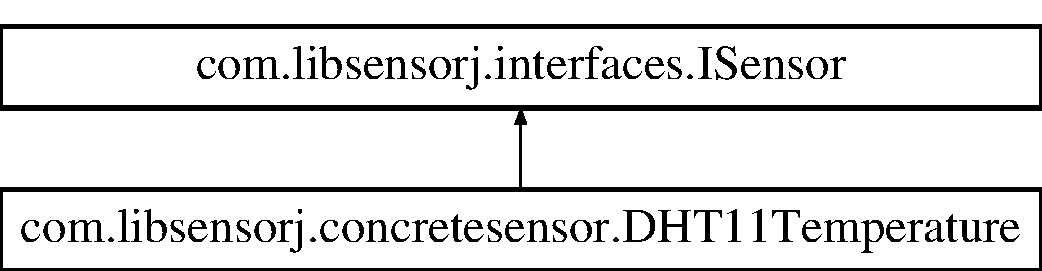
\includegraphics[height=2.000000cm]{classcom_1_1libsensorj_1_1concretesensor_1_1DHT11Temperature}
\end{center}
\end{figure}
\subsection*{Public Member Functions}
\begin{DoxyCompactItemize}
\item 
\hyperlink{classcom_1_1libsensorj_1_1concretesensor_1_1DHT11Temperature_a81324fa18ad12062d493a880f3fbda67}{D\+H\+T11\+Temperature} (int \hyperlink{classcom_1_1libsensorj_1_1concretesensor_1_1DHT11Temperature_a312572f2f0bad8b41d171481ef4e3138}{gpio\+Pin})
\item 
\hyperlink{classcom_1_1libsensorj_1_1concretesensor_1_1DHT11Temperature_a02bbdf30c922adcbde84597bf698ff41}{D\+H\+T11\+Temperature} ()
\item 
void \hyperlink{classcom_1_1libsensorj_1_1concretesensor_1_1DHT11Temperature_a599358623598fb0076dc0a2e07978f0b}{get\+Instance} ()
\item 
synchronized double \hyperlink{classcom_1_1libsensorj_1_1concretesensor_1_1DHT11Temperature_ab0b6a73583d9244271174a3d896f5ed3}{get\+Temperature\+In\+Celsius} ()
\item 
synchronized double \hyperlink{classcom_1_1libsensorj_1_1concretesensor_1_1DHT11Temperature_aa564f9c66609426711cbd0fbfe6837e3}{get\+Temperature\+In\+Fahrenheit} ()
\item 
synchronized double \hyperlink{classcom_1_1libsensorj_1_1concretesensor_1_1DHT11Temperature_a2c1a2bfaaf97612a862079979394ff34}{get\+Temperature\+In\+Kelvin} ()
\end{DoxyCompactItemize}
\subsection*{Private Member Functions}
\begin{DoxyCompactItemize}
\item 
void \hyperlink{classcom_1_1libsensorj_1_1concretesensor_1_1DHT11Temperature_a0ed494577e6a3c68dc737b60f926269d}{check\+For\+Updates} ()
\item 
double \hyperlink{classcom_1_1libsensorj_1_1concretesensor_1_1DHT11Temperature_abb836186013ae429e2cfde981154969b}{get\+Temperature} (Temperature\+Scale from)
\item 
double \hyperlink{classcom_1_1libsensorj_1_1concretesensor_1_1DHT11Temperature_a061220e6439c2014ab81384738c07734}{parse\+Temperature} (String value)
\item 
String \hyperlink{classcom_1_1libsensorj_1_1concretesensor_1_1DHT11Temperature_a2e5125c490d1b7b28a359cf702334fd7}{read\+Values} ()
\end{DoxyCompactItemize}
\subsection*{Private Attributes}
\begin{DoxyCompactItemize}
\item 
String \hyperlink{classcom_1_1libsensorj_1_1concretesensor_1_1DHT11Temperature_af16dd6a4c88dedacb8a4d69d90eff670}{last\+Value}
\item 
long \hyperlink{classcom_1_1libsensorj_1_1concretesensor_1_1DHT11Temperature_a00ec2e3e31bcaf04f497d5c503a84c5e}{last\+Check}
\item 
final int \hyperlink{classcom_1_1libsensorj_1_1concretesensor_1_1DHT11Temperature_a312572f2f0bad8b41d171481ef4e3138}{gpio\+Pin}
\end{DoxyCompactItemize}
\subsection*{Static Private Attributes}
\begin{DoxyCompactItemize}
\item 
static final String \hyperlink{classcom_1_1libsensorj_1_1concretesensor_1_1DHT11Temperature_a123ae6845e0cc1d1ec859cf7cfb78004}{T\+E\+M\+P\+\_\+\+S\+T\+R} = \char`\"{}Temp =\char`\"{}
\item 
static final int \hyperlink{classcom_1_1libsensorj_1_1concretesensor_1_1DHT11Temperature_af8bf5091500d4dcb3b5a0663279359e2}{D\+E\+F\+A\+U\+L\+T\+\_\+\+P\+I\+N} = 4
\item 
static final long \hyperlink{classcom_1_1libsensorj_1_1concretesensor_1_1DHT11Temperature_a7a5b6b6685407c05809a7e4c97358dd4}{L\+A\+S\+T\+\_\+\+C\+H\+E\+C\+K\+\_\+\+D\+I\+F\+F} = 3000
\item 
static final Logger \hyperlink{classcom_1_1libsensorj_1_1concretesensor_1_1DHT11Temperature_a96d485fc09496c1b5a320a30bb3400c9}{L\+O\+G\+G\+E\+R}
\end{DoxyCompactItemize}


\subsection{Detailed Description}
The Class \hyperlink{classcom_1_1libsensorj_1_1concretesensor_1_1DHT11Temperature}{D\+H\+T11\+Temperature}. 

\subsection{Constructor \& Destructor Documentation}
\hypertarget{classcom_1_1libsensorj_1_1concretesensor_1_1DHT11Temperature_a81324fa18ad12062d493a880f3fbda67}{}\index{com\+::libsensorj\+::concretesensor\+::\+D\+H\+T11\+Temperature@{com\+::libsensorj\+::concretesensor\+::\+D\+H\+T11\+Temperature}!D\+H\+T11\+Temperature@{D\+H\+T11\+Temperature}}
\index{D\+H\+T11\+Temperature@{D\+H\+T11\+Temperature}!com\+::libsensorj\+::concretesensor\+::\+D\+H\+T11\+Temperature@{com\+::libsensorj\+::concretesensor\+::\+D\+H\+T11\+Temperature}}
\subsubsection[{D\+H\+T11\+Temperature}]{\setlength{\rightskip}{0pt plus 5cm}com.\+libsensorj.\+concretesensor.\+D\+H\+T11\+Temperature.\+D\+H\+T11\+Temperature (
\begin{DoxyParamCaption}
\item[{int}]{gpio\+Pin}
\end{DoxyParamCaption}
)}\label{classcom_1_1libsensorj_1_1concretesensor_1_1DHT11Temperature_a81324fa18ad12062d493a880f3fbda67}
Instantiates a new D\+Ht11 temperature.


\begin{DoxyParams}{Parameters}
{\em gpio\+Pin} & the gpio pin \\
\hline
\end{DoxyParams}
\hypertarget{classcom_1_1libsensorj_1_1concretesensor_1_1DHT11Temperature_a02bbdf30c922adcbde84597bf698ff41}{}\index{com\+::libsensorj\+::concretesensor\+::\+D\+H\+T11\+Temperature@{com\+::libsensorj\+::concretesensor\+::\+D\+H\+T11\+Temperature}!D\+H\+T11\+Temperature@{D\+H\+T11\+Temperature}}
\index{D\+H\+T11\+Temperature@{D\+H\+T11\+Temperature}!com\+::libsensorj\+::concretesensor\+::\+D\+H\+T11\+Temperature@{com\+::libsensorj\+::concretesensor\+::\+D\+H\+T11\+Temperature}}
\subsubsection[{D\+H\+T11\+Temperature}]{\setlength{\rightskip}{0pt plus 5cm}com.\+libsensorj.\+concretesensor.\+D\+H\+T11\+Temperature.\+D\+H\+T11\+Temperature (
\begin{DoxyParamCaption}
{}
\end{DoxyParamCaption}
)}\label{classcom_1_1libsensorj_1_1concretesensor_1_1DHT11Temperature_a02bbdf30c922adcbde84597bf698ff41}
Instantiates a new D\+Ht11 temperature. 

\subsection{Member Function Documentation}
\hypertarget{classcom_1_1libsensorj_1_1concretesensor_1_1DHT11Temperature_a0ed494577e6a3c68dc737b60f926269d}{}\index{com\+::libsensorj\+::concretesensor\+::\+D\+H\+T11\+Temperature@{com\+::libsensorj\+::concretesensor\+::\+D\+H\+T11\+Temperature}!check\+For\+Updates@{check\+For\+Updates}}
\index{check\+For\+Updates@{check\+For\+Updates}!com\+::libsensorj\+::concretesensor\+::\+D\+H\+T11\+Temperature@{com\+::libsensorj\+::concretesensor\+::\+D\+H\+T11\+Temperature}}
\subsubsection[{check\+For\+Updates}]{\setlength{\rightskip}{0pt plus 5cm}void com.\+libsensorj.\+concretesensor.\+D\+H\+T11\+Temperature.\+check\+For\+Updates (
\begin{DoxyParamCaption}
{}
\end{DoxyParamCaption}
)\hspace{0.3cm}{\ttfamily [private]}}\label{classcom_1_1libsensorj_1_1concretesensor_1_1DHT11Temperature_a0ed494577e6a3c68dc737b60f926269d}
Check for updates. \hypertarget{classcom_1_1libsensorj_1_1concretesensor_1_1DHT11Temperature_a599358623598fb0076dc0a2e07978f0b}{}\index{com\+::libsensorj\+::concretesensor\+::\+D\+H\+T11\+Temperature@{com\+::libsensorj\+::concretesensor\+::\+D\+H\+T11\+Temperature}!get\+Instance@{get\+Instance}}
\index{get\+Instance@{get\+Instance}!com\+::libsensorj\+::concretesensor\+::\+D\+H\+T11\+Temperature@{com\+::libsensorj\+::concretesensor\+::\+D\+H\+T11\+Temperature}}
\subsubsection[{get\+Instance}]{\setlength{\rightskip}{0pt plus 5cm}void com.\+libsensorj.\+concretesensor.\+D\+H\+T11\+Temperature.\+get\+Instance (
\begin{DoxyParamCaption}
{}
\end{DoxyParamCaption}
)}\label{classcom_1_1libsensorj_1_1concretesensor_1_1DHT11Temperature_a599358623598fb0076dc0a2e07978f0b}
Gets the single instance of I\+Sensor.

\begin{DoxyReturn}{Returns}
single instance of I\+Sensor 
\end{DoxyReturn}


Implements \hyperlink{interfacecom_1_1libsensorj_1_1interfaces_1_1ISensor_a3c3db93a33adecde81a528651790f75e}{com.\+libsensorj.\+interfaces.\+I\+Sensor}.

\hypertarget{classcom_1_1libsensorj_1_1concretesensor_1_1DHT11Temperature_abb836186013ae429e2cfde981154969b}{}\index{com\+::libsensorj\+::concretesensor\+::\+D\+H\+T11\+Temperature@{com\+::libsensorj\+::concretesensor\+::\+D\+H\+T11\+Temperature}!get\+Temperature@{get\+Temperature}}
\index{get\+Temperature@{get\+Temperature}!com\+::libsensorj\+::concretesensor\+::\+D\+H\+T11\+Temperature@{com\+::libsensorj\+::concretesensor\+::\+D\+H\+T11\+Temperature}}
\subsubsection[{get\+Temperature}]{\setlength{\rightskip}{0pt plus 5cm}double com.\+libsensorj.\+concretesensor.\+D\+H\+T11\+Temperature.\+get\+Temperature (
\begin{DoxyParamCaption}
\item[{Temperature\+Scale}]{from}
\end{DoxyParamCaption}
)\hspace{0.3cm}{\ttfamily [private]}}\label{classcom_1_1libsensorj_1_1concretesensor_1_1DHT11Temperature_abb836186013ae429e2cfde981154969b}
Gets the temperature.


\begin{DoxyParams}{Parameters}
{\em from} & the from \\
\hline
\end{DoxyParams}
\begin{DoxyReturn}{Returns}
the temperature 
\end{DoxyReturn}
\hypertarget{classcom_1_1libsensorj_1_1concretesensor_1_1DHT11Temperature_ab0b6a73583d9244271174a3d896f5ed3}{}\index{com\+::libsensorj\+::concretesensor\+::\+D\+H\+T11\+Temperature@{com\+::libsensorj\+::concretesensor\+::\+D\+H\+T11\+Temperature}!get\+Temperature\+In\+Celsius@{get\+Temperature\+In\+Celsius}}
\index{get\+Temperature\+In\+Celsius@{get\+Temperature\+In\+Celsius}!com\+::libsensorj\+::concretesensor\+::\+D\+H\+T11\+Temperature@{com\+::libsensorj\+::concretesensor\+::\+D\+H\+T11\+Temperature}}
\subsubsection[{get\+Temperature\+In\+Celsius}]{\setlength{\rightskip}{0pt plus 5cm}synchronized double com.\+libsensorj.\+concretesensor.\+D\+H\+T11\+Temperature.\+get\+Temperature\+In\+Celsius (
\begin{DoxyParamCaption}
{}
\end{DoxyParamCaption}
)}\label{classcom_1_1libsensorj_1_1concretesensor_1_1DHT11Temperature_ab0b6a73583d9244271174a3d896f5ed3}
Gets the temperature in celsius.

\begin{DoxyReturn}{Returns}
the temperature in celsius 
\end{DoxyReturn}
\hypertarget{classcom_1_1libsensorj_1_1concretesensor_1_1DHT11Temperature_aa564f9c66609426711cbd0fbfe6837e3}{}\index{com\+::libsensorj\+::concretesensor\+::\+D\+H\+T11\+Temperature@{com\+::libsensorj\+::concretesensor\+::\+D\+H\+T11\+Temperature}!get\+Temperature\+In\+Fahrenheit@{get\+Temperature\+In\+Fahrenheit}}
\index{get\+Temperature\+In\+Fahrenheit@{get\+Temperature\+In\+Fahrenheit}!com\+::libsensorj\+::concretesensor\+::\+D\+H\+T11\+Temperature@{com\+::libsensorj\+::concretesensor\+::\+D\+H\+T11\+Temperature}}
\subsubsection[{get\+Temperature\+In\+Fahrenheit}]{\setlength{\rightskip}{0pt plus 5cm}synchronized double com.\+libsensorj.\+concretesensor.\+D\+H\+T11\+Temperature.\+get\+Temperature\+In\+Fahrenheit (
\begin{DoxyParamCaption}
{}
\end{DoxyParamCaption}
)}\label{classcom_1_1libsensorj_1_1concretesensor_1_1DHT11Temperature_aa564f9c66609426711cbd0fbfe6837e3}
Gets the temperature in fahrenheit.

\begin{DoxyReturn}{Returns}
the temperature in fahrenheit 
\end{DoxyReturn}
\hypertarget{classcom_1_1libsensorj_1_1concretesensor_1_1DHT11Temperature_a2c1a2bfaaf97612a862079979394ff34}{}\index{com\+::libsensorj\+::concretesensor\+::\+D\+H\+T11\+Temperature@{com\+::libsensorj\+::concretesensor\+::\+D\+H\+T11\+Temperature}!get\+Temperature\+In\+Kelvin@{get\+Temperature\+In\+Kelvin}}
\index{get\+Temperature\+In\+Kelvin@{get\+Temperature\+In\+Kelvin}!com\+::libsensorj\+::concretesensor\+::\+D\+H\+T11\+Temperature@{com\+::libsensorj\+::concretesensor\+::\+D\+H\+T11\+Temperature}}
\subsubsection[{get\+Temperature\+In\+Kelvin}]{\setlength{\rightskip}{0pt plus 5cm}synchronized double com.\+libsensorj.\+concretesensor.\+D\+H\+T11\+Temperature.\+get\+Temperature\+In\+Kelvin (
\begin{DoxyParamCaption}
{}
\end{DoxyParamCaption}
)}\label{classcom_1_1libsensorj_1_1concretesensor_1_1DHT11Temperature_a2c1a2bfaaf97612a862079979394ff34}
Gets the temperature in kelvin.

\begin{DoxyReturn}{Returns}
the temperature in kelvin 
\end{DoxyReturn}
\hypertarget{classcom_1_1libsensorj_1_1concretesensor_1_1DHT11Temperature_a061220e6439c2014ab81384738c07734}{}\index{com\+::libsensorj\+::concretesensor\+::\+D\+H\+T11\+Temperature@{com\+::libsensorj\+::concretesensor\+::\+D\+H\+T11\+Temperature}!parse\+Temperature@{parse\+Temperature}}
\index{parse\+Temperature@{parse\+Temperature}!com\+::libsensorj\+::concretesensor\+::\+D\+H\+T11\+Temperature@{com\+::libsensorj\+::concretesensor\+::\+D\+H\+T11\+Temperature}}
\subsubsection[{parse\+Temperature}]{\setlength{\rightskip}{0pt plus 5cm}double com.\+libsensorj.\+concretesensor.\+D\+H\+T11\+Temperature.\+parse\+Temperature (
\begin{DoxyParamCaption}
\item[{String}]{value}
\end{DoxyParamCaption}
)\hspace{0.3cm}{\ttfamily [private]}}\label{classcom_1_1libsensorj_1_1concretesensor_1_1DHT11Temperature_a061220e6439c2014ab81384738c07734}
Parses the temperature.


\begin{DoxyParams}{Parameters}
{\em value} & the value \\
\hline
\end{DoxyParams}
\begin{DoxyReturn}{Returns}
the double 
\end{DoxyReturn}
\hypertarget{classcom_1_1libsensorj_1_1concretesensor_1_1DHT11Temperature_a2e5125c490d1b7b28a359cf702334fd7}{}\index{com\+::libsensorj\+::concretesensor\+::\+D\+H\+T11\+Temperature@{com\+::libsensorj\+::concretesensor\+::\+D\+H\+T11\+Temperature}!read\+Values@{read\+Values}}
\index{read\+Values@{read\+Values}!com\+::libsensorj\+::concretesensor\+::\+D\+H\+T11\+Temperature@{com\+::libsensorj\+::concretesensor\+::\+D\+H\+T11\+Temperature}}
\subsubsection[{read\+Values}]{\setlength{\rightskip}{0pt plus 5cm}String com.\+libsensorj.\+concretesensor.\+D\+H\+T11\+Temperature.\+read\+Values (
\begin{DoxyParamCaption}
{}
\end{DoxyParamCaption}
)\hspace{0.3cm}{\ttfamily [private]}}\label{classcom_1_1libsensorj_1_1concretesensor_1_1DHT11Temperature_a2e5125c490d1b7b28a359cf702334fd7}
Read values.

\begin{DoxyReturn}{Returns}
the value readed as a string 
\end{DoxyReturn}


\subsection{Member Data Documentation}
\hypertarget{classcom_1_1libsensorj_1_1concretesensor_1_1DHT11Temperature_af8bf5091500d4dcb3b5a0663279359e2}{}\index{com\+::libsensorj\+::concretesensor\+::\+D\+H\+T11\+Temperature@{com\+::libsensorj\+::concretesensor\+::\+D\+H\+T11\+Temperature}!D\+E\+F\+A\+U\+L\+T\+\_\+\+P\+I\+N@{D\+E\+F\+A\+U\+L\+T\+\_\+\+P\+I\+N}}
\index{D\+E\+F\+A\+U\+L\+T\+\_\+\+P\+I\+N@{D\+E\+F\+A\+U\+L\+T\+\_\+\+P\+I\+N}!com\+::libsensorj\+::concretesensor\+::\+D\+H\+T11\+Temperature@{com\+::libsensorj\+::concretesensor\+::\+D\+H\+T11\+Temperature}}
\subsubsection[{D\+E\+F\+A\+U\+L\+T\+\_\+\+P\+I\+N}]{\setlength{\rightskip}{0pt plus 5cm}final int com.\+libsensorj.\+concretesensor.\+D\+H\+T11\+Temperature.\+D\+E\+F\+A\+U\+L\+T\+\_\+\+P\+I\+N = 4\hspace{0.3cm}{\ttfamily [static]}, {\ttfamily [private]}}\label{classcom_1_1libsensorj_1_1concretesensor_1_1DHT11Temperature_af8bf5091500d4dcb3b5a0663279359e2}
The Constant D\+E\+F\+A\+U\+L\+T\+\_\+\+P\+I\+N. \hypertarget{classcom_1_1libsensorj_1_1concretesensor_1_1DHT11Temperature_a312572f2f0bad8b41d171481ef4e3138}{}\index{com\+::libsensorj\+::concretesensor\+::\+D\+H\+T11\+Temperature@{com\+::libsensorj\+::concretesensor\+::\+D\+H\+T11\+Temperature}!gpio\+Pin@{gpio\+Pin}}
\index{gpio\+Pin@{gpio\+Pin}!com\+::libsensorj\+::concretesensor\+::\+D\+H\+T11\+Temperature@{com\+::libsensorj\+::concretesensor\+::\+D\+H\+T11\+Temperature}}
\subsubsection[{gpio\+Pin}]{\setlength{\rightskip}{0pt plus 5cm}final int com.\+libsensorj.\+concretesensor.\+D\+H\+T11\+Temperature.\+gpio\+Pin\hspace{0.3cm}{\ttfamily [private]}}\label{classcom_1_1libsensorj_1_1concretesensor_1_1DHT11Temperature_a312572f2f0bad8b41d171481ef4e3138}
The gpio pin. \hypertarget{classcom_1_1libsensorj_1_1concretesensor_1_1DHT11Temperature_a7a5b6b6685407c05809a7e4c97358dd4}{}\index{com\+::libsensorj\+::concretesensor\+::\+D\+H\+T11\+Temperature@{com\+::libsensorj\+::concretesensor\+::\+D\+H\+T11\+Temperature}!L\+A\+S\+T\+\_\+\+C\+H\+E\+C\+K\+\_\+\+D\+I\+F\+F@{L\+A\+S\+T\+\_\+\+C\+H\+E\+C\+K\+\_\+\+D\+I\+F\+F}}
\index{L\+A\+S\+T\+\_\+\+C\+H\+E\+C\+K\+\_\+\+D\+I\+F\+F@{L\+A\+S\+T\+\_\+\+C\+H\+E\+C\+K\+\_\+\+D\+I\+F\+F}!com\+::libsensorj\+::concretesensor\+::\+D\+H\+T11\+Temperature@{com\+::libsensorj\+::concretesensor\+::\+D\+H\+T11\+Temperature}}
\subsubsection[{L\+A\+S\+T\+\_\+\+C\+H\+E\+C\+K\+\_\+\+D\+I\+F\+F}]{\setlength{\rightskip}{0pt plus 5cm}final long com.\+libsensorj.\+concretesensor.\+D\+H\+T11\+Temperature.\+L\+A\+S\+T\+\_\+\+C\+H\+E\+C\+K\+\_\+\+D\+I\+F\+F = 3000\hspace{0.3cm}{\ttfamily [static]}, {\ttfamily [private]}}\label{classcom_1_1libsensorj_1_1concretesensor_1_1DHT11Temperature_a7a5b6b6685407c05809a7e4c97358dd4}
The Constant L\+A\+S\+T\+\_\+\+C\+H\+E\+C\+K\+\_\+\+D\+I\+F\+F. \hypertarget{classcom_1_1libsensorj_1_1concretesensor_1_1DHT11Temperature_a00ec2e3e31bcaf04f497d5c503a84c5e}{}\index{com\+::libsensorj\+::concretesensor\+::\+D\+H\+T11\+Temperature@{com\+::libsensorj\+::concretesensor\+::\+D\+H\+T11\+Temperature}!last\+Check@{last\+Check}}
\index{last\+Check@{last\+Check}!com\+::libsensorj\+::concretesensor\+::\+D\+H\+T11\+Temperature@{com\+::libsensorj\+::concretesensor\+::\+D\+H\+T11\+Temperature}}
\subsubsection[{last\+Check}]{\setlength{\rightskip}{0pt plus 5cm}long com.\+libsensorj.\+concretesensor.\+D\+H\+T11\+Temperature.\+last\+Check\hspace{0.3cm}{\ttfamily [private]}}\label{classcom_1_1libsensorj_1_1concretesensor_1_1DHT11Temperature_a00ec2e3e31bcaf04f497d5c503a84c5e}
The last check. \hypertarget{classcom_1_1libsensorj_1_1concretesensor_1_1DHT11Temperature_af16dd6a4c88dedacb8a4d69d90eff670}{}\index{com\+::libsensorj\+::concretesensor\+::\+D\+H\+T11\+Temperature@{com\+::libsensorj\+::concretesensor\+::\+D\+H\+T11\+Temperature}!last\+Value@{last\+Value}}
\index{last\+Value@{last\+Value}!com\+::libsensorj\+::concretesensor\+::\+D\+H\+T11\+Temperature@{com\+::libsensorj\+::concretesensor\+::\+D\+H\+T11\+Temperature}}
\subsubsection[{last\+Value}]{\setlength{\rightskip}{0pt plus 5cm}String com.\+libsensorj.\+concretesensor.\+D\+H\+T11\+Temperature.\+last\+Value\hspace{0.3cm}{\ttfamily [private]}}\label{classcom_1_1libsensorj_1_1concretesensor_1_1DHT11Temperature_af16dd6a4c88dedacb8a4d69d90eff670}
The last value. \hypertarget{classcom_1_1libsensorj_1_1concretesensor_1_1DHT11Temperature_a96d485fc09496c1b5a320a30bb3400c9}{}\index{com\+::libsensorj\+::concretesensor\+::\+D\+H\+T11\+Temperature@{com\+::libsensorj\+::concretesensor\+::\+D\+H\+T11\+Temperature}!L\+O\+G\+G\+E\+R@{L\+O\+G\+G\+E\+R}}
\index{L\+O\+G\+G\+E\+R@{L\+O\+G\+G\+E\+R}!com\+::libsensorj\+::concretesensor\+::\+D\+H\+T11\+Temperature@{com\+::libsensorj\+::concretesensor\+::\+D\+H\+T11\+Temperature}}
\subsubsection[{L\+O\+G\+G\+E\+R}]{\setlength{\rightskip}{0pt plus 5cm}final Logger com.\+libsensorj.\+concretesensor.\+D\+H\+T11\+Temperature.\+L\+O\+G\+G\+E\+R\hspace{0.3cm}{\ttfamily [static]}, {\ttfamily [private]}}\label{classcom_1_1libsensorj_1_1concretesensor_1_1DHT11Temperature_a96d485fc09496c1b5a320a30bb3400c9}
{\bfseries Initial value\+:}
\begin{DoxyCode}
= LogManager
            .getLogger(\hyperlink{classcom_1_1libsensorj_1_1concretesensor_1_1DHT11Temperature_a02bbdf30c922adcbde84597bf698ff41}{DHT11Temperature}.class.getName())
\end{DoxyCode}
The Constant L\+O\+G\+G\+E\+R. \hypertarget{classcom_1_1libsensorj_1_1concretesensor_1_1DHT11Temperature_a123ae6845e0cc1d1ec859cf7cfb78004}{}\index{com\+::libsensorj\+::concretesensor\+::\+D\+H\+T11\+Temperature@{com\+::libsensorj\+::concretesensor\+::\+D\+H\+T11\+Temperature}!T\+E\+M\+P\+\_\+\+S\+T\+R@{T\+E\+M\+P\+\_\+\+S\+T\+R}}
\index{T\+E\+M\+P\+\_\+\+S\+T\+R@{T\+E\+M\+P\+\_\+\+S\+T\+R}!com\+::libsensorj\+::concretesensor\+::\+D\+H\+T11\+Temperature@{com\+::libsensorj\+::concretesensor\+::\+D\+H\+T11\+Temperature}}
\subsubsection[{T\+E\+M\+P\+\_\+\+S\+T\+R}]{\setlength{\rightskip}{0pt plus 5cm}final String com.\+libsensorj.\+concretesensor.\+D\+H\+T11\+Temperature.\+T\+E\+M\+P\+\_\+\+S\+T\+R = \char`\"{}Temp =\char`\"{}\hspace{0.3cm}{\ttfamily [static]}, {\ttfamily [private]}}\label{classcom_1_1libsensorj_1_1concretesensor_1_1DHT11Temperature_a123ae6845e0cc1d1ec859cf7cfb78004}
The Constant T\+E\+M\+P\+\_\+\+S\+T\+R. 

The documentation for this class was generated from the following file\+:\begin{DoxyCompactItemize}
\item 
main/java/com/libsensorj/concretesensor/\hyperlink{DHT11Temperature_8java}{D\+H\+T11\+Temperature.\+java}\end{DoxyCompactItemize}

\hypertarget{classcom_1_1libsensorj_1_1examples_1_1DHT11TemperatureExample}{}\section{com.\+libsensorj.\+examples.\+D\+H\+T11\+Temperature\+Example Class Reference}
\label{classcom_1_1libsensorj_1_1examples_1_1DHT11TemperatureExample}\index{com.\+libsensorj.\+examples.\+D\+H\+T11\+Temperature\+Example@{com.\+libsensorj.\+examples.\+D\+H\+T11\+Temperature\+Example}}
\subsection*{Static Public Member Functions}
\begin{DoxyCompactItemize}
\item 
static void \hyperlink{classcom_1_1libsensorj_1_1examples_1_1DHT11TemperatureExample_a436567d5cd7d4e55dbed6438386af490}{main} (String\mbox{[}$\,$\mbox{]} args)
\end{DoxyCompactItemize}
\subsection*{Static Private Attributes}
\begin{DoxyCompactItemize}
\item 
static \hyperlink{interfacecom_1_1libsensorj_1_1interfaces_1_1ISensor}{I\+Sensor} \hyperlink{classcom_1_1libsensorj_1_1examples_1_1DHT11TemperatureExample_ae5b24da8a75b04b9f313d9b4aaa2f058}{dht11}
\end{DoxyCompactItemize}


\subsection{Member Function Documentation}
\hypertarget{classcom_1_1libsensorj_1_1examples_1_1DHT11TemperatureExample_a436567d5cd7d4e55dbed6438386af490}{}\index{com\+::libsensorj\+::examples\+::\+D\+H\+T11\+Temperature\+Example@{com\+::libsensorj\+::examples\+::\+D\+H\+T11\+Temperature\+Example}!main@{main}}
\index{main@{main}!com\+::libsensorj\+::examples\+::\+D\+H\+T11\+Temperature\+Example@{com\+::libsensorj\+::examples\+::\+D\+H\+T11\+Temperature\+Example}}
\subsubsection[{main}]{\setlength{\rightskip}{0pt plus 5cm}static void com.\+libsensorj.\+examples.\+D\+H\+T11\+Temperature\+Example.\+main (
\begin{DoxyParamCaption}
\item[{String\mbox{[}$\,$\mbox{]}}]{args}
\end{DoxyParamCaption}
)\hspace{0.3cm}{\ttfamily [static]}}\label{classcom_1_1libsensorj_1_1examples_1_1DHT11TemperatureExample_a436567d5cd7d4e55dbed6438386af490}


\subsection{Member Data Documentation}
\hypertarget{classcom_1_1libsensorj_1_1examples_1_1DHT11TemperatureExample_ae5b24da8a75b04b9f313d9b4aaa2f058}{}\index{com\+::libsensorj\+::examples\+::\+D\+H\+T11\+Temperature\+Example@{com\+::libsensorj\+::examples\+::\+D\+H\+T11\+Temperature\+Example}!dht11@{dht11}}
\index{dht11@{dht11}!com\+::libsensorj\+::examples\+::\+D\+H\+T11\+Temperature\+Example@{com\+::libsensorj\+::examples\+::\+D\+H\+T11\+Temperature\+Example}}
\subsubsection[{dht11}]{\setlength{\rightskip}{0pt plus 5cm}{\bf I\+Sensor} com.\+libsensorj.\+examples.\+D\+H\+T11\+Temperature\+Example.\+dht11\hspace{0.3cm}{\ttfamily [static]}, {\ttfamily [private]}}\label{classcom_1_1libsensorj_1_1examples_1_1DHT11TemperatureExample_ae5b24da8a75b04b9f313d9b4aaa2f058}


The documentation for this class was generated from the following file\+:\begin{DoxyCompactItemize}
\item 
main/java/com/libsensorj/examples/\hyperlink{DHT11TemperatureExample_8java}{D\+H\+T11\+Temperature\+Example.\+java}\end{DoxyCompactItemize}

\hypertarget{classcom_1_1libsensorj_1_1concretesensor_1_1test_1_1DHT11TemperatureTests}{}\section{com.\+libsensorj.\+concretesensor.\+test.\+D\+H\+T11\+Temperature\+Tests Class Reference}
\label{classcom_1_1libsensorj_1_1concretesensor_1_1test_1_1DHT11TemperatureTests}\index{com.\+libsensorj.\+concretesensor.\+test.\+D\+H\+T11\+Temperature\+Tests@{com.\+libsensorj.\+concretesensor.\+test.\+D\+H\+T11\+Temperature\+Tests}}
\subsection*{Public Member Functions}
\begin{DoxyCompactItemize}
\item 
void \hyperlink{classcom_1_1libsensorj_1_1concretesensor_1_1test_1_1DHT11TemperatureTests_a45f30914d4e9956bd21d0e2b5f05554d}{test\+Pin\+Provisioned} ()
\item 
void \hyperlink{classcom_1_1libsensorj_1_1concretesensor_1_1test_1_1DHT11TemperatureTests_a34d4111d60b72ecf413072fe5069ab4c}{test\+Get\+Temperature\+In\+Celsius} ()
\item 
void \hyperlink{classcom_1_1libsensorj_1_1concretesensor_1_1test_1_1DHT11TemperatureTests_a1e1ecc5c963b8cbf3e882e925fcf9bad}{test\+Get\+Temperature\+In\+Fahrenheit} ()
\item 
void \hyperlink{classcom_1_1libsensorj_1_1concretesensor_1_1test_1_1DHT11TemperatureTests_a47e9ab518974b27fa28b0fde184193ea}{test\+Get\+Temperature\+In\+Kelvin} ()
\end{DoxyCompactItemize}
\subsection*{Static Public Member Functions}
\begin{DoxyCompactItemize}
\item 
static void \hyperlink{classcom_1_1libsensorj_1_1concretesensor_1_1test_1_1DHT11TemperatureTests_a1bc150d93e863d5d10ec0a16ae44779b}{setup} ()
\end{DoxyCompactItemize}
\subsection*{Static Private Attributes}
\begin{DoxyCompactItemize}
\item 
static Gpio\+Controller \hyperlink{classcom_1_1libsensorj_1_1concretesensor_1_1test_1_1DHT11TemperatureTests_a7de266694c33835d976bfcd36c973ab6}{gpio}
\item 
static Gpio\+Pin\+Digital\+Input \hyperlink{classcom_1_1libsensorj_1_1concretesensor_1_1test_1_1DHT11TemperatureTests_a539cfe245f8a95e61ba9fbee05ae4f22}{pin}
\item 
static Pin\+State \hyperlink{classcom_1_1libsensorj_1_1concretesensor_1_1test_1_1DHT11TemperatureTests_a0b1e8ff10deeef685ecc52fe4254e239}{pin\+Monitored\+State}
\item 
static final String \hyperlink{classcom_1_1libsensorj_1_1concretesensor_1_1test_1_1DHT11TemperatureTests_a59d2eecae4aa5084dfdc56ec6ddad4c4}{D\+A\+T\+A\+\_\+\+R\+E\+A\+D\+E\+D} = \char`\"{}Using \hyperlink{classcom_1_1libsensorj_1_1concretesensor_1_1test_1_1DHT11TemperatureTests_a539cfe245f8a95e61ba9fbee05ae4f22}{pin} \#4\+Data (40)\+: 0x32 0x0 0x1d 0x0 0x4f\+Temp = 29 $\ast$\+C, Hum = 50 \%\char`\"{}
\item 
static final String \hyperlink{classcom_1_1libsensorj_1_1concretesensor_1_1test_1_1DHT11TemperatureTests_a2e6886cd64d8982ff792d10404bca66f}{R\+E\+A\+D\+V\+A\+L\+U\+E\+S\+\_\+\+M\+E\+T\+H\+O\+D} = \char`\"{}read\+Values\char`\"{}
\item 
static final Logger \hyperlink{classcom_1_1libsensorj_1_1concretesensor_1_1test_1_1DHT11TemperatureTests_a12743e84b5d8a4c300c1ef20c6f7eed4}{L\+O\+G\+G\+E\+R}
\end{DoxyCompactItemize}


\subsection{Detailed Description}
The Class \hyperlink{classcom_1_1libsensorj_1_1concretesensor_1_1test_1_1DHT11TemperatureTests}{D\+H\+T11\+Temperature\+Tests}. 

\subsection{Member Function Documentation}
\hypertarget{classcom_1_1libsensorj_1_1concretesensor_1_1test_1_1DHT11TemperatureTests_a1bc150d93e863d5d10ec0a16ae44779b}{}\index{com\+::libsensorj\+::concretesensor\+::test\+::\+D\+H\+T11\+Temperature\+Tests@{com\+::libsensorj\+::concretesensor\+::test\+::\+D\+H\+T11\+Temperature\+Tests}!setup@{setup}}
\index{setup@{setup}!com\+::libsensorj\+::concretesensor\+::test\+::\+D\+H\+T11\+Temperature\+Tests@{com\+::libsensorj\+::concretesensor\+::test\+::\+D\+H\+T11\+Temperature\+Tests}}
\subsubsection[{setup}]{\setlength{\rightskip}{0pt plus 5cm}static void com.\+libsensorj.\+concretesensor.\+test.\+D\+H\+T11\+Temperature\+Tests.\+setup (
\begin{DoxyParamCaption}
{}
\end{DoxyParamCaption}
)\hspace{0.3cm}{\ttfamily [static]}}\label{classcom_1_1libsensorj_1_1concretesensor_1_1test_1_1DHT11TemperatureTests_a1bc150d93e863d5d10ec0a16ae44779b}
Setup. \hypertarget{classcom_1_1libsensorj_1_1concretesensor_1_1test_1_1DHT11TemperatureTests_a34d4111d60b72ecf413072fe5069ab4c}{}\index{com\+::libsensorj\+::concretesensor\+::test\+::\+D\+H\+T11\+Temperature\+Tests@{com\+::libsensorj\+::concretesensor\+::test\+::\+D\+H\+T11\+Temperature\+Tests}!test\+Get\+Temperature\+In\+Celsius@{test\+Get\+Temperature\+In\+Celsius}}
\index{test\+Get\+Temperature\+In\+Celsius@{test\+Get\+Temperature\+In\+Celsius}!com\+::libsensorj\+::concretesensor\+::test\+::\+D\+H\+T11\+Temperature\+Tests@{com\+::libsensorj\+::concretesensor\+::test\+::\+D\+H\+T11\+Temperature\+Tests}}
\subsubsection[{test\+Get\+Temperature\+In\+Celsius}]{\setlength{\rightskip}{0pt plus 5cm}void com.\+libsensorj.\+concretesensor.\+test.\+D\+H\+T11\+Temperature\+Tests.\+test\+Get\+Temperature\+In\+Celsius (
\begin{DoxyParamCaption}
{}
\end{DoxyParamCaption}
)}\label{classcom_1_1libsensorj_1_1concretesensor_1_1test_1_1DHT11TemperatureTests_a34d4111d60b72ecf413072fe5069ab4c}
Test Get\+Temperature\+In\+Celsius. \hypertarget{classcom_1_1libsensorj_1_1concretesensor_1_1test_1_1DHT11TemperatureTests_a1e1ecc5c963b8cbf3e882e925fcf9bad}{}\index{com\+::libsensorj\+::concretesensor\+::test\+::\+D\+H\+T11\+Temperature\+Tests@{com\+::libsensorj\+::concretesensor\+::test\+::\+D\+H\+T11\+Temperature\+Tests}!test\+Get\+Temperature\+In\+Fahrenheit@{test\+Get\+Temperature\+In\+Fahrenheit}}
\index{test\+Get\+Temperature\+In\+Fahrenheit@{test\+Get\+Temperature\+In\+Fahrenheit}!com\+::libsensorj\+::concretesensor\+::test\+::\+D\+H\+T11\+Temperature\+Tests@{com\+::libsensorj\+::concretesensor\+::test\+::\+D\+H\+T11\+Temperature\+Tests}}
\subsubsection[{test\+Get\+Temperature\+In\+Fahrenheit}]{\setlength{\rightskip}{0pt plus 5cm}void com.\+libsensorj.\+concretesensor.\+test.\+D\+H\+T11\+Temperature\+Tests.\+test\+Get\+Temperature\+In\+Fahrenheit (
\begin{DoxyParamCaption}
{}
\end{DoxyParamCaption}
)}\label{classcom_1_1libsensorj_1_1concretesensor_1_1test_1_1DHT11TemperatureTests_a1e1ecc5c963b8cbf3e882e925fcf9bad}
Test Get\+Temperature\+In\+Fahrenheit. \hypertarget{classcom_1_1libsensorj_1_1concretesensor_1_1test_1_1DHT11TemperatureTests_a47e9ab518974b27fa28b0fde184193ea}{}\index{com\+::libsensorj\+::concretesensor\+::test\+::\+D\+H\+T11\+Temperature\+Tests@{com\+::libsensorj\+::concretesensor\+::test\+::\+D\+H\+T11\+Temperature\+Tests}!test\+Get\+Temperature\+In\+Kelvin@{test\+Get\+Temperature\+In\+Kelvin}}
\index{test\+Get\+Temperature\+In\+Kelvin@{test\+Get\+Temperature\+In\+Kelvin}!com\+::libsensorj\+::concretesensor\+::test\+::\+D\+H\+T11\+Temperature\+Tests@{com\+::libsensorj\+::concretesensor\+::test\+::\+D\+H\+T11\+Temperature\+Tests}}
\subsubsection[{test\+Get\+Temperature\+In\+Kelvin}]{\setlength{\rightskip}{0pt plus 5cm}void com.\+libsensorj.\+concretesensor.\+test.\+D\+H\+T11\+Temperature\+Tests.\+test\+Get\+Temperature\+In\+Kelvin (
\begin{DoxyParamCaption}
{}
\end{DoxyParamCaption}
)}\label{classcom_1_1libsensorj_1_1concretesensor_1_1test_1_1DHT11TemperatureTests_a47e9ab518974b27fa28b0fde184193ea}
Test Get\+Temperature\+In\+Kelvin. \hypertarget{classcom_1_1libsensorj_1_1concretesensor_1_1test_1_1DHT11TemperatureTests_a45f30914d4e9956bd21d0e2b5f05554d}{}\index{com\+::libsensorj\+::concretesensor\+::test\+::\+D\+H\+T11\+Temperature\+Tests@{com\+::libsensorj\+::concretesensor\+::test\+::\+D\+H\+T11\+Temperature\+Tests}!test\+Pin\+Provisioned@{test\+Pin\+Provisioned}}
\index{test\+Pin\+Provisioned@{test\+Pin\+Provisioned}!com\+::libsensorj\+::concretesensor\+::test\+::\+D\+H\+T11\+Temperature\+Tests@{com\+::libsensorj\+::concretesensor\+::test\+::\+D\+H\+T11\+Temperature\+Tests}}
\subsubsection[{test\+Pin\+Provisioned}]{\setlength{\rightskip}{0pt plus 5cm}void com.\+libsensorj.\+concretesensor.\+test.\+D\+H\+T11\+Temperature\+Tests.\+test\+Pin\+Provisioned (
\begin{DoxyParamCaption}
{}
\end{DoxyParamCaption}
)}\label{classcom_1_1libsensorj_1_1concretesensor_1_1test_1_1DHT11TemperatureTests_a45f30914d4e9956bd21d0e2b5f05554d}
Test pin provisioned. 

\subsection{Member Data Documentation}
\hypertarget{classcom_1_1libsensorj_1_1concretesensor_1_1test_1_1DHT11TemperatureTests_a59d2eecae4aa5084dfdc56ec6ddad4c4}{}\index{com\+::libsensorj\+::concretesensor\+::test\+::\+D\+H\+T11\+Temperature\+Tests@{com\+::libsensorj\+::concretesensor\+::test\+::\+D\+H\+T11\+Temperature\+Tests}!D\+A\+T\+A\+\_\+\+R\+E\+A\+D\+E\+D@{D\+A\+T\+A\+\_\+\+R\+E\+A\+D\+E\+D}}
\index{D\+A\+T\+A\+\_\+\+R\+E\+A\+D\+E\+D@{D\+A\+T\+A\+\_\+\+R\+E\+A\+D\+E\+D}!com\+::libsensorj\+::concretesensor\+::test\+::\+D\+H\+T11\+Temperature\+Tests@{com\+::libsensorj\+::concretesensor\+::test\+::\+D\+H\+T11\+Temperature\+Tests}}
\subsubsection[{D\+A\+T\+A\+\_\+\+R\+E\+A\+D\+E\+D}]{\setlength{\rightskip}{0pt plus 5cm}final String com.\+libsensorj.\+concretesensor.\+test.\+D\+H\+T11\+Temperature\+Tests.\+D\+A\+T\+A\+\_\+\+R\+E\+A\+D\+E\+D = \char`\"{}Using {\bf pin} \#4\+Data (40)\+: 0x32 0x0 0x1d 0x0 0x4f\+Temp = 29 $\ast$\+C, Hum = 50 \%\char`\"{}\hspace{0.3cm}{\ttfamily [static]}, {\ttfamily [private]}}\label{classcom_1_1libsensorj_1_1concretesensor_1_1test_1_1DHT11TemperatureTests_a59d2eecae4aa5084dfdc56ec6ddad4c4}
The Constant D\+A\+T\+A\+\_\+\+R\+E\+A\+D\+E\+D. \hypertarget{classcom_1_1libsensorj_1_1concretesensor_1_1test_1_1DHT11TemperatureTests_a7de266694c33835d976bfcd36c973ab6}{}\index{com\+::libsensorj\+::concretesensor\+::test\+::\+D\+H\+T11\+Temperature\+Tests@{com\+::libsensorj\+::concretesensor\+::test\+::\+D\+H\+T11\+Temperature\+Tests}!gpio@{gpio}}
\index{gpio@{gpio}!com\+::libsensorj\+::concretesensor\+::test\+::\+D\+H\+T11\+Temperature\+Tests@{com\+::libsensorj\+::concretesensor\+::test\+::\+D\+H\+T11\+Temperature\+Tests}}
\subsubsection[{gpio}]{\setlength{\rightskip}{0pt plus 5cm}Gpio\+Controller com.\+libsensorj.\+concretesensor.\+test.\+D\+H\+T11\+Temperature\+Tests.\+gpio\hspace{0.3cm}{\ttfamily [static]}, {\ttfamily [private]}}\label{classcom_1_1libsensorj_1_1concretesensor_1_1test_1_1DHT11TemperatureTests_a7de266694c33835d976bfcd36c973ab6}
The provider. The gpio. \hypertarget{classcom_1_1libsensorj_1_1concretesensor_1_1test_1_1DHT11TemperatureTests_a12743e84b5d8a4c300c1ef20c6f7eed4}{}\index{com\+::libsensorj\+::concretesensor\+::test\+::\+D\+H\+T11\+Temperature\+Tests@{com\+::libsensorj\+::concretesensor\+::test\+::\+D\+H\+T11\+Temperature\+Tests}!L\+O\+G\+G\+E\+R@{L\+O\+G\+G\+E\+R}}
\index{L\+O\+G\+G\+E\+R@{L\+O\+G\+G\+E\+R}!com\+::libsensorj\+::concretesensor\+::test\+::\+D\+H\+T11\+Temperature\+Tests@{com\+::libsensorj\+::concretesensor\+::test\+::\+D\+H\+T11\+Temperature\+Tests}}
\subsubsection[{L\+O\+G\+G\+E\+R}]{\setlength{\rightskip}{0pt plus 5cm}final Logger com.\+libsensorj.\+concretesensor.\+test.\+D\+H\+T11\+Temperature\+Tests.\+L\+O\+G\+G\+E\+R\hspace{0.3cm}{\ttfamily [static]}, {\ttfamily [private]}}\label{classcom_1_1libsensorj_1_1concretesensor_1_1test_1_1DHT11TemperatureTests_a12743e84b5d8a4c300c1ef20c6f7eed4}
{\bfseries Initial value\+:}
\begin{DoxyCode}
= LogManager
            .getLogger(DHT11TemperatureTests.class.getName())
\end{DoxyCode}
The Constant L\+O\+G\+G\+E\+R. \hypertarget{classcom_1_1libsensorj_1_1concretesensor_1_1test_1_1DHT11TemperatureTests_a539cfe245f8a95e61ba9fbee05ae4f22}{}\index{com\+::libsensorj\+::concretesensor\+::test\+::\+D\+H\+T11\+Temperature\+Tests@{com\+::libsensorj\+::concretesensor\+::test\+::\+D\+H\+T11\+Temperature\+Tests}!pin@{pin}}
\index{pin@{pin}!com\+::libsensorj\+::concretesensor\+::test\+::\+D\+H\+T11\+Temperature\+Tests@{com\+::libsensorj\+::concretesensor\+::test\+::\+D\+H\+T11\+Temperature\+Tests}}
\subsubsection[{pin}]{\setlength{\rightskip}{0pt plus 5cm}Gpio\+Pin\+Digital\+Input com.\+libsensorj.\+concretesensor.\+test.\+D\+H\+T11\+Temperature\+Tests.\+pin\hspace{0.3cm}{\ttfamily [static]}, {\ttfamily [private]}}\label{classcom_1_1libsensorj_1_1concretesensor_1_1test_1_1DHT11TemperatureTests_a539cfe245f8a95e61ba9fbee05ae4f22}
The pin. \hypertarget{classcom_1_1libsensorj_1_1concretesensor_1_1test_1_1DHT11TemperatureTests_a0b1e8ff10deeef685ecc52fe4254e239}{}\index{com\+::libsensorj\+::concretesensor\+::test\+::\+D\+H\+T11\+Temperature\+Tests@{com\+::libsensorj\+::concretesensor\+::test\+::\+D\+H\+T11\+Temperature\+Tests}!pin\+Monitored\+State@{pin\+Monitored\+State}}
\index{pin\+Monitored\+State@{pin\+Monitored\+State}!com\+::libsensorj\+::concretesensor\+::test\+::\+D\+H\+T11\+Temperature\+Tests@{com\+::libsensorj\+::concretesensor\+::test\+::\+D\+H\+T11\+Temperature\+Tests}}
\subsubsection[{pin\+Monitored\+State}]{\setlength{\rightskip}{0pt plus 5cm}Pin\+State com.\+libsensorj.\+concretesensor.\+test.\+D\+H\+T11\+Temperature\+Tests.\+pin\+Monitored\+State\hspace{0.3cm}{\ttfamily [static]}, {\ttfamily [private]}}\label{classcom_1_1libsensorj_1_1concretesensor_1_1test_1_1DHT11TemperatureTests_a0b1e8ff10deeef685ecc52fe4254e239}
The pin monitored state. \hypertarget{classcom_1_1libsensorj_1_1concretesensor_1_1test_1_1DHT11TemperatureTests_a2e6886cd64d8982ff792d10404bca66f}{}\index{com\+::libsensorj\+::concretesensor\+::test\+::\+D\+H\+T11\+Temperature\+Tests@{com\+::libsensorj\+::concretesensor\+::test\+::\+D\+H\+T11\+Temperature\+Tests}!R\+E\+A\+D\+V\+A\+L\+U\+E\+S\+\_\+\+M\+E\+T\+H\+O\+D@{R\+E\+A\+D\+V\+A\+L\+U\+E\+S\+\_\+\+M\+E\+T\+H\+O\+D}}
\index{R\+E\+A\+D\+V\+A\+L\+U\+E\+S\+\_\+\+M\+E\+T\+H\+O\+D@{R\+E\+A\+D\+V\+A\+L\+U\+E\+S\+\_\+\+M\+E\+T\+H\+O\+D}!com\+::libsensorj\+::concretesensor\+::test\+::\+D\+H\+T11\+Temperature\+Tests@{com\+::libsensorj\+::concretesensor\+::test\+::\+D\+H\+T11\+Temperature\+Tests}}
\subsubsection[{R\+E\+A\+D\+V\+A\+L\+U\+E\+S\+\_\+\+M\+E\+T\+H\+O\+D}]{\setlength{\rightskip}{0pt plus 5cm}final String com.\+libsensorj.\+concretesensor.\+test.\+D\+H\+T11\+Temperature\+Tests.\+R\+E\+A\+D\+V\+A\+L\+U\+E\+S\+\_\+\+M\+E\+T\+H\+O\+D = \char`\"{}read\+Values\char`\"{}\hspace{0.3cm}{\ttfamily [static]}, {\ttfamily [private]}}\label{classcom_1_1libsensorj_1_1concretesensor_1_1test_1_1DHT11TemperatureTests_a2e6886cd64d8982ff792d10404bca66f}
The Constant R\+E\+A\+D\+V\+A\+L\+U\+E\+S\+\_\+\+M\+E\+T\+H\+O\+D. 

The documentation for this class was generated from the following file\+:\begin{DoxyCompactItemize}
\item 
test/java/com/libsensorj/concretesensor/test/\hyperlink{DHT11TemperatureTests_8java}{D\+H\+T11\+Temperature\+Tests.\+java}\end{DoxyCompactItemize}

\hypertarget{classcom_1_1libsensorj_1_1concretesensor_1_1DHT11V2}{}\section{com.\+libsensorj.\+concretesensor.\+D\+H\+T11\+V2 Class Reference}
\label{classcom_1_1libsensorj_1_1concretesensor_1_1DHT11V2}\index{com.\+libsensorj.\+concretesensor.\+D\+H\+T11\+V2@{com.\+libsensorj.\+concretesensor.\+D\+H\+T11\+V2}}
Inheritance diagram for com.\+libsensorj.\+concretesensor.\+D\+H\+T11\+V2\+:\begin{figure}[H]
\begin{center}
\leavevmode
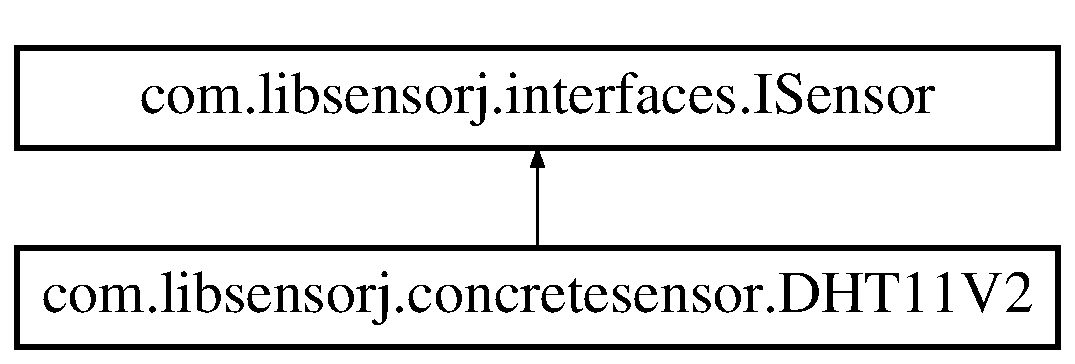
\includegraphics[height=2.000000cm]{classcom_1_1libsensorj_1_1concretesensor_1_1DHT11V2}
\end{center}
\end{figure}
\subsection*{Public Member Functions}
\begin{DoxyCompactItemize}
\item 
\hyperlink{classcom_1_1libsensorj_1_1concretesensor_1_1DHT11V2_a19e1a415c048669c7b4879e02d852682}{D\+H\+T11\+V2} ()
\item 
\hyperlink{classcom_1_1libsensorj_1_1concretesensor_1_1DHT11V2_a2c1a20a2c6796b8dd17629edaa9b4591}{D\+H\+T11\+V2} (int pin)
\item 
\hyperlink{classcom_1_1libsensorj_1_1concretesensor_1_1DHT11V2_a8c3dea8106eef93e12d61f7a7e32e5ca}{D\+H\+T11\+V2} (Pin pin)
\item 
double \hyperlink{classcom_1_1libsensorj_1_1concretesensor_1_1DHT11V2_a883913b8d65fc3e747e22374a8d16bc2}{read\+Value} ()
\item 
synchronized double \hyperlink{classcom_1_1libsensorj_1_1concretesensor_1_1DHT11V2_a3d5619f9ad57662d352dd9ddbf729a23}{get\+Temperature\+In\+Celsius} ()
\item 
synchronized double \hyperlink{classcom_1_1libsensorj_1_1concretesensor_1_1DHT11V2_aa1a825351fad9bd7b0c97abae4a89e05}{get\+Temperature\+In\+Fahrenheit} ()
\item 
synchronized double \hyperlink{classcom_1_1libsensorj_1_1concretesensor_1_1DHT11V2_a86989c9de8a041c8ca9f6f03c0714200}{get\+Temperature\+In\+Kelvin} ()
\item 
void \hyperlink{classcom_1_1libsensorj_1_1concretesensor_1_1DHT11V2_afff27f29285f26230faa8ecda6b6b102}{get\+Instance} ()
\end{DoxyCompactItemize}
\subsection*{Private Member Functions}
\begin{DoxyCompactItemize}
\item 
double \hyperlink{classcom_1_1libsensorj_1_1concretesensor_1_1DHT11V2_a4efa0044c366379af59e24b9570b3ddf}{get\+Temperature} (Temperature\+Scale from)
\item 
boolean \hyperlink{classcom_1_1libsensorj_1_1concretesensor_1_1DHT11V2_a250ebf2e29c3e9c84c840d6f6afc1c00}{check\+Parity} ()
\end{DoxyCompactItemize}
\subsection*{Private Attributes}
\begin{DoxyCompactItemize}
\item 
int\mbox{[}$\,$\mbox{]} \hyperlink{classcom_1_1libsensorj_1_1concretesensor_1_1DHT11V2_a450dd7dfb4fdc23cd25523ad22890ee4}{dht11\+Dat} = \{ 0, 0, 0, 0, 0 \}
\item 
Gpio\+Pin\+Digital\+Multipurpose \hyperlink{classcom_1_1libsensorj_1_1concretesensor_1_1DHT11V2_a04cca3ab141bcf0089fd6a7338a5dabe}{dht11\+Pin}
\end{DoxyCompactItemize}
\subsection*{Static Private Attributes}
\begin{DoxyCompactItemize}
\item 
static final Pin \hyperlink{classcom_1_1libsensorj_1_1concretesensor_1_1DHT11V2_a10e251a19e426166bb913323eee6243b}{D\+E\+F\+A\+U\+L\+T\+\_\+\+P\+I\+N} = Raspi\+Pin.\+G\+P\+I\+O\+\_\+04
\item 
static final int \hyperlink{classcom_1_1libsensorj_1_1concretesensor_1_1DHT11V2_ad64749b474c180fea185aecd512eb656}{M\+A\+X\+T\+I\+M\+I\+N\+G\+S} = 85
\item 
static final Logger \hyperlink{classcom_1_1libsensorj_1_1concretesensor_1_1DHT11V2_acef19b315279adf9b39a4407487d401e}{L\+O\+G\+G\+E\+R}
\end{DoxyCompactItemize}


\subsection{Detailed Description}
The Class \hyperlink{classcom_1_1libsensorj_1_1concretesensor_1_1DHT11V2}{D\+H\+T11\+V2}. 

\subsection{Constructor \& Destructor Documentation}
\hypertarget{classcom_1_1libsensorj_1_1concretesensor_1_1DHT11V2_a19e1a415c048669c7b4879e02d852682}{}\index{com\+::libsensorj\+::concretesensor\+::\+D\+H\+T11\+V2@{com\+::libsensorj\+::concretesensor\+::\+D\+H\+T11\+V2}!D\+H\+T11\+V2@{D\+H\+T11\+V2}}
\index{D\+H\+T11\+V2@{D\+H\+T11\+V2}!com\+::libsensorj\+::concretesensor\+::\+D\+H\+T11\+V2@{com\+::libsensorj\+::concretesensor\+::\+D\+H\+T11\+V2}}
\subsubsection[{D\+H\+T11\+V2}]{\setlength{\rightskip}{0pt plus 5cm}com.\+libsensorj.\+concretesensor.\+D\+H\+T11\+V2.\+D\+H\+T11\+V2 (
\begin{DoxyParamCaption}
{}
\end{DoxyParamCaption}
)}\label{classcom_1_1libsensorj_1_1concretesensor_1_1DHT11V2_a19e1a415c048669c7b4879e02d852682}
Instantiates a new D\+Ht11 v2. \hypertarget{classcom_1_1libsensorj_1_1concretesensor_1_1DHT11V2_a2c1a20a2c6796b8dd17629edaa9b4591}{}\index{com\+::libsensorj\+::concretesensor\+::\+D\+H\+T11\+V2@{com\+::libsensorj\+::concretesensor\+::\+D\+H\+T11\+V2}!D\+H\+T11\+V2@{D\+H\+T11\+V2}}
\index{D\+H\+T11\+V2@{D\+H\+T11\+V2}!com\+::libsensorj\+::concretesensor\+::\+D\+H\+T11\+V2@{com\+::libsensorj\+::concretesensor\+::\+D\+H\+T11\+V2}}
\subsubsection[{D\+H\+T11\+V2}]{\setlength{\rightskip}{0pt plus 5cm}com.\+libsensorj.\+concretesensor.\+D\+H\+T11\+V2.\+D\+H\+T11\+V2 (
\begin{DoxyParamCaption}
\item[{int}]{pin}
\end{DoxyParamCaption}
)}\label{classcom_1_1libsensorj_1_1concretesensor_1_1DHT11V2_a2c1a20a2c6796b8dd17629edaa9b4591}
Instantiates a new D\+Ht11 v2.


\begin{DoxyParams}{Parameters}
{\em pin} & the pin \\
\hline
\end{DoxyParams}
\hypertarget{classcom_1_1libsensorj_1_1concretesensor_1_1DHT11V2_a8c3dea8106eef93e12d61f7a7e32e5ca}{}\index{com\+::libsensorj\+::concretesensor\+::\+D\+H\+T11\+V2@{com\+::libsensorj\+::concretesensor\+::\+D\+H\+T11\+V2}!D\+H\+T11\+V2@{D\+H\+T11\+V2}}
\index{D\+H\+T11\+V2@{D\+H\+T11\+V2}!com\+::libsensorj\+::concretesensor\+::\+D\+H\+T11\+V2@{com\+::libsensorj\+::concretesensor\+::\+D\+H\+T11\+V2}}
\subsubsection[{D\+H\+T11\+V2}]{\setlength{\rightskip}{0pt plus 5cm}com.\+libsensorj.\+concretesensor.\+D\+H\+T11\+V2.\+D\+H\+T11\+V2 (
\begin{DoxyParamCaption}
\item[{Pin}]{pin}
\end{DoxyParamCaption}
)}\label{classcom_1_1libsensorj_1_1concretesensor_1_1DHT11V2_a8c3dea8106eef93e12d61f7a7e32e5ca}
Instantiates a new D\+Ht11 v2.


\begin{DoxyParams}{Parameters}
{\em pin} & the pin \\
\hline
\end{DoxyParams}


\subsection{Member Function Documentation}
\hypertarget{classcom_1_1libsensorj_1_1concretesensor_1_1DHT11V2_a250ebf2e29c3e9c84c840d6f6afc1c00}{}\index{com\+::libsensorj\+::concretesensor\+::\+D\+H\+T11\+V2@{com\+::libsensorj\+::concretesensor\+::\+D\+H\+T11\+V2}!check\+Parity@{check\+Parity}}
\index{check\+Parity@{check\+Parity}!com\+::libsensorj\+::concretesensor\+::\+D\+H\+T11\+V2@{com\+::libsensorj\+::concretesensor\+::\+D\+H\+T11\+V2}}
\subsubsection[{check\+Parity}]{\setlength{\rightskip}{0pt plus 5cm}boolean com.\+libsensorj.\+concretesensor.\+D\+H\+T11\+V2.\+check\+Parity (
\begin{DoxyParamCaption}
{}
\end{DoxyParamCaption}
)\hspace{0.3cm}{\ttfamily [private]}}\label{classcom_1_1libsensorj_1_1concretesensor_1_1DHT11V2_a250ebf2e29c3e9c84c840d6f6afc1c00}
Check parity.

\begin{DoxyReturn}{Returns}
true, if successful 
\end{DoxyReturn}
\hypertarget{classcom_1_1libsensorj_1_1concretesensor_1_1DHT11V2_afff27f29285f26230faa8ecda6b6b102}{}\index{com\+::libsensorj\+::concretesensor\+::\+D\+H\+T11\+V2@{com\+::libsensorj\+::concretesensor\+::\+D\+H\+T11\+V2}!get\+Instance@{get\+Instance}}
\index{get\+Instance@{get\+Instance}!com\+::libsensorj\+::concretesensor\+::\+D\+H\+T11\+V2@{com\+::libsensorj\+::concretesensor\+::\+D\+H\+T11\+V2}}
\subsubsection[{get\+Instance}]{\setlength{\rightskip}{0pt plus 5cm}void com.\+libsensorj.\+concretesensor.\+D\+H\+T11\+V2.\+get\+Instance (
\begin{DoxyParamCaption}
{}
\end{DoxyParamCaption}
)}\label{classcom_1_1libsensorj_1_1concretesensor_1_1DHT11V2_afff27f29285f26230faa8ecda6b6b102}
Gets the single instance of I\+Sensor.

\begin{DoxyReturn}{Returns}
single instance of I\+Sensor 
\end{DoxyReturn}


Implements \hyperlink{interfacecom_1_1libsensorj_1_1interfaces_1_1ISensor_a3c3db93a33adecde81a528651790f75e}{com.\+libsensorj.\+interfaces.\+I\+Sensor}.

\hypertarget{classcom_1_1libsensorj_1_1concretesensor_1_1DHT11V2_a4efa0044c366379af59e24b9570b3ddf}{}\index{com\+::libsensorj\+::concretesensor\+::\+D\+H\+T11\+V2@{com\+::libsensorj\+::concretesensor\+::\+D\+H\+T11\+V2}!get\+Temperature@{get\+Temperature}}
\index{get\+Temperature@{get\+Temperature}!com\+::libsensorj\+::concretesensor\+::\+D\+H\+T11\+V2@{com\+::libsensorj\+::concretesensor\+::\+D\+H\+T11\+V2}}
\subsubsection[{get\+Temperature}]{\setlength{\rightskip}{0pt plus 5cm}double com.\+libsensorj.\+concretesensor.\+D\+H\+T11\+V2.\+get\+Temperature (
\begin{DoxyParamCaption}
\item[{Temperature\+Scale}]{from}
\end{DoxyParamCaption}
)\hspace{0.3cm}{\ttfamily [private]}}\label{classcom_1_1libsensorj_1_1concretesensor_1_1DHT11V2_a4efa0044c366379af59e24b9570b3ddf}
Gets the temperature.


\begin{DoxyParams}{Parameters}
{\em from} & the from \\
\hline
\end{DoxyParams}
\begin{DoxyReturn}{Returns}
the temperature 
\end{DoxyReturn}
\hypertarget{classcom_1_1libsensorj_1_1concretesensor_1_1DHT11V2_a3d5619f9ad57662d352dd9ddbf729a23}{}\index{com\+::libsensorj\+::concretesensor\+::\+D\+H\+T11\+V2@{com\+::libsensorj\+::concretesensor\+::\+D\+H\+T11\+V2}!get\+Temperature\+In\+Celsius@{get\+Temperature\+In\+Celsius}}
\index{get\+Temperature\+In\+Celsius@{get\+Temperature\+In\+Celsius}!com\+::libsensorj\+::concretesensor\+::\+D\+H\+T11\+V2@{com\+::libsensorj\+::concretesensor\+::\+D\+H\+T11\+V2}}
\subsubsection[{get\+Temperature\+In\+Celsius}]{\setlength{\rightskip}{0pt plus 5cm}synchronized double com.\+libsensorj.\+concretesensor.\+D\+H\+T11\+V2.\+get\+Temperature\+In\+Celsius (
\begin{DoxyParamCaption}
{}
\end{DoxyParamCaption}
)}\label{classcom_1_1libsensorj_1_1concretesensor_1_1DHT11V2_a3d5619f9ad57662d352dd9ddbf729a23}
Gets the temperature in celsius.

\begin{DoxyReturn}{Returns}
the temperature in celsius 
\end{DoxyReturn}
\hypertarget{classcom_1_1libsensorj_1_1concretesensor_1_1DHT11V2_aa1a825351fad9bd7b0c97abae4a89e05}{}\index{com\+::libsensorj\+::concretesensor\+::\+D\+H\+T11\+V2@{com\+::libsensorj\+::concretesensor\+::\+D\+H\+T11\+V2}!get\+Temperature\+In\+Fahrenheit@{get\+Temperature\+In\+Fahrenheit}}
\index{get\+Temperature\+In\+Fahrenheit@{get\+Temperature\+In\+Fahrenheit}!com\+::libsensorj\+::concretesensor\+::\+D\+H\+T11\+V2@{com\+::libsensorj\+::concretesensor\+::\+D\+H\+T11\+V2}}
\subsubsection[{get\+Temperature\+In\+Fahrenheit}]{\setlength{\rightskip}{0pt plus 5cm}synchronized double com.\+libsensorj.\+concretesensor.\+D\+H\+T11\+V2.\+get\+Temperature\+In\+Fahrenheit (
\begin{DoxyParamCaption}
{}
\end{DoxyParamCaption}
)}\label{classcom_1_1libsensorj_1_1concretesensor_1_1DHT11V2_aa1a825351fad9bd7b0c97abae4a89e05}
Gets the temperature in fahrenheit.

\begin{DoxyReturn}{Returns}
the temperature in fahrenheit 
\end{DoxyReturn}
\hypertarget{classcom_1_1libsensorj_1_1concretesensor_1_1DHT11V2_a86989c9de8a041c8ca9f6f03c0714200}{}\index{com\+::libsensorj\+::concretesensor\+::\+D\+H\+T11\+V2@{com\+::libsensorj\+::concretesensor\+::\+D\+H\+T11\+V2}!get\+Temperature\+In\+Kelvin@{get\+Temperature\+In\+Kelvin}}
\index{get\+Temperature\+In\+Kelvin@{get\+Temperature\+In\+Kelvin}!com\+::libsensorj\+::concretesensor\+::\+D\+H\+T11\+V2@{com\+::libsensorj\+::concretesensor\+::\+D\+H\+T11\+V2}}
\subsubsection[{get\+Temperature\+In\+Kelvin}]{\setlength{\rightskip}{0pt plus 5cm}synchronized double com.\+libsensorj.\+concretesensor.\+D\+H\+T11\+V2.\+get\+Temperature\+In\+Kelvin (
\begin{DoxyParamCaption}
{}
\end{DoxyParamCaption}
)}\label{classcom_1_1libsensorj_1_1concretesensor_1_1DHT11V2_a86989c9de8a041c8ca9f6f03c0714200}
Gets the temperature in kelvin.

\begin{DoxyReturn}{Returns}
the temperature in kelvin 
\end{DoxyReturn}
\hypertarget{classcom_1_1libsensorj_1_1concretesensor_1_1DHT11V2_a883913b8d65fc3e747e22374a8d16bc2}{}\index{com\+::libsensorj\+::concretesensor\+::\+D\+H\+T11\+V2@{com\+::libsensorj\+::concretesensor\+::\+D\+H\+T11\+V2}!read\+Value@{read\+Value}}
\index{read\+Value@{read\+Value}!com\+::libsensorj\+::concretesensor\+::\+D\+H\+T11\+V2@{com\+::libsensorj\+::concretesensor\+::\+D\+H\+T11\+V2}}
\subsubsection[{read\+Value}]{\setlength{\rightskip}{0pt plus 5cm}double com.\+libsensorj.\+concretesensor.\+D\+H\+T11\+V2.\+read\+Value (
\begin{DoxyParamCaption}
{}
\end{DoxyParamCaption}
)}\label{classcom_1_1libsensorj_1_1concretesensor_1_1DHT11V2_a883913b8d65fc3e747e22374a8d16bc2}
Read value.

\begin{DoxyReturn}{Returns}
the value readed 
\end{DoxyReturn}


\subsection{Member Data Documentation}
\hypertarget{classcom_1_1libsensorj_1_1concretesensor_1_1DHT11V2_a10e251a19e426166bb913323eee6243b}{}\index{com\+::libsensorj\+::concretesensor\+::\+D\+H\+T11\+V2@{com\+::libsensorj\+::concretesensor\+::\+D\+H\+T11\+V2}!D\+E\+F\+A\+U\+L\+T\+\_\+\+P\+I\+N@{D\+E\+F\+A\+U\+L\+T\+\_\+\+P\+I\+N}}
\index{D\+E\+F\+A\+U\+L\+T\+\_\+\+P\+I\+N@{D\+E\+F\+A\+U\+L\+T\+\_\+\+P\+I\+N}!com\+::libsensorj\+::concretesensor\+::\+D\+H\+T11\+V2@{com\+::libsensorj\+::concretesensor\+::\+D\+H\+T11\+V2}}
\subsubsection[{D\+E\+F\+A\+U\+L\+T\+\_\+\+P\+I\+N}]{\setlength{\rightskip}{0pt plus 5cm}final Pin com.\+libsensorj.\+concretesensor.\+D\+H\+T11\+V2.\+D\+E\+F\+A\+U\+L\+T\+\_\+\+P\+I\+N = Raspi\+Pin.\+G\+P\+I\+O\+\_\+04\hspace{0.3cm}{\ttfamily [static]}, {\ttfamily [private]}}\label{classcom_1_1libsensorj_1_1concretesensor_1_1DHT11V2_a10e251a19e426166bb913323eee6243b}
The Constant D\+E\+F\+A\+U\+L\+T\+\_\+\+P\+I\+N. \hypertarget{classcom_1_1libsensorj_1_1concretesensor_1_1DHT11V2_a450dd7dfb4fdc23cd25523ad22890ee4}{}\index{com\+::libsensorj\+::concretesensor\+::\+D\+H\+T11\+V2@{com\+::libsensorj\+::concretesensor\+::\+D\+H\+T11\+V2}!dht11\+Dat@{dht11\+Dat}}
\index{dht11\+Dat@{dht11\+Dat}!com\+::libsensorj\+::concretesensor\+::\+D\+H\+T11\+V2@{com\+::libsensorj\+::concretesensor\+::\+D\+H\+T11\+V2}}
\subsubsection[{dht11\+Dat}]{\setlength{\rightskip}{0pt plus 5cm}int \mbox{[}$\,$\mbox{]} com.\+libsensorj.\+concretesensor.\+D\+H\+T11\+V2.\+dht11\+Dat = \{ 0, 0, 0, 0, 0 \}\hspace{0.3cm}{\ttfamily [private]}}\label{classcom_1_1libsensorj_1_1concretesensor_1_1DHT11V2_a450dd7dfb4fdc23cd25523ad22890ee4}
The dht11\+Dat. \hypertarget{classcom_1_1libsensorj_1_1concretesensor_1_1DHT11V2_a04cca3ab141bcf0089fd6a7338a5dabe}{}\index{com\+::libsensorj\+::concretesensor\+::\+D\+H\+T11\+V2@{com\+::libsensorj\+::concretesensor\+::\+D\+H\+T11\+V2}!dht11\+Pin@{dht11\+Pin}}
\index{dht11\+Pin@{dht11\+Pin}!com\+::libsensorj\+::concretesensor\+::\+D\+H\+T11\+V2@{com\+::libsensorj\+::concretesensor\+::\+D\+H\+T11\+V2}}
\subsubsection[{dht11\+Pin}]{\setlength{\rightskip}{0pt plus 5cm}Gpio\+Pin\+Digital\+Multipurpose com.\+libsensorj.\+concretesensor.\+D\+H\+T11\+V2.\+dht11\+Pin\hspace{0.3cm}{\ttfamily [private]}}\label{classcom_1_1libsensorj_1_1concretesensor_1_1DHT11V2_a04cca3ab141bcf0089fd6a7338a5dabe}
The dht11 pin. \hypertarget{classcom_1_1libsensorj_1_1concretesensor_1_1DHT11V2_acef19b315279adf9b39a4407487d401e}{}\index{com\+::libsensorj\+::concretesensor\+::\+D\+H\+T11\+V2@{com\+::libsensorj\+::concretesensor\+::\+D\+H\+T11\+V2}!L\+O\+G\+G\+E\+R@{L\+O\+G\+G\+E\+R}}
\index{L\+O\+G\+G\+E\+R@{L\+O\+G\+G\+E\+R}!com\+::libsensorj\+::concretesensor\+::\+D\+H\+T11\+V2@{com\+::libsensorj\+::concretesensor\+::\+D\+H\+T11\+V2}}
\subsubsection[{L\+O\+G\+G\+E\+R}]{\setlength{\rightskip}{0pt plus 5cm}final Logger com.\+libsensorj.\+concretesensor.\+D\+H\+T11\+V2.\+L\+O\+G\+G\+E\+R\hspace{0.3cm}{\ttfamily [static]}, {\ttfamily [private]}}\label{classcom_1_1libsensorj_1_1concretesensor_1_1DHT11V2_acef19b315279adf9b39a4407487d401e}
{\bfseries Initial value\+:}
\begin{DoxyCode}
= LogManager.getLogger(\hyperlink{classcom_1_1libsensorj_1_1concretesensor_1_1DHT11V2_a19e1a415c048669c7b4879e02d852682}{DHT11V2}.class
            .getName())
\end{DoxyCode}
The Constant L\+O\+G\+G\+E\+R. \hypertarget{classcom_1_1libsensorj_1_1concretesensor_1_1DHT11V2_ad64749b474c180fea185aecd512eb656}{}\index{com\+::libsensorj\+::concretesensor\+::\+D\+H\+T11\+V2@{com\+::libsensorj\+::concretesensor\+::\+D\+H\+T11\+V2}!M\+A\+X\+T\+I\+M\+I\+N\+G\+S@{M\+A\+X\+T\+I\+M\+I\+N\+G\+S}}
\index{M\+A\+X\+T\+I\+M\+I\+N\+G\+S@{M\+A\+X\+T\+I\+M\+I\+N\+G\+S}!com\+::libsensorj\+::concretesensor\+::\+D\+H\+T11\+V2@{com\+::libsensorj\+::concretesensor\+::\+D\+H\+T11\+V2}}
\subsubsection[{M\+A\+X\+T\+I\+M\+I\+N\+G\+S}]{\setlength{\rightskip}{0pt plus 5cm}final int com.\+libsensorj.\+concretesensor.\+D\+H\+T11\+V2.\+M\+A\+X\+T\+I\+M\+I\+N\+G\+S = 85\hspace{0.3cm}{\ttfamily [static]}, {\ttfamily [private]}}\label{classcom_1_1libsensorj_1_1concretesensor_1_1DHT11V2_ad64749b474c180fea185aecd512eb656}
The Constant M\+A\+X\+T\+I\+M\+I\+N\+G\+S. 

The documentation for this class was generated from the following file\+:\begin{DoxyCompactItemize}
\item 
main/java/com/libsensorj/concretesensor/\hyperlink{DHT11V2_8java}{D\+H\+T11\+V2.\+java}\end{DoxyCompactItemize}

\hypertarget{classcom_1_1libsensorj_1_1examples_1_1DHT11V2Example}{}\section{com.\+libsensorj.\+examples.\+D\+H\+T11\+V2\+Example Class Reference}
\label{classcom_1_1libsensorj_1_1examples_1_1DHT11V2Example}\index{com.\+libsensorj.\+examples.\+D\+H\+T11\+V2\+Example@{com.\+libsensorj.\+examples.\+D\+H\+T11\+V2\+Example}}
\subsection*{Static Public Member Functions}
\begin{DoxyCompactItemize}
\item 
static void \hyperlink{classcom_1_1libsensorj_1_1examples_1_1DHT11V2Example_a423db1184c15475e4b120b7f2783545b}{main} (String\mbox{[}$\,$\mbox{]} args)
\end{DoxyCompactItemize}
\subsection*{Static Private Attributes}
\begin{DoxyCompactItemize}
\item 
static \hyperlink{interfacecom_1_1libsensorj_1_1interfaces_1_1ISensor}{I\+Sensor} \hyperlink{classcom_1_1libsensorj_1_1examples_1_1DHT11V2Example_a5bc507916742167876ff258c298163ed}{dht11}
\item 
static final Logger \hyperlink{classcom_1_1libsensorj_1_1examples_1_1DHT11V2Example_a962cfebacb8855647655c3b6c0f6f698}{L\+O\+G\+G\+E\+R}
\end{DoxyCompactItemize}


\subsection{Detailed Description}
The Class \hyperlink{classcom_1_1libsensorj_1_1examples_1_1DHT11V2Example}{D\+H\+T11\+V2\+Example}. 

\subsection{Member Function Documentation}
\hypertarget{classcom_1_1libsensorj_1_1examples_1_1DHT11V2Example_a423db1184c15475e4b120b7f2783545b}{}\index{com\+::libsensorj\+::examples\+::\+D\+H\+T11\+V2\+Example@{com\+::libsensorj\+::examples\+::\+D\+H\+T11\+V2\+Example}!main@{main}}
\index{main@{main}!com\+::libsensorj\+::examples\+::\+D\+H\+T11\+V2\+Example@{com\+::libsensorj\+::examples\+::\+D\+H\+T11\+V2\+Example}}
\subsubsection[{main}]{\setlength{\rightskip}{0pt plus 5cm}static void com.\+libsensorj.\+examples.\+D\+H\+T11\+V2\+Example.\+main (
\begin{DoxyParamCaption}
\item[{String\mbox{[}$\,$\mbox{]}}]{args}
\end{DoxyParamCaption}
)\hspace{0.3cm}{\ttfamily [static]}}\label{classcom_1_1libsensorj_1_1examples_1_1DHT11V2Example_a423db1184c15475e4b120b7f2783545b}
The main method.


\begin{DoxyParams}{Parameters}
{\em args} & the arguments \\
\hline
\end{DoxyParams}


\subsection{Member Data Documentation}
\hypertarget{classcom_1_1libsensorj_1_1examples_1_1DHT11V2Example_a5bc507916742167876ff258c298163ed}{}\index{com\+::libsensorj\+::examples\+::\+D\+H\+T11\+V2\+Example@{com\+::libsensorj\+::examples\+::\+D\+H\+T11\+V2\+Example}!dht11@{dht11}}
\index{dht11@{dht11}!com\+::libsensorj\+::examples\+::\+D\+H\+T11\+V2\+Example@{com\+::libsensorj\+::examples\+::\+D\+H\+T11\+V2\+Example}}
\subsubsection[{dht11}]{\setlength{\rightskip}{0pt plus 5cm}{\bf I\+Sensor} com.\+libsensorj.\+examples.\+D\+H\+T11\+V2\+Example.\+dht11\hspace{0.3cm}{\ttfamily [static]}, {\ttfamily [private]}}\label{classcom_1_1libsensorj_1_1examples_1_1DHT11V2Example_a5bc507916742167876ff258c298163ed}
The I\+Sensor dht11. \hypertarget{classcom_1_1libsensorj_1_1examples_1_1DHT11V2Example_a962cfebacb8855647655c3b6c0f6f698}{}\index{com\+::libsensorj\+::examples\+::\+D\+H\+T11\+V2\+Example@{com\+::libsensorj\+::examples\+::\+D\+H\+T11\+V2\+Example}!L\+O\+G\+G\+E\+R@{L\+O\+G\+G\+E\+R}}
\index{L\+O\+G\+G\+E\+R@{L\+O\+G\+G\+E\+R}!com\+::libsensorj\+::examples\+::\+D\+H\+T11\+V2\+Example@{com\+::libsensorj\+::examples\+::\+D\+H\+T11\+V2\+Example}}
\subsubsection[{L\+O\+G\+G\+E\+R}]{\setlength{\rightskip}{0pt plus 5cm}final Logger com.\+libsensorj.\+examples.\+D\+H\+T11\+V2\+Example.\+L\+O\+G\+G\+E\+R\hspace{0.3cm}{\ttfamily [static]}, {\ttfamily [private]}}\label{classcom_1_1libsensorj_1_1examples_1_1DHT11V2Example_a962cfebacb8855647655c3b6c0f6f698}
{\bfseries Initial value\+:}
\begin{DoxyCode}
= LogManager
            .getLogger(DHT11TemperatureExample.class.getName())
\end{DoxyCode}
The Constant L\+O\+G\+G\+E\+R. 

The documentation for this class was generated from the following file\+:\begin{DoxyCompactItemize}
\item 
main/java/com/libsensorj/examples/\hyperlink{DHT11V2Example_8java}{D\+H\+T11\+V2\+Example.\+java}\end{DoxyCompactItemize}

\hypertarget{classcom_1_1libsensorj_1_1concretefactory_1_1DHT11V2Factory}{}\section{com.\+libsensorj.\+concretefactory.\+D\+H\+T11\+V2\+Factory Class Reference}
\label{classcom_1_1libsensorj_1_1concretefactory_1_1DHT11V2Factory}\index{com.\+libsensorj.\+concretefactory.\+D\+H\+T11\+V2\+Factory@{com.\+libsensorj.\+concretefactory.\+D\+H\+T11\+V2\+Factory}}
Inheritance diagram for com.\+libsensorj.\+concretefactory.\+D\+H\+T11\+V2\+Factory\+:\begin{figure}[H]
\begin{center}
\leavevmode
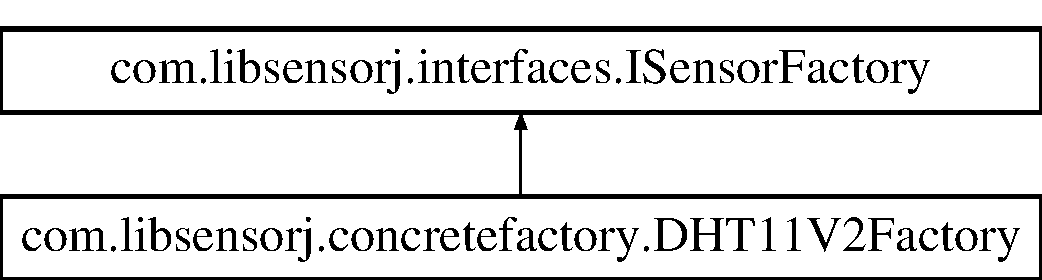
\includegraphics[height=2.000000cm]{classcom_1_1libsensorj_1_1concretefactory_1_1DHT11V2Factory}
\end{center}
\end{figure}
\subsection*{Public Member Functions}
\begin{DoxyCompactItemize}
\item 
\hyperlink{interfacecom_1_1libsensorj_1_1interfaces_1_1ISensor}{I\+Sensor} \hyperlink{classcom_1_1libsensorj_1_1concretefactory_1_1DHT11V2Factory_ac04eaebc748d420eb035439dfc1d2202}{create\+Sensor} ()
\item 
\hyperlink{classcom_1_1libsensorj_1_1interfaces_1_1IEvent}{I\+Event} \hyperlink{classcom_1_1libsensorj_1_1concretefactory_1_1DHT11V2Factory_a0eb0b480f4133c3eeb2728bd0fa45c58}{create\+Event} ()
\item 
synchronized double \hyperlink{classcom_1_1libsensorj_1_1concretefactory_1_1DHT11V2Factory_a2c966faecd375072c885ca7dadb76530}{get\+Temperature\+In\+Celsius} ()
\item 
synchronized double \hyperlink{classcom_1_1libsensorj_1_1concretefactory_1_1DHT11V2Factory_a1716289d2f7d918b7daa8b61fece0712}{get\+Temperature\+In\+Fahrenheit} ()
\item 
synchronized double \hyperlink{classcom_1_1libsensorj_1_1concretefactory_1_1DHT11V2Factory_a9524a22ee17f7382aa40bd9350ddc21f}{get\+Temperature\+In\+Kelvin} ()
\end{DoxyCompactItemize}
\subsection*{Static Public Member Functions}
\begin{DoxyCompactItemize}
\item 
static \hyperlink{classcom_1_1libsensorj_1_1concretesensor_1_1DHT11V2}{D\+H\+T11\+V2} \hyperlink{classcom_1_1libsensorj_1_1concretefactory_1_1DHT11V2Factory_abf6c846a1ccc76d082cee9215df1596c}{get\+Instance} ()
\end{DoxyCompactItemize}
\subsection*{Private Member Functions}
\begin{DoxyCompactItemize}
\item 
\hyperlink{classcom_1_1libsensorj_1_1concretefactory_1_1DHT11V2Factory_a6daec5c65e3b39f2e4770a583271a107}{D\+H\+T11\+V2\+Factory} ()
\end{DoxyCompactItemize}
\subsection*{Static Private Attributes}
\begin{DoxyCompactItemize}
\item 
static \hyperlink{classcom_1_1libsensorj_1_1concretesensor_1_1DHT11V2}{D\+H\+T11\+V2} \hyperlink{classcom_1_1libsensorj_1_1concretefactory_1_1DHT11V2Factory_a9ec0e463b94ba2654e29ab495805deeb}{dht11}
\end{DoxyCompactItemize}


\subsection{Detailed Description}
A factory for creating D\+H\+T11\+V2 objects. 

\subsection{Constructor \& Destructor Documentation}
\hypertarget{classcom_1_1libsensorj_1_1concretefactory_1_1DHT11V2Factory_a6daec5c65e3b39f2e4770a583271a107}{}\index{com\+::libsensorj\+::concretefactory\+::\+D\+H\+T11\+V2\+Factory@{com\+::libsensorj\+::concretefactory\+::\+D\+H\+T11\+V2\+Factory}!D\+H\+T11\+V2\+Factory@{D\+H\+T11\+V2\+Factory}}
\index{D\+H\+T11\+V2\+Factory@{D\+H\+T11\+V2\+Factory}!com\+::libsensorj\+::concretefactory\+::\+D\+H\+T11\+V2\+Factory@{com\+::libsensorj\+::concretefactory\+::\+D\+H\+T11\+V2\+Factory}}
\subsubsection[{D\+H\+T11\+V2\+Factory}]{\setlength{\rightskip}{0pt plus 5cm}com.\+libsensorj.\+concretefactory.\+D\+H\+T11\+V2\+Factory.\+D\+H\+T11\+V2\+Factory (
\begin{DoxyParamCaption}
{}
\end{DoxyParamCaption}
)\hspace{0.3cm}{\ttfamily [private]}}\label{classcom_1_1libsensorj_1_1concretefactory_1_1DHT11V2Factory_a6daec5c65e3b39f2e4770a583271a107}
Instantiates a new D\+Ht11 v2 factory. 

\subsection{Member Function Documentation}
\hypertarget{classcom_1_1libsensorj_1_1concretefactory_1_1DHT11V2Factory_a0eb0b480f4133c3eeb2728bd0fa45c58}{}\index{com\+::libsensorj\+::concretefactory\+::\+D\+H\+T11\+V2\+Factory@{com\+::libsensorj\+::concretefactory\+::\+D\+H\+T11\+V2\+Factory}!create\+Event@{create\+Event}}
\index{create\+Event@{create\+Event}!com\+::libsensorj\+::concretefactory\+::\+D\+H\+T11\+V2\+Factory@{com\+::libsensorj\+::concretefactory\+::\+D\+H\+T11\+V2\+Factory}}
\subsubsection[{create\+Event}]{\setlength{\rightskip}{0pt plus 5cm}{\bf I\+Event} com.\+libsensorj.\+concretefactory.\+D\+H\+T11\+V2\+Factory.\+create\+Event (
\begin{DoxyParamCaption}
{}
\end{DoxyParamCaption}
)}\label{classcom_1_1libsensorj_1_1concretefactory_1_1DHT11V2Factory_a0eb0b480f4133c3eeb2728bd0fa45c58}
Creates a new I\+Event object.

\begin{DoxyReturn}{Returns}
the I\+Event 
\end{DoxyReturn}


Implements \hyperlink{interfacecom_1_1libsensorj_1_1interfaces_1_1ISensorFactory_a2b074d01287a4e64677097255ba9e768}{com.\+libsensorj.\+interfaces.\+I\+Sensor\+Factory}.

\hypertarget{classcom_1_1libsensorj_1_1concretefactory_1_1DHT11V2Factory_ac04eaebc748d420eb035439dfc1d2202}{}\index{com\+::libsensorj\+::concretefactory\+::\+D\+H\+T11\+V2\+Factory@{com\+::libsensorj\+::concretefactory\+::\+D\+H\+T11\+V2\+Factory}!create\+Sensor@{create\+Sensor}}
\index{create\+Sensor@{create\+Sensor}!com\+::libsensorj\+::concretefactory\+::\+D\+H\+T11\+V2\+Factory@{com\+::libsensorj\+::concretefactory\+::\+D\+H\+T11\+V2\+Factory}}
\subsubsection[{create\+Sensor}]{\setlength{\rightskip}{0pt plus 5cm}{\bf I\+Sensor} com.\+libsensorj.\+concretefactory.\+D\+H\+T11\+V2\+Factory.\+create\+Sensor (
\begin{DoxyParamCaption}
{}
\end{DoxyParamCaption}
)}\label{classcom_1_1libsensorj_1_1concretefactory_1_1DHT11V2Factory_ac04eaebc748d420eb035439dfc1d2202}
Creates a new I\+Sensor object.

\begin{DoxyReturn}{Returns}
the I\+Sensor 
\end{DoxyReturn}


Implements \hyperlink{interfacecom_1_1libsensorj_1_1interfaces_1_1ISensorFactory_ac14c6d566c37c6a79c6db1e85634f25d}{com.\+libsensorj.\+interfaces.\+I\+Sensor\+Factory}.

\hypertarget{classcom_1_1libsensorj_1_1concretefactory_1_1DHT11V2Factory_abf6c846a1ccc76d082cee9215df1596c}{}\index{com\+::libsensorj\+::concretefactory\+::\+D\+H\+T11\+V2\+Factory@{com\+::libsensorj\+::concretefactory\+::\+D\+H\+T11\+V2\+Factory}!get\+Instance@{get\+Instance}}
\index{get\+Instance@{get\+Instance}!com\+::libsensorj\+::concretefactory\+::\+D\+H\+T11\+V2\+Factory@{com\+::libsensorj\+::concretefactory\+::\+D\+H\+T11\+V2\+Factory}}
\subsubsection[{get\+Instance}]{\setlength{\rightskip}{0pt plus 5cm}static {\bf D\+H\+T11\+V2} com.\+libsensorj.\+concretefactory.\+D\+H\+T11\+V2\+Factory.\+get\+Instance (
\begin{DoxyParamCaption}
{}
\end{DoxyParamCaption}
)\hspace{0.3cm}{\ttfamily [static]}}\label{classcom_1_1libsensorj_1_1concretefactory_1_1DHT11V2Factory_abf6c846a1ccc76d082cee9215df1596c}
Gets the single instance of \hyperlink{classcom_1_1libsensorj_1_1concretefactory_1_1DHT11V2Factory}{D\+H\+T11\+V2\+Factory}.

\begin{DoxyReturn}{Returns}
single instance of \hyperlink{classcom_1_1libsensorj_1_1concretefactory_1_1DHT11V2Factory}{D\+H\+T11\+V2\+Factory} 
\end{DoxyReturn}
\hypertarget{classcom_1_1libsensorj_1_1concretefactory_1_1DHT11V2Factory_a2c966faecd375072c885ca7dadb76530}{}\index{com\+::libsensorj\+::concretefactory\+::\+D\+H\+T11\+V2\+Factory@{com\+::libsensorj\+::concretefactory\+::\+D\+H\+T11\+V2\+Factory}!get\+Temperature\+In\+Celsius@{get\+Temperature\+In\+Celsius}}
\index{get\+Temperature\+In\+Celsius@{get\+Temperature\+In\+Celsius}!com\+::libsensorj\+::concretefactory\+::\+D\+H\+T11\+V2\+Factory@{com\+::libsensorj\+::concretefactory\+::\+D\+H\+T11\+V2\+Factory}}
\subsubsection[{get\+Temperature\+In\+Celsius}]{\setlength{\rightskip}{0pt plus 5cm}synchronized double com.\+libsensorj.\+concretefactory.\+D\+H\+T11\+V2\+Factory.\+get\+Temperature\+In\+Celsius (
\begin{DoxyParamCaption}
{}
\end{DoxyParamCaption}
)}\label{classcom_1_1libsensorj_1_1concretefactory_1_1DHT11V2Factory_a2c966faecd375072c885ca7dadb76530}
Gets the temperature in celsius.

\begin{DoxyReturn}{Returns}
the temperature in celsius 
\end{DoxyReturn}
\hypertarget{classcom_1_1libsensorj_1_1concretefactory_1_1DHT11V2Factory_a1716289d2f7d918b7daa8b61fece0712}{}\index{com\+::libsensorj\+::concretefactory\+::\+D\+H\+T11\+V2\+Factory@{com\+::libsensorj\+::concretefactory\+::\+D\+H\+T11\+V2\+Factory}!get\+Temperature\+In\+Fahrenheit@{get\+Temperature\+In\+Fahrenheit}}
\index{get\+Temperature\+In\+Fahrenheit@{get\+Temperature\+In\+Fahrenheit}!com\+::libsensorj\+::concretefactory\+::\+D\+H\+T11\+V2\+Factory@{com\+::libsensorj\+::concretefactory\+::\+D\+H\+T11\+V2\+Factory}}
\subsubsection[{get\+Temperature\+In\+Fahrenheit}]{\setlength{\rightskip}{0pt plus 5cm}synchronized double com.\+libsensorj.\+concretefactory.\+D\+H\+T11\+V2\+Factory.\+get\+Temperature\+In\+Fahrenheit (
\begin{DoxyParamCaption}
{}
\end{DoxyParamCaption}
)}\label{classcom_1_1libsensorj_1_1concretefactory_1_1DHT11V2Factory_a1716289d2f7d918b7daa8b61fece0712}
Gets the temperature in fahrenheit.

\begin{DoxyReturn}{Returns}
the temperature in fahrenheit 
\end{DoxyReturn}
\hypertarget{classcom_1_1libsensorj_1_1concretefactory_1_1DHT11V2Factory_a9524a22ee17f7382aa40bd9350ddc21f}{}\index{com\+::libsensorj\+::concretefactory\+::\+D\+H\+T11\+V2\+Factory@{com\+::libsensorj\+::concretefactory\+::\+D\+H\+T11\+V2\+Factory}!get\+Temperature\+In\+Kelvin@{get\+Temperature\+In\+Kelvin}}
\index{get\+Temperature\+In\+Kelvin@{get\+Temperature\+In\+Kelvin}!com\+::libsensorj\+::concretefactory\+::\+D\+H\+T11\+V2\+Factory@{com\+::libsensorj\+::concretefactory\+::\+D\+H\+T11\+V2\+Factory}}
\subsubsection[{get\+Temperature\+In\+Kelvin}]{\setlength{\rightskip}{0pt plus 5cm}synchronized double com.\+libsensorj.\+concretefactory.\+D\+H\+T11\+V2\+Factory.\+get\+Temperature\+In\+Kelvin (
\begin{DoxyParamCaption}
{}
\end{DoxyParamCaption}
)}\label{classcom_1_1libsensorj_1_1concretefactory_1_1DHT11V2Factory_a9524a22ee17f7382aa40bd9350ddc21f}
Gets the temperature in kelvin.

\begin{DoxyReturn}{Returns}
the temperature in kelvin 
\end{DoxyReturn}


\subsection{Member Data Documentation}
\hypertarget{classcom_1_1libsensorj_1_1concretefactory_1_1DHT11V2Factory_a9ec0e463b94ba2654e29ab495805deeb}{}\index{com\+::libsensorj\+::concretefactory\+::\+D\+H\+T11\+V2\+Factory@{com\+::libsensorj\+::concretefactory\+::\+D\+H\+T11\+V2\+Factory}!dht11@{dht11}}
\index{dht11@{dht11}!com\+::libsensorj\+::concretefactory\+::\+D\+H\+T11\+V2\+Factory@{com\+::libsensorj\+::concretefactory\+::\+D\+H\+T11\+V2\+Factory}}
\subsubsection[{dht11}]{\setlength{\rightskip}{0pt plus 5cm}{\bf D\+H\+T11\+V2} com.\+libsensorj.\+concretefactory.\+D\+H\+T11\+V2\+Factory.\+dht11\hspace{0.3cm}{\ttfamily [static]}, {\ttfamily [private]}}\label{classcom_1_1libsensorj_1_1concretefactory_1_1DHT11V2Factory_a9ec0e463b94ba2654e29ab495805deeb}
The dht11. 

The documentation for this class was generated from the following file\+:\begin{DoxyCompactItemize}
\item 
main/java/com/libsensorj/concretefactory/\hyperlink{DHT11V2Factory_8java}{D\+H\+T11\+V2\+Factory.\+java}\end{DoxyCompactItemize}

\hypertarget{classcom_1_1libsensorj_1_1concretesensor_1_1test_1_1DHT11V2Tests}{}\section{com.\+libsensorj.\+concretesensor.\+test.\+D\+H\+T11\+V2\+Tests Class Reference}
\label{classcom_1_1libsensorj_1_1concretesensor_1_1test_1_1DHT11V2Tests}\index{com.\+libsensorj.\+concretesensor.\+test.\+D\+H\+T11\+V2\+Tests@{com.\+libsensorj.\+concretesensor.\+test.\+D\+H\+T11\+V2\+Tests}}
\subsection*{Public Member Functions}
\begin{DoxyCompactItemize}
\item 
void \hyperlink{classcom_1_1libsensorj_1_1concretesensor_1_1test_1_1DHT11V2Tests_a3b18876deae5241ef9dfef1537b0f2cf}{test\+Pin\+Provisioned} ()
\item 
void \hyperlink{classcom_1_1libsensorj_1_1concretesensor_1_1test_1_1DHT11V2Tests_ad1c9d894b4d44242f1c910f17826e01b}{test\+Get\+Temperature\+In\+Celsius} ()
\item 
void \hyperlink{classcom_1_1libsensorj_1_1concretesensor_1_1test_1_1DHT11V2Tests_a16a3757f999072a6d9c756221151532d}{test\+Get\+Temperature\+In\+Fahrenheit} ()
\item 
void \hyperlink{classcom_1_1libsensorj_1_1concretesensor_1_1test_1_1DHT11V2Tests_a5ea11b7733a5e6756aa862e647cbfb6c}{test\+Get\+Temperature\+In\+Kelvin} ()
\end{DoxyCompactItemize}
\subsection*{Static Public Member Functions}
\begin{DoxyCompactItemize}
\item 
static void \hyperlink{classcom_1_1libsensorj_1_1concretesensor_1_1test_1_1DHT11V2Tests_a2993801bfd9837ef100800fcaa63dfea}{setup} ()
\end{DoxyCompactItemize}
\subsection*{Static Private Attributes}
\begin{DoxyCompactItemize}
\item 
static \hyperlink{classcom_1_1libsensorj_1_1mock_1_1MockGpioProvider}{Mock\+Gpio\+Provider} \hyperlink{classcom_1_1libsensorj_1_1concretesensor_1_1test_1_1DHT11V2Tests_a7aed1b77856a182c560a5c52da10cf65}{provider}
\item 
static Gpio\+Controller \hyperlink{classcom_1_1libsensorj_1_1concretesensor_1_1test_1_1DHT11V2Tests_ae5c9d1dedf6054de462c9d095738ea44}{gpio}
\item 
static final Pin \hyperlink{classcom_1_1libsensorj_1_1concretesensor_1_1test_1_1DHT11V2Tests_abd7cafe649b501cdc471e939e171b7db}{D\+E\+F\+A\+U\+L\+T\+\_\+\+P\+I\+N} = Raspi\+Pin.\+G\+P\+I\+O\+\_\+04
\item 
static Gpio\+Pin\+Digital\+Multipurpose \hyperlink{classcom_1_1libsensorj_1_1concretesensor_1_1test_1_1DHT11V2Tests_a4bb6a57ac9ed185e3afc96371eff0d0e}{pin}
\item 
static Pin\+State \hyperlink{classcom_1_1libsensorj_1_1concretesensor_1_1test_1_1DHT11V2Tests_a85488d302d4cba874540ea6a2fe4f33d}{pin\+Monitored\+State}
\item 
static final double \hyperlink{classcom_1_1libsensorj_1_1concretesensor_1_1test_1_1DHT11V2Tests_afc8cc65c4037d051374f23ea53ab13f6}{D\+A\+T\+A\+\_\+\+R\+E\+A\+D\+E\+D} = 29
\item 
static final String \hyperlink{classcom_1_1libsensorj_1_1concretesensor_1_1test_1_1DHT11V2Tests_a0876151246714e9010ff4d00df631b7d}{R\+E\+A\+D\+V\+A\+L\+U\+E\+\_\+\+M\+E\+T\+H\+O\+D} = \char`\"{}read\+Value\char`\"{}
\item 
static final Logger \hyperlink{classcom_1_1libsensorj_1_1concretesensor_1_1test_1_1DHT11V2Tests_a7b0ae4046877e2b36c93263c684e394e}{L\+O\+G\+G\+E\+R}
\end{DoxyCompactItemize}


\subsection{Detailed Description}
The Class \hyperlink{classcom_1_1libsensorj_1_1concretesensor_1_1test_1_1DHT11V2Tests}{D\+H\+T11\+V2\+Tests}. 

\subsection{Member Function Documentation}
\hypertarget{classcom_1_1libsensorj_1_1concretesensor_1_1test_1_1DHT11V2Tests_a2993801bfd9837ef100800fcaa63dfea}{}\index{com\+::libsensorj\+::concretesensor\+::test\+::\+D\+H\+T11\+V2\+Tests@{com\+::libsensorj\+::concretesensor\+::test\+::\+D\+H\+T11\+V2\+Tests}!setup@{setup}}
\index{setup@{setup}!com\+::libsensorj\+::concretesensor\+::test\+::\+D\+H\+T11\+V2\+Tests@{com\+::libsensorj\+::concretesensor\+::test\+::\+D\+H\+T11\+V2\+Tests}}
\subsubsection[{setup}]{\setlength{\rightskip}{0pt plus 5cm}static void com.\+libsensorj.\+concretesensor.\+test.\+D\+H\+T11\+V2\+Tests.\+setup (
\begin{DoxyParamCaption}
{}
\end{DoxyParamCaption}
)\hspace{0.3cm}{\ttfamily [static]}}\label{classcom_1_1libsensorj_1_1concretesensor_1_1test_1_1DHT11V2Tests_a2993801bfd9837ef100800fcaa63dfea}
Setup. \hypertarget{classcom_1_1libsensorj_1_1concretesensor_1_1test_1_1DHT11V2Tests_ad1c9d894b4d44242f1c910f17826e01b}{}\index{com\+::libsensorj\+::concretesensor\+::test\+::\+D\+H\+T11\+V2\+Tests@{com\+::libsensorj\+::concretesensor\+::test\+::\+D\+H\+T11\+V2\+Tests}!test\+Get\+Temperature\+In\+Celsius@{test\+Get\+Temperature\+In\+Celsius}}
\index{test\+Get\+Temperature\+In\+Celsius@{test\+Get\+Temperature\+In\+Celsius}!com\+::libsensorj\+::concretesensor\+::test\+::\+D\+H\+T11\+V2\+Tests@{com\+::libsensorj\+::concretesensor\+::test\+::\+D\+H\+T11\+V2\+Tests}}
\subsubsection[{test\+Get\+Temperature\+In\+Celsius}]{\setlength{\rightskip}{0pt plus 5cm}void com.\+libsensorj.\+concretesensor.\+test.\+D\+H\+T11\+V2\+Tests.\+test\+Get\+Temperature\+In\+Celsius (
\begin{DoxyParamCaption}
{}
\end{DoxyParamCaption}
)}\label{classcom_1_1libsensorj_1_1concretesensor_1_1test_1_1DHT11V2Tests_ad1c9d894b4d44242f1c910f17826e01b}
Test Get\+Temperature\+In\+Celsius. \hypertarget{classcom_1_1libsensorj_1_1concretesensor_1_1test_1_1DHT11V2Tests_a16a3757f999072a6d9c756221151532d}{}\index{com\+::libsensorj\+::concretesensor\+::test\+::\+D\+H\+T11\+V2\+Tests@{com\+::libsensorj\+::concretesensor\+::test\+::\+D\+H\+T11\+V2\+Tests}!test\+Get\+Temperature\+In\+Fahrenheit@{test\+Get\+Temperature\+In\+Fahrenheit}}
\index{test\+Get\+Temperature\+In\+Fahrenheit@{test\+Get\+Temperature\+In\+Fahrenheit}!com\+::libsensorj\+::concretesensor\+::test\+::\+D\+H\+T11\+V2\+Tests@{com\+::libsensorj\+::concretesensor\+::test\+::\+D\+H\+T11\+V2\+Tests}}
\subsubsection[{test\+Get\+Temperature\+In\+Fahrenheit}]{\setlength{\rightskip}{0pt plus 5cm}void com.\+libsensorj.\+concretesensor.\+test.\+D\+H\+T11\+V2\+Tests.\+test\+Get\+Temperature\+In\+Fahrenheit (
\begin{DoxyParamCaption}
{}
\end{DoxyParamCaption}
)}\label{classcom_1_1libsensorj_1_1concretesensor_1_1test_1_1DHT11V2Tests_a16a3757f999072a6d9c756221151532d}
Test Get\+Temperature\+In\+Fahrenheit. \hypertarget{classcom_1_1libsensorj_1_1concretesensor_1_1test_1_1DHT11V2Tests_a5ea11b7733a5e6756aa862e647cbfb6c}{}\index{com\+::libsensorj\+::concretesensor\+::test\+::\+D\+H\+T11\+V2\+Tests@{com\+::libsensorj\+::concretesensor\+::test\+::\+D\+H\+T11\+V2\+Tests}!test\+Get\+Temperature\+In\+Kelvin@{test\+Get\+Temperature\+In\+Kelvin}}
\index{test\+Get\+Temperature\+In\+Kelvin@{test\+Get\+Temperature\+In\+Kelvin}!com\+::libsensorj\+::concretesensor\+::test\+::\+D\+H\+T11\+V2\+Tests@{com\+::libsensorj\+::concretesensor\+::test\+::\+D\+H\+T11\+V2\+Tests}}
\subsubsection[{test\+Get\+Temperature\+In\+Kelvin}]{\setlength{\rightskip}{0pt plus 5cm}void com.\+libsensorj.\+concretesensor.\+test.\+D\+H\+T11\+V2\+Tests.\+test\+Get\+Temperature\+In\+Kelvin (
\begin{DoxyParamCaption}
{}
\end{DoxyParamCaption}
)}\label{classcom_1_1libsensorj_1_1concretesensor_1_1test_1_1DHT11V2Tests_a5ea11b7733a5e6756aa862e647cbfb6c}
Test Get\+Temperature\+In\+Kelvin. \hypertarget{classcom_1_1libsensorj_1_1concretesensor_1_1test_1_1DHT11V2Tests_a3b18876deae5241ef9dfef1537b0f2cf}{}\index{com\+::libsensorj\+::concretesensor\+::test\+::\+D\+H\+T11\+V2\+Tests@{com\+::libsensorj\+::concretesensor\+::test\+::\+D\+H\+T11\+V2\+Tests}!test\+Pin\+Provisioned@{test\+Pin\+Provisioned}}
\index{test\+Pin\+Provisioned@{test\+Pin\+Provisioned}!com\+::libsensorj\+::concretesensor\+::test\+::\+D\+H\+T11\+V2\+Tests@{com\+::libsensorj\+::concretesensor\+::test\+::\+D\+H\+T11\+V2\+Tests}}
\subsubsection[{test\+Pin\+Provisioned}]{\setlength{\rightskip}{0pt plus 5cm}void com.\+libsensorj.\+concretesensor.\+test.\+D\+H\+T11\+V2\+Tests.\+test\+Pin\+Provisioned (
\begin{DoxyParamCaption}
{}
\end{DoxyParamCaption}
)}\label{classcom_1_1libsensorj_1_1concretesensor_1_1test_1_1DHT11V2Tests_a3b18876deae5241ef9dfef1537b0f2cf}
Test pin provisioned. 

\subsection{Member Data Documentation}
\hypertarget{classcom_1_1libsensorj_1_1concretesensor_1_1test_1_1DHT11V2Tests_afc8cc65c4037d051374f23ea53ab13f6}{}\index{com\+::libsensorj\+::concretesensor\+::test\+::\+D\+H\+T11\+V2\+Tests@{com\+::libsensorj\+::concretesensor\+::test\+::\+D\+H\+T11\+V2\+Tests}!D\+A\+T\+A\+\_\+\+R\+E\+A\+D\+E\+D@{D\+A\+T\+A\+\_\+\+R\+E\+A\+D\+E\+D}}
\index{D\+A\+T\+A\+\_\+\+R\+E\+A\+D\+E\+D@{D\+A\+T\+A\+\_\+\+R\+E\+A\+D\+E\+D}!com\+::libsensorj\+::concretesensor\+::test\+::\+D\+H\+T11\+V2\+Tests@{com\+::libsensorj\+::concretesensor\+::test\+::\+D\+H\+T11\+V2\+Tests}}
\subsubsection[{D\+A\+T\+A\+\_\+\+R\+E\+A\+D\+E\+D}]{\setlength{\rightskip}{0pt plus 5cm}final double com.\+libsensorj.\+concretesensor.\+test.\+D\+H\+T11\+V2\+Tests.\+D\+A\+T\+A\+\_\+\+R\+E\+A\+D\+E\+D = 29\hspace{0.3cm}{\ttfamily [static]}, {\ttfamily [private]}}\label{classcom_1_1libsensorj_1_1concretesensor_1_1test_1_1DHT11V2Tests_afc8cc65c4037d051374f23ea53ab13f6}
The Constant D\+A\+T\+A\+\_\+\+R\+E\+A\+D\+E\+D. \hypertarget{classcom_1_1libsensorj_1_1concretesensor_1_1test_1_1DHT11V2Tests_abd7cafe649b501cdc471e939e171b7db}{}\index{com\+::libsensorj\+::concretesensor\+::test\+::\+D\+H\+T11\+V2\+Tests@{com\+::libsensorj\+::concretesensor\+::test\+::\+D\+H\+T11\+V2\+Tests}!D\+E\+F\+A\+U\+L\+T\+\_\+\+P\+I\+N@{D\+E\+F\+A\+U\+L\+T\+\_\+\+P\+I\+N}}
\index{D\+E\+F\+A\+U\+L\+T\+\_\+\+P\+I\+N@{D\+E\+F\+A\+U\+L\+T\+\_\+\+P\+I\+N}!com\+::libsensorj\+::concretesensor\+::test\+::\+D\+H\+T11\+V2\+Tests@{com\+::libsensorj\+::concretesensor\+::test\+::\+D\+H\+T11\+V2\+Tests}}
\subsubsection[{D\+E\+F\+A\+U\+L\+T\+\_\+\+P\+I\+N}]{\setlength{\rightskip}{0pt plus 5cm}final Pin com.\+libsensorj.\+concretesensor.\+test.\+D\+H\+T11\+V2\+Tests.\+D\+E\+F\+A\+U\+L\+T\+\_\+\+P\+I\+N = Raspi\+Pin.\+G\+P\+I\+O\+\_\+04\hspace{0.3cm}{\ttfamily [static]}, {\ttfamily [private]}}\label{classcom_1_1libsensorj_1_1concretesensor_1_1test_1_1DHT11V2Tests_abd7cafe649b501cdc471e939e171b7db}
The Constant D\+E\+F\+A\+U\+L\+T\+\_\+\+P\+I\+N. \hypertarget{classcom_1_1libsensorj_1_1concretesensor_1_1test_1_1DHT11V2Tests_ae5c9d1dedf6054de462c9d095738ea44}{}\index{com\+::libsensorj\+::concretesensor\+::test\+::\+D\+H\+T11\+V2\+Tests@{com\+::libsensorj\+::concretesensor\+::test\+::\+D\+H\+T11\+V2\+Tests}!gpio@{gpio}}
\index{gpio@{gpio}!com\+::libsensorj\+::concretesensor\+::test\+::\+D\+H\+T11\+V2\+Tests@{com\+::libsensorj\+::concretesensor\+::test\+::\+D\+H\+T11\+V2\+Tests}}
\subsubsection[{gpio}]{\setlength{\rightskip}{0pt plus 5cm}Gpio\+Controller com.\+libsensorj.\+concretesensor.\+test.\+D\+H\+T11\+V2\+Tests.\+gpio\hspace{0.3cm}{\ttfamily [static]}, {\ttfamily [private]}}\label{classcom_1_1libsensorj_1_1concretesensor_1_1test_1_1DHT11V2Tests_ae5c9d1dedf6054de462c9d095738ea44}
The gpio. \hypertarget{classcom_1_1libsensorj_1_1concretesensor_1_1test_1_1DHT11V2Tests_a7b0ae4046877e2b36c93263c684e394e}{}\index{com\+::libsensorj\+::concretesensor\+::test\+::\+D\+H\+T11\+V2\+Tests@{com\+::libsensorj\+::concretesensor\+::test\+::\+D\+H\+T11\+V2\+Tests}!L\+O\+G\+G\+E\+R@{L\+O\+G\+G\+E\+R}}
\index{L\+O\+G\+G\+E\+R@{L\+O\+G\+G\+E\+R}!com\+::libsensorj\+::concretesensor\+::test\+::\+D\+H\+T11\+V2\+Tests@{com\+::libsensorj\+::concretesensor\+::test\+::\+D\+H\+T11\+V2\+Tests}}
\subsubsection[{L\+O\+G\+G\+E\+R}]{\setlength{\rightskip}{0pt plus 5cm}final Logger com.\+libsensorj.\+concretesensor.\+test.\+D\+H\+T11\+V2\+Tests.\+L\+O\+G\+G\+E\+R\hspace{0.3cm}{\ttfamily [static]}, {\ttfamily [private]}}\label{classcom_1_1libsensorj_1_1concretesensor_1_1test_1_1DHT11V2Tests_a7b0ae4046877e2b36c93263c684e394e}
{\bfseries Initial value\+:}
\begin{DoxyCode}
= LogManager
            .getLogger(DHT11V2Tests.class.getName())
\end{DoxyCode}
The Constant L\+O\+G\+G\+E\+R. \hypertarget{classcom_1_1libsensorj_1_1concretesensor_1_1test_1_1DHT11V2Tests_a4bb6a57ac9ed185e3afc96371eff0d0e}{}\index{com\+::libsensorj\+::concretesensor\+::test\+::\+D\+H\+T11\+V2\+Tests@{com\+::libsensorj\+::concretesensor\+::test\+::\+D\+H\+T11\+V2\+Tests}!pin@{pin}}
\index{pin@{pin}!com\+::libsensorj\+::concretesensor\+::test\+::\+D\+H\+T11\+V2\+Tests@{com\+::libsensorj\+::concretesensor\+::test\+::\+D\+H\+T11\+V2\+Tests}}
\subsubsection[{pin}]{\setlength{\rightskip}{0pt plus 5cm}Gpio\+Pin\+Digital\+Multipurpose com.\+libsensorj.\+concretesensor.\+test.\+D\+H\+T11\+V2\+Tests.\+pin\hspace{0.3cm}{\ttfamily [static]}, {\ttfamily [private]}}\label{classcom_1_1libsensorj_1_1concretesensor_1_1test_1_1DHT11V2Tests_a4bb6a57ac9ed185e3afc96371eff0d0e}
The pin. \hypertarget{classcom_1_1libsensorj_1_1concretesensor_1_1test_1_1DHT11V2Tests_a85488d302d4cba874540ea6a2fe4f33d}{}\index{com\+::libsensorj\+::concretesensor\+::test\+::\+D\+H\+T11\+V2\+Tests@{com\+::libsensorj\+::concretesensor\+::test\+::\+D\+H\+T11\+V2\+Tests}!pin\+Monitored\+State@{pin\+Monitored\+State}}
\index{pin\+Monitored\+State@{pin\+Monitored\+State}!com\+::libsensorj\+::concretesensor\+::test\+::\+D\+H\+T11\+V2\+Tests@{com\+::libsensorj\+::concretesensor\+::test\+::\+D\+H\+T11\+V2\+Tests}}
\subsubsection[{pin\+Monitored\+State}]{\setlength{\rightskip}{0pt plus 5cm}Pin\+State com.\+libsensorj.\+concretesensor.\+test.\+D\+H\+T11\+V2\+Tests.\+pin\+Monitored\+State\hspace{0.3cm}{\ttfamily [static]}, {\ttfamily [private]}}\label{classcom_1_1libsensorj_1_1concretesensor_1_1test_1_1DHT11V2Tests_a85488d302d4cba874540ea6a2fe4f33d}
The pin monitored state. \hypertarget{classcom_1_1libsensorj_1_1concretesensor_1_1test_1_1DHT11V2Tests_a7aed1b77856a182c560a5c52da10cf65}{}\index{com\+::libsensorj\+::concretesensor\+::test\+::\+D\+H\+T11\+V2\+Tests@{com\+::libsensorj\+::concretesensor\+::test\+::\+D\+H\+T11\+V2\+Tests}!provider@{provider}}
\index{provider@{provider}!com\+::libsensorj\+::concretesensor\+::test\+::\+D\+H\+T11\+V2\+Tests@{com\+::libsensorj\+::concretesensor\+::test\+::\+D\+H\+T11\+V2\+Tests}}
\subsubsection[{provider}]{\setlength{\rightskip}{0pt plus 5cm}{\bf Mock\+Gpio\+Provider} com.\+libsensorj.\+concretesensor.\+test.\+D\+H\+T11\+V2\+Tests.\+provider\hspace{0.3cm}{\ttfamily [static]}, {\ttfamily [private]}}\label{classcom_1_1libsensorj_1_1concretesensor_1_1test_1_1DHT11V2Tests_a7aed1b77856a182c560a5c52da10cf65}
The provider. \hypertarget{classcom_1_1libsensorj_1_1concretesensor_1_1test_1_1DHT11V2Tests_a0876151246714e9010ff4d00df631b7d}{}\index{com\+::libsensorj\+::concretesensor\+::test\+::\+D\+H\+T11\+V2\+Tests@{com\+::libsensorj\+::concretesensor\+::test\+::\+D\+H\+T11\+V2\+Tests}!R\+E\+A\+D\+V\+A\+L\+U\+E\+\_\+\+M\+E\+T\+H\+O\+D@{R\+E\+A\+D\+V\+A\+L\+U\+E\+\_\+\+M\+E\+T\+H\+O\+D}}
\index{R\+E\+A\+D\+V\+A\+L\+U\+E\+\_\+\+M\+E\+T\+H\+O\+D@{R\+E\+A\+D\+V\+A\+L\+U\+E\+\_\+\+M\+E\+T\+H\+O\+D}!com\+::libsensorj\+::concretesensor\+::test\+::\+D\+H\+T11\+V2\+Tests@{com\+::libsensorj\+::concretesensor\+::test\+::\+D\+H\+T11\+V2\+Tests}}
\subsubsection[{R\+E\+A\+D\+V\+A\+L\+U\+E\+\_\+\+M\+E\+T\+H\+O\+D}]{\setlength{\rightskip}{0pt plus 5cm}final String com.\+libsensorj.\+concretesensor.\+test.\+D\+H\+T11\+V2\+Tests.\+R\+E\+A\+D\+V\+A\+L\+U\+E\+\_\+\+M\+E\+T\+H\+O\+D = \char`\"{}read\+Value\char`\"{}\hspace{0.3cm}{\ttfamily [static]}, {\ttfamily [private]}}\label{classcom_1_1libsensorj_1_1concretesensor_1_1test_1_1DHT11V2Tests_a0876151246714e9010ff4d00df631b7d}
The Constant R\+E\+A\+D\+V\+A\+L\+U\+E\+S\+\_\+\+M\+E\+T\+H\+O\+D. 

The documentation for this class was generated from the following file\+:\begin{DoxyCompactItemize}
\item 
test/java/com/libsensorj/concretesensor/test/\hyperlink{DHT11V2Tests_8java}{D\+H\+T11\+V2\+Tests.\+java}\end{DoxyCompactItemize}

\hypertarget{classcom_1_1libsensorj_1_1concretesensor_1_1DHT11V3}{}\section{com.\+libsensorj.\+concretesensor.\+D\+H\+T11\+V3 Class Reference}
\label{classcom_1_1libsensorj_1_1concretesensor_1_1DHT11V3}\index{com.\+libsensorj.\+concretesensor.\+D\+H\+T11\+V3@{com.\+libsensorj.\+concretesensor.\+D\+H\+T11\+V3}}
Inheritance diagram for com.\+libsensorj.\+concretesensor.\+D\+H\+T11\+V3\+:\begin{figure}[H]
\begin{center}
\leavevmode
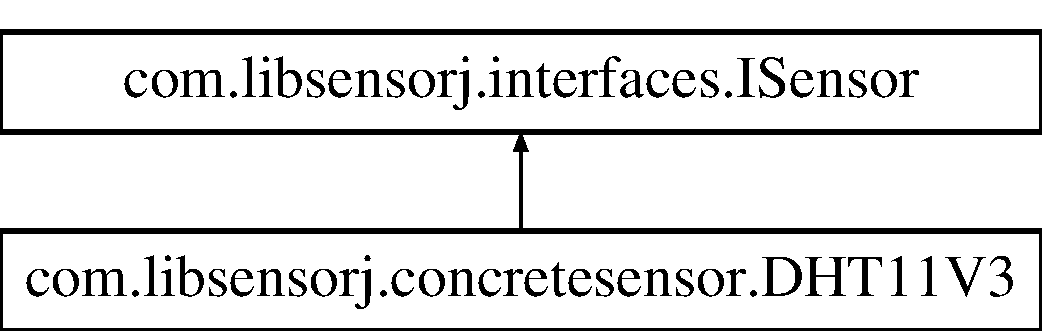
\includegraphics[height=2.000000cm]{classcom_1_1libsensorj_1_1concretesensor_1_1DHT11V3}
\end{center}
\end{figure}
\subsection*{Public Member Functions}
\begin{DoxyCompactItemize}
\item 
\hyperlink{classcom_1_1libsensorj_1_1concretesensor_1_1DHT11V3_a4996e16bdabeb71e35d8358a7e8248ca}{D\+H\+T11\+V3} ()
\item 
\hyperlink{classcom_1_1libsensorj_1_1concretesensor_1_1DHT11V3_a996dadcfe1bd20cd07d94be5c31b5453}{D\+H\+T11\+V3} (int pin)
\item 
\hyperlink{classcom_1_1libsensorj_1_1concretesensor_1_1DHT11V3_a1b40e6e4ec8ddd4df32c86d2dbe280b4}{D\+H\+T11\+V3} (Pin pin)
\item 
double \hyperlink{classcom_1_1libsensorj_1_1concretesensor_1_1DHT11V3_a15f5982dba996cc76bb7d0722ed70d31}{read\+Value} ()
\item 
synchronized double \hyperlink{classcom_1_1libsensorj_1_1concretesensor_1_1DHT11V3_afb1b93f01e2d40f12d9889217e5a37ee}{get\+Temperature\+In\+Celsius} ()
\item 
synchronized double \hyperlink{classcom_1_1libsensorj_1_1concretesensor_1_1DHT11V3_a7d1e369f920792870655add65dfed553}{get\+Temperature\+In\+Fahrenheit} ()
\item 
synchronized double \hyperlink{classcom_1_1libsensorj_1_1concretesensor_1_1DHT11V3_a3c8ecacf36b2b4d2de219dd9912b64b5}{get\+Temperature\+In\+Kelvin} ()
\item 
void \hyperlink{classcom_1_1libsensorj_1_1concretesensor_1_1DHT11V3_a94e402a3ea89ad3ee46725fdd64b4c82}{get\+Instance} ()
\end{DoxyCompactItemize}
\subsection*{Private Member Functions}
\begin{DoxyCompactItemize}
\item 
double \hyperlink{classcom_1_1libsensorj_1_1concretesensor_1_1DHT11V3_aba55ef9b04ccfa46d57079a526da9082}{get\+Temperature} (Temperature\+Scale from)
\end{DoxyCompactItemize}
\subsection*{Private Attributes}
\begin{DoxyCompactItemize}
\item 
int \hyperlink{classcom_1_1libsensorj_1_1concretesensor_1_1DHT11V3_a0c34b9cc559817c10910b1a6180decfd}{temperature}
\item 
Gpio\+Pin\+Digital\+Multipurpose \hyperlink{classcom_1_1libsensorj_1_1concretesensor_1_1DHT11V3_ab72b7b7ed1bd497e7b2818147afeeba9}{dht11\+Pin}
\end{DoxyCompactItemize}
\subsection*{Static Private Attributes}
\begin{DoxyCompactItemize}
\item 
static final Pin \hyperlink{classcom_1_1libsensorj_1_1concretesensor_1_1DHT11V3_a5abd2ea6b296cbd458df3e9170201913}{D\+E\+F\+A\+U\+L\+T\+\_\+\+P\+I\+N} = Raspi\+Pin.\+G\+P\+I\+O\+\_\+04
\item 
static final Logger \hyperlink{classcom_1_1libsensorj_1_1concretesensor_1_1DHT11V3_ac0cd3bfc7916b033ac50cebead5ba268}{L\+O\+G\+G\+E\+R}
\end{DoxyCompactItemize}


\subsection{Detailed Description}
The Class \hyperlink{classcom_1_1libsensorj_1_1concretesensor_1_1DHT11V3}{D\+H\+T11\+V3}. 

\subsection{Constructor \& Destructor Documentation}
\hypertarget{classcom_1_1libsensorj_1_1concretesensor_1_1DHT11V3_a4996e16bdabeb71e35d8358a7e8248ca}{}\index{com\+::libsensorj\+::concretesensor\+::\+D\+H\+T11\+V3@{com\+::libsensorj\+::concretesensor\+::\+D\+H\+T11\+V3}!D\+H\+T11\+V3@{D\+H\+T11\+V3}}
\index{D\+H\+T11\+V3@{D\+H\+T11\+V3}!com\+::libsensorj\+::concretesensor\+::\+D\+H\+T11\+V3@{com\+::libsensorj\+::concretesensor\+::\+D\+H\+T11\+V3}}
\subsubsection[{D\+H\+T11\+V3}]{\setlength{\rightskip}{0pt plus 5cm}com.\+libsensorj.\+concretesensor.\+D\+H\+T11\+V3.\+D\+H\+T11\+V3 (
\begin{DoxyParamCaption}
{}
\end{DoxyParamCaption}
)}\label{classcom_1_1libsensorj_1_1concretesensor_1_1DHT11V3_a4996e16bdabeb71e35d8358a7e8248ca}
Instantiates a new D\+Ht11 v3. \hypertarget{classcom_1_1libsensorj_1_1concretesensor_1_1DHT11V3_a996dadcfe1bd20cd07d94be5c31b5453}{}\index{com\+::libsensorj\+::concretesensor\+::\+D\+H\+T11\+V3@{com\+::libsensorj\+::concretesensor\+::\+D\+H\+T11\+V3}!D\+H\+T11\+V3@{D\+H\+T11\+V3}}
\index{D\+H\+T11\+V3@{D\+H\+T11\+V3}!com\+::libsensorj\+::concretesensor\+::\+D\+H\+T11\+V3@{com\+::libsensorj\+::concretesensor\+::\+D\+H\+T11\+V3}}
\subsubsection[{D\+H\+T11\+V3}]{\setlength{\rightskip}{0pt plus 5cm}com.\+libsensorj.\+concretesensor.\+D\+H\+T11\+V3.\+D\+H\+T11\+V3 (
\begin{DoxyParamCaption}
\item[{int}]{pin}
\end{DoxyParamCaption}
)}\label{classcom_1_1libsensorj_1_1concretesensor_1_1DHT11V3_a996dadcfe1bd20cd07d94be5c31b5453}
Instantiates a new D\+Ht11 v3.


\begin{DoxyParams}{Parameters}
{\em pin} & the pin \\
\hline
\end{DoxyParams}
\hypertarget{classcom_1_1libsensorj_1_1concretesensor_1_1DHT11V3_a1b40e6e4ec8ddd4df32c86d2dbe280b4}{}\index{com\+::libsensorj\+::concretesensor\+::\+D\+H\+T11\+V3@{com\+::libsensorj\+::concretesensor\+::\+D\+H\+T11\+V3}!D\+H\+T11\+V3@{D\+H\+T11\+V3}}
\index{D\+H\+T11\+V3@{D\+H\+T11\+V3}!com\+::libsensorj\+::concretesensor\+::\+D\+H\+T11\+V3@{com\+::libsensorj\+::concretesensor\+::\+D\+H\+T11\+V3}}
\subsubsection[{D\+H\+T11\+V3}]{\setlength{\rightskip}{0pt plus 5cm}com.\+libsensorj.\+concretesensor.\+D\+H\+T11\+V3.\+D\+H\+T11\+V3 (
\begin{DoxyParamCaption}
\item[{Pin}]{pin}
\end{DoxyParamCaption}
)}\label{classcom_1_1libsensorj_1_1concretesensor_1_1DHT11V3_a1b40e6e4ec8ddd4df32c86d2dbe280b4}
Instantiates a new D\+Ht11 v3.


\begin{DoxyParams}{Parameters}
{\em pin} & the pin \\
\hline
\end{DoxyParams}


\subsection{Member Function Documentation}
\hypertarget{classcom_1_1libsensorj_1_1concretesensor_1_1DHT11V3_a94e402a3ea89ad3ee46725fdd64b4c82}{}\index{com\+::libsensorj\+::concretesensor\+::\+D\+H\+T11\+V3@{com\+::libsensorj\+::concretesensor\+::\+D\+H\+T11\+V3}!get\+Instance@{get\+Instance}}
\index{get\+Instance@{get\+Instance}!com\+::libsensorj\+::concretesensor\+::\+D\+H\+T11\+V3@{com\+::libsensorj\+::concretesensor\+::\+D\+H\+T11\+V3}}
\subsubsection[{get\+Instance}]{\setlength{\rightskip}{0pt plus 5cm}void com.\+libsensorj.\+concretesensor.\+D\+H\+T11\+V3.\+get\+Instance (
\begin{DoxyParamCaption}
{}
\end{DoxyParamCaption}
)}\label{classcom_1_1libsensorj_1_1concretesensor_1_1DHT11V3_a94e402a3ea89ad3ee46725fdd64b4c82}
Gets the single instance of I\+Sensor.

\begin{DoxyReturn}{Returns}
single instance of I\+Sensor 
\end{DoxyReturn}


Implements \hyperlink{interfacecom_1_1libsensorj_1_1interfaces_1_1ISensor_a3c3db93a33adecde81a528651790f75e}{com.\+libsensorj.\+interfaces.\+I\+Sensor}.

\hypertarget{classcom_1_1libsensorj_1_1concretesensor_1_1DHT11V3_aba55ef9b04ccfa46d57079a526da9082}{}\index{com\+::libsensorj\+::concretesensor\+::\+D\+H\+T11\+V3@{com\+::libsensorj\+::concretesensor\+::\+D\+H\+T11\+V3}!get\+Temperature@{get\+Temperature}}
\index{get\+Temperature@{get\+Temperature}!com\+::libsensorj\+::concretesensor\+::\+D\+H\+T11\+V3@{com\+::libsensorj\+::concretesensor\+::\+D\+H\+T11\+V3}}
\subsubsection[{get\+Temperature}]{\setlength{\rightskip}{0pt plus 5cm}double com.\+libsensorj.\+concretesensor.\+D\+H\+T11\+V3.\+get\+Temperature (
\begin{DoxyParamCaption}
\item[{Temperature\+Scale}]{from}
\end{DoxyParamCaption}
)\hspace{0.3cm}{\ttfamily [private]}}\label{classcom_1_1libsensorj_1_1concretesensor_1_1DHT11V3_aba55ef9b04ccfa46d57079a526da9082}
Gets the temperature.


\begin{DoxyParams}{Parameters}
{\em from} & the Temperature\+Scale \\
\hline
\end{DoxyParams}
\begin{DoxyReturn}{Returns}
the temperature 
\end{DoxyReturn}
\hypertarget{classcom_1_1libsensorj_1_1concretesensor_1_1DHT11V3_afb1b93f01e2d40f12d9889217e5a37ee}{}\index{com\+::libsensorj\+::concretesensor\+::\+D\+H\+T11\+V3@{com\+::libsensorj\+::concretesensor\+::\+D\+H\+T11\+V3}!get\+Temperature\+In\+Celsius@{get\+Temperature\+In\+Celsius}}
\index{get\+Temperature\+In\+Celsius@{get\+Temperature\+In\+Celsius}!com\+::libsensorj\+::concretesensor\+::\+D\+H\+T11\+V3@{com\+::libsensorj\+::concretesensor\+::\+D\+H\+T11\+V3}}
\subsubsection[{get\+Temperature\+In\+Celsius}]{\setlength{\rightskip}{0pt plus 5cm}synchronized double com.\+libsensorj.\+concretesensor.\+D\+H\+T11\+V3.\+get\+Temperature\+In\+Celsius (
\begin{DoxyParamCaption}
{}
\end{DoxyParamCaption}
)}\label{classcom_1_1libsensorj_1_1concretesensor_1_1DHT11V3_afb1b93f01e2d40f12d9889217e5a37ee}
Gets the temperature in celsius.

\begin{DoxyReturn}{Returns}
the temperature in celsius 
\end{DoxyReturn}
\hypertarget{classcom_1_1libsensorj_1_1concretesensor_1_1DHT11V3_a7d1e369f920792870655add65dfed553}{}\index{com\+::libsensorj\+::concretesensor\+::\+D\+H\+T11\+V3@{com\+::libsensorj\+::concretesensor\+::\+D\+H\+T11\+V3}!get\+Temperature\+In\+Fahrenheit@{get\+Temperature\+In\+Fahrenheit}}
\index{get\+Temperature\+In\+Fahrenheit@{get\+Temperature\+In\+Fahrenheit}!com\+::libsensorj\+::concretesensor\+::\+D\+H\+T11\+V3@{com\+::libsensorj\+::concretesensor\+::\+D\+H\+T11\+V3}}
\subsubsection[{get\+Temperature\+In\+Fahrenheit}]{\setlength{\rightskip}{0pt plus 5cm}synchronized double com.\+libsensorj.\+concretesensor.\+D\+H\+T11\+V3.\+get\+Temperature\+In\+Fahrenheit (
\begin{DoxyParamCaption}
{}
\end{DoxyParamCaption}
)}\label{classcom_1_1libsensorj_1_1concretesensor_1_1DHT11V3_a7d1e369f920792870655add65dfed553}
Gets the temperature in fahrenheit.

\begin{DoxyReturn}{Returns}
the temperature in fahrenheit 
\end{DoxyReturn}
\hypertarget{classcom_1_1libsensorj_1_1concretesensor_1_1DHT11V3_a3c8ecacf36b2b4d2de219dd9912b64b5}{}\index{com\+::libsensorj\+::concretesensor\+::\+D\+H\+T11\+V3@{com\+::libsensorj\+::concretesensor\+::\+D\+H\+T11\+V3}!get\+Temperature\+In\+Kelvin@{get\+Temperature\+In\+Kelvin}}
\index{get\+Temperature\+In\+Kelvin@{get\+Temperature\+In\+Kelvin}!com\+::libsensorj\+::concretesensor\+::\+D\+H\+T11\+V3@{com\+::libsensorj\+::concretesensor\+::\+D\+H\+T11\+V3}}
\subsubsection[{get\+Temperature\+In\+Kelvin}]{\setlength{\rightskip}{0pt plus 5cm}synchronized double com.\+libsensorj.\+concretesensor.\+D\+H\+T11\+V3.\+get\+Temperature\+In\+Kelvin (
\begin{DoxyParamCaption}
{}
\end{DoxyParamCaption}
)}\label{classcom_1_1libsensorj_1_1concretesensor_1_1DHT11V3_a3c8ecacf36b2b4d2de219dd9912b64b5}
Gets the temperature in kelvin.

\begin{DoxyReturn}{Returns}
the temperature in kelvin 
\end{DoxyReturn}
\hypertarget{classcom_1_1libsensorj_1_1concretesensor_1_1DHT11V3_a15f5982dba996cc76bb7d0722ed70d31}{}\index{com\+::libsensorj\+::concretesensor\+::\+D\+H\+T11\+V3@{com\+::libsensorj\+::concretesensor\+::\+D\+H\+T11\+V3}!read\+Value@{read\+Value}}
\index{read\+Value@{read\+Value}!com\+::libsensorj\+::concretesensor\+::\+D\+H\+T11\+V3@{com\+::libsensorj\+::concretesensor\+::\+D\+H\+T11\+V3}}
\subsubsection[{read\+Value}]{\setlength{\rightskip}{0pt plus 5cm}double com.\+libsensorj.\+concretesensor.\+D\+H\+T11\+V3.\+read\+Value (
\begin{DoxyParamCaption}
{}
\end{DoxyParamCaption}
)}\label{classcom_1_1libsensorj_1_1concretesensor_1_1DHT11V3_a15f5982dba996cc76bb7d0722ed70d31}
Read value.

\begin{DoxyReturn}{Returns}
the value readed 
\end{DoxyReturn}


\subsection{Member Data Documentation}
\hypertarget{classcom_1_1libsensorj_1_1concretesensor_1_1DHT11V3_a5abd2ea6b296cbd458df3e9170201913}{}\index{com\+::libsensorj\+::concretesensor\+::\+D\+H\+T11\+V3@{com\+::libsensorj\+::concretesensor\+::\+D\+H\+T11\+V3}!D\+E\+F\+A\+U\+L\+T\+\_\+\+P\+I\+N@{D\+E\+F\+A\+U\+L\+T\+\_\+\+P\+I\+N}}
\index{D\+E\+F\+A\+U\+L\+T\+\_\+\+P\+I\+N@{D\+E\+F\+A\+U\+L\+T\+\_\+\+P\+I\+N}!com\+::libsensorj\+::concretesensor\+::\+D\+H\+T11\+V3@{com\+::libsensorj\+::concretesensor\+::\+D\+H\+T11\+V3}}
\subsubsection[{D\+E\+F\+A\+U\+L\+T\+\_\+\+P\+I\+N}]{\setlength{\rightskip}{0pt plus 5cm}final Pin com.\+libsensorj.\+concretesensor.\+D\+H\+T11\+V3.\+D\+E\+F\+A\+U\+L\+T\+\_\+\+P\+I\+N = Raspi\+Pin.\+G\+P\+I\+O\+\_\+04\hspace{0.3cm}{\ttfamily [static]}, {\ttfamily [private]}}\label{classcom_1_1libsensorj_1_1concretesensor_1_1DHT11V3_a5abd2ea6b296cbd458df3e9170201913}
The Constant D\+E\+F\+A\+U\+L\+T\+\_\+\+P\+I\+N. \hypertarget{classcom_1_1libsensorj_1_1concretesensor_1_1DHT11V3_ab72b7b7ed1bd497e7b2818147afeeba9}{}\index{com\+::libsensorj\+::concretesensor\+::\+D\+H\+T11\+V3@{com\+::libsensorj\+::concretesensor\+::\+D\+H\+T11\+V3}!dht11\+Pin@{dht11\+Pin}}
\index{dht11\+Pin@{dht11\+Pin}!com\+::libsensorj\+::concretesensor\+::\+D\+H\+T11\+V3@{com\+::libsensorj\+::concretesensor\+::\+D\+H\+T11\+V3}}
\subsubsection[{dht11\+Pin}]{\setlength{\rightskip}{0pt plus 5cm}Gpio\+Pin\+Digital\+Multipurpose com.\+libsensorj.\+concretesensor.\+D\+H\+T11\+V3.\+dht11\+Pin\hspace{0.3cm}{\ttfamily [private]}}\label{classcom_1_1libsensorj_1_1concretesensor_1_1DHT11V3_ab72b7b7ed1bd497e7b2818147afeeba9}
The dht11 pin. \hypertarget{classcom_1_1libsensorj_1_1concretesensor_1_1DHT11V3_ac0cd3bfc7916b033ac50cebead5ba268}{}\index{com\+::libsensorj\+::concretesensor\+::\+D\+H\+T11\+V3@{com\+::libsensorj\+::concretesensor\+::\+D\+H\+T11\+V3}!L\+O\+G\+G\+E\+R@{L\+O\+G\+G\+E\+R}}
\index{L\+O\+G\+G\+E\+R@{L\+O\+G\+G\+E\+R}!com\+::libsensorj\+::concretesensor\+::\+D\+H\+T11\+V3@{com\+::libsensorj\+::concretesensor\+::\+D\+H\+T11\+V3}}
\subsubsection[{L\+O\+G\+G\+E\+R}]{\setlength{\rightskip}{0pt plus 5cm}final Logger com.\+libsensorj.\+concretesensor.\+D\+H\+T11\+V3.\+L\+O\+G\+G\+E\+R\hspace{0.3cm}{\ttfamily [static]}, {\ttfamily [private]}}\label{classcom_1_1libsensorj_1_1concretesensor_1_1DHT11V3_ac0cd3bfc7916b033ac50cebead5ba268}
{\bfseries Initial value\+:}
\begin{DoxyCode}
= LogManager.getLogger(\hyperlink{classcom_1_1libsensorj_1_1concretesensor_1_1DHT11V3_a4996e16bdabeb71e35d8358a7e8248ca}{DHT11V3}.class
            .getName())
\end{DoxyCode}
The Constant L\+O\+G\+G\+E\+R. \hypertarget{classcom_1_1libsensorj_1_1concretesensor_1_1DHT11V3_a0c34b9cc559817c10910b1a6180decfd}{}\index{com\+::libsensorj\+::concretesensor\+::\+D\+H\+T11\+V3@{com\+::libsensorj\+::concretesensor\+::\+D\+H\+T11\+V3}!temperature@{temperature}}
\index{temperature@{temperature}!com\+::libsensorj\+::concretesensor\+::\+D\+H\+T11\+V3@{com\+::libsensorj\+::concretesensor\+::\+D\+H\+T11\+V3}}
\subsubsection[{temperature}]{\setlength{\rightskip}{0pt plus 5cm}int com.\+libsensorj.\+concretesensor.\+D\+H\+T11\+V3.\+temperature\hspace{0.3cm}{\ttfamily [private]}}\label{classcom_1_1libsensorj_1_1concretesensor_1_1DHT11V3_a0c34b9cc559817c10910b1a6180decfd}
The temperature. 

The documentation for this class was generated from the following file\+:\begin{DoxyCompactItemize}
\item 
main/java/com/libsensorj/concretesensor/\hyperlink{DHT11V3_8java}{D\+H\+T11\+V3.\+java}\end{DoxyCompactItemize}

\hypertarget{classcom_1_1libsensorj_1_1examples_1_1DHT11V3Example}{}\section{com.\+libsensorj.\+examples.\+D\+H\+T11\+V3\+Example Class Reference}
\label{classcom_1_1libsensorj_1_1examples_1_1DHT11V3Example}\index{com.\+libsensorj.\+examples.\+D\+H\+T11\+V3\+Example@{com.\+libsensorj.\+examples.\+D\+H\+T11\+V3\+Example}}
\subsection*{Static Public Member Functions}
\begin{DoxyCompactItemize}
\item 
static void \hyperlink{classcom_1_1libsensorj_1_1examples_1_1DHT11V3Example_a4ed6af58ddd7026d7ca95b0195683cfb}{main} (String\mbox{[}$\,$\mbox{]} args)
\end{DoxyCompactItemize}
\subsection*{Static Private Attributes}
\begin{DoxyCompactItemize}
\item 
static \hyperlink{interfacecom_1_1libsensorj_1_1interfaces_1_1ISensor}{I\+Sensor} \hyperlink{classcom_1_1libsensorj_1_1examples_1_1DHT11V3Example_abb6525b581e1d2e3cdc9d5904f0bd69d}{dht11}
\item 
static final Logger \hyperlink{classcom_1_1libsensorj_1_1examples_1_1DHT11V3Example_a8bce3e00742905abcf18e77164a69279}{L\+O\+G\+G\+E\+R}
\end{DoxyCompactItemize}


\subsection{Detailed Description}
The Class \hyperlink{classcom_1_1libsensorj_1_1examples_1_1DHT11V3Example}{D\+H\+T11\+V3\+Example}. 

\subsection{Member Function Documentation}
\hypertarget{classcom_1_1libsensorj_1_1examples_1_1DHT11V3Example_a4ed6af58ddd7026d7ca95b0195683cfb}{}\index{com\+::libsensorj\+::examples\+::\+D\+H\+T11\+V3\+Example@{com\+::libsensorj\+::examples\+::\+D\+H\+T11\+V3\+Example}!main@{main}}
\index{main@{main}!com\+::libsensorj\+::examples\+::\+D\+H\+T11\+V3\+Example@{com\+::libsensorj\+::examples\+::\+D\+H\+T11\+V3\+Example}}
\subsubsection[{main}]{\setlength{\rightskip}{0pt plus 5cm}static void com.\+libsensorj.\+examples.\+D\+H\+T11\+V3\+Example.\+main (
\begin{DoxyParamCaption}
\item[{String\mbox{[}$\,$\mbox{]}}]{args}
\end{DoxyParamCaption}
)\hspace{0.3cm}{\ttfamily [static]}}\label{classcom_1_1libsensorj_1_1examples_1_1DHT11V3Example_a4ed6af58ddd7026d7ca95b0195683cfb}
The main method.


\begin{DoxyParams}{Parameters}
{\em args} & the arguments \\
\hline
\end{DoxyParams}


\subsection{Member Data Documentation}
\hypertarget{classcom_1_1libsensorj_1_1examples_1_1DHT11V3Example_abb6525b581e1d2e3cdc9d5904f0bd69d}{}\index{com\+::libsensorj\+::examples\+::\+D\+H\+T11\+V3\+Example@{com\+::libsensorj\+::examples\+::\+D\+H\+T11\+V3\+Example}!dht11@{dht11}}
\index{dht11@{dht11}!com\+::libsensorj\+::examples\+::\+D\+H\+T11\+V3\+Example@{com\+::libsensorj\+::examples\+::\+D\+H\+T11\+V3\+Example}}
\subsubsection[{dht11}]{\setlength{\rightskip}{0pt plus 5cm}{\bf I\+Sensor} com.\+libsensorj.\+examples.\+D\+H\+T11\+V3\+Example.\+dht11\hspace{0.3cm}{\ttfamily [static]}, {\ttfamily [private]}}\label{classcom_1_1libsensorj_1_1examples_1_1DHT11V3Example_abb6525b581e1d2e3cdc9d5904f0bd69d}
The I\+Sensor dht11. \hypertarget{classcom_1_1libsensorj_1_1examples_1_1DHT11V3Example_a8bce3e00742905abcf18e77164a69279}{}\index{com\+::libsensorj\+::examples\+::\+D\+H\+T11\+V3\+Example@{com\+::libsensorj\+::examples\+::\+D\+H\+T11\+V3\+Example}!L\+O\+G\+G\+E\+R@{L\+O\+G\+G\+E\+R}}
\index{L\+O\+G\+G\+E\+R@{L\+O\+G\+G\+E\+R}!com\+::libsensorj\+::examples\+::\+D\+H\+T11\+V3\+Example@{com\+::libsensorj\+::examples\+::\+D\+H\+T11\+V3\+Example}}
\subsubsection[{L\+O\+G\+G\+E\+R}]{\setlength{\rightskip}{0pt plus 5cm}final Logger com.\+libsensorj.\+examples.\+D\+H\+T11\+V3\+Example.\+L\+O\+G\+G\+E\+R\hspace{0.3cm}{\ttfamily [static]}, {\ttfamily [private]}}\label{classcom_1_1libsensorj_1_1examples_1_1DHT11V3Example_a8bce3e00742905abcf18e77164a69279}
{\bfseries Initial value\+:}
\begin{DoxyCode}
= LogManager
            .getLogger(DHT11TemperatureExample.class.getName())
\end{DoxyCode}
The Constant L\+O\+G\+G\+E\+R. 

The documentation for this class was generated from the following file\+:\begin{DoxyCompactItemize}
\item 
main/java/com/libsensorj/examples/\hyperlink{DHT11V3Example_8java}{D\+H\+T11\+V3\+Example.\+java}\end{DoxyCompactItemize}

\hypertarget{classcom_1_1libsensorj_1_1concretefactory_1_1DHT11V3Factory}{}\section{com.\+libsensorj.\+concretefactory.\+D\+H\+T11\+V3\+Factory Class Reference}
\label{classcom_1_1libsensorj_1_1concretefactory_1_1DHT11V3Factory}\index{com.\+libsensorj.\+concretefactory.\+D\+H\+T11\+V3\+Factory@{com.\+libsensorj.\+concretefactory.\+D\+H\+T11\+V3\+Factory}}
Inheritance diagram for com.\+libsensorj.\+concretefactory.\+D\+H\+T11\+V3\+Factory\+:\begin{figure}[H]
\begin{center}
\leavevmode
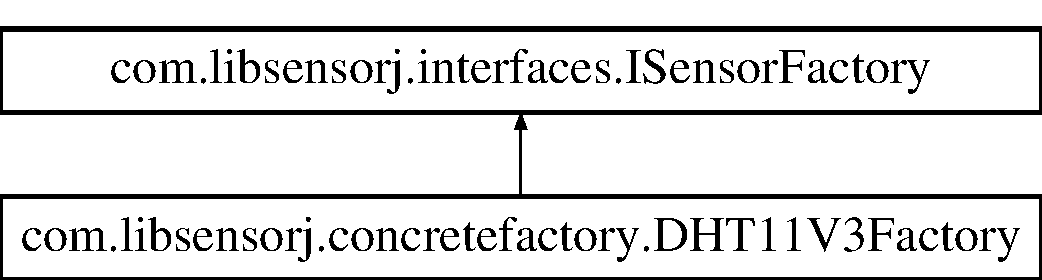
\includegraphics[height=2.000000cm]{classcom_1_1libsensorj_1_1concretefactory_1_1DHT11V3Factory}
\end{center}
\end{figure}
\subsection*{Public Member Functions}
\begin{DoxyCompactItemize}
\item 
\hyperlink{interfacecom_1_1libsensorj_1_1interfaces_1_1ISensor}{I\+Sensor} \hyperlink{classcom_1_1libsensorj_1_1concretefactory_1_1DHT11V3Factory_ad89c967025d654490729d2f69438805e}{create\+Sensor} ()
\item 
\hyperlink{classcom_1_1libsensorj_1_1interfaces_1_1IEvent}{I\+Event} \hyperlink{classcom_1_1libsensorj_1_1concretefactory_1_1DHT11V3Factory_a7621f6dc5c877e6dfb160f68e50fd319}{create\+Event} ()
\end{DoxyCompactItemize}


\subsection{Detailed Description}
A factory for creating D\+H\+T11\+V3 objects. 

\subsection{Member Function Documentation}
\hypertarget{classcom_1_1libsensorj_1_1concretefactory_1_1DHT11V3Factory_a7621f6dc5c877e6dfb160f68e50fd319}{}\index{com\+::libsensorj\+::concretefactory\+::\+D\+H\+T11\+V3\+Factory@{com\+::libsensorj\+::concretefactory\+::\+D\+H\+T11\+V3\+Factory}!create\+Event@{create\+Event}}
\index{create\+Event@{create\+Event}!com\+::libsensorj\+::concretefactory\+::\+D\+H\+T11\+V3\+Factory@{com\+::libsensorj\+::concretefactory\+::\+D\+H\+T11\+V3\+Factory}}
\subsubsection[{create\+Event}]{\setlength{\rightskip}{0pt plus 5cm}{\bf I\+Event} com.\+libsensorj.\+concretefactory.\+D\+H\+T11\+V3\+Factory.\+create\+Event (
\begin{DoxyParamCaption}
{}
\end{DoxyParamCaption}
)}\label{classcom_1_1libsensorj_1_1concretefactory_1_1DHT11V3Factory_a7621f6dc5c877e6dfb160f68e50fd319}
Creates a new I\+Event object.

\begin{DoxyReturn}{Returns}
the I\+Event 
\end{DoxyReturn}


Implements \hyperlink{interfacecom_1_1libsensorj_1_1interfaces_1_1ISensorFactory_a2b074d01287a4e64677097255ba9e768}{com.\+libsensorj.\+interfaces.\+I\+Sensor\+Factory}.

\hypertarget{classcom_1_1libsensorj_1_1concretefactory_1_1DHT11V3Factory_ad89c967025d654490729d2f69438805e}{}\index{com\+::libsensorj\+::concretefactory\+::\+D\+H\+T11\+V3\+Factory@{com\+::libsensorj\+::concretefactory\+::\+D\+H\+T11\+V3\+Factory}!create\+Sensor@{create\+Sensor}}
\index{create\+Sensor@{create\+Sensor}!com\+::libsensorj\+::concretefactory\+::\+D\+H\+T11\+V3\+Factory@{com\+::libsensorj\+::concretefactory\+::\+D\+H\+T11\+V3\+Factory}}
\subsubsection[{create\+Sensor}]{\setlength{\rightskip}{0pt plus 5cm}{\bf I\+Sensor} com.\+libsensorj.\+concretefactory.\+D\+H\+T11\+V3\+Factory.\+create\+Sensor (
\begin{DoxyParamCaption}
{}
\end{DoxyParamCaption}
)}\label{classcom_1_1libsensorj_1_1concretefactory_1_1DHT11V3Factory_ad89c967025d654490729d2f69438805e}
Creates a new I\+Sensor object.

\begin{DoxyReturn}{Returns}
the I\+Sensor 
\end{DoxyReturn}


Implements \hyperlink{interfacecom_1_1libsensorj_1_1interfaces_1_1ISensorFactory_ac14c6d566c37c6a79c6db1e85634f25d}{com.\+libsensorj.\+interfaces.\+I\+Sensor\+Factory}.



The documentation for this class was generated from the following file\+:\begin{DoxyCompactItemize}
\item 
main/java/com/libsensorj/concretefactory/\hyperlink{DHT11V3Factory_8java}{D\+H\+T11\+V3\+Factory.\+java}\end{DoxyCompactItemize}

\hypertarget{classcom_1_1libsensorj_1_1concretesensor_1_1test_1_1DHT11V3Tests}{}\section{com.\+libsensorj.\+concretesensor.\+test.\+D\+H\+T11\+V3\+Tests Class Reference}
\label{classcom_1_1libsensorj_1_1concretesensor_1_1test_1_1DHT11V3Tests}\index{com.\+libsensorj.\+concretesensor.\+test.\+D\+H\+T11\+V3\+Tests@{com.\+libsensorj.\+concretesensor.\+test.\+D\+H\+T11\+V3\+Tests}}
\subsection*{Public Member Functions}
\begin{DoxyCompactItemize}
\item 
void \hyperlink{classcom_1_1libsensorj_1_1concretesensor_1_1test_1_1DHT11V3Tests_ab3427bd3d108c922dd65f661a2163cbd}{test\+Pin\+Provisioned} ()
\item 
void \hyperlink{classcom_1_1libsensorj_1_1concretesensor_1_1test_1_1DHT11V3Tests_ab3d399c94618aa2743dde25e5562cd9b}{test\+Get\+Temperature\+In\+Celsius} ()
\item 
void \hyperlink{classcom_1_1libsensorj_1_1concretesensor_1_1test_1_1DHT11V3Tests_ae9c538bf56fb20f9ee038b2aafdfd308}{test\+Get\+Temperature\+In\+Fahrenheit} ()
\item 
void \hyperlink{classcom_1_1libsensorj_1_1concretesensor_1_1test_1_1DHT11V3Tests_a054d8adbb80ae717587f1a572d2c4954}{test\+Get\+Temperature\+In\+Kelvin} ()
\end{DoxyCompactItemize}
\subsection*{Static Public Member Functions}
\begin{DoxyCompactItemize}
\item 
static void \hyperlink{classcom_1_1libsensorj_1_1concretesensor_1_1test_1_1DHT11V3Tests_a825eabc3f80c23c602ce09fc99b1b277}{setup} ()
\end{DoxyCompactItemize}
\subsection*{Static Private Attributes}
\begin{DoxyCompactItemize}
\item 
static Gpio\+Controller \hyperlink{classcom_1_1libsensorj_1_1concretesensor_1_1test_1_1DHT11V3Tests_a21c4675809d99d4752ae63d03d6bc519}{gpio}
\item 
static Gpio\+Pin\+Digital\+Input \hyperlink{classcom_1_1libsensorj_1_1concretesensor_1_1test_1_1DHT11V3Tests_aa313c38ed46c638515f7f43b5458f728}{pin}
\item 
static Pin\+State \hyperlink{classcom_1_1libsensorj_1_1concretesensor_1_1test_1_1DHT11V3Tests_a326b78365c6bfa39eea9b86c28a6b780}{pin\+Monitored\+State}
\item 
static final double \hyperlink{classcom_1_1libsensorj_1_1concretesensor_1_1test_1_1DHT11V3Tests_a2f2801f413ed01cd67cb5acf6cce2d80}{D\+A\+T\+A\+\_\+\+R\+E\+A\+D\+E\+D} = 29
\item 
static final String \hyperlink{classcom_1_1libsensorj_1_1concretesensor_1_1test_1_1DHT11V3Tests_abe087b3362924a1e965cf433b504d948}{R\+E\+A\+D\+V\+A\+L\+U\+E\+\_\+\+M\+E\+T\+H\+O\+D} = \char`\"{}read\+Value\char`\"{}
\item 
static final Logger \hyperlink{classcom_1_1libsensorj_1_1concretesensor_1_1test_1_1DHT11V3Tests_a1520ba3dc702c464bb28690691848a0a}{L\+O\+G\+G\+E\+R}
\end{DoxyCompactItemize}


\subsection{Detailed Description}
The Class \hyperlink{classcom_1_1libsensorj_1_1concretesensor_1_1test_1_1DHT11V3Tests}{D\+H\+T11\+V3\+Tests}. 

\subsection{Member Function Documentation}
\hypertarget{classcom_1_1libsensorj_1_1concretesensor_1_1test_1_1DHT11V3Tests_a825eabc3f80c23c602ce09fc99b1b277}{}\index{com\+::libsensorj\+::concretesensor\+::test\+::\+D\+H\+T11\+V3\+Tests@{com\+::libsensorj\+::concretesensor\+::test\+::\+D\+H\+T11\+V3\+Tests}!setup@{setup}}
\index{setup@{setup}!com\+::libsensorj\+::concretesensor\+::test\+::\+D\+H\+T11\+V3\+Tests@{com\+::libsensorj\+::concretesensor\+::test\+::\+D\+H\+T11\+V3\+Tests}}
\subsubsection[{setup}]{\setlength{\rightskip}{0pt plus 5cm}static void com.\+libsensorj.\+concretesensor.\+test.\+D\+H\+T11\+V3\+Tests.\+setup (
\begin{DoxyParamCaption}
{}
\end{DoxyParamCaption}
)\hspace{0.3cm}{\ttfamily [static]}}\label{classcom_1_1libsensorj_1_1concretesensor_1_1test_1_1DHT11V3Tests_a825eabc3f80c23c602ce09fc99b1b277}
Setup. \hypertarget{classcom_1_1libsensorj_1_1concretesensor_1_1test_1_1DHT11V3Tests_ab3d399c94618aa2743dde25e5562cd9b}{}\index{com\+::libsensorj\+::concretesensor\+::test\+::\+D\+H\+T11\+V3\+Tests@{com\+::libsensorj\+::concretesensor\+::test\+::\+D\+H\+T11\+V3\+Tests}!test\+Get\+Temperature\+In\+Celsius@{test\+Get\+Temperature\+In\+Celsius}}
\index{test\+Get\+Temperature\+In\+Celsius@{test\+Get\+Temperature\+In\+Celsius}!com\+::libsensorj\+::concretesensor\+::test\+::\+D\+H\+T11\+V3\+Tests@{com\+::libsensorj\+::concretesensor\+::test\+::\+D\+H\+T11\+V3\+Tests}}
\subsubsection[{test\+Get\+Temperature\+In\+Celsius}]{\setlength{\rightskip}{0pt plus 5cm}void com.\+libsensorj.\+concretesensor.\+test.\+D\+H\+T11\+V3\+Tests.\+test\+Get\+Temperature\+In\+Celsius (
\begin{DoxyParamCaption}
{}
\end{DoxyParamCaption}
)}\label{classcom_1_1libsensorj_1_1concretesensor_1_1test_1_1DHT11V3Tests_ab3d399c94618aa2743dde25e5562cd9b}
Test Get\+Temperature\+In\+Celsius. \hypertarget{classcom_1_1libsensorj_1_1concretesensor_1_1test_1_1DHT11V3Tests_ae9c538bf56fb20f9ee038b2aafdfd308}{}\index{com\+::libsensorj\+::concretesensor\+::test\+::\+D\+H\+T11\+V3\+Tests@{com\+::libsensorj\+::concretesensor\+::test\+::\+D\+H\+T11\+V3\+Tests}!test\+Get\+Temperature\+In\+Fahrenheit@{test\+Get\+Temperature\+In\+Fahrenheit}}
\index{test\+Get\+Temperature\+In\+Fahrenheit@{test\+Get\+Temperature\+In\+Fahrenheit}!com\+::libsensorj\+::concretesensor\+::test\+::\+D\+H\+T11\+V3\+Tests@{com\+::libsensorj\+::concretesensor\+::test\+::\+D\+H\+T11\+V3\+Tests}}
\subsubsection[{test\+Get\+Temperature\+In\+Fahrenheit}]{\setlength{\rightskip}{0pt plus 5cm}void com.\+libsensorj.\+concretesensor.\+test.\+D\+H\+T11\+V3\+Tests.\+test\+Get\+Temperature\+In\+Fahrenheit (
\begin{DoxyParamCaption}
{}
\end{DoxyParamCaption}
)}\label{classcom_1_1libsensorj_1_1concretesensor_1_1test_1_1DHT11V3Tests_ae9c538bf56fb20f9ee038b2aafdfd308}
Test Get\+Temperature\+In\+Fahrenheit. \hypertarget{classcom_1_1libsensorj_1_1concretesensor_1_1test_1_1DHT11V3Tests_a054d8adbb80ae717587f1a572d2c4954}{}\index{com\+::libsensorj\+::concretesensor\+::test\+::\+D\+H\+T11\+V3\+Tests@{com\+::libsensorj\+::concretesensor\+::test\+::\+D\+H\+T11\+V3\+Tests}!test\+Get\+Temperature\+In\+Kelvin@{test\+Get\+Temperature\+In\+Kelvin}}
\index{test\+Get\+Temperature\+In\+Kelvin@{test\+Get\+Temperature\+In\+Kelvin}!com\+::libsensorj\+::concretesensor\+::test\+::\+D\+H\+T11\+V3\+Tests@{com\+::libsensorj\+::concretesensor\+::test\+::\+D\+H\+T11\+V3\+Tests}}
\subsubsection[{test\+Get\+Temperature\+In\+Kelvin}]{\setlength{\rightskip}{0pt plus 5cm}void com.\+libsensorj.\+concretesensor.\+test.\+D\+H\+T11\+V3\+Tests.\+test\+Get\+Temperature\+In\+Kelvin (
\begin{DoxyParamCaption}
{}
\end{DoxyParamCaption}
)}\label{classcom_1_1libsensorj_1_1concretesensor_1_1test_1_1DHT11V3Tests_a054d8adbb80ae717587f1a572d2c4954}
Test Get\+Temperature\+In\+Kelvin. \hypertarget{classcom_1_1libsensorj_1_1concretesensor_1_1test_1_1DHT11V3Tests_ab3427bd3d108c922dd65f661a2163cbd}{}\index{com\+::libsensorj\+::concretesensor\+::test\+::\+D\+H\+T11\+V3\+Tests@{com\+::libsensorj\+::concretesensor\+::test\+::\+D\+H\+T11\+V3\+Tests}!test\+Pin\+Provisioned@{test\+Pin\+Provisioned}}
\index{test\+Pin\+Provisioned@{test\+Pin\+Provisioned}!com\+::libsensorj\+::concretesensor\+::test\+::\+D\+H\+T11\+V3\+Tests@{com\+::libsensorj\+::concretesensor\+::test\+::\+D\+H\+T11\+V3\+Tests}}
\subsubsection[{test\+Pin\+Provisioned}]{\setlength{\rightskip}{0pt plus 5cm}void com.\+libsensorj.\+concretesensor.\+test.\+D\+H\+T11\+V3\+Tests.\+test\+Pin\+Provisioned (
\begin{DoxyParamCaption}
{}
\end{DoxyParamCaption}
)}\label{classcom_1_1libsensorj_1_1concretesensor_1_1test_1_1DHT11V3Tests_ab3427bd3d108c922dd65f661a2163cbd}
Test pin provisioned. 

\subsection{Member Data Documentation}
\hypertarget{classcom_1_1libsensorj_1_1concretesensor_1_1test_1_1DHT11V3Tests_a2f2801f413ed01cd67cb5acf6cce2d80}{}\index{com\+::libsensorj\+::concretesensor\+::test\+::\+D\+H\+T11\+V3\+Tests@{com\+::libsensorj\+::concretesensor\+::test\+::\+D\+H\+T11\+V3\+Tests}!D\+A\+T\+A\+\_\+\+R\+E\+A\+D\+E\+D@{D\+A\+T\+A\+\_\+\+R\+E\+A\+D\+E\+D}}
\index{D\+A\+T\+A\+\_\+\+R\+E\+A\+D\+E\+D@{D\+A\+T\+A\+\_\+\+R\+E\+A\+D\+E\+D}!com\+::libsensorj\+::concretesensor\+::test\+::\+D\+H\+T11\+V3\+Tests@{com\+::libsensorj\+::concretesensor\+::test\+::\+D\+H\+T11\+V3\+Tests}}
\subsubsection[{D\+A\+T\+A\+\_\+\+R\+E\+A\+D\+E\+D}]{\setlength{\rightskip}{0pt plus 5cm}final double com.\+libsensorj.\+concretesensor.\+test.\+D\+H\+T11\+V3\+Tests.\+D\+A\+T\+A\+\_\+\+R\+E\+A\+D\+E\+D = 29\hspace{0.3cm}{\ttfamily [static]}, {\ttfamily [private]}}\label{classcom_1_1libsensorj_1_1concretesensor_1_1test_1_1DHT11V3Tests_a2f2801f413ed01cd67cb5acf6cce2d80}
The Constant D\+A\+T\+A\+\_\+\+R\+E\+A\+D\+E\+D. \hypertarget{classcom_1_1libsensorj_1_1concretesensor_1_1test_1_1DHT11V3Tests_a21c4675809d99d4752ae63d03d6bc519}{}\index{com\+::libsensorj\+::concretesensor\+::test\+::\+D\+H\+T11\+V3\+Tests@{com\+::libsensorj\+::concretesensor\+::test\+::\+D\+H\+T11\+V3\+Tests}!gpio@{gpio}}
\index{gpio@{gpio}!com\+::libsensorj\+::concretesensor\+::test\+::\+D\+H\+T11\+V3\+Tests@{com\+::libsensorj\+::concretesensor\+::test\+::\+D\+H\+T11\+V3\+Tests}}
\subsubsection[{gpio}]{\setlength{\rightskip}{0pt plus 5cm}Gpio\+Controller com.\+libsensorj.\+concretesensor.\+test.\+D\+H\+T11\+V3\+Tests.\+gpio\hspace{0.3cm}{\ttfamily [static]}, {\ttfamily [private]}}\label{classcom_1_1libsensorj_1_1concretesensor_1_1test_1_1DHT11V3Tests_a21c4675809d99d4752ae63d03d6bc519}
The provider. The gpio. \hypertarget{classcom_1_1libsensorj_1_1concretesensor_1_1test_1_1DHT11V3Tests_a1520ba3dc702c464bb28690691848a0a}{}\index{com\+::libsensorj\+::concretesensor\+::test\+::\+D\+H\+T11\+V3\+Tests@{com\+::libsensorj\+::concretesensor\+::test\+::\+D\+H\+T11\+V3\+Tests}!L\+O\+G\+G\+E\+R@{L\+O\+G\+G\+E\+R}}
\index{L\+O\+G\+G\+E\+R@{L\+O\+G\+G\+E\+R}!com\+::libsensorj\+::concretesensor\+::test\+::\+D\+H\+T11\+V3\+Tests@{com\+::libsensorj\+::concretesensor\+::test\+::\+D\+H\+T11\+V3\+Tests}}
\subsubsection[{L\+O\+G\+G\+E\+R}]{\setlength{\rightskip}{0pt plus 5cm}final Logger com.\+libsensorj.\+concretesensor.\+test.\+D\+H\+T11\+V3\+Tests.\+L\+O\+G\+G\+E\+R\hspace{0.3cm}{\ttfamily [static]}, {\ttfamily [private]}}\label{classcom_1_1libsensorj_1_1concretesensor_1_1test_1_1DHT11V3Tests_a1520ba3dc702c464bb28690691848a0a}
{\bfseries Initial value\+:}
\begin{DoxyCode}
= LogManager
            .getLogger(DHT11V3Tests.class.getName())
\end{DoxyCode}
The Constant L\+O\+G\+G\+E\+R. \hypertarget{classcom_1_1libsensorj_1_1concretesensor_1_1test_1_1DHT11V3Tests_aa313c38ed46c638515f7f43b5458f728}{}\index{com\+::libsensorj\+::concretesensor\+::test\+::\+D\+H\+T11\+V3\+Tests@{com\+::libsensorj\+::concretesensor\+::test\+::\+D\+H\+T11\+V3\+Tests}!pin@{pin}}
\index{pin@{pin}!com\+::libsensorj\+::concretesensor\+::test\+::\+D\+H\+T11\+V3\+Tests@{com\+::libsensorj\+::concretesensor\+::test\+::\+D\+H\+T11\+V3\+Tests}}
\subsubsection[{pin}]{\setlength{\rightskip}{0pt plus 5cm}Gpio\+Pin\+Digital\+Input com.\+libsensorj.\+concretesensor.\+test.\+D\+H\+T11\+V3\+Tests.\+pin\hspace{0.3cm}{\ttfamily [static]}, {\ttfamily [private]}}\label{classcom_1_1libsensorj_1_1concretesensor_1_1test_1_1DHT11V3Tests_aa313c38ed46c638515f7f43b5458f728}
The pin. \hypertarget{classcom_1_1libsensorj_1_1concretesensor_1_1test_1_1DHT11V3Tests_a326b78365c6bfa39eea9b86c28a6b780}{}\index{com\+::libsensorj\+::concretesensor\+::test\+::\+D\+H\+T11\+V3\+Tests@{com\+::libsensorj\+::concretesensor\+::test\+::\+D\+H\+T11\+V3\+Tests}!pin\+Monitored\+State@{pin\+Monitored\+State}}
\index{pin\+Monitored\+State@{pin\+Monitored\+State}!com\+::libsensorj\+::concretesensor\+::test\+::\+D\+H\+T11\+V3\+Tests@{com\+::libsensorj\+::concretesensor\+::test\+::\+D\+H\+T11\+V3\+Tests}}
\subsubsection[{pin\+Monitored\+State}]{\setlength{\rightskip}{0pt plus 5cm}Pin\+State com.\+libsensorj.\+concretesensor.\+test.\+D\+H\+T11\+V3\+Tests.\+pin\+Monitored\+State\hspace{0.3cm}{\ttfamily [static]}, {\ttfamily [private]}}\label{classcom_1_1libsensorj_1_1concretesensor_1_1test_1_1DHT11V3Tests_a326b78365c6bfa39eea9b86c28a6b780}
The pin monitored state. \hypertarget{classcom_1_1libsensorj_1_1concretesensor_1_1test_1_1DHT11V3Tests_abe087b3362924a1e965cf433b504d948}{}\index{com\+::libsensorj\+::concretesensor\+::test\+::\+D\+H\+T11\+V3\+Tests@{com\+::libsensorj\+::concretesensor\+::test\+::\+D\+H\+T11\+V3\+Tests}!R\+E\+A\+D\+V\+A\+L\+U\+E\+\_\+\+M\+E\+T\+H\+O\+D@{R\+E\+A\+D\+V\+A\+L\+U\+E\+\_\+\+M\+E\+T\+H\+O\+D}}
\index{R\+E\+A\+D\+V\+A\+L\+U\+E\+\_\+\+M\+E\+T\+H\+O\+D@{R\+E\+A\+D\+V\+A\+L\+U\+E\+\_\+\+M\+E\+T\+H\+O\+D}!com\+::libsensorj\+::concretesensor\+::test\+::\+D\+H\+T11\+V3\+Tests@{com\+::libsensorj\+::concretesensor\+::test\+::\+D\+H\+T11\+V3\+Tests}}
\subsubsection[{R\+E\+A\+D\+V\+A\+L\+U\+E\+\_\+\+M\+E\+T\+H\+O\+D}]{\setlength{\rightskip}{0pt plus 5cm}final String com.\+libsensorj.\+concretesensor.\+test.\+D\+H\+T11\+V3\+Tests.\+R\+E\+A\+D\+V\+A\+L\+U\+E\+\_\+\+M\+E\+T\+H\+O\+D = \char`\"{}read\+Value\char`\"{}\hspace{0.3cm}{\ttfamily [static]}, {\ttfamily [private]}}\label{classcom_1_1libsensorj_1_1concretesensor_1_1test_1_1DHT11V3Tests_abe087b3362924a1e965cf433b504d948}
The Constant R\+E\+A\+D\+V\+A\+L\+U\+E\+S\+\_\+\+M\+E\+T\+H\+O\+D. 

The documentation for this class was generated from the following file\+:\begin{DoxyCompactItemize}
\item 
test/java/com/libsensorj/concretesensor/test/\hyperlink{DHT11V3Tests_8java}{D\+H\+T11\+V3\+Tests.\+java}\end{DoxyCompactItemize}

\hypertarget{classcom_1_1libsensorj_1_1concreteactuator_1_1StepperMotor_1_1GpioStepperMotorControl}{}\section{com.\+libsensorj.\+concreteactuator.\+Stepper\+Motor.\+Gpio\+Stepper\+Motor\+Control Class Reference}
\label{classcom_1_1libsensorj_1_1concreteactuator_1_1StepperMotor_1_1GpioStepperMotorControl}\index{com.\+libsensorj.\+concreteactuator.\+Stepper\+Motor.\+Gpio\+Stepper\+Motor\+Control@{com.\+libsensorj.\+concreteactuator.\+Stepper\+Motor.\+Gpio\+Stepper\+Motor\+Control}}
Inheritance diagram for com.\+libsensorj.\+concreteactuator.\+Stepper\+Motor.\+Gpio\+Stepper\+Motor\+Control\+:\begin{figure}[H]
\begin{center}
\leavevmode
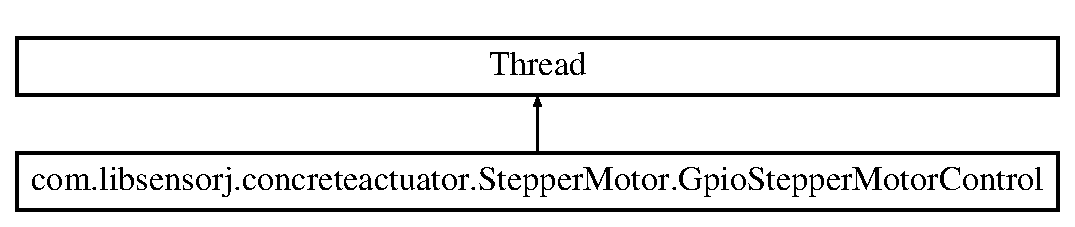
\includegraphics[height=2.000000cm]{classcom_1_1libsensorj_1_1concreteactuator_1_1StepperMotor_1_1GpioStepperMotorControl}
\end{center}
\end{figure}
\subsection*{Public Member Functions}
\begin{DoxyCompactItemize}
\item 
void \hyperlink{classcom_1_1libsensorj_1_1concreteactuator_1_1StepperMotor_1_1GpioStepperMotorControl_a04919aace52a0f604ecba747b231bbd0}{run} ()
\end{DoxyCompactItemize}


\subsection{Member Function Documentation}
\hypertarget{classcom_1_1libsensorj_1_1concreteactuator_1_1StepperMotor_1_1GpioStepperMotorControl_a04919aace52a0f604ecba747b231bbd0}{}\index{com\+::libsensorj\+::concreteactuator\+::\+Stepper\+Motor\+::\+Gpio\+Stepper\+Motor\+Control@{com\+::libsensorj\+::concreteactuator\+::\+Stepper\+Motor\+::\+Gpio\+Stepper\+Motor\+Control}!run@{run}}
\index{run@{run}!com\+::libsensorj\+::concreteactuator\+::\+Stepper\+Motor\+::\+Gpio\+Stepper\+Motor\+Control@{com\+::libsensorj\+::concreteactuator\+::\+Stepper\+Motor\+::\+Gpio\+Stepper\+Motor\+Control}}
\subsubsection[{run}]{\setlength{\rightskip}{0pt plus 5cm}void com.\+libsensorj.\+concreteactuator.\+Stepper\+Motor.\+Gpio\+Stepper\+Motor\+Control.\+run (
\begin{DoxyParamCaption}
{}
\end{DoxyParamCaption}
)}\label{classcom_1_1libsensorj_1_1concreteactuator_1_1StepperMotor_1_1GpioStepperMotorControl_a04919aace52a0f604ecba747b231bbd0}


The documentation for this class was generated from the following file\+:\begin{DoxyCompactItemize}
\item 
main/java/com/libsensorj/concreteactuator/\hyperlink{StepperMotor_8java}{Stepper\+Motor.\+java}\end{DoxyCompactItemize}

\hypertarget{classcom_1_1libsensorj_1_1concretesensor_1_1HCSR04Device}{}\section{com.\+libsensorj.\+concretesensor.\+H\+C\+S\+R04\+Device Class Reference}
\label{classcom_1_1libsensorj_1_1concretesensor_1_1HCSR04Device}\index{com.\+libsensorj.\+concretesensor.\+H\+C\+S\+R04\+Device@{com.\+libsensorj.\+concretesensor.\+H\+C\+S\+R04\+Device}}
Inheritance diagram for com.\+libsensorj.\+concretesensor.\+H\+C\+S\+R04\+Device\+:\begin{figure}[H]
\begin{center}
\leavevmode
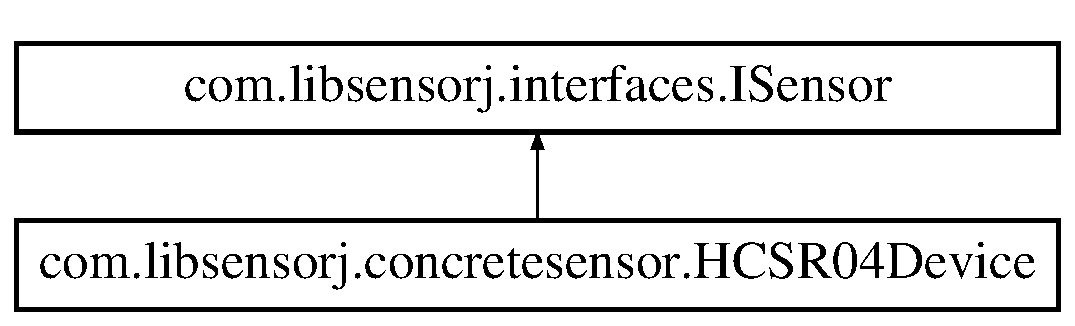
\includegraphics[height=2.000000cm]{classcom_1_1libsensorj_1_1concretesensor_1_1HCSR04Device}
\end{center}
\end{figure}
\subsection*{Public Member Functions}
\begin{DoxyCompactItemize}
\item 
\hyperlink{classcom_1_1libsensorj_1_1concretesensor_1_1HCSR04Device_ae0c7cdd02e374f360dff8d06a59b7c6d}{H\+C\+S\+R04\+Device} ()
\item 
\hyperlink{classcom_1_1libsensorj_1_1concretesensor_1_1HCSR04Device_a1c5c889b5ffe83c5fe8f7263bb8c8d33}{H\+C\+S\+R04\+Device} (int \+\_\+trigger, int \+\_\+echo)
\item 
\hyperlink{classcom_1_1libsensorj_1_1concretesensor_1_1HCSR04Device_a5148b245ef2aa510af815ecb3aeeb18b}{H\+C\+S\+R04\+Device} (Pin \+\_\+trigger, Pin \+\_\+echo)
\item 
void \hyperlink{classcom_1_1libsensorj_1_1concretesensor_1_1HCSR04Device_a3395de7d81b875516fb5c539accb27d1}{get\+Instance} ()
\item 
double \hyperlink{classcom_1_1libsensorj_1_1concretesensor_1_1HCSR04Device_aa30e4f6775819a36bc231a226c397bef}{get\+Distance} ()
\item 
void \hyperlink{classcom_1_1libsensorj_1_1concretesensor_1_1HCSR04Device_a69a3472b508507649ccb57e6fef81d6c}{close} ()
\end{DoxyCompactItemize}
\subsection*{Private Attributes}
\begin{DoxyCompactItemize}
\item 
Gpio\+Pin\+Digital\+Output \hyperlink{classcom_1_1libsensorj_1_1concretesensor_1_1HCSR04Device_ac898198f98143f7a1a4f281ea3c7c607}{trigger} = null
\item 
Gpio\+Pin\+Digital\+Input \hyperlink{classcom_1_1libsensorj_1_1concretesensor_1_1HCSR04Device_adf8ec00f094aefba690583e5a349c99d}{echo} = null
\end{DoxyCompactItemize}
\subsection*{Static Private Attributes}
\begin{DoxyCompactItemize}
\item 
static final int \hyperlink{classcom_1_1libsensorj_1_1concretesensor_1_1HCSR04Device_a1468a6c38c0086477a54eddbfe288299}{S\+P\+E\+E\+D\+O\+F\+S\+O\+U\+N\+D} = 34029
\item 
static final int \hyperlink{classcom_1_1libsensorj_1_1concretesensor_1_1HCSR04Device_a8f69accf3efa61a642b5e8693f7f158a}{T\+W\+O} = 2
\item 
static final long \hyperlink{classcom_1_1libsensorj_1_1concretesensor_1_1HCSR04Device_aaa527e39259b9e1be1b6360a397b3d30}{P\+U\+L\+S\+E\+\_\+\+T\+I\+M\+E} = 1
\item 
static final long \hyperlink{classcom_1_1libsensorj_1_1concretesensor_1_1HCSR04Device_a70071e4956bf93391031789b18039b6c}{D\+E\+L\+A\+Y} = 1000000000\+L
\item 
static final Logger \hyperlink{classcom_1_1libsensorj_1_1concretesensor_1_1HCSR04Device_a53449c0a7229928ddbb88c0d586cc63d}{L\+O\+G\+G\+E\+R}
\end{DoxyCompactItemize}


\subsection{Detailed Description}
The Class \hyperlink{classcom_1_1libsensorj_1_1concretesensor_1_1HCSR04Device}{H\+C\+S\+R04\+Device}. 

\subsection{Constructor \& Destructor Documentation}
\hypertarget{classcom_1_1libsensorj_1_1concretesensor_1_1HCSR04Device_ae0c7cdd02e374f360dff8d06a59b7c6d}{}\index{com\+::libsensorj\+::concretesensor\+::\+H\+C\+S\+R04\+Device@{com\+::libsensorj\+::concretesensor\+::\+H\+C\+S\+R04\+Device}!H\+C\+S\+R04\+Device@{H\+C\+S\+R04\+Device}}
\index{H\+C\+S\+R04\+Device@{H\+C\+S\+R04\+Device}!com\+::libsensorj\+::concretesensor\+::\+H\+C\+S\+R04\+Device@{com\+::libsensorj\+::concretesensor\+::\+H\+C\+S\+R04\+Device}}
\subsubsection[{H\+C\+S\+R04\+Device}]{\setlength{\rightskip}{0pt plus 5cm}com.\+libsensorj.\+concretesensor.\+H\+C\+S\+R04\+Device.\+H\+C\+S\+R04\+Device (
\begin{DoxyParamCaption}
{}
\end{DoxyParamCaption}
)}\label{classcom_1_1libsensorj_1_1concretesensor_1_1HCSR04Device_ae0c7cdd02e374f360dff8d06a59b7c6d}
Instantiates a new H\+C\+S r04 device. \hypertarget{classcom_1_1libsensorj_1_1concretesensor_1_1HCSR04Device_a1c5c889b5ffe83c5fe8f7263bb8c8d33}{}\index{com\+::libsensorj\+::concretesensor\+::\+H\+C\+S\+R04\+Device@{com\+::libsensorj\+::concretesensor\+::\+H\+C\+S\+R04\+Device}!H\+C\+S\+R04\+Device@{H\+C\+S\+R04\+Device}}
\index{H\+C\+S\+R04\+Device@{H\+C\+S\+R04\+Device}!com\+::libsensorj\+::concretesensor\+::\+H\+C\+S\+R04\+Device@{com\+::libsensorj\+::concretesensor\+::\+H\+C\+S\+R04\+Device}}
\subsubsection[{H\+C\+S\+R04\+Device}]{\setlength{\rightskip}{0pt plus 5cm}com.\+libsensorj.\+concretesensor.\+H\+C\+S\+R04\+Device.\+H\+C\+S\+R04\+Device (
\begin{DoxyParamCaption}
\item[{int}]{\+\_\+trigger, }
\item[{int}]{\+\_\+echo}
\end{DoxyParamCaption}
)}\label{classcom_1_1libsensorj_1_1concretesensor_1_1HCSR04Device_a1c5c889b5ffe83c5fe8f7263bb8c8d33}
Instantiates a new H\+C\+S r04 device.


\begin{DoxyParams}{Parameters}
{\em \+\_\+trigger} & the trigger \\
\hline
{\em \+\_\+echo} & the echo \\
\hline
\end{DoxyParams}
\hypertarget{classcom_1_1libsensorj_1_1concretesensor_1_1HCSR04Device_a5148b245ef2aa510af815ecb3aeeb18b}{}\index{com\+::libsensorj\+::concretesensor\+::\+H\+C\+S\+R04\+Device@{com\+::libsensorj\+::concretesensor\+::\+H\+C\+S\+R04\+Device}!H\+C\+S\+R04\+Device@{H\+C\+S\+R04\+Device}}
\index{H\+C\+S\+R04\+Device@{H\+C\+S\+R04\+Device}!com\+::libsensorj\+::concretesensor\+::\+H\+C\+S\+R04\+Device@{com\+::libsensorj\+::concretesensor\+::\+H\+C\+S\+R04\+Device}}
\subsubsection[{H\+C\+S\+R04\+Device}]{\setlength{\rightskip}{0pt plus 5cm}com.\+libsensorj.\+concretesensor.\+H\+C\+S\+R04\+Device.\+H\+C\+S\+R04\+Device (
\begin{DoxyParamCaption}
\item[{Pin}]{\+\_\+trigger, }
\item[{Pin}]{\+\_\+echo}
\end{DoxyParamCaption}
)}\label{classcom_1_1libsensorj_1_1concretesensor_1_1HCSR04Device_a5148b245ef2aa510af815ecb3aeeb18b}
Instantiates a new H\+C\+S r04 device.


\begin{DoxyParams}{Parameters}
{\em \+\_\+trigger} & the \+\_\+trigger \\
\hline
{\em \+\_\+echo} & the \+\_\+echo \\
\hline
\end{DoxyParams}


\subsection{Member Function Documentation}
\hypertarget{classcom_1_1libsensorj_1_1concretesensor_1_1HCSR04Device_a69a3472b508507649ccb57e6fef81d6c}{}\index{com\+::libsensorj\+::concretesensor\+::\+H\+C\+S\+R04\+Device@{com\+::libsensorj\+::concretesensor\+::\+H\+C\+S\+R04\+Device}!close@{close}}
\index{close@{close}!com\+::libsensorj\+::concretesensor\+::\+H\+C\+S\+R04\+Device@{com\+::libsensorj\+::concretesensor\+::\+H\+C\+S\+R04\+Device}}
\subsubsection[{close}]{\setlength{\rightskip}{0pt plus 5cm}void com.\+libsensorj.\+concretesensor.\+H\+C\+S\+R04\+Device.\+close (
\begin{DoxyParamCaption}
{}
\end{DoxyParamCaption}
)}\label{classcom_1_1libsensorj_1_1concretesensor_1_1HCSR04Device_a69a3472b508507649ccb57e6fef81d6c}
Close. \hypertarget{classcom_1_1libsensorj_1_1concretesensor_1_1HCSR04Device_aa30e4f6775819a36bc231a226c397bef}{}\index{com\+::libsensorj\+::concretesensor\+::\+H\+C\+S\+R04\+Device@{com\+::libsensorj\+::concretesensor\+::\+H\+C\+S\+R04\+Device}!get\+Distance@{get\+Distance}}
\index{get\+Distance@{get\+Distance}!com\+::libsensorj\+::concretesensor\+::\+H\+C\+S\+R04\+Device@{com\+::libsensorj\+::concretesensor\+::\+H\+C\+S\+R04\+Device}}
\subsubsection[{get\+Distance}]{\setlength{\rightskip}{0pt plus 5cm}double com.\+libsensorj.\+concretesensor.\+H\+C\+S\+R04\+Device.\+get\+Distance (
\begin{DoxyParamCaption}
{}
\end{DoxyParamCaption}
)}\label{classcom_1_1libsensorj_1_1concretesensor_1_1HCSR04Device_aa30e4f6775819a36bc231a226c397bef}
Gets the distance.

\begin{DoxyReturn}{Returns}
the distance 
\end{DoxyReturn}
\hypertarget{classcom_1_1libsensorj_1_1concretesensor_1_1HCSR04Device_a3395de7d81b875516fb5c539accb27d1}{}\index{com\+::libsensorj\+::concretesensor\+::\+H\+C\+S\+R04\+Device@{com\+::libsensorj\+::concretesensor\+::\+H\+C\+S\+R04\+Device}!get\+Instance@{get\+Instance}}
\index{get\+Instance@{get\+Instance}!com\+::libsensorj\+::concretesensor\+::\+H\+C\+S\+R04\+Device@{com\+::libsensorj\+::concretesensor\+::\+H\+C\+S\+R04\+Device}}
\subsubsection[{get\+Instance}]{\setlength{\rightskip}{0pt plus 5cm}void com.\+libsensorj.\+concretesensor.\+H\+C\+S\+R04\+Device.\+get\+Instance (
\begin{DoxyParamCaption}
{}
\end{DoxyParamCaption}
)}\label{classcom_1_1libsensorj_1_1concretesensor_1_1HCSR04Device_a3395de7d81b875516fb5c539accb27d1}
Gets the single instance of I\+Sensor.

\begin{DoxyReturn}{Returns}
single instance of I\+Sensor 
\end{DoxyReturn}


Implements \hyperlink{interfacecom_1_1libsensorj_1_1interfaces_1_1ISensor_a3c3db93a33adecde81a528651790f75e}{com.\+libsensorj.\+interfaces.\+I\+Sensor}.



\subsection{Member Data Documentation}
\hypertarget{classcom_1_1libsensorj_1_1concretesensor_1_1HCSR04Device_a70071e4956bf93391031789b18039b6c}{}\index{com\+::libsensorj\+::concretesensor\+::\+H\+C\+S\+R04\+Device@{com\+::libsensorj\+::concretesensor\+::\+H\+C\+S\+R04\+Device}!D\+E\+L\+A\+Y@{D\+E\+L\+A\+Y}}
\index{D\+E\+L\+A\+Y@{D\+E\+L\+A\+Y}!com\+::libsensorj\+::concretesensor\+::\+H\+C\+S\+R04\+Device@{com\+::libsensorj\+::concretesensor\+::\+H\+C\+S\+R04\+Device}}
\subsubsection[{D\+E\+L\+A\+Y}]{\setlength{\rightskip}{0pt plus 5cm}final long com.\+libsensorj.\+concretesensor.\+H\+C\+S\+R04\+Device.\+D\+E\+L\+A\+Y = 1000000000\+L\hspace{0.3cm}{\ttfamily [static]}, {\ttfamily [private]}}\label{classcom_1_1libsensorj_1_1concretesensor_1_1HCSR04Device_a70071e4956bf93391031789b18039b6c}
The Constant D\+E\+L\+A\+Y. \hypertarget{classcom_1_1libsensorj_1_1concretesensor_1_1HCSR04Device_adf8ec00f094aefba690583e5a349c99d}{}\index{com\+::libsensorj\+::concretesensor\+::\+H\+C\+S\+R04\+Device@{com\+::libsensorj\+::concretesensor\+::\+H\+C\+S\+R04\+Device}!echo@{echo}}
\index{echo@{echo}!com\+::libsensorj\+::concretesensor\+::\+H\+C\+S\+R04\+Device@{com\+::libsensorj\+::concretesensor\+::\+H\+C\+S\+R04\+Device}}
\subsubsection[{echo}]{\setlength{\rightskip}{0pt plus 5cm}Gpio\+Pin\+Digital\+Input com.\+libsensorj.\+concretesensor.\+H\+C\+S\+R04\+Device.\+echo = null\hspace{0.3cm}{\ttfamily [private]}}\label{classcom_1_1libsensorj_1_1concretesensor_1_1HCSR04Device_adf8ec00f094aefba690583e5a349c99d}
The echo. \hypertarget{classcom_1_1libsensorj_1_1concretesensor_1_1HCSR04Device_a53449c0a7229928ddbb88c0d586cc63d}{}\index{com\+::libsensorj\+::concretesensor\+::\+H\+C\+S\+R04\+Device@{com\+::libsensorj\+::concretesensor\+::\+H\+C\+S\+R04\+Device}!L\+O\+G\+G\+E\+R@{L\+O\+G\+G\+E\+R}}
\index{L\+O\+G\+G\+E\+R@{L\+O\+G\+G\+E\+R}!com\+::libsensorj\+::concretesensor\+::\+H\+C\+S\+R04\+Device@{com\+::libsensorj\+::concretesensor\+::\+H\+C\+S\+R04\+Device}}
\subsubsection[{L\+O\+G\+G\+E\+R}]{\setlength{\rightskip}{0pt plus 5cm}final Logger com.\+libsensorj.\+concretesensor.\+H\+C\+S\+R04\+Device.\+L\+O\+G\+G\+E\+R\hspace{0.3cm}{\ttfamily [static]}, {\ttfamily [private]}}\label{classcom_1_1libsensorj_1_1concretesensor_1_1HCSR04Device_a53449c0a7229928ddbb88c0d586cc63d}
{\bfseries Initial value\+:}
\begin{DoxyCode}
= LogManager
            .getLogger(\hyperlink{classcom_1_1libsensorj_1_1concretesensor_1_1HCSR04Device_ae0c7cdd02e374f360dff8d06a59b7c6d}{HCSR04Device}.class.getName())
\end{DoxyCode}
The Constant L\+O\+G\+G\+E\+R. \hypertarget{classcom_1_1libsensorj_1_1concretesensor_1_1HCSR04Device_aaa527e39259b9e1be1b6360a397b3d30}{}\index{com\+::libsensorj\+::concretesensor\+::\+H\+C\+S\+R04\+Device@{com\+::libsensorj\+::concretesensor\+::\+H\+C\+S\+R04\+Device}!P\+U\+L\+S\+E\+\_\+\+T\+I\+M\+E@{P\+U\+L\+S\+E\+\_\+\+T\+I\+M\+E}}
\index{P\+U\+L\+S\+E\+\_\+\+T\+I\+M\+E@{P\+U\+L\+S\+E\+\_\+\+T\+I\+M\+E}!com\+::libsensorj\+::concretesensor\+::\+H\+C\+S\+R04\+Device@{com\+::libsensorj\+::concretesensor\+::\+H\+C\+S\+R04\+Device}}
\subsubsection[{P\+U\+L\+S\+E\+\_\+\+T\+I\+M\+E}]{\setlength{\rightskip}{0pt plus 5cm}final long com.\+libsensorj.\+concretesensor.\+H\+C\+S\+R04\+Device.\+P\+U\+L\+S\+E\+\_\+\+T\+I\+M\+E = 1\hspace{0.3cm}{\ttfamily [static]}, {\ttfamily [private]}}\label{classcom_1_1libsensorj_1_1concretesensor_1_1HCSR04Device_aaa527e39259b9e1be1b6360a397b3d30}
The Constant P\+U\+L\+S\+E\+\_\+\+T\+I\+M\+E. \hypertarget{classcom_1_1libsensorj_1_1concretesensor_1_1HCSR04Device_a1468a6c38c0086477a54eddbfe288299}{}\index{com\+::libsensorj\+::concretesensor\+::\+H\+C\+S\+R04\+Device@{com\+::libsensorj\+::concretesensor\+::\+H\+C\+S\+R04\+Device}!S\+P\+E\+E\+D\+O\+F\+S\+O\+U\+N\+D@{S\+P\+E\+E\+D\+O\+F\+S\+O\+U\+N\+D}}
\index{S\+P\+E\+E\+D\+O\+F\+S\+O\+U\+N\+D@{S\+P\+E\+E\+D\+O\+F\+S\+O\+U\+N\+D}!com\+::libsensorj\+::concretesensor\+::\+H\+C\+S\+R04\+Device@{com\+::libsensorj\+::concretesensor\+::\+H\+C\+S\+R04\+Device}}
\subsubsection[{S\+P\+E\+E\+D\+O\+F\+S\+O\+U\+N\+D}]{\setlength{\rightskip}{0pt plus 5cm}final int com.\+libsensorj.\+concretesensor.\+H\+C\+S\+R04\+Device.\+S\+P\+E\+E\+D\+O\+F\+S\+O\+U\+N\+D = 34029\hspace{0.3cm}{\ttfamily [static]}, {\ttfamily [private]}}\label{classcom_1_1libsensorj_1_1concretesensor_1_1HCSR04Device_a1468a6c38c0086477a54eddbfe288299}
The Constant S\+P\+E\+E\+D\+O\+F\+S\+O\+U\+N\+D. \hypertarget{classcom_1_1libsensorj_1_1concretesensor_1_1HCSR04Device_ac898198f98143f7a1a4f281ea3c7c607}{}\index{com\+::libsensorj\+::concretesensor\+::\+H\+C\+S\+R04\+Device@{com\+::libsensorj\+::concretesensor\+::\+H\+C\+S\+R04\+Device}!trigger@{trigger}}
\index{trigger@{trigger}!com\+::libsensorj\+::concretesensor\+::\+H\+C\+S\+R04\+Device@{com\+::libsensorj\+::concretesensor\+::\+H\+C\+S\+R04\+Device}}
\subsubsection[{trigger}]{\setlength{\rightskip}{0pt plus 5cm}Gpio\+Pin\+Digital\+Output com.\+libsensorj.\+concretesensor.\+H\+C\+S\+R04\+Device.\+trigger = null\hspace{0.3cm}{\ttfamily [private]}}\label{classcom_1_1libsensorj_1_1concretesensor_1_1HCSR04Device_ac898198f98143f7a1a4f281ea3c7c607}
The trigger. \hypertarget{classcom_1_1libsensorj_1_1concretesensor_1_1HCSR04Device_a8f69accf3efa61a642b5e8693f7f158a}{}\index{com\+::libsensorj\+::concretesensor\+::\+H\+C\+S\+R04\+Device@{com\+::libsensorj\+::concretesensor\+::\+H\+C\+S\+R04\+Device}!T\+W\+O@{T\+W\+O}}
\index{T\+W\+O@{T\+W\+O}!com\+::libsensorj\+::concretesensor\+::\+H\+C\+S\+R04\+Device@{com\+::libsensorj\+::concretesensor\+::\+H\+C\+S\+R04\+Device}}
\subsubsection[{T\+W\+O}]{\setlength{\rightskip}{0pt plus 5cm}final int com.\+libsensorj.\+concretesensor.\+H\+C\+S\+R04\+Device.\+T\+W\+O = 2\hspace{0.3cm}{\ttfamily [static]}, {\ttfamily [private]}}\label{classcom_1_1libsensorj_1_1concretesensor_1_1HCSR04Device_a8f69accf3efa61a642b5e8693f7f158a}
The Constant T\+W\+O. 

The documentation for this class was generated from the following file\+:\begin{DoxyCompactItemize}
\item 
main/java/com/libsensorj/concretesensor/\hyperlink{HCSR04Device_8java}{H\+C\+S\+R04\+Device.\+java}\end{DoxyCompactItemize}

\hypertarget{classcom_1_1libsensorj_1_1examples_1_1HCSR04DeviceExample}{}\section{com.\+libsensorj.\+examples.\+H\+C\+S\+R04\+Device\+Example Class Reference}
\label{classcom_1_1libsensorj_1_1examples_1_1HCSR04DeviceExample}\index{com.\+libsensorj.\+examples.\+H\+C\+S\+R04\+Device\+Example@{com.\+libsensorj.\+examples.\+H\+C\+S\+R04\+Device\+Example}}
\subsection*{Static Public Member Functions}
\begin{DoxyCompactItemize}
\item 
static void \hyperlink{classcom_1_1libsensorj_1_1examples_1_1HCSR04DeviceExample_ab213367036bb78e1b6614967207a718a}{main} (String\mbox{[}$\,$\mbox{]} args)
\end{DoxyCompactItemize}
\subsection*{Static Private Attributes}
\begin{DoxyCompactItemize}
\item 
static \hyperlink{interfacecom_1_1libsensorj_1_1interfaces_1_1ISensor}{I\+Sensor} \hyperlink{classcom_1_1libsensorj_1_1examples_1_1HCSR04DeviceExample_aa4f457230d5989c781e4c142492cf9c2}{hcsr}
\item 
static final Logger \hyperlink{classcom_1_1libsensorj_1_1examples_1_1HCSR04DeviceExample_a156f69717cfae755de776e6310ae212f}{L\+O\+G\+G\+E\+R}
\end{DoxyCompactItemize}


\subsection{Detailed Description}
The Class \hyperlink{classcom_1_1libsensorj_1_1examples_1_1HCSR04DeviceExample}{H\+C\+S\+R04\+Device\+Example}. 

\subsection{Member Function Documentation}
\hypertarget{classcom_1_1libsensorj_1_1examples_1_1HCSR04DeviceExample_ab213367036bb78e1b6614967207a718a}{}\index{com\+::libsensorj\+::examples\+::\+H\+C\+S\+R04\+Device\+Example@{com\+::libsensorj\+::examples\+::\+H\+C\+S\+R04\+Device\+Example}!main@{main}}
\index{main@{main}!com\+::libsensorj\+::examples\+::\+H\+C\+S\+R04\+Device\+Example@{com\+::libsensorj\+::examples\+::\+H\+C\+S\+R04\+Device\+Example}}
\subsubsection[{main}]{\setlength{\rightskip}{0pt plus 5cm}static void com.\+libsensorj.\+examples.\+H\+C\+S\+R04\+Device\+Example.\+main (
\begin{DoxyParamCaption}
\item[{String\mbox{[}$\,$\mbox{]}}]{args}
\end{DoxyParamCaption}
)\hspace{0.3cm}{\ttfamily [static]}}\label{classcom_1_1libsensorj_1_1examples_1_1HCSR04DeviceExample_ab213367036bb78e1b6614967207a718a}
The main method.


\begin{DoxyParams}{Parameters}
{\em args} & the arguments \\
\hline
\end{DoxyParams}


\subsection{Member Data Documentation}
\hypertarget{classcom_1_1libsensorj_1_1examples_1_1HCSR04DeviceExample_aa4f457230d5989c781e4c142492cf9c2}{}\index{com\+::libsensorj\+::examples\+::\+H\+C\+S\+R04\+Device\+Example@{com\+::libsensorj\+::examples\+::\+H\+C\+S\+R04\+Device\+Example}!hcsr@{hcsr}}
\index{hcsr@{hcsr}!com\+::libsensorj\+::examples\+::\+H\+C\+S\+R04\+Device\+Example@{com\+::libsensorj\+::examples\+::\+H\+C\+S\+R04\+Device\+Example}}
\subsubsection[{hcsr}]{\setlength{\rightskip}{0pt plus 5cm}{\bf I\+Sensor} com.\+libsensorj.\+examples.\+H\+C\+S\+R04\+Device\+Example.\+hcsr\hspace{0.3cm}{\ttfamily [static]}, {\ttfamily [private]}}\label{classcom_1_1libsensorj_1_1examples_1_1HCSR04DeviceExample_aa4f457230d5989c781e4c142492cf9c2}
The I\+Sensor hcsr. \hypertarget{classcom_1_1libsensorj_1_1examples_1_1HCSR04DeviceExample_a156f69717cfae755de776e6310ae212f}{}\index{com\+::libsensorj\+::examples\+::\+H\+C\+S\+R04\+Device\+Example@{com\+::libsensorj\+::examples\+::\+H\+C\+S\+R04\+Device\+Example}!L\+O\+G\+G\+E\+R@{L\+O\+G\+G\+E\+R}}
\index{L\+O\+G\+G\+E\+R@{L\+O\+G\+G\+E\+R}!com\+::libsensorj\+::examples\+::\+H\+C\+S\+R04\+Device\+Example@{com\+::libsensorj\+::examples\+::\+H\+C\+S\+R04\+Device\+Example}}
\subsubsection[{L\+O\+G\+G\+E\+R}]{\setlength{\rightskip}{0pt plus 5cm}final Logger com.\+libsensorj.\+examples.\+H\+C\+S\+R04\+Device\+Example.\+L\+O\+G\+G\+E\+R\hspace{0.3cm}{\ttfamily [static]}, {\ttfamily [private]}}\label{classcom_1_1libsensorj_1_1examples_1_1HCSR04DeviceExample_a156f69717cfae755de776e6310ae212f}
{\bfseries Initial value\+:}
\begin{DoxyCode}
= LogManager
            .getLogger(HCSR04DeviceExample.class.getName())
\end{DoxyCode}
The Constant L\+O\+G\+G\+E\+R. 

The documentation for this class was generated from the following file\+:\begin{DoxyCompactItemize}
\item 
main/java/com/libsensorj/examples/\hyperlink{HCSR04DeviceExample_8java}{H\+C\+S\+R04\+Device\+Example.\+java}\end{DoxyCompactItemize}

\hypertarget{classcom_1_1libsensorj_1_1concretefactory_1_1HCSR04DeviceFactory}{}\section{com.\+libsensorj.\+concretefactory.\+H\+C\+S\+R04\+Device\+Factory Class Reference}
\label{classcom_1_1libsensorj_1_1concretefactory_1_1HCSR04DeviceFactory}\index{com.\+libsensorj.\+concretefactory.\+H\+C\+S\+R04\+Device\+Factory@{com.\+libsensorj.\+concretefactory.\+H\+C\+S\+R04\+Device\+Factory}}
Inheritance diagram for com.\+libsensorj.\+concretefactory.\+H\+C\+S\+R04\+Device\+Factory\+:\begin{figure}[H]
\begin{center}
\leavevmode
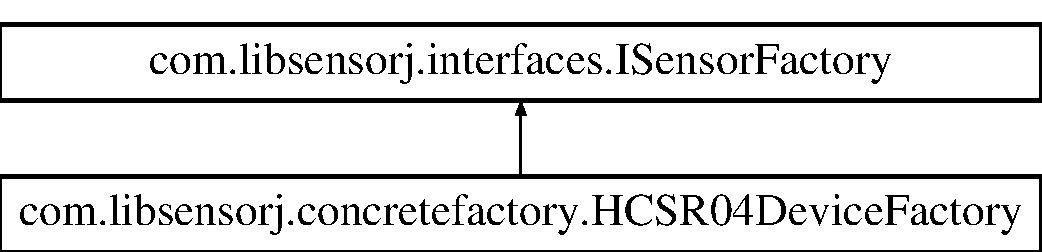
\includegraphics[height=2.000000cm]{classcom_1_1libsensorj_1_1concretefactory_1_1HCSR04DeviceFactory}
\end{center}
\end{figure}
\subsection*{Public Member Functions}
\begin{DoxyCompactItemize}
\item 
\hyperlink{interfacecom_1_1libsensorj_1_1interfaces_1_1ISensor}{I\+Sensor} \hyperlink{classcom_1_1libsensorj_1_1concretefactory_1_1HCSR04DeviceFactory_a3d5c07b9ce458a3f56cfe5e7470b51df}{create\+Sensor} ()
\item 
\hyperlink{classcom_1_1libsensorj_1_1interfaces_1_1IEvent}{I\+Event} \hyperlink{classcom_1_1libsensorj_1_1concretefactory_1_1HCSR04DeviceFactory_aea88b0202d3021c4e55bd9cbf64da906}{create\+Event} ()
\end{DoxyCompactItemize}


\subsection{Detailed Description}
A factory for creating H\+C\+S\+R04\+Device objects. 

\subsection{Member Function Documentation}
\hypertarget{classcom_1_1libsensorj_1_1concretefactory_1_1HCSR04DeviceFactory_aea88b0202d3021c4e55bd9cbf64da906}{}\index{com\+::libsensorj\+::concretefactory\+::\+H\+C\+S\+R04\+Device\+Factory@{com\+::libsensorj\+::concretefactory\+::\+H\+C\+S\+R04\+Device\+Factory}!create\+Event@{create\+Event}}
\index{create\+Event@{create\+Event}!com\+::libsensorj\+::concretefactory\+::\+H\+C\+S\+R04\+Device\+Factory@{com\+::libsensorj\+::concretefactory\+::\+H\+C\+S\+R04\+Device\+Factory}}
\subsubsection[{create\+Event}]{\setlength{\rightskip}{0pt plus 5cm}{\bf I\+Event} com.\+libsensorj.\+concretefactory.\+H\+C\+S\+R04\+Device\+Factory.\+create\+Event (
\begin{DoxyParamCaption}
{}
\end{DoxyParamCaption}
)}\label{classcom_1_1libsensorj_1_1concretefactory_1_1HCSR04DeviceFactory_aea88b0202d3021c4e55bd9cbf64da906}
Creates a new I\+Event object.

\begin{DoxyReturn}{Returns}
the I\+Event 
\end{DoxyReturn}


Implements \hyperlink{interfacecom_1_1libsensorj_1_1interfaces_1_1ISensorFactory_a2b074d01287a4e64677097255ba9e768}{com.\+libsensorj.\+interfaces.\+I\+Sensor\+Factory}.

\hypertarget{classcom_1_1libsensorj_1_1concretefactory_1_1HCSR04DeviceFactory_a3d5c07b9ce458a3f56cfe5e7470b51df}{}\index{com\+::libsensorj\+::concretefactory\+::\+H\+C\+S\+R04\+Device\+Factory@{com\+::libsensorj\+::concretefactory\+::\+H\+C\+S\+R04\+Device\+Factory}!create\+Sensor@{create\+Sensor}}
\index{create\+Sensor@{create\+Sensor}!com\+::libsensorj\+::concretefactory\+::\+H\+C\+S\+R04\+Device\+Factory@{com\+::libsensorj\+::concretefactory\+::\+H\+C\+S\+R04\+Device\+Factory}}
\subsubsection[{create\+Sensor}]{\setlength{\rightskip}{0pt plus 5cm}{\bf I\+Sensor} com.\+libsensorj.\+concretefactory.\+H\+C\+S\+R04\+Device\+Factory.\+create\+Sensor (
\begin{DoxyParamCaption}
{}
\end{DoxyParamCaption}
)}\label{classcom_1_1libsensorj_1_1concretefactory_1_1HCSR04DeviceFactory_a3d5c07b9ce458a3f56cfe5e7470b51df}
Creates a new I\+Sensor object.

\begin{DoxyReturn}{Returns}
the I\+Sensor 
\end{DoxyReturn}


Implements \hyperlink{interfacecom_1_1libsensorj_1_1interfaces_1_1ISensorFactory_ac14c6d566c37c6a79c6db1e85634f25d}{com.\+libsensorj.\+interfaces.\+I\+Sensor\+Factory}.



The documentation for this class was generated from the following file\+:\begin{DoxyCompactItemize}
\item 
main/java/com/libsensorj/concretefactory/\hyperlink{HCSR04DeviceFactory_8java}{H\+C\+S\+R04\+Device\+Factory.\+java}\end{DoxyCompactItemize}

\hypertarget{classcom_1_1libsensorj_1_1concretesensor_1_1test_1_1HCSR04DeviceTests}{}\section{com.\+libsensorj.\+concretesensor.\+test.\+H\+C\+S\+R04\+Device\+Tests Class Reference}
\label{classcom_1_1libsensorj_1_1concretesensor_1_1test_1_1HCSR04DeviceTests}\index{com.\+libsensorj.\+concretesensor.\+test.\+H\+C\+S\+R04\+Device\+Tests@{com.\+libsensorj.\+concretesensor.\+test.\+H\+C\+S\+R04\+Device\+Tests}}
\subsection*{Public Member Functions}
\begin{DoxyCompactItemize}
\item 
void \hyperlink{classcom_1_1libsensorj_1_1concretesensor_1_1test_1_1HCSR04DeviceTests_aa4827ef25ecda9d8fafae51e1a26f44a}{test\+Pin\+Provisioned} ()
\item 
void \hyperlink{classcom_1_1libsensorj_1_1concretesensor_1_1test_1_1HCSR04DeviceTests_a8d5faee8a1e20b225c1f410e2bb51155}{test\+Get\+Distance} ()
\end{DoxyCompactItemize}
\subsection*{Static Public Member Functions}
\begin{DoxyCompactItemize}
\item 
static void \hyperlink{classcom_1_1libsensorj_1_1concretesensor_1_1test_1_1HCSR04DeviceTests_a03c2c422c08b49925990bc542e72020a}{setup} ()
\end{DoxyCompactItemize}
\subsection*{Static Private Attributes}
\begin{DoxyCompactItemize}
\item 
static Gpio\+Controller \hyperlink{classcom_1_1libsensorj_1_1concretesensor_1_1test_1_1HCSR04DeviceTests_a633636296bc508c587ec96215ae90f49}{gpio}
\item 
static Gpio\+Pin\+Digital\+Output \hyperlink{classcom_1_1libsensorj_1_1concretesensor_1_1test_1_1HCSR04DeviceTests_a1284eaac23d3414b8115c58e3daf10c0}{trigger}
\item 
static Gpio\+Pin\+Digital\+Input \hyperlink{classcom_1_1libsensorj_1_1concretesensor_1_1test_1_1HCSR04DeviceTests_aa5c0c872aec976b3c6eba9ca14eaee21}{echo}
\item 
static Pin\+State \hyperlink{classcom_1_1libsensorj_1_1concretesensor_1_1test_1_1HCSR04DeviceTests_aa1dee7612489b95ae1e84834018f612c}{echo\+Monitored\+State}
\item 
static Pin\+State \hyperlink{classcom_1_1libsensorj_1_1concretesensor_1_1test_1_1HCSR04DeviceTests_ae6c52d9bfe127814bf0b2566d4671ef3}{trigger\+Monitored\+State}
\item 
static final String \hyperlink{classcom_1_1libsensorj_1_1concretesensor_1_1test_1_1HCSR04DeviceTests_a76e128e04a46245fcef0b87f377b9b7c}{D\+A\+T\+A\+\_\+\+R\+E\+A\+D\+E\+D} = \char`\"{}10\char`\"{}
\item 
static final String \hyperlink{classcom_1_1libsensorj_1_1concretesensor_1_1test_1_1HCSR04DeviceTests_a47cef441c2f68e1f55e5dfb6b1fef3c8}{D\+I\+S\+T\+A\+N\+C\+E\+\_\+\+M\+E\+T\+H\+O\+D} = \char`\"{}get\+Distance\char`\"{}
\item 
static final Logger \hyperlink{classcom_1_1libsensorj_1_1concretesensor_1_1test_1_1HCSR04DeviceTests_a5bceb1147cb539bde62dad0d4f95e3cf}{L\+O\+G\+G\+E\+R}
\end{DoxyCompactItemize}


\subsection{Member Function Documentation}
\hypertarget{classcom_1_1libsensorj_1_1concretesensor_1_1test_1_1HCSR04DeviceTests_a03c2c422c08b49925990bc542e72020a}{}\index{com\+::libsensorj\+::concretesensor\+::test\+::\+H\+C\+S\+R04\+Device\+Tests@{com\+::libsensorj\+::concretesensor\+::test\+::\+H\+C\+S\+R04\+Device\+Tests}!setup@{setup}}
\index{setup@{setup}!com\+::libsensorj\+::concretesensor\+::test\+::\+H\+C\+S\+R04\+Device\+Tests@{com\+::libsensorj\+::concretesensor\+::test\+::\+H\+C\+S\+R04\+Device\+Tests}}
\subsubsection[{setup}]{\setlength{\rightskip}{0pt plus 5cm}static void com.\+libsensorj.\+concretesensor.\+test.\+H\+C\+S\+R04\+Device\+Tests.\+setup (
\begin{DoxyParamCaption}
{}
\end{DoxyParamCaption}
)\hspace{0.3cm}{\ttfamily [static]}}\label{classcom_1_1libsensorj_1_1concretesensor_1_1test_1_1HCSR04DeviceTests_a03c2c422c08b49925990bc542e72020a}
Setup. \hypertarget{classcom_1_1libsensorj_1_1concretesensor_1_1test_1_1HCSR04DeviceTests_a8d5faee8a1e20b225c1f410e2bb51155}{}\index{com\+::libsensorj\+::concretesensor\+::test\+::\+H\+C\+S\+R04\+Device\+Tests@{com\+::libsensorj\+::concretesensor\+::test\+::\+H\+C\+S\+R04\+Device\+Tests}!test\+Get\+Distance@{test\+Get\+Distance}}
\index{test\+Get\+Distance@{test\+Get\+Distance}!com\+::libsensorj\+::concretesensor\+::test\+::\+H\+C\+S\+R04\+Device\+Tests@{com\+::libsensorj\+::concretesensor\+::test\+::\+H\+C\+S\+R04\+Device\+Tests}}
\subsubsection[{test\+Get\+Distance}]{\setlength{\rightskip}{0pt plus 5cm}void com.\+libsensorj.\+concretesensor.\+test.\+H\+C\+S\+R04\+Device\+Tests.\+test\+Get\+Distance (
\begin{DoxyParamCaption}
{}
\end{DoxyParamCaption}
)}\label{classcom_1_1libsensorj_1_1concretesensor_1_1test_1_1HCSR04DeviceTests_a8d5faee8a1e20b225c1f410e2bb51155}
Test Get\+Humidity. \hypertarget{classcom_1_1libsensorj_1_1concretesensor_1_1test_1_1HCSR04DeviceTests_aa4827ef25ecda9d8fafae51e1a26f44a}{}\index{com\+::libsensorj\+::concretesensor\+::test\+::\+H\+C\+S\+R04\+Device\+Tests@{com\+::libsensorj\+::concretesensor\+::test\+::\+H\+C\+S\+R04\+Device\+Tests}!test\+Pin\+Provisioned@{test\+Pin\+Provisioned}}
\index{test\+Pin\+Provisioned@{test\+Pin\+Provisioned}!com\+::libsensorj\+::concretesensor\+::test\+::\+H\+C\+S\+R04\+Device\+Tests@{com\+::libsensorj\+::concretesensor\+::test\+::\+H\+C\+S\+R04\+Device\+Tests}}
\subsubsection[{test\+Pin\+Provisioned}]{\setlength{\rightskip}{0pt plus 5cm}void com.\+libsensorj.\+concretesensor.\+test.\+H\+C\+S\+R04\+Device\+Tests.\+test\+Pin\+Provisioned (
\begin{DoxyParamCaption}
{}
\end{DoxyParamCaption}
)}\label{classcom_1_1libsensorj_1_1concretesensor_1_1test_1_1HCSR04DeviceTests_aa4827ef25ecda9d8fafae51e1a26f44a}
Test pin provisioned. 

\subsection{Member Data Documentation}
\hypertarget{classcom_1_1libsensorj_1_1concretesensor_1_1test_1_1HCSR04DeviceTests_a76e128e04a46245fcef0b87f377b9b7c}{}\index{com\+::libsensorj\+::concretesensor\+::test\+::\+H\+C\+S\+R04\+Device\+Tests@{com\+::libsensorj\+::concretesensor\+::test\+::\+H\+C\+S\+R04\+Device\+Tests}!D\+A\+T\+A\+\_\+\+R\+E\+A\+D\+E\+D@{D\+A\+T\+A\+\_\+\+R\+E\+A\+D\+E\+D}}
\index{D\+A\+T\+A\+\_\+\+R\+E\+A\+D\+E\+D@{D\+A\+T\+A\+\_\+\+R\+E\+A\+D\+E\+D}!com\+::libsensorj\+::concretesensor\+::test\+::\+H\+C\+S\+R04\+Device\+Tests@{com\+::libsensorj\+::concretesensor\+::test\+::\+H\+C\+S\+R04\+Device\+Tests}}
\subsubsection[{D\+A\+T\+A\+\_\+\+R\+E\+A\+D\+E\+D}]{\setlength{\rightskip}{0pt plus 5cm}final String com.\+libsensorj.\+concretesensor.\+test.\+H\+C\+S\+R04\+Device\+Tests.\+D\+A\+T\+A\+\_\+\+R\+E\+A\+D\+E\+D = \char`\"{}10\char`\"{}\hspace{0.3cm}{\ttfamily [static]}, {\ttfamily [private]}}\label{classcom_1_1libsensorj_1_1concretesensor_1_1test_1_1HCSR04DeviceTests_a76e128e04a46245fcef0b87f377b9b7c}
The Constant D\+A\+T\+A\+\_\+\+R\+E\+A\+D\+E\+D. \hypertarget{classcom_1_1libsensorj_1_1concretesensor_1_1test_1_1HCSR04DeviceTests_a47cef441c2f68e1f55e5dfb6b1fef3c8}{}\index{com\+::libsensorj\+::concretesensor\+::test\+::\+H\+C\+S\+R04\+Device\+Tests@{com\+::libsensorj\+::concretesensor\+::test\+::\+H\+C\+S\+R04\+Device\+Tests}!D\+I\+S\+T\+A\+N\+C\+E\+\_\+\+M\+E\+T\+H\+O\+D@{D\+I\+S\+T\+A\+N\+C\+E\+\_\+\+M\+E\+T\+H\+O\+D}}
\index{D\+I\+S\+T\+A\+N\+C\+E\+\_\+\+M\+E\+T\+H\+O\+D@{D\+I\+S\+T\+A\+N\+C\+E\+\_\+\+M\+E\+T\+H\+O\+D}!com\+::libsensorj\+::concretesensor\+::test\+::\+H\+C\+S\+R04\+Device\+Tests@{com\+::libsensorj\+::concretesensor\+::test\+::\+H\+C\+S\+R04\+Device\+Tests}}
\subsubsection[{D\+I\+S\+T\+A\+N\+C\+E\+\_\+\+M\+E\+T\+H\+O\+D}]{\setlength{\rightskip}{0pt plus 5cm}final String com.\+libsensorj.\+concretesensor.\+test.\+H\+C\+S\+R04\+Device\+Tests.\+D\+I\+S\+T\+A\+N\+C\+E\+\_\+\+M\+E\+T\+H\+O\+D = \char`\"{}get\+Distance\char`\"{}\hspace{0.3cm}{\ttfamily [static]}, {\ttfamily [private]}}\label{classcom_1_1libsensorj_1_1concretesensor_1_1test_1_1HCSR04DeviceTests_a47cef441c2f68e1f55e5dfb6b1fef3c8}
The Constant R\+E\+A\+D\+V\+A\+L\+U\+E\+S\+\_\+\+M\+E\+T\+H\+O\+D. \hypertarget{classcom_1_1libsensorj_1_1concretesensor_1_1test_1_1HCSR04DeviceTests_aa5c0c872aec976b3c6eba9ca14eaee21}{}\index{com\+::libsensorj\+::concretesensor\+::test\+::\+H\+C\+S\+R04\+Device\+Tests@{com\+::libsensorj\+::concretesensor\+::test\+::\+H\+C\+S\+R04\+Device\+Tests}!echo@{echo}}
\index{echo@{echo}!com\+::libsensorj\+::concretesensor\+::test\+::\+H\+C\+S\+R04\+Device\+Tests@{com\+::libsensorj\+::concretesensor\+::test\+::\+H\+C\+S\+R04\+Device\+Tests}}
\subsubsection[{echo}]{\setlength{\rightskip}{0pt plus 5cm}Gpio\+Pin\+Digital\+Input com.\+libsensorj.\+concretesensor.\+test.\+H\+C\+S\+R04\+Device\+Tests.\+echo\hspace{0.3cm}{\ttfamily [static]}, {\ttfamily [private]}}\label{classcom_1_1libsensorj_1_1concretesensor_1_1test_1_1HCSR04DeviceTests_aa5c0c872aec976b3c6eba9ca14eaee21}
The pin. \hypertarget{classcom_1_1libsensorj_1_1concretesensor_1_1test_1_1HCSR04DeviceTests_aa1dee7612489b95ae1e84834018f612c}{}\index{com\+::libsensorj\+::concretesensor\+::test\+::\+H\+C\+S\+R04\+Device\+Tests@{com\+::libsensorj\+::concretesensor\+::test\+::\+H\+C\+S\+R04\+Device\+Tests}!echo\+Monitored\+State@{echo\+Monitored\+State}}
\index{echo\+Monitored\+State@{echo\+Monitored\+State}!com\+::libsensorj\+::concretesensor\+::test\+::\+H\+C\+S\+R04\+Device\+Tests@{com\+::libsensorj\+::concretesensor\+::test\+::\+H\+C\+S\+R04\+Device\+Tests}}
\subsubsection[{echo\+Monitored\+State}]{\setlength{\rightskip}{0pt plus 5cm}Pin\+State com.\+libsensorj.\+concretesensor.\+test.\+H\+C\+S\+R04\+Device\+Tests.\+echo\+Monitored\+State\hspace{0.3cm}{\ttfamily [static]}, {\ttfamily [private]}}\label{classcom_1_1libsensorj_1_1concretesensor_1_1test_1_1HCSR04DeviceTests_aa1dee7612489b95ae1e84834018f612c}
The pin monitored state. \hypertarget{classcom_1_1libsensorj_1_1concretesensor_1_1test_1_1HCSR04DeviceTests_a633636296bc508c587ec96215ae90f49}{}\index{com\+::libsensorj\+::concretesensor\+::test\+::\+H\+C\+S\+R04\+Device\+Tests@{com\+::libsensorj\+::concretesensor\+::test\+::\+H\+C\+S\+R04\+Device\+Tests}!gpio@{gpio}}
\index{gpio@{gpio}!com\+::libsensorj\+::concretesensor\+::test\+::\+H\+C\+S\+R04\+Device\+Tests@{com\+::libsensorj\+::concretesensor\+::test\+::\+H\+C\+S\+R04\+Device\+Tests}}
\subsubsection[{gpio}]{\setlength{\rightskip}{0pt plus 5cm}Gpio\+Controller com.\+libsensorj.\+concretesensor.\+test.\+H\+C\+S\+R04\+Device\+Tests.\+gpio\hspace{0.3cm}{\ttfamily [static]}, {\ttfamily [private]}}\label{classcom_1_1libsensorj_1_1concretesensor_1_1test_1_1HCSR04DeviceTests_a633636296bc508c587ec96215ae90f49}
The provider. The gpio. \hypertarget{classcom_1_1libsensorj_1_1concretesensor_1_1test_1_1HCSR04DeviceTests_a5bceb1147cb539bde62dad0d4f95e3cf}{}\index{com\+::libsensorj\+::concretesensor\+::test\+::\+H\+C\+S\+R04\+Device\+Tests@{com\+::libsensorj\+::concretesensor\+::test\+::\+H\+C\+S\+R04\+Device\+Tests}!L\+O\+G\+G\+E\+R@{L\+O\+G\+G\+E\+R}}
\index{L\+O\+G\+G\+E\+R@{L\+O\+G\+G\+E\+R}!com\+::libsensorj\+::concretesensor\+::test\+::\+H\+C\+S\+R04\+Device\+Tests@{com\+::libsensorj\+::concretesensor\+::test\+::\+H\+C\+S\+R04\+Device\+Tests}}
\subsubsection[{L\+O\+G\+G\+E\+R}]{\setlength{\rightskip}{0pt plus 5cm}final Logger com.\+libsensorj.\+concretesensor.\+test.\+H\+C\+S\+R04\+Device\+Tests.\+L\+O\+G\+G\+E\+R\hspace{0.3cm}{\ttfamily [static]}, {\ttfamily [private]}}\label{classcom_1_1libsensorj_1_1concretesensor_1_1test_1_1HCSR04DeviceTests_a5bceb1147cb539bde62dad0d4f95e3cf}
{\bfseries Initial value\+:}
\begin{DoxyCode}
= LogManager
            .getLogger(HCSR04DeviceTests.class.getName())
\end{DoxyCode}
The Constant L\+O\+G\+G\+E\+R. \hypertarget{classcom_1_1libsensorj_1_1concretesensor_1_1test_1_1HCSR04DeviceTests_a1284eaac23d3414b8115c58e3daf10c0}{}\index{com\+::libsensorj\+::concretesensor\+::test\+::\+H\+C\+S\+R04\+Device\+Tests@{com\+::libsensorj\+::concretesensor\+::test\+::\+H\+C\+S\+R04\+Device\+Tests}!trigger@{trigger}}
\index{trigger@{trigger}!com\+::libsensorj\+::concretesensor\+::test\+::\+H\+C\+S\+R04\+Device\+Tests@{com\+::libsensorj\+::concretesensor\+::test\+::\+H\+C\+S\+R04\+Device\+Tests}}
\subsubsection[{trigger}]{\setlength{\rightskip}{0pt plus 5cm}Gpio\+Pin\+Digital\+Output com.\+libsensorj.\+concretesensor.\+test.\+H\+C\+S\+R04\+Device\+Tests.\+trigger\hspace{0.3cm}{\ttfamily [static]}, {\ttfamily [private]}}\label{classcom_1_1libsensorj_1_1concretesensor_1_1test_1_1HCSR04DeviceTests_a1284eaac23d3414b8115c58e3daf10c0}
The pin. \hypertarget{classcom_1_1libsensorj_1_1concretesensor_1_1test_1_1HCSR04DeviceTests_ae6c52d9bfe127814bf0b2566d4671ef3}{}\index{com\+::libsensorj\+::concretesensor\+::test\+::\+H\+C\+S\+R04\+Device\+Tests@{com\+::libsensorj\+::concretesensor\+::test\+::\+H\+C\+S\+R04\+Device\+Tests}!trigger\+Monitored\+State@{trigger\+Monitored\+State}}
\index{trigger\+Monitored\+State@{trigger\+Monitored\+State}!com\+::libsensorj\+::concretesensor\+::test\+::\+H\+C\+S\+R04\+Device\+Tests@{com\+::libsensorj\+::concretesensor\+::test\+::\+H\+C\+S\+R04\+Device\+Tests}}
\subsubsection[{trigger\+Monitored\+State}]{\setlength{\rightskip}{0pt plus 5cm}Pin\+State com.\+libsensorj.\+concretesensor.\+test.\+H\+C\+S\+R04\+Device\+Tests.\+trigger\+Monitored\+State\hspace{0.3cm}{\ttfamily [static]}, {\ttfamily [private]}}\label{classcom_1_1libsensorj_1_1concretesensor_1_1test_1_1HCSR04DeviceTests_ae6c52d9bfe127814bf0b2566d4671ef3}
The pin monitored state. 

The documentation for this class was generated from the following file\+:\begin{DoxyCompactItemize}
\item 
test/java/com/libsensorj/concretesensor/test/\hyperlink{HCSR04DeviceTests_8java}{H\+C\+S\+R04\+Device\+Tests.\+java}\end{DoxyCompactItemize}

\hypertarget{classcom_1_1libsensorj_1_1examples_1_1HCSR04NoSensorClass}{}\section{com.\+libsensorj.\+examples.\+H\+C\+S\+R04\+No\+Sensor\+Class Class Reference}
\label{classcom_1_1libsensorj_1_1examples_1_1HCSR04NoSensorClass}\index{com.\+libsensorj.\+examples.\+H\+C\+S\+R04\+No\+Sensor\+Class@{com.\+libsensorj.\+examples.\+H\+C\+S\+R04\+No\+Sensor\+Class}}
\subsection*{Static Public Member Functions}
\begin{DoxyCompactItemize}
\item 
static void \hyperlink{classcom_1_1libsensorj_1_1examples_1_1HCSR04NoSensorClass_abbbd349b6d62a9488da92b355a3f01ff}{main} (String\mbox{[}$\,$\mbox{]} args)  throws Interrupted\+Exception 
\end{DoxyCompactItemize}
\subsection*{Static Private Attributes}
\begin{DoxyCompactItemize}
\item 
static final Format \hyperlink{classcom_1_1libsensorj_1_1examples_1_1HCSR04NoSensorClass_a41338744496f40c7e80f4faf93bac304}{D\+F22} = new Decimal\+Format(\char`\"{}\#0.\+00\char`\"{})
\item 
static final double \hyperlink{classcom_1_1libsensorj_1_1examples_1_1HCSR04NoSensorClass_aae05bb29da08230984f93f167de14ee6}{S\+O\+U\+N\+D\+\_\+\+S\+P\+E\+E\+D} = 34300
\item 
static final double \hyperlink{classcom_1_1libsensorj_1_1examples_1_1HCSR04NoSensorClass_a447e78595330f5f3be7717047ede01d0}{D\+I\+S\+T\+\_\+\+F\+A\+C\+T} = \hyperlink{classcom_1_1libsensorj_1_1examples_1_1HCSR04NoSensorClass_aae05bb29da08230984f93f167de14ee6}{S\+O\+U\+N\+D\+\_\+\+S\+P\+E\+E\+D} / 2
\item 
static final int \hyperlink{classcom_1_1libsensorj_1_1examples_1_1HCSR04NoSensorClass_a1c873dc1361c25c0c972a4836d8f1169}{M\+I\+N\+\_\+\+D\+I\+S\+T} = 5
\end{DoxyCompactItemize}


\subsection{Detailed Description}
The Class \hyperlink{classcom_1_1libsensorj_1_1examples_1_1HCSR04NoSensorClass}{H\+C\+S\+R04\+No\+Sensor\+Class}.

\begin{DoxySeeAlso}{See also}
https \+://www.modmypi.\+com/blog/hc-\/sr04-\/ultrasonic-\/range-\/sensor-\/on-\/the-\/raspberry -\/pi 
\end{DoxySeeAlso}


\subsection{Member Function Documentation}
\hypertarget{classcom_1_1libsensorj_1_1examples_1_1HCSR04NoSensorClass_abbbd349b6d62a9488da92b355a3f01ff}{}\index{com\+::libsensorj\+::examples\+::\+H\+C\+S\+R04\+No\+Sensor\+Class@{com\+::libsensorj\+::examples\+::\+H\+C\+S\+R04\+No\+Sensor\+Class}!main@{main}}
\index{main@{main}!com\+::libsensorj\+::examples\+::\+H\+C\+S\+R04\+No\+Sensor\+Class@{com\+::libsensorj\+::examples\+::\+H\+C\+S\+R04\+No\+Sensor\+Class}}
\subsubsection[{main}]{\setlength{\rightskip}{0pt plus 5cm}static void com.\+libsensorj.\+examples.\+H\+C\+S\+R04\+No\+Sensor\+Class.\+main (
\begin{DoxyParamCaption}
\item[{String\mbox{[}$\,$\mbox{]}}]{args}
\end{DoxyParamCaption}
) throws Interrupted\+Exception\hspace{0.3cm}{\ttfamily [static]}}\label{classcom_1_1libsensorj_1_1examples_1_1HCSR04NoSensorClass_abbbd349b6d62a9488da92b355a3f01ff}
The main method.


\begin{DoxyParams}{Parameters}
{\em args} & the arguments \\
\hline
\end{DoxyParams}

\begin{DoxyExceptions}{Exceptions}
{\em Interrupted\+Exception} & the interrupted exception \\
\hline
\end{DoxyExceptions}


\subsection{Member Data Documentation}
\hypertarget{classcom_1_1libsensorj_1_1examples_1_1HCSR04NoSensorClass_a41338744496f40c7e80f4faf93bac304}{}\index{com\+::libsensorj\+::examples\+::\+H\+C\+S\+R04\+No\+Sensor\+Class@{com\+::libsensorj\+::examples\+::\+H\+C\+S\+R04\+No\+Sensor\+Class}!D\+F22@{D\+F22}}
\index{D\+F22@{D\+F22}!com\+::libsensorj\+::examples\+::\+H\+C\+S\+R04\+No\+Sensor\+Class@{com\+::libsensorj\+::examples\+::\+H\+C\+S\+R04\+No\+Sensor\+Class}}
\subsubsection[{D\+F22}]{\setlength{\rightskip}{0pt plus 5cm}final Format com.\+libsensorj.\+examples.\+H\+C\+S\+R04\+No\+Sensor\+Class.\+D\+F22 = new Decimal\+Format(\char`\"{}\#0.\+00\char`\"{})\hspace{0.3cm}{\ttfamily [static]}, {\ttfamily [private]}}\label{classcom_1_1libsensorj_1_1examples_1_1HCSR04NoSensorClass_a41338744496f40c7e80f4faf93bac304}
The Constant D\+F22. \hypertarget{classcom_1_1libsensorj_1_1examples_1_1HCSR04NoSensorClass_a447e78595330f5f3be7717047ede01d0}{}\index{com\+::libsensorj\+::examples\+::\+H\+C\+S\+R04\+No\+Sensor\+Class@{com\+::libsensorj\+::examples\+::\+H\+C\+S\+R04\+No\+Sensor\+Class}!D\+I\+S\+T\+\_\+\+F\+A\+C\+T@{D\+I\+S\+T\+\_\+\+F\+A\+C\+T}}
\index{D\+I\+S\+T\+\_\+\+F\+A\+C\+T@{D\+I\+S\+T\+\_\+\+F\+A\+C\+T}!com\+::libsensorj\+::examples\+::\+H\+C\+S\+R04\+No\+Sensor\+Class@{com\+::libsensorj\+::examples\+::\+H\+C\+S\+R04\+No\+Sensor\+Class}}
\subsubsection[{D\+I\+S\+T\+\_\+\+F\+A\+C\+T}]{\setlength{\rightskip}{0pt plus 5cm}final double com.\+libsensorj.\+examples.\+H\+C\+S\+R04\+No\+Sensor\+Class.\+D\+I\+S\+T\+\_\+\+F\+A\+C\+T = {\bf S\+O\+U\+N\+D\+\_\+\+S\+P\+E\+E\+D} / 2\hspace{0.3cm}{\ttfamily [static]}, {\ttfamily [private]}}\label{classcom_1_1libsensorj_1_1examples_1_1HCSR04NoSensorClass_a447e78595330f5f3be7717047ede01d0}
The Constant D\+I\+S\+T\+\_\+\+F\+A\+C\+T. \hypertarget{classcom_1_1libsensorj_1_1examples_1_1HCSR04NoSensorClass_a1c873dc1361c25c0c972a4836d8f1169}{}\index{com\+::libsensorj\+::examples\+::\+H\+C\+S\+R04\+No\+Sensor\+Class@{com\+::libsensorj\+::examples\+::\+H\+C\+S\+R04\+No\+Sensor\+Class}!M\+I\+N\+\_\+\+D\+I\+S\+T@{M\+I\+N\+\_\+\+D\+I\+S\+T}}
\index{M\+I\+N\+\_\+\+D\+I\+S\+T@{M\+I\+N\+\_\+\+D\+I\+S\+T}!com\+::libsensorj\+::examples\+::\+H\+C\+S\+R04\+No\+Sensor\+Class@{com\+::libsensorj\+::examples\+::\+H\+C\+S\+R04\+No\+Sensor\+Class}}
\subsubsection[{M\+I\+N\+\_\+\+D\+I\+S\+T}]{\setlength{\rightskip}{0pt plus 5cm}final int com.\+libsensorj.\+examples.\+H\+C\+S\+R04\+No\+Sensor\+Class.\+M\+I\+N\+\_\+\+D\+I\+S\+T = 5\hspace{0.3cm}{\ttfamily [static]}, {\ttfamily [private]}}\label{classcom_1_1libsensorj_1_1examples_1_1HCSR04NoSensorClass_a1c873dc1361c25c0c972a4836d8f1169}
The Constant M\+I\+N\+\_\+\+D\+I\+S\+T. \hypertarget{classcom_1_1libsensorj_1_1examples_1_1HCSR04NoSensorClass_aae05bb29da08230984f93f167de14ee6}{}\index{com\+::libsensorj\+::examples\+::\+H\+C\+S\+R04\+No\+Sensor\+Class@{com\+::libsensorj\+::examples\+::\+H\+C\+S\+R04\+No\+Sensor\+Class}!S\+O\+U\+N\+D\+\_\+\+S\+P\+E\+E\+D@{S\+O\+U\+N\+D\+\_\+\+S\+P\+E\+E\+D}}
\index{S\+O\+U\+N\+D\+\_\+\+S\+P\+E\+E\+D@{S\+O\+U\+N\+D\+\_\+\+S\+P\+E\+E\+D}!com\+::libsensorj\+::examples\+::\+H\+C\+S\+R04\+No\+Sensor\+Class@{com\+::libsensorj\+::examples\+::\+H\+C\+S\+R04\+No\+Sensor\+Class}}
\subsubsection[{S\+O\+U\+N\+D\+\_\+\+S\+P\+E\+E\+D}]{\setlength{\rightskip}{0pt plus 5cm}final double com.\+libsensorj.\+examples.\+H\+C\+S\+R04\+No\+Sensor\+Class.\+S\+O\+U\+N\+D\+\_\+\+S\+P\+E\+E\+D = 34300\hspace{0.3cm}{\ttfamily [static]}, {\ttfamily [private]}}\label{classcom_1_1libsensorj_1_1examples_1_1HCSR04NoSensorClass_aae05bb29da08230984f93f167de14ee6}
The Constant S\+O\+U\+N\+D\+\_\+\+S\+P\+E\+E\+D. 

The documentation for this class was generated from the following file\+:\begin{DoxyCompactItemize}
\item 
main/java/com/libsensorj/examples/\hyperlink{HCSR04NoSensorClass_8java}{H\+C\+S\+R04\+No\+Sensor\+Class.\+java}\end{DoxyCompactItemize}

\hypertarget{classcom_1_1libsensorj_1_1concretesensor_1_1HCSR04V2}{}\section{com.\+libsensorj.\+concretesensor.\+H\+C\+S\+R04\+V2 Class Reference}
\label{classcom_1_1libsensorj_1_1concretesensor_1_1HCSR04V2}\index{com.\+libsensorj.\+concretesensor.\+H\+C\+S\+R04\+V2@{com.\+libsensorj.\+concretesensor.\+H\+C\+S\+R04\+V2}}
\subsection*{Public Member Functions}
\begin{DoxyCompactItemize}
\item 
\hyperlink{classcom_1_1libsensorj_1_1concretesensor_1_1HCSR04V2_a86f68a051b00b2ec77ce45292a25a0e4}{H\+C\+S\+R04\+V2} (Pin \hyperlink{classcom_1_1libsensorj_1_1concretesensor_1_1HCSR04V2_a487ee7e6b30c5bdecbeaa51d5c3ee2ec}{echo\+Pin}, Pin \hyperlink{classcom_1_1libsensorj_1_1concretesensor_1_1HCSR04V2_af997fea7e3e027fdb73884169208104d}{trig\+Pin})
\item 
float \hyperlink{classcom_1_1libsensorj_1_1concretesensor_1_1HCSR04V2_a44434a5a11a2db761e4c1bbb24972278}{measure\+Distance} ()  throws Timeout\+Exception 
\end{DoxyCompactItemize}
\subsection*{Private Member Functions}
\begin{DoxyCompactItemize}
\item 
void \hyperlink{classcom_1_1libsensorj_1_1concretesensor_1_1HCSR04V2_a0df07b24011800e10088f8ab46785b4e}{trigger\+Sensor} ()
\item 
void \hyperlink{classcom_1_1libsensorj_1_1concretesensor_1_1HCSR04V2_a1c5a84c94eff4a668ba88619f2f4575a}{wait\+For\+Signal} ()  throws Timeout\+Exception 
\item 
long \hyperlink{classcom_1_1libsensorj_1_1concretesensor_1_1HCSR04V2_afb11bfa1d6f176a9ffed01f15cd054e1}{measure\+Signal} ()  throws Timeout\+Exception 
\end{DoxyCompactItemize}
\subsection*{Private Attributes}
\begin{DoxyCompactItemize}
\item 
final Gpio\+Pin\+Digital\+Input \hyperlink{classcom_1_1libsensorj_1_1concretesensor_1_1HCSR04V2_a487ee7e6b30c5bdecbeaa51d5c3ee2ec}{echo\+Pin}
\item 
final Gpio\+Pin\+Digital\+Output \hyperlink{classcom_1_1libsensorj_1_1concretesensor_1_1HCSR04V2_af997fea7e3e027fdb73884169208104d}{trig\+Pin}
\end{DoxyCompactItemize}
\subsection*{Static Private Attributes}
\begin{DoxyCompactItemize}
\item 
static final float \hyperlink{classcom_1_1libsensorj_1_1concretesensor_1_1HCSR04V2_a06bf8f4b228cff0c7722431e1d40313e}{S\+O\+U\+N\+D\+\_\+\+S\+P\+E\+E\+D} = 340.\+29f
\item 
static final int \hyperlink{classcom_1_1libsensorj_1_1concretesensor_1_1HCSR04V2_a069ec2c4a1f2f1646fa38eb438bec15c}{T\+R\+I\+G\+\_\+\+D\+U\+R\+A\+T\+I\+O\+N\+\_\+\+I\+N\+\_\+\+M\+I\+C\+R\+O\+S} = 10
\item 
static final int \hyperlink{classcom_1_1libsensorj_1_1concretesensor_1_1HCSR04V2_ae1819821d8d91299ef5cd940d8e95454}{T\+I\+M\+E\+O\+U\+T} = 2100
\item 
static final Gpio\+Controller \hyperlink{classcom_1_1libsensorj_1_1concretesensor_1_1HCSR04V2_a348bbc9324e2d0bd93246a9b27568ccd}{G\+P\+I\+O} = Gpio\+Factory.\+get\+Instance()
\end{DoxyCompactItemize}


\subsection{Detailed Description}
The Class \hyperlink{classcom_1_1libsensorj_1_1concretesensor_1_1HCSR04V2}{H\+C\+S\+R04\+V2}. 

\subsection{Constructor \& Destructor Documentation}
\hypertarget{classcom_1_1libsensorj_1_1concretesensor_1_1HCSR04V2_a86f68a051b00b2ec77ce45292a25a0e4}{}\index{com\+::libsensorj\+::concretesensor\+::\+H\+C\+S\+R04\+V2@{com\+::libsensorj\+::concretesensor\+::\+H\+C\+S\+R04\+V2}!H\+C\+S\+R04\+V2@{H\+C\+S\+R04\+V2}}
\index{H\+C\+S\+R04\+V2@{H\+C\+S\+R04\+V2}!com\+::libsensorj\+::concretesensor\+::\+H\+C\+S\+R04\+V2@{com\+::libsensorj\+::concretesensor\+::\+H\+C\+S\+R04\+V2}}
\subsubsection[{H\+C\+S\+R04\+V2}]{\setlength{\rightskip}{0pt plus 5cm}com.\+libsensorj.\+concretesensor.\+H\+C\+S\+R04\+V2.\+H\+C\+S\+R04\+V2 (
\begin{DoxyParamCaption}
\item[{Pin}]{echo\+Pin, }
\item[{Pin}]{trig\+Pin}
\end{DoxyParamCaption}
)}\label{classcom_1_1libsensorj_1_1concretesensor_1_1HCSR04V2_a86f68a051b00b2ec77ce45292a25a0e4}
Instantiates a new H\+C\+S r04 v2.


\begin{DoxyParams}{Parameters}
{\em echo\+Pin} & the echo pin \\
\hline
{\em trig\+Pin} & the trig pin \\
\hline
\end{DoxyParams}


\subsection{Member Function Documentation}
\hypertarget{classcom_1_1libsensorj_1_1concretesensor_1_1HCSR04V2_a44434a5a11a2db761e4c1bbb24972278}{}\index{com\+::libsensorj\+::concretesensor\+::\+H\+C\+S\+R04\+V2@{com\+::libsensorj\+::concretesensor\+::\+H\+C\+S\+R04\+V2}!measure\+Distance@{measure\+Distance}}
\index{measure\+Distance@{measure\+Distance}!com\+::libsensorj\+::concretesensor\+::\+H\+C\+S\+R04\+V2@{com\+::libsensorj\+::concretesensor\+::\+H\+C\+S\+R04\+V2}}
\subsubsection[{measure\+Distance}]{\setlength{\rightskip}{0pt plus 5cm}float com.\+libsensorj.\+concretesensor.\+H\+C\+S\+R04\+V2.\+measure\+Distance (
\begin{DoxyParamCaption}
{}
\end{DoxyParamCaption}
) throws Timeout\+Exception}\label{classcom_1_1libsensorj_1_1concretesensor_1_1HCSR04V2_a44434a5a11a2db761e4c1bbb24972278}
Measure distance.

\begin{DoxyReturn}{Returns}
the float 
\end{DoxyReturn}

\begin{DoxyExceptions}{Exceptions}
{\em Timeout\+Exception} & the timeout exception \\
\hline
\end{DoxyExceptions}
\hypertarget{classcom_1_1libsensorj_1_1concretesensor_1_1HCSR04V2_afb11bfa1d6f176a9ffed01f15cd054e1}{}\index{com\+::libsensorj\+::concretesensor\+::\+H\+C\+S\+R04\+V2@{com\+::libsensorj\+::concretesensor\+::\+H\+C\+S\+R04\+V2}!measure\+Signal@{measure\+Signal}}
\index{measure\+Signal@{measure\+Signal}!com\+::libsensorj\+::concretesensor\+::\+H\+C\+S\+R04\+V2@{com\+::libsensorj\+::concretesensor\+::\+H\+C\+S\+R04\+V2}}
\subsubsection[{measure\+Signal}]{\setlength{\rightskip}{0pt plus 5cm}long com.\+libsensorj.\+concretesensor.\+H\+C\+S\+R04\+V2.\+measure\+Signal (
\begin{DoxyParamCaption}
{}
\end{DoxyParamCaption}
) throws Timeout\+Exception\hspace{0.3cm}{\ttfamily [private]}}\label{classcom_1_1libsensorj_1_1concretesensor_1_1HCSR04V2_afb11bfa1d6f176a9ffed01f15cd054e1}
Measure signal.

\begin{DoxyReturn}{Returns}
the duration of the signal in micro seconds 
\end{DoxyReturn}

\begin{DoxyExceptions}{Exceptions}
{\em Timeout\+Exception} & the timeout exception \\
\hline
\end{DoxyExceptions}
\hypertarget{classcom_1_1libsensorj_1_1concretesensor_1_1HCSR04V2_a0df07b24011800e10088f8ab46785b4e}{}\index{com\+::libsensorj\+::concretesensor\+::\+H\+C\+S\+R04\+V2@{com\+::libsensorj\+::concretesensor\+::\+H\+C\+S\+R04\+V2}!trigger\+Sensor@{trigger\+Sensor}}
\index{trigger\+Sensor@{trigger\+Sensor}!com\+::libsensorj\+::concretesensor\+::\+H\+C\+S\+R04\+V2@{com\+::libsensorj\+::concretesensor\+::\+H\+C\+S\+R04\+V2}}
\subsubsection[{trigger\+Sensor}]{\setlength{\rightskip}{0pt plus 5cm}void com.\+libsensorj.\+concretesensor.\+H\+C\+S\+R04\+V2.\+trigger\+Sensor (
\begin{DoxyParamCaption}
{}
\end{DoxyParamCaption}
)\hspace{0.3cm}{\ttfamily [private]}}\label{classcom_1_1libsensorj_1_1concretesensor_1_1HCSR04V2_a0df07b24011800e10088f8ab46785b4e}
Put a high on the trig pin for T\+R\+I\+G\+\_\+\+D\+U\+R\+A\+T\+I\+O\+N\+\_\+\+I\+N\+\_\+\+M\+I\+C\+R\+O\+S. \hypertarget{classcom_1_1libsensorj_1_1concretesensor_1_1HCSR04V2_a1c5a84c94eff4a668ba88619f2f4575a}{}\index{com\+::libsensorj\+::concretesensor\+::\+H\+C\+S\+R04\+V2@{com\+::libsensorj\+::concretesensor\+::\+H\+C\+S\+R04\+V2}!wait\+For\+Signal@{wait\+For\+Signal}}
\index{wait\+For\+Signal@{wait\+For\+Signal}!com\+::libsensorj\+::concretesensor\+::\+H\+C\+S\+R04\+V2@{com\+::libsensorj\+::concretesensor\+::\+H\+C\+S\+R04\+V2}}
\subsubsection[{wait\+For\+Signal}]{\setlength{\rightskip}{0pt plus 5cm}void com.\+libsensorj.\+concretesensor.\+H\+C\+S\+R04\+V2.\+wait\+For\+Signal (
\begin{DoxyParamCaption}
{}
\end{DoxyParamCaption}
) throws Timeout\+Exception\hspace{0.3cm}{\ttfamily [private]}}\label{classcom_1_1libsensorj_1_1concretesensor_1_1HCSR04V2_a1c5a84c94eff4a668ba88619f2f4575a}
Wait for a high on the echo pin.


\begin{DoxyExceptions}{Exceptions}
{\em Timeout\+Exception} & the timeout exception \\
\hline
\end{DoxyExceptions}


\subsection{Member Data Documentation}
\hypertarget{classcom_1_1libsensorj_1_1concretesensor_1_1HCSR04V2_a487ee7e6b30c5bdecbeaa51d5c3ee2ec}{}\index{com\+::libsensorj\+::concretesensor\+::\+H\+C\+S\+R04\+V2@{com\+::libsensorj\+::concretesensor\+::\+H\+C\+S\+R04\+V2}!echo\+Pin@{echo\+Pin}}
\index{echo\+Pin@{echo\+Pin}!com\+::libsensorj\+::concretesensor\+::\+H\+C\+S\+R04\+V2@{com\+::libsensorj\+::concretesensor\+::\+H\+C\+S\+R04\+V2}}
\subsubsection[{echo\+Pin}]{\setlength{\rightskip}{0pt plus 5cm}final Gpio\+Pin\+Digital\+Input com.\+libsensorj.\+concretesensor.\+H\+C\+S\+R04\+V2.\+echo\+Pin\hspace{0.3cm}{\ttfamily [private]}}\label{classcom_1_1libsensorj_1_1concretesensor_1_1HCSR04V2_a487ee7e6b30c5bdecbeaa51d5c3ee2ec}
The echo pin. \hypertarget{classcom_1_1libsensorj_1_1concretesensor_1_1HCSR04V2_a348bbc9324e2d0bd93246a9b27568ccd}{}\index{com\+::libsensorj\+::concretesensor\+::\+H\+C\+S\+R04\+V2@{com\+::libsensorj\+::concretesensor\+::\+H\+C\+S\+R04\+V2}!G\+P\+I\+O@{G\+P\+I\+O}}
\index{G\+P\+I\+O@{G\+P\+I\+O}!com\+::libsensorj\+::concretesensor\+::\+H\+C\+S\+R04\+V2@{com\+::libsensorj\+::concretesensor\+::\+H\+C\+S\+R04\+V2}}
\subsubsection[{G\+P\+I\+O}]{\setlength{\rightskip}{0pt plus 5cm}final Gpio\+Controller com.\+libsensorj.\+concretesensor.\+H\+C\+S\+R04\+V2.\+G\+P\+I\+O = Gpio\+Factory.\+get\+Instance()\hspace{0.3cm}{\ttfamily [static]}, {\ttfamily [private]}}\label{classcom_1_1libsensorj_1_1concretesensor_1_1HCSR04V2_a348bbc9324e2d0bd93246a9b27568ccd}
The Constant G\+P\+I\+O. \hypertarget{classcom_1_1libsensorj_1_1concretesensor_1_1HCSR04V2_a06bf8f4b228cff0c7722431e1d40313e}{}\index{com\+::libsensorj\+::concretesensor\+::\+H\+C\+S\+R04\+V2@{com\+::libsensorj\+::concretesensor\+::\+H\+C\+S\+R04\+V2}!S\+O\+U\+N\+D\+\_\+\+S\+P\+E\+E\+D@{S\+O\+U\+N\+D\+\_\+\+S\+P\+E\+E\+D}}
\index{S\+O\+U\+N\+D\+\_\+\+S\+P\+E\+E\+D@{S\+O\+U\+N\+D\+\_\+\+S\+P\+E\+E\+D}!com\+::libsensorj\+::concretesensor\+::\+H\+C\+S\+R04\+V2@{com\+::libsensorj\+::concretesensor\+::\+H\+C\+S\+R04\+V2}}
\subsubsection[{S\+O\+U\+N\+D\+\_\+\+S\+P\+E\+E\+D}]{\setlength{\rightskip}{0pt plus 5cm}final float com.\+libsensorj.\+concretesensor.\+H\+C\+S\+R04\+V2.\+S\+O\+U\+N\+D\+\_\+\+S\+P\+E\+E\+D = 340.\+29f\hspace{0.3cm}{\ttfamily [static]}, {\ttfamily [private]}}\label{classcom_1_1libsensorj_1_1concretesensor_1_1HCSR04V2_a06bf8f4b228cff0c7722431e1d40313e}
The Constant S\+O\+U\+N\+D\+\_\+\+S\+P\+E\+E\+D. \hypertarget{classcom_1_1libsensorj_1_1concretesensor_1_1HCSR04V2_ae1819821d8d91299ef5cd940d8e95454}{}\index{com\+::libsensorj\+::concretesensor\+::\+H\+C\+S\+R04\+V2@{com\+::libsensorj\+::concretesensor\+::\+H\+C\+S\+R04\+V2}!T\+I\+M\+E\+O\+U\+T@{T\+I\+M\+E\+O\+U\+T}}
\index{T\+I\+M\+E\+O\+U\+T@{T\+I\+M\+E\+O\+U\+T}!com\+::libsensorj\+::concretesensor\+::\+H\+C\+S\+R04\+V2@{com\+::libsensorj\+::concretesensor\+::\+H\+C\+S\+R04\+V2}}
\subsubsection[{T\+I\+M\+E\+O\+U\+T}]{\setlength{\rightskip}{0pt plus 5cm}final int com.\+libsensorj.\+concretesensor.\+H\+C\+S\+R04\+V2.\+T\+I\+M\+E\+O\+U\+T = 2100\hspace{0.3cm}{\ttfamily [static]}, {\ttfamily [private]}}\label{classcom_1_1libsensorj_1_1concretesensor_1_1HCSR04V2_ae1819821d8d91299ef5cd940d8e95454}
The Constant T\+I\+M\+E\+O\+U\+T. \hypertarget{classcom_1_1libsensorj_1_1concretesensor_1_1HCSR04V2_a069ec2c4a1f2f1646fa38eb438bec15c}{}\index{com\+::libsensorj\+::concretesensor\+::\+H\+C\+S\+R04\+V2@{com\+::libsensorj\+::concretesensor\+::\+H\+C\+S\+R04\+V2}!T\+R\+I\+G\+\_\+\+D\+U\+R\+A\+T\+I\+O\+N\+\_\+\+I\+N\+\_\+\+M\+I\+C\+R\+O\+S@{T\+R\+I\+G\+\_\+\+D\+U\+R\+A\+T\+I\+O\+N\+\_\+\+I\+N\+\_\+\+M\+I\+C\+R\+O\+S}}
\index{T\+R\+I\+G\+\_\+\+D\+U\+R\+A\+T\+I\+O\+N\+\_\+\+I\+N\+\_\+\+M\+I\+C\+R\+O\+S@{T\+R\+I\+G\+\_\+\+D\+U\+R\+A\+T\+I\+O\+N\+\_\+\+I\+N\+\_\+\+M\+I\+C\+R\+O\+S}!com\+::libsensorj\+::concretesensor\+::\+H\+C\+S\+R04\+V2@{com\+::libsensorj\+::concretesensor\+::\+H\+C\+S\+R04\+V2}}
\subsubsection[{T\+R\+I\+G\+\_\+\+D\+U\+R\+A\+T\+I\+O\+N\+\_\+\+I\+N\+\_\+\+M\+I\+C\+R\+O\+S}]{\setlength{\rightskip}{0pt plus 5cm}final int com.\+libsensorj.\+concretesensor.\+H\+C\+S\+R04\+V2.\+T\+R\+I\+G\+\_\+\+D\+U\+R\+A\+T\+I\+O\+N\+\_\+\+I\+N\+\_\+\+M\+I\+C\+R\+O\+S = 10\hspace{0.3cm}{\ttfamily [static]}, {\ttfamily [private]}}\label{classcom_1_1libsensorj_1_1concretesensor_1_1HCSR04V2_a069ec2c4a1f2f1646fa38eb438bec15c}
The Constant T\+R\+I\+G\+\_\+\+D\+U\+R\+A\+T\+I\+O\+N\+\_\+\+I\+N\+\_\+\+M\+I\+C\+R\+O\+S. \hypertarget{classcom_1_1libsensorj_1_1concretesensor_1_1HCSR04V2_af997fea7e3e027fdb73884169208104d}{}\index{com\+::libsensorj\+::concretesensor\+::\+H\+C\+S\+R04\+V2@{com\+::libsensorj\+::concretesensor\+::\+H\+C\+S\+R04\+V2}!trig\+Pin@{trig\+Pin}}
\index{trig\+Pin@{trig\+Pin}!com\+::libsensorj\+::concretesensor\+::\+H\+C\+S\+R04\+V2@{com\+::libsensorj\+::concretesensor\+::\+H\+C\+S\+R04\+V2}}
\subsubsection[{trig\+Pin}]{\setlength{\rightskip}{0pt plus 5cm}final Gpio\+Pin\+Digital\+Output com.\+libsensorj.\+concretesensor.\+H\+C\+S\+R04\+V2.\+trig\+Pin\hspace{0.3cm}{\ttfamily [private]}}\label{classcom_1_1libsensorj_1_1concretesensor_1_1HCSR04V2_af997fea7e3e027fdb73884169208104d}
The trig pin. 

The documentation for this class was generated from the following file\+:\begin{DoxyCompactItemize}
\item 
main/java/com/libsensorj/concretesensor/\hyperlink{HCSR04V2_8java}{H\+C\+S\+R04\+V2.\+java}\end{DoxyCompactItemize}

\hypertarget{classcom_1_1libsensorj_1_1examples_1_1HCSR04V2Example}{}\section{com.\+libsensorj.\+examples.\+H\+C\+S\+R04\+V2\+Example Class Reference}
\label{classcom_1_1libsensorj_1_1examples_1_1HCSR04V2Example}\index{com.\+libsensorj.\+examples.\+H\+C\+S\+R04\+V2\+Example@{com.\+libsensorj.\+examples.\+H\+C\+S\+R04\+V2\+Example}}
\subsection*{Static Public Member Functions}
\begin{DoxyCompactItemize}
\item 
static void \hyperlink{classcom_1_1libsensorj_1_1examples_1_1HCSR04V2Example_adb9bfd30a540806b9946bd6b24752e0c}{main} (String\mbox{[}$\,$\mbox{]} args)
\end{DoxyCompactItemize}
\subsection*{Static Private Attributes}
\begin{DoxyCompactItemize}
\item 
static final int \hyperlink{classcom_1_1libsensorj_1_1examples_1_1HCSR04V2Example_a842da4140bea50803113aae3d885604d}{W\+A\+I\+T\+\_\+\+D\+U\+R\+A\+T\+I\+O\+N\+\_\+\+I\+N\+\_\+\+M\+I\+L\+L\+I\+S} = 60
\end{DoxyCompactItemize}


\subsection{Member Function Documentation}
\hypertarget{classcom_1_1libsensorj_1_1examples_1_1HCSR04V2Example_adb9bfd30a540806b9946bd6b24752e0c}{}\index{com\+::libsensorj\+::examples\+::\+H\+C\+S\+R04\+V2\+Example@{com\+::libsensorj\+::examples\+::\+H\+C\+S\+R04\+V2\+Example}!main@{main}}
\index{main@{main}!com\+::libsensorj\+::examples\+::\+H\+C\+S\+R04\+V2\+Example@{com\+::libsensorj\+::examples\+::\+H\+C\+S\+R04\+V2\+Example}}
\subsubsection[{main}]{\setlength{\rightskip}{0pt plus 5cm}static void com.\+libsensorj.\+examples.\+H\+C\+S\+R04\+V2\+Example.\+main (
\begin{DoxyParamCaption}
\item[{String\mbox{[}$\,$\mbox{]}}]{args}
\end{DoxyParamCaption}
)\hspace{0.3cm}{\ttfamily [static]}}\label{classcom_1_1libsensorj_1_1examples_1_1HCSR04V2Example_adb9bfd30a540806b9946bd6b24752e0c}


\subsection{Member Data Documentation}
\hypertarget{classcom_1_1libsensorj_1_1examples_1_1HCSR04V2Example_a842da4140bea50803113aae3d885604d}{}\index{com\+::libsensorj\+::examples\+::\+H\+C\+S\+R04\+V2\+Example@{com\+::libsensorj\+::examples\+::\+H\+C\+S\+R04\+V2\+Example}!W\+A\+I\+T\+\_\+\+D\+U\+R\+A\+T\+I\+O\+N\+\_\+\+I\+N\+\_\+\+M\+I\+L\+L\+I\+S@{W\+A\+I\+T\+\_\+\+D\+U\+R\+A\+T\+I\+O\+N\+\_\+\+I\+N\+\_\+\+M\+I\+L\+L\+I\+S}}
\index{W\+A\+I\+T\+\_\+\+D\+U\+R\+A\+T\+I\+O\+N\+\_\+\+I\+N\+\_\+\+M\+I\+L\+L\+I\+S@{W\+A\+I\+T\+\_\+\+D\+U\+R\+A\+T\+I\+O\+N\+\_\+\+I\+N\+\_\+\+M\+I\+L\+L\+I\+S}!com\+::libsensorj\+::examples\+::\+H\+C\+S\+R04\+V2\+Example@{com\+::libsensorj\+::examples\+::\+H\+C\+S\+R04\+V2\+Example}}
\subsubsection[{W\+A\+I\+T\+\_\+\+D\+U\+R\+A\+T\+I\+O\+N\+\_\+\+I\+N\+\_\+\+M\+I\+L\+L\+I\+S}]{\setlength{\rightskip}{0pt plus 5cm}final int com.\+libsensorj.\+examples.\+H\+C\+S\+R04\+V2\+Example.\+W\+A\+I\+T\+\_\+\+D\+U\+R\+A\+T\+I\+O\+N\+\_\+\+I\+N\+\_\+\+M\+I\+L\+L\+I\+S = 60\hspace{0.3cm}{\ttfamily [static]}, {\ttfamily [private]}}\label{classcom_1_1libsensorj_1_1examples_1_1HCSR04V2Example_a842da4140bea50803113aae3d885604d}


The documentation for this class was generated from the following file\+:\begin{DoxyCompactItemize}
\item 
main/java/com/libsensorj/examples/\hyperlink{HCSR04V2Example_8java}{H\+C\+S\+R04\+V2\+Example.\+java}\end{DoxyCompactItemize}

\hypertarget{classcom_1_1libsensorj_1_1concretesensor_1_1HCSR04V3}{}\section{com.\+libsensorj.\+concretesensor.\+H\+C\+S\+R04\+V3 Class Reference}
\label{classcom_1_1libsensorj_1_1concretesensor_1_1HCSR04V3}\index{com.\+libsensorj.\+concretesensor.\+H\+C\+S\+R04\+V3@{com.\+libsensorj.\+concretesensor.\+H\+C\+S\+R04\+V3}}
\subsection*{Public Member Functions}
\begin{DoxyCompactItemize}
\item 
\hyperlink{classcom_1_1libsensorj_1_1concretesensor_1_1HCSR04V3_aee1d36751b6c99c5f7174b251fcc8a4c}{H\+C\+S\+R04\+V3} (Gpio\+Pin\+Digital\+Output \hyperlink{classcom_1_1libsensorj_1_1concretesensor_1_1HCSR04V3_a19762eb3b140e33fde8b7e2d936a43dc}{trigger}, Gpio\+Pin\+Digital\+Input \hyperlink{classcom_1_1libsensorj_1_1concretesensor_1_1HCSR04V3_af9a0b50a27f87a546ac58b58bb31d904}{echo})
\item 
double \hyperlink{classcom_1_1libsensorj_1_1concretesensor_1_1HCSR04V3_acf38feee3623adedf5708d11e5f94158}{get\+Range} ()
\end{DoxyCompactItemize}
\subsection*{Package Attributes}
\begin{DoxyCompactItemize}
\item 
Gpio\+Pin\+Digital\+Output \hyperlink{classcom_1_1libsensorj_1_1concretesensor_1_1HCSR04V3_a19762eb3b140e33fde8b7e2d936a43dc}{trigger}
\item 
Gpio\+Pin\+Digital\+Input \hyperlink{classcom_1_1libsensorj_1_1concretesensor_1_1HCSR04V3_af9a0b50a27f87a546ac58b58bb31d904}{echo}
\end{DoxyCompactItemize}


\subsection{Constructor \& Destructor Documentation}
\hypertarget{classcom_1_1libsensorj_1_1concretesensor_1_1HCSR04V3_aee1d36751b6c99c5f7174b251fcc8a4c}{}\index{com\+::libsensorj\+::concretesensor\+::\+H\+C\+S\+R04\+V3@{com\+::libsensorj\+::concretesensor\+::\+H\+C\+S\+R04\+V3}!H\+C\+S\+R04\+V3@{H\+C\+S\+R04\+V3}}
\index{H\+C\+S\+R04\+V3@{H\+C\+S\+R04\+V3}!com\+::libsensorj\+::concretesensor\+::\+H\+C\+S\+R04\+V3@{com\+::libsensorj\+::concretesensor\+::\+H\+C\+S\+R04\+V3}}
\subsubsection[{H\+C\+S\+R04\+V3}]{\setlength{\rightskip}{0pt plus 5cm}com.\+libsensorj.\+concretesensor.\+H\+C\+S\+R04\+V3.\+H\+C\+S\+R04\+V3 (
\begin{DoxyParamCaption}
\item[{Gpio\+Pin\+Digital\+Output}]{trigger, }
\item[{Gpio\+Pin\+Digital\+Input}]{echo}
\end{DoxyParamCaption}
)}\label{classcom_1_1libsensorj_1_1concretesensor_1_1HCSR04V3_aee1d36751b6c99c5f7174b251fcc8a4c}


\subsection{Member Function Documentation}
\hypertarget{classcom_1_1libsensorj_1_1concretesensor_1_1HCSR04V3_acf38feee3623adedf5708d11e5f94158}{}\index{com\+::libsensorj\+::concretesensor\+::\+H\+C\+S\+R04\+V3@{com\+::libsensorj\+::concretesensor\+::\+H\+C\+S\+R04\+V3}!get\+Range@{get\+Range}}
\index{get\+Range@{get\+Range}!com\+::libsensorj\+::concretesensor\+::\+H\+C\+S\+R04\+V3@{com\+::libsensorj\+::concretesensor\+::\+H\+C\+S\+R04\+V3}}
\subsubsection[{get\+Range}]{\setlength{\rightskip}{0pt plus 5cm}double com.\+libsensorj.\+concretesensor.\+H\+C\+S\+R04\+V3.\+get\+Range (
\begin{DoxyParamCaption}
{}
\end{DoxyParamCaption}
)}\label{classcom_1_1libsensorj_1_1concretesensor_1_1HCSR04V3_acf38feee3623adedf5708d11e5f94158}
Trigger the Range Sensor and return the result 

\subsection{Member Data Documentation}
\hypertarget{classcom_1_1libsensorj_1_1concretesensor_1_1HCSR04V3_af9a0b50a27f87a546ac58b58bb31d904}{}\index{com\+::libsensorj\+::concretesensor\+::\+H\+C\+S\+R04\+V3@{com\+::libsensorj\+::concretesensor\+::\+H\+C\+S\+R04\+V3}!echo@{echo}}
\index{echo@{echo}!com\+::libsensorj\+::concretesensor\+::\+H\+C\+S\+R04\+V3@{com\+::libsensorj\+::concretesensor\+::\+H\+C\+S\+R04\+V3}}
\subsubsection[{echo}]{\setlength{\rightskip}{0pt plus 5cm}Gpio\+Pin\+Digital\+Input com.\+libsensorj.\+concretesensor.\+H\+C\+S\+R04\+V3.\+echo\hspace{0.3cm}{\ttfamily [package]}}\label{classcom_1_1libsensorj_1_1concretesensor_1_1HCSR04V3_af9a0b50a27f87a546ac58b58bb31d904}
\hypertarget{classcom_1_1libsensorj_1_1concretesensor_1_1HCSR04V3_a19762eb3b140e33fde8b7e2d936a43dc}{}\index{com\+::libsensorj\+::concretesensor\+::\+H\+C\+S\+R04\+V3@{com\+::libsensorj\+::concretesensor\+::\+H\+C\+S\+R04\+V3}!trigger@{trigger}}
\index{trigger@{trigger}!com\+::libsensorj\+::concretesensor\+::\+H\+C\+S\+R04\+V3@{com\+::libsensorj\+::concretesensor\+::\+H\+C\+S\+R04\+V3}}
\subsubsection[{trigger}]{\setlength{\rightskip}{0pt plus 5cm}Gpio\+Pin\+Digital\+Output com.\+libsensorj.\+concretesensor.\+H\+C\+S\+R04\+V3.\+trigger\hspace{0.3cm}{\ttfamily [package]}}\label{classcom_1_1libsensorj_1_1concretesensor_1_1HCSR04V3_a19762eb3b140e33fde8b7e2d936a43dc}


The documentation for this class was generated from the following file\+:\begin{DoxyCompactItemize}
\item 
main/java/com/libsensorj/concretesensor/\hyperlink{HCSR04V3_8java}{H\+C\+S\+R04\+V3.\+java}\end{DoxyCompactItemize}

\hypertarget{classcom_1_1libsensorj_1_1examples_1_1HCSR04V3Example}{}\section{com.\+libsensorj.\+examples.\+H\+C\+S\+R04\+V3\+Example Class Reference}
\label{classcom_1_1libsensorj_1_1examples_1_1HCSR04V3Example}\index{com.\+libsensorj.\+examples.\+H\+C\+S\+R04\+V3\+Example@{com.\+libsensorj.\+examples.\+H\+C\+S\+R04\+V3\+Example}}
\subsection*{Static Public Member Functions}
\begin{DoxyCompactItemize}
\item 
static void \hyperlink{classcom_1_1libsensorj_1_1examples_1_1HCSR04V3Example_a65f3ce6981b3bf829783e67f0fd728dc}{main} (String\mbox{[}$\,$\mbox{]} args)
\end{DoxyCompactItemize}


\subsection{Detailed Description}
The Class \hyperlink{classcom_1_1libsensorj_1_1examples_1_1HCSR04V3Example}{H\+C\+S\+R04\+V3\+Example}. 

\subsection{Member Function Documentation}
\hypertarget{classcom_1_1libsensorj_1_1examples_1_1HCSR04V3Example_a65f3ce6981b3bf829783e67f0fd728dc}{}\index{com\+::libsensorj\+::examples\+::\+H\+C\+S\+R04\+V3\+Example@{com\+::libsensorj\+::examples\+::\+H\+C\+S\+R04\+V3\+Example}!main@{main}}
\index{main@{main}!com\+::libsensorj\+::examples\+::\+H\+C\+S\+R04\+V3\+Example@{com\+::libsensorj\+::examples\+::\+H\+C\+S\+R04\+V3\+Example}}
\subsubsection[{main}]{\setlength{\rightskip}{0pt plus 5cm}static void com.\+libsensorj.\+examples.\+H\+C\+S\+R04\+V3\+Example.\+main (
\begin{DoxyParamCaption}
\item[{String\mbox{[}$\,$\mbox{]}}]{args}
\end{DoxyParamCaption}
)\hspace{0.3cm}{\ttfamily [static]}}\label{classcom_1_1libsensorj_1_1examples_1_1HCSR04V3Example_a65f3ce6981b3bf829783e67f0fd728dc}
The main method.


\begin{DoxyParams}{Parameters}
{\em args} & the arguments \\
\hline
\end{DoxyParams}


The documentation for this class was generated from the following file\+:\begin{DoxyCompactItemize}
\item 
main/java/com/libsensorj/examples/\hyperlink{HCSR04V3Example_8java}{H\+C\+S\+R04\+V3\+Example.\+java}\end{DoxyCompactItemize}

\hypertarget{classtestHello_1_1HelloTests}{}\section{test\+Hello.\+Hello\+Tests Class Reference}
\label{classtestHello_1_1HelloTests}\index{test\+Hello.\+Hello\+Tests@{test\+Hello.\+Hello\+Tests}}
\subsection*{Public Member Functions}
\begin{DoxyCompactItemize}
\item 
void \hyperlink{classtestHello_1_1HelloTests_a602dead3c1143c8a81053563898966ac}{test\+Passes} ()
\item 
void \hyperlink{classtestHello_1_1HelloTests_a396ce9ef6c65ad77e66e7c598bbbbaaa}{test\+Array} ()
\end{DoxyCompactItemize}


\subsection{Detailed Description}
The Class \hyperlink{classtestHello_1_1HelloTests}{Hello\+Tests}. 

\subsection{Member Function Documentation}
\hypertarget{classtestHello_1_1HelloTests_a396ce9ef6c65ad77e66e7c598bbbbaaa}{}\index{test\+Hello\+::\+Hello\+Tests@{test\+Hello\+::\+Hello\+Tests}!test\+Array@{test\+Array}}
\index{test\+Array@{test\+Array}!test\+Hello\+::\+Hello\+Tests@{test\+Hello\+::\+Hello\+Tests}}
\subsubsection[{test\+Array}]{\setlength{\rightskip}{0pt plus 5cm}void test\+Hello.\+Hello\+Tests.\+test\+Array (
\begin{DoxyParamCaption}
{}
\end{DoxyParamCaption}
)}\label{classtestHello_1_1HelloTests_a396ce9ef6c65ad77e66e7c598bbbbaaa}
Test array. \hypertarget{classtestHello_1_1HelloTests_a602dead3c1143c8a81053563898966ac}{}\index{test\+Hello\+::\+Hello\+Tests@{test\+Hello\+::\+Hello\+Tests}!test\+Passes@{test\+Passes}}
\index{test\+Passes@{test\+Passes}!test\+Hello\+::\+Hello\+Tests@{test\+Hello\+::\+Hello\+Tests}}
\subsubsection[{test\+Passes}]{\setlength{\rightskip}{0pt plus 5cm}void test\+Hello.\+Hello\+Tests.\+test\+Passes (
\begin{DoxyParamCaption}
{}
\end{DoxyParamCaption}
)}\label{classtestHello_1_1HelloTests_a602dead3c1143c8a81053563898966ac}
Test passes. 

The documentation for this class was generated from the following file\+:\begin{DoxyCompactItemize}
\item 
test/java/test\+Hello/\hyperlink{HelloTests_8java}{Hello\+Tests.\+java}\end{DoxyCompactItemize}

\hypertarget{classcom_1_1libsensorj_1_1concreteevent_1_1HumidityEvent}{}\section{com.\+libsensorj.\+concreteevent.\+Humidity\+Event Class Reference}
\label{classcom_1_1libsensorj_1_1concreteevent_1_1HumidityEvent}\index{com.\+libsensorj.\+concreteevent.\+Humidity\+Event@{com.\+libsensorj.\+concreteevent.\+Humidity\+Event}}
Inheritance diagram for com.\+libsensorj.\+concreteevent.\+Humidity\+Event\+:\begin{figure}[H]
\begin{center}
\leavevmode
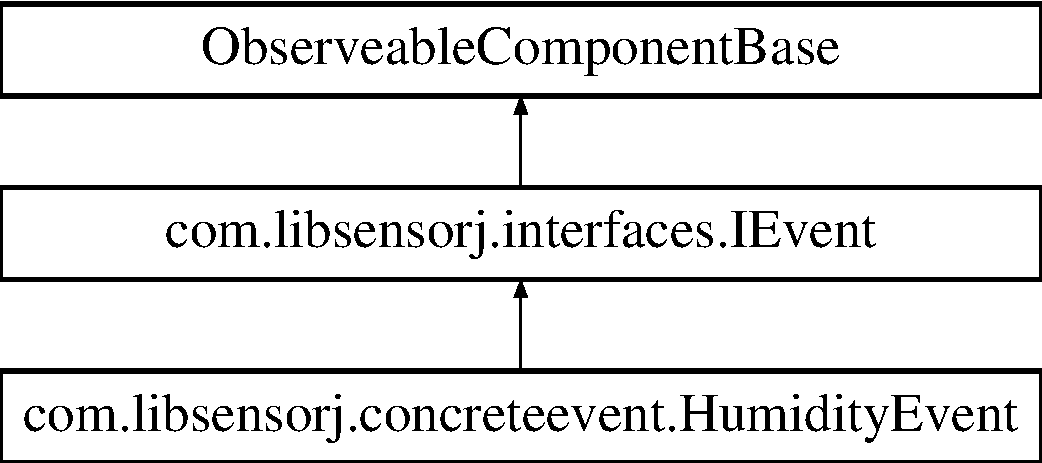
\includegraphics[height=2.000000cm]{classcom_1_1libsensorj_1_1concreteevent_1_1HumidityEvent}
\end{center}
\end{figure}
\subsection*{Public Member Functions}
\begin{DoxyCompactItemize}
\item 
void \hyperlink{classcom_1_1libsensorj_1_1concreteevent_1_1HumidityEvent_a4ea7f94d2402aeafca55dc1fb2950d00}{attach} (\hyperlink{classcom_1_1libsensorj_1_1model_1_1Observer}{Observer} obsever)
\item 
void \hyperlink{classcom_1_1libsensorj_1_1concreteevent_1_1HumidityEvent_a577a1f99a7993ccd8019fb46c1668c9b}{detach} (\hyperlink{classcom_1_1libsensorj_1_1model_1_1Observer}{Observer} obsever)
\item 
void \hyperlink{classcom_1_1libsensorj_1_1concreteevent_1_1HumidityEvent_ad3d8c57f1934c115f0c9374394d9a601}{trigger} ()
\end{DoxyCompactItemize}


\subsection{Member Function Documentation}
\hypertarget{classcom_1_1libsensorj_1_1concreteevent_1_1HumidityEvent_a4ea7f94d2402aeafca55dc1fb2950d00}{}\index{com\+::libsensorj\+::concreteevent\+::\+Humidity\+Event@{com\+::libsensorj\+::concreteevent\+::\+Humidity\+Event}!attach@{attach}}
\index{attach@{attach}!com\+::libsensorj\+::concreteevent\+::\+Humidity\+Event@{com\+::libsensorj\+::concreteevent\+::\+Humidity\+Event}}
\subsubsection[{attach}]{\setlength{\rightskip}{0pt plus 5cm}void com.\+libsensorj.\+concreteevent.\+Humidity\+Event.\+attach (
\begin{DoxyParamCaption}
\item[{{\bf Observer}}]{obsever}
\end{DoxyParamCaption}
)}\label{classcom_1_1libsensorj_1_1concreteevent_1_1HumidityEvent_a4ea7f94d2402aeafca55dc1fb2950d00}


Implements \hyperlink{interfacecom_1_1libsensorj_1_1interfaces_1_1IEvent_af5af4301ccb6670452419d68baddf372}{com.\+libsensorj.\+interfaces.\+I\+Event}.

\hypertarget{classcom_1_1libsensorj_1_1concreteevent_1_1HumidityEvent_a577a1f99a7993ccd8019fb46c1668c9b}{}\index{com\+::libsensorj\+::concreteevent\+::\+Humidity\+Event@{com\+::libsensorj\+::concreteevent\+::\+Humidity\+Event}!detach@{detach}}
\index{detach@{detach}!com\+::libsensorj\+::concreteevent\+::\+Humidity\+Event@{com\+::libsensorj\+::concreteevent\+::\+Humidity\+Event}}
\subsubsection[{detach}]{\setlength{\rightskip}{0pt plus 5cm}void com.\+libsensorj.\+concreteevent.\+Humidity\+Event.\+detach (
\begin{DoxyParamCaption}
\item[{{\bf Observer}}]{obsever}
\end{DoxyParamCaption}
)}\label{classcom_1_1libsensorj_1_1concreteevent_1_1HumidityEvent_a577a1f99a7993ccd8019fb46c1668c9b}


Implements \hyperlink{interfacecom_1_1libsensorj_1_1interfaces_1_1IEvent_a974b07df97fda9f3be8e4afcd46470b2}{com.\+libsensorj.\+interfaces.\+I\+Event}.

\hypertarget{classcom_1_1libsensorj_1_1concreteevent_1_1HumidityEvent_ad3d8c57f1934c115f0c9374394d9a601}{}\index{com\+::libsensorj\+::concreteevent\+::\+Humidity\+Event@{com\+::libsensorj\+::concreteevent\+::\+Humidity\+Event}!trigger@{trigger}}
\index{trigger@{trigger}!com\+::libsensorj\+::concreteevent\+::\+Humidity\+Event@{com\+::libsensorj\+::concreteevent\+::\+Humidity\+Event}}
\subsubsection[{trigger}]{\setlength{\rightskip}{0pt plus 5cm}void com.\+libsensorj.\+concreteevent.\+Humidity\+Event.\+trigger (
\begin{DoxyParamCaption}
{}
\end{DoxyParamCaption}
)}\label{classcom_1_1libsensorj_1_1concreteevent_1_1HumidityEvent_ad3d8c57f1934c115f0c9374394d9a601}


Implements \hyperlink{interfacecom_1_1libsensorj_1_1interfaces_1_1IEvent_a861dea0956f77dd82f95e0110b8043b2}{com.\+libsensorj.\+interfaces.\+I\+Event}.



The documentation for this class was generated from the following file\+:\begin{DoxyCompactItemize}
\item 
main/java/com/libsensorj/concreteevent/\hyperlink{HumidityEvent_8java}{Humidity\+Event.\+java}\end{DoxyCompactItemize}

\hypertarget{classcom_1_1libsensorj_1_1concretefactory_1_1HumiditySensorFactory}{}\section{com.\+libsensorj.\+concretefactory.\+Humidity\+Sensor\+Factory Class Reference}
\label{classcom_1_1libsensorj_1_1concretefactory_1_1HumiditySensorFactory}\index{com.\+libsensorj.\+concretefactory.\+Humidity\+Sensor\+Factory@{com.\+libsensorj.\+concretefactory.\+Humidity\+Sensor\+Factory}}
Inheritance diagram for com.\+libsensorj.\+concretefactory.\+Humidity\+Sensor\+Factory\+:\begin{figure}[H]
\begin{center}
\leavevmode
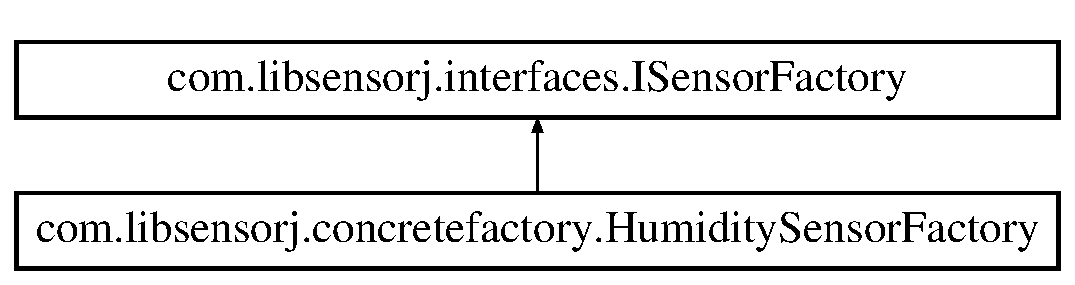
\includegraphics[height=2.000000cm]{classcom_1_1libsensorj_1_1concretefactory_1_1HumiditySensorFactory}
\end{center}
\end{figure}
\subsection*{Public Member Functions}
\begin{DoxyCompactItemize}
\item 
\hyperlink{interfacecom_1_1libsensorj_1_1interfaces_1_1ISensor}{I\+Sensor} \hyperlink{classcom_1_1libsensorj_1_1concretefactory_1_1HumiditySensorFactory_aec6f80bd08e69d69ea6187067d11d28c}{create\+Sensor} ()
\item 
\hyperlink{classcom_1_1libsensorj_1_1interfaces_1_1IEvent}{I\+Event} \hyperlink{classcom_1_1libsensorj_1_1concretefactory_1_1HumiditySensorFactory_a43835bfa4c60faf39dfe64f67322b9e4}{create\+Event} ()
\end{DoxyCompactItemize}


\subsection{Detailed Description}
A factory for creating Humidity\+Sensor objects. 

\subsection{Member Function Documentation}
\hypertarget{classcom_1_1libsensorj_1_1concretefactory_1_1HumiditySensorFactory_a43835bfa4c60faf39dfe64f67322b9e4}{}\index{com\+::libsensorj\+::concretefactory\+::\+Humidity\+Sensor\+Factory@{com\+::libsensorj\+::concretefactory\+::\+Humidity\+Sensor\+Factory}!create\+Event@{create\+Event}}
\index{create\+Event@{create\+Event}!com\+::libsensorj\+::concretefactory\+::\+Humidity\+Sensor\+Factory@{com\+::libsensorj\+::concretefactory\+::\+Humidity\+Sensor\+Factory}}
\subsubsection[{create\+Event}]{\setlength{\rightskip}{0pt plus 5cm}{\bf I\+Event} com.\+libsensorj.\+concretefactory.\+Humidity\+Sensor\+Factory.\+create\+Event (
\begin{DoxyParamCaption}
{}
\end{DoxyParamCaption}
)}\label{classcom_1_1libsensorj_1_1concretefactory_1_1HumiditySensorFactory_a43835bfa4c60faf39dfe64f67322b9e4}
Creates a new I\+Event object.

\begin{DoxyReturn}{Returns}
the I\+Event 
\end{DoxyReturn}


Implements \hyperlink{interfacecom_1_1libsensorj_1_1interfaces_1_1ISensorFactory_a2b074d01287a4e64677097255ba9e768}{com.\+libsensorj.\+interfaces.\+I\+Sensor\+Factory}.

\hypertarget{classcom_1_1libsensorj_1_1concretefactory_1_1HumiditySensorFactory_aec6f80bd08e69d69ea6187067d11d28c}{}\index{com\+::libsensorj\+::concretefactory\+::\+Humidity\+Sensor\+Factory@{com\+::libsensorj\+::concretefactory\+::\+Humidity\+Sensor\+Factory}!create\+Sensor@{create\+Sensor}}
\index{create\+Sensor@{create\+Sensor}!com\+::libsensorj\+::concretefactory\+::\+Humidity\+Sensor\+Factory@{com\+::libsensorj\+::concretefactory\+::\+Humidity\+Sensor\+Factory}}
\subsubsection[{create\+Sensor}]{\setlength{\rightskip}{0pt plus 5cm}{\bf I\+Sensor} com.\+libsensorj.\+concretefactory.\+Humidity\+Sensor\+Factory.\+create\+Sensor (
\begin{DoxyParamCaption}
{}
\end{DoxyParamCaption}
)}\label{classcom_1_1libsensorj_1_1concretefactory_1_1HumiditySensorFactory_aec6f80bd08e69d69ea6187067d11d28c}
Creates a new I\+Sensor object.

\begin{DoxyReturn}{Returns}
the I\+Sensor 
\end{DoxyReturn}


Implements \hyperlink{interfacecom_1_1libsensorj_1_1interfaces_1_1ISensorFactory_ac14c6d566c37c6a79c6db1e85634f25d}{com.\+libsensorj.\+interfaces.\+I\+Sensor\+Factory}.



The documentation for this class was generated from the following file\+:\begin{DoxyCompactItemize}
\item 
main/java/com/libsensorj/concretefactory/\hyperlink{HumiditySensorFactory_8java}{Humidity\+Sensor\+Factory.\+java}\end{DoxyCompactItemize}

\hypertarget{interfacecom_1_1libsensorj_1_1interfaces_1_1IActuator}{}\section{com.\+libsensorj.\+interfaces.\+I\+Actuator Interface Reference}
\label{interfacecom_1_1libsensorj_1_1interfaces_1_1IActuator}\index{com.\+libsensorj.\+interfaces.\+I\+Actuator@{com.\+libsensorj.\+interfaces.\+I\+Actuator}}
Inheritance diagram for com.\+libsensorj.\+interfaces.\+I\+Actuator\+:\begin{figure}[H]
\begin{center}
\leavevmode
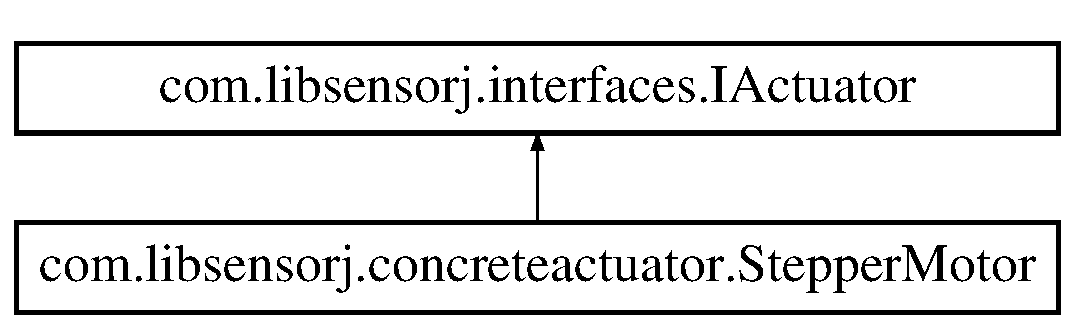
\includegraphics[height=2.000000cm]{interfacecom_1_1libsensorj_1_1interfaces_1_1IActuator}
\end{center}
\end{figure}


The documentation for this interface was generated from the following file\+:\begin{DoxyCompactItemize}
\item 
main/java/com/libsensorj/interfaces/\hyperlink{IActuator_8java}{I\+Actuator.\+java}\end{DoxyCompactItemize}

\hypertarget{classcom_1_1libsensorj_1_1interfaces_1_1IEvent}{}\section{com.\+libsensorj.\+interfaces.\+I\+Event Class Reference}
\label{classcom_1_1libsensorj_1_1interfaces_1_1IEvent}\index{com.\+libsensorj.\+interfaces.\+I\+Event@{com.\+libsensorj.\+interfaces.\+I\+Event}}
Inheritance diagram for com.\+libsensorj.\+interfaces.\+I\+Event\+:\begin{figure}[H]
\begin{center}
\leavevmode
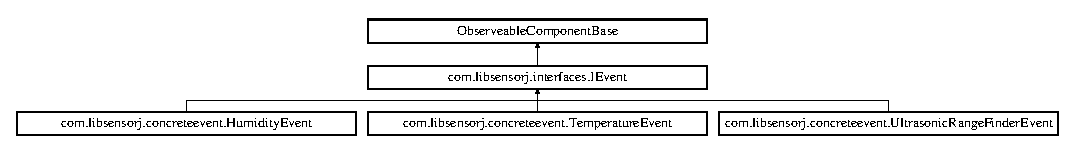
\includegraphics[height=1.595442cm]{classcom_1_1libsensorj_1_1interfaces_1_1IEvent}
\end{center}
\end{figure}
\subsection*{Public Member Functions}
\begin{DoxyCompactItemize}
\item 
abstract void \hyperlink{classcom_1_1libsensorj_1_1interfaces_1_1IEvent_a7e3cbdca3cceb9345483cf019760b113}{attach} (\hyperlink{classcom_1_1libsensorj_1_1model_1_1Observer}{Observer} obsever)
\item 
abstract void \hyperlink{classcom_1_1libsensorj_1_1interfaces_1_1IEvent_aae7d245feed8380465149bfa36724244}{detach} (\hyperlink{classcom_1_1libsensorj_1_1model_1_1Observer}{Observer} obsever)
\item 
abstract void \hyperlink{classcom_1_1libsensorj_1_1interfaces_1_1IEvent_aa12268158f158fbb805b558efeb1bb67}{trigger} ()
\end{DoxyCompactItemize}


\subsection{Detailed Description}
The Class \hyperlink{classcom_1_1libsensorj_1_1interfaces_1_1IEvent}{I\+Event}. 

\subsection{Member Function Documentation}
\hypertarget{classcom_1_1libsensorj_1_1interfaces_1_1IEvent_a7e3cbdca3cceb9345483cf019760b113}{}\index{com\+::libsensorj\+::interfaces\+::\+I\+Event@{com\+::libsensorj\+::interfaces\+::\+I\+Event}!attach@{attach}}
\index{attach@{attach}!com\+::libsensorj\+::interfaces\+::\+I\+Event@{com\+::libsensorj\+::interfaces\+::\+I\+Event}}
\subsubsection[{attach}]{\setlength{\rightskip}{0pt plus 5cm}abstract void com.\+libsensorj.\+interfaces.\+I\+Event.\+attach (
\begin{DoxyParamCaption}
\item[{{\bf Observer}}]{obsever}
\end{DoxyParamCaption}
)\hspace{0.3cm}{\ttfamily [abstract]}}\label{classcom_1_1libsensorj_1_1interfaces_1_1IEvent_a7e3cbdca3cceb9345483cf019760b113}
Attach.


\begin{DoxyParams}{Parameters}
{\em obsever} & the obsever \\
\hline
\end{DoxyParams}
\hypertarget{classcom_1_1libsensorj_1_1interfaces_1_1IEvent_aae7d245feed8380465149bfa36724244}{}\index{com\+::libsensorj\+::interfaces\+::\+I\+Event@{com\+::libsensorj\+::interfaces\+::\+I\+Event}!detach@{detach}}
\index{detach@{detach}!com\+::libsensorj\+::interfaces\+::\+I\+Event@{com\+::libsensorj\+::interfaces\+::\+I\+Event}}
\subsubsection[{detach}]{\setlength{\rightskip}{0pt plus 5cm}abstract void com.\+libsensorj.\+interfaces.\+I\+Event.\+detach (
\begin{DoxyParamCaption}
\item[{{\bf Observer}}]{obsever}
\end{DoxyParamCaption}
)\hspace{0.3cm}{\ttfamily [abstract]}}\label{classcom_1_1libsensorj_1_1interfaces_1_1IEvent_aae7d245feed8380465149bfa36724244}
Detach.


\begin{DoxyParams}{Parameters}
{\em obsever} & the obsever \\
\hline
\end{DoxyParams}
\hypertarget{classcom_1_1libsensorj_1_1interfaces_1_1IEvent_aa12268158f158fbb805b558efeb1bb67}{}\index{com\+::libsensorj\+::interfaces\+::\+I\+Event@{com\+::libsensorj\+::interfaces\+::\+I\+Event}!trigger@{trigger}}
\index{trigger@{trigger}!com\+::libsensorj\+::interfaces\+::\+I\+Event@{com\+::libsensorj\+::interfaces\+::\+I\+Event}}
\subsubsection[{trigger}]{\setlength{\rightskip}{0pt plus 5cm}abstract void com.\+libsensorj.\+interfaces.\+I\+Event.\+trigger (
\begin{DoxyParamCaption}
{}
\end{DoxyParamCaption}
)\hspace{0.3cm}{\ttfamily [abstract]}}\label{classcom_1_1libsensorj_1_1interfaces_1_1IEvent_aa12268158f158fbb805b558efeb1bb67}
Trigger. 

The documentation for this class was generated from the following file\+:\begin{DoxyCompactItemize}
\item 
main/java/com/libsensorj/interfaces/\hyperlink{IEvent_8java}{I\+Event.\+java}\end{DoxyCompactItemize}

\hypertarget{interfacecom_1_1libsensorj_1_1interfaces_1_1ISensor}{}\section{com.\+libsensorj.\+interfaces.\+I\+Sensor Interface Reference}
\label{interfacecom_1_1libsensorj_1_1interfaces_1_1ISensor}\index{com.\+libsensorj.\+interfaces.\+I\+Sensor@{com.\+libsensorj.\+interfaces.\+I\+Sensor}}
Inheritance diagram for com.\+libsensorj.\+interfaces.\+I\+Sensor\+:\begin{figure}[H]
\begin{center}
\leavevmode
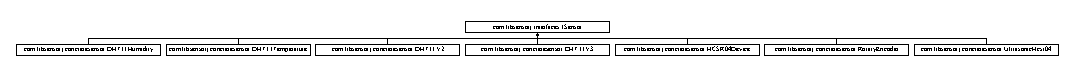
\includegraphics[height=1.216069cm]{interfacecom_1_1libsensorj_1_1interfaces_1_1ISensor}
\end{center}
\end{figure}
\subsection*{Public Member Functions}
\begin{DoxyCompactItemize}
\item 
void \hyperlink{interfacecom_1_1libsensorj_1_1interfaces_1_1ISensor_a3c3db93a33adecde81a528651790f75e}{get\+Instance} ()
\end{DoxyCompactItemize}


\subsection{Member Function Documentation}
\hypertarget{interfacecom_1_1libsensorj_1_1interfaces_1_1ISensor_a3c3db93a33adecde81a528651790f75e}{}\index{com\+::libsensorj\+::interfaces\+::\+I\+Sensor@{com\+::libsensorj\+::interfaces\+::\+I\+Sensor}!get\+Instance@{get\+Instance}}
\index{get\+Instance@{get\+Instance}!com\+::libsensorj\+::interfaces\+::\+I\+Sensor@{com\+::libsensorj\+::interfaces\+::\+I\+Sensor}}
\subsubsection[{get\+Instance}]{\setlength{\rightskip}{0pt plus 5cm}void com.\+libsensorj.\+interfaces.\+I\+Sensor.\+get\+Instance (
\begin{DoxyParamCaption}
{}
\end{DoxyParamCaption}
)}\label{interfacecom_1_1libsensorj_1_1interfaces_1_1ISensor_a3c3db93a33adecde81a528651790f75e}


Implemented in \hyperlink{classcom_1_1libsensorj_1_1concretesensor_1_1DHT11Temperature_a599358623598fb0076dc0a2e07978f0b}{com.\+libsensorj.\+concretesensor.\+D\+H\+T11\+Temperature}, \hyperlink{classcom_1_1libsensorj_1_1concretesensor_1_1UltrasonicHcsr04_a170167614b330d79518647a9a9722b62}{com.\+libsensorj.\+concretesensor.\+Ultrasonic\+Hcsr04}, and \hyperlink{classcom_1_1libsensorj_1_1concretesensor_1_1DHT11Humidity_a2355dc003abad8d519440e9f6871c422}{com.\+libsensorj.\+concretesensor.\+D\+H\+T11\+Humidity}.



The documentation for this interface was generated from the following file\+:\begin{DoxyCompactItemize}
\item 
main/java/com/libsensorj/interfaces/\hyperlink{ISensor_8java}{I\+Sensor.\+java}\end{DoxyCompactItemize}

\hypertarget{interfacecom_1_1libsensorj_1_1interfaces_1_1ISensorFactory}{}\section{com.\+libsensorj.\+interfaces.\+I\+Sensor\+Factory Interface Reference}
\label{interfacecom_1_1libsensorj_1_1interfaces_1_1ISensorFactory}\index{com.\+libsensorj.\+interfaces.\+I\+Sensor\+Factory@{com.\+libsensorj.\+interfaces.\+I\+Sensor\+Factory}}
Inheritance diagram for com.\+libsensorj.\+interfaces.\+I\+Sensor\+Factory\+:\begin{figure}[H]
\begin{center}
\leavevmode
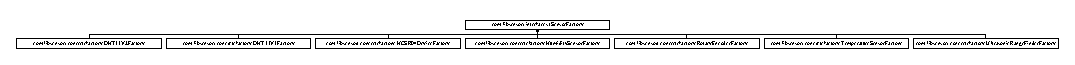
\includegraphics[height=0.430108cm]{interfacecom_1_1libsensorj_1_1interfaces_1_1ISensorFactory}
\end{center}
\end{figure}
\subsection*{Public Member Functions}
\begin{DoxyCompactItemize}
\item 
\hyperlink{interfacecom_1_1libsensorj_1_1interfaces_1_1ISensor}{I\+Sensor} \hyperlink{interfacecom_1_1libsensorj_1_1interfaces_1_1ISensorFactory_ac14c6d566c37c6a79c6db1e85634f25d}{create\+Sensor} ()
\item 
\hyperlink{classcom_1_1libsensorj_1_1interfaces_1_1IEvent}{I\+Event} \hyperlink{interfacecom_1_1libsensorj_1_1interfaces_1_1ISensorFactory_a2b074d01287a4e64677097255ba9e768}{create\+Event} ()
\end{DoxyCompactItemize}


\subsection{Detailed Description}
A factory for creating \hyperlink{interfacecom_1_1libsensorj_1_1interfaces_1_1ISensor}{I\+Sensor} objects. 

\subsection{Member Function Documentation}
\hypertarget{interfacecom_1_1libsensorj_1_1interfaces_1_1ISensorFactory_a2b074d01287a4e64677097255ba9e768}{}\index{com\+::libsensorj\+::interfaces\+::\+I\+Sensor\+Factory@{com\+::libsensorj\+::interfaces\+::\+I\+Sensor\+Factory}!create\+Event@{create\+Event}}
\index{create\+Event@{create\+Event}!com\+::libsensorj\+::interfaces\+::\+I\+Sensor\+Factory@{com\+::libsensorj\+::interfaces\+::\+I\+Sensor\+Factory}}
\subsubsection[{create\+Event}]{\setlength{\rightskip}{0pt plus 5cm}{\bf I\+Event} com.\+libsensorj.\+interfaces.\+I\+Sensor\+Factory.\+create\+Event (
\begin{DoxyParamCaption}
{}
\end{DoxyParamCaption}
)}\label{interfacecom_1_1libsensorj_1_1interfaces_1_1ISensorFactory_a2b074d01287a4e64677097255ba9e768}
Creates a new \hyperlink{classcom_1_1libsensorj_1_1interfaces_1_1IEvent}{I\+Event} object.

\begin{DoxyReturn}{Returns}
the \hyperlink{classcom_1_1libsensorj_1_1interfaces_1_1IEvent}{I\+Event} 
\end{DoxyReturn}


Implemented in \hyperlink{classcom_1_1libsensorj_1_1concretefactory_1_1DHT11V2Factory_a0eb0b480f4133c3eeb2728bd0fa45c58}{com.\+libsensorj.\+concretefactory.\+D\+H\+T11\+V2\+Factory}, \hyperlink{classcom_1_1libsensorj_1_1concretefactory_1_1TemperatureSensorFactory_adb3d5716b5e55f4fc037c0a95ec99688}{com.\+libsensorj.\+concretefactory.\+Temperature\+Sensor\+Factory}, \hyperlink{classcom_1_1libsensorj_1_1concretefactory_1_1HumiditySensorFactory_a43835bfa4c60faf39dfe64f67322b9e4}{com.\+libsensorj.\+concretefactory.\+Humidity\+Sensor\+Factory}, \hyperlink{classcom_1_1libsensorj_1_1concretefactory_1_1DHT11V3Factory_a7621f6dc5c877e6dfb160f68e50fd319}{com.\+libsensorj.\+concretefactory.\+D\+H\+T11\+V3\+Factory}, \hyperlink{classcom_1_1libsensorj_1_1concretefactory_1_1HCSR04DeviceFactory_aea88b0202d3021c4e55bd9cbf64da906}{com.\+libsensorj.\+concretefactory.\+H\+C\+S\+R04\+Device\+Factory}, \hyperlink{classcom_1_1libsensorj_1_1concretefactory_1_1UltrasonicRangeFinderFactory_a8a7d0c55346f1ab5630a878f6a3175fd}{com.\+libsensorj.\+concretefactory.\+Ultrasonic\+Range\+Finder\+Factory}, and \hyperlink{classcom_1_1libsensorj_1_1concretefactory_1_1RotaryEncoderFactory_a8f36c2cbdddcd1c71d438efafc73ffc2}{com.\+libsensorj.\+concretefactory.\+Rotary\+Encoder\+Factory}.

\hypertarget{interfacecom_1_1libsensorj_1_1interfaces_1_1ISensorFactory_ac14c6d566c37c6a79c6db1e85634f25d}{}\index{com\+::libsensorj\+::interfaces\+::\+I\+Sensor\+Factory@{com\+::libsensorj\+::interfaces\+::\+I\+Sensor\+Factory}!create\+Sensor@{create\+Sensor}}
\index{create\+Sensor@{create\+Sensor}!com\+::libsensorj\+::interfaces\+::\+I\+Sensor\+Factory@{com\+::libsensorj\+::interfaces\+::\+I\+Sensor\+Factory}}
\subsubsection[{create\+Sensor}]{\setlength{\rightskip}{0pt plus 5cm}{\bf I\+Sensor} com.\+libsensorj.\+interfaces.\+I\+Sensor\+Factory.\+create\+Sensor (
\begin{DoxyParamCaption}
{}
\end{DoxyParamCaption}
)}\label{interfacecom_1_1libsensorj_1_1interfaces_1_1ISensorFactory_ac14c6d566c37c6a79c6db1e85634f25d}
Creates a new \hyperlink{interfacecom_1_1libsensorj_1_1interfaces_1_1ISensor}{I\+Sensor} object.

\begin{DoxyReturn}{Returns}
the \hyperlink{interfacecom_1_1libsensorj_1_1interfaces_1_1ISensor}{I\+Sensor} 
\end{DoxyReturn}


Implemented in \hyperlink{classcom_1_1libsensorj_1_1concretefactory_1_1DHT11V2Factory_ac04eaebc748d420eb035439dfc1d2202}{com.\+libsensorj.\+concretefactory.\+D\+H\+T11\+V2\+Factory}, \hyperlink{classcom_1_1libsensorj_1_1concretefactory_1_1DHT11V3Factory_ad89c967025d654490729d2f69438805e}{com.\+libsensorj.\+concretefactory.\+D\+H\+T11\+V3\+Factory}, \hyperlink{classcom_1_1libsensorj_1_1concretefactory_1_1HCSR04DeviceFactory_a3d5c07b9ce458a3f56cfe5e7470b51df}{com.\+libsensorj.\+concretefactory.\+H\+C\+S\+R04\+Device\+Factory}, \hyperlink{classcom_1_1libsensorj_1_1concretefactory_1_1HumiditySensorFactory_aec6f80bd08e69d69ea6187067d11d28c}{com.\+libsensorj.\+concretefactory.\+Humidity\+Sensor\+Factory}, \hyperlink{classcom_1_1libsensorj_1_1concretefactory_1_1TemperatureSensorFactory_aeba8598ebe5c182154f63e0c94abdd70}{com.\+libsensorj.\+concretefactory.\+Temperature\+Sensor\+Factory}, \hyperlink{classcom_1_1libsensorj_1_1concretefactory_1_1UltrasonicRangeFinderFactory_a3aa6e46ef47bf97355df4d5cfb1b1e01}{com.\+libsensorj.\+concretefactory.\+Ultrasonic\+Range\+Finder\+Factory}, and \hyperlink{classcom_1_1libsensorj_1_1concretefactory_1_1RotaryEncoderFactory_a5f9c404d9b61d8aaf63cad82b87becd7}{com.\+libsensorj.\+concretefactory.\+Rotary\+Encoder\+Factory}.



The documentation for this interface was generated from the following file\+:\begin{DoxyCompactItemize}
\item 
main/java/com/libsensorj/interfaces/\hyperlink{ISensorFactory_8java}{I\+Sensor\+Factory.\+java}\end{DoxyCompactItemize}

\hypertarget{interfacecom_1_1libsensorj_1_1concreteactuator_1_1interfaces_1_1IStepperMotor}{}\section{com.\+libsensorj.\+concreteactuator.\+interfaces.\+I\+Stepper\+Motor Interface Reference}
\label{interfacecom_1_1libsensorj_1_1concreteactuator_1_1interfaces_1_1IStepperMotor}\index{com.\+libsensorj.\+concreteactuator.\+interfaces.\+I\+Stepper\+Motor@{com.\+libsensorj.\+concreteactuator.\+interfaces.\+I\+Stepper\+Motor}}
Inheritance diagram for com.\+libsensorj.\+concreteactuator.\+interfaces.\+I\+Stepper\+Motor\+:\begin{figure}[H]
\begin{center}
\leavevmode
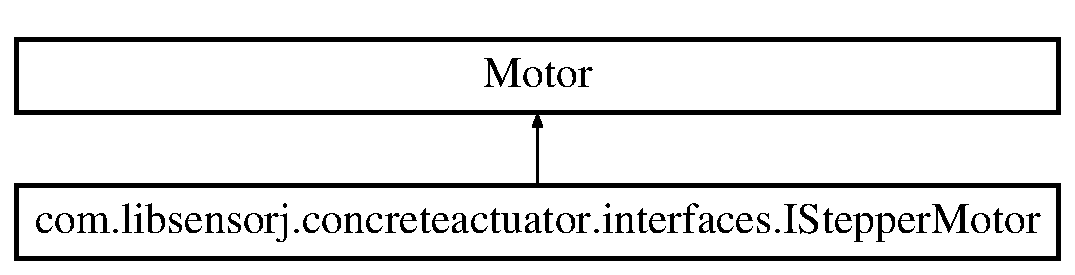
\includegraphics[height=2.000000cm]{interfacecom_1_1libsensorj_1_1concreteactuator_1_1interfaces_1_1IStepperMotor}
\end{center}
\end{figure}
\subsection*{Public Member Functions}
\begin{DoxyCompactItemize}
\item 
float \hyperlink{interfacecom_1_1libsensorj_1_1concreteactuator_1_1interfaces_1_1IStepperMotor_afc7fc6ed71c0098df44dc97d051bba74}{get\+Steps\+Per\+Revolution} ()
\item 
void \hyperlink{interfacecom_1_1libsensorj_1_1concreteactuator_1_1interfaces_1_1IStepperMotor_a5c136c6767e43b652286468529c66e58}{set\+Steps\+Per\+Revolution} (int steps)
\item 
void \hyperlink{interfacecom_1_1libsensorj_1_1concreteactuator_1_1interfaces_1_1IStepperMotor_a4894a4c5917bfa66db31b3cb0342ad25}{set\+Step\+Interval} (long milliseconds)
\item 
void \hyperlink{interfacecom_1_1libsensorj_1_1concreteactuator_1_1interfaces_1_1IStepperMotor_a0772dc757e0281f612de513066515296}{set\+Step\+Interval} (long milliseconds, int nanoseconds)
\item 
void \hyperlink{interfacecom_1_1libsensorj_1_1concreteactuator_1_1interfaces_1_1IStepperMotor_ae771f40d126e2251f4043b11340be57b}{set\+Step\+Sequence} (byte\mbox{[}$\,$\mbox{]} sequence)
\item 
byte\mbox{[}$\,$\mbox{]} \hyperlink{interfacecom_1_1libsensorj_1_1concreteactuator_1_1interfaces_1_1IStepperMotor_a878ca81b5a32fbed1a52e9605b61818a}{get\+Step\+Sequence} ()
\item 
void \hyperlink{interfacecom_1_1libsensorj_1_1concreteactuator_1_1interfaces_1_1IStepperMotor_ae3f5dbdba759ed2efe4d5195f9aae2a1}{rotate} (double revolutions)
\item 
void \hyperlink{interfacecom_1_1libsensorj_1_1concreteactuator_1_1interfaces_1_1IStepperMotor_af93fff3068238b5222df10d50e2983ac}{step} (long steps)
\end{DoxyCompactItemize}


\subsection{Member Function Documentation}
\hypertarget{interfacecom_1_1libsensorj_1_1concreteactuator_1_1interfaces_1_1IStepperMotor_a878ca81b5a32fbed1a52e9605b61818a}{}\index{com\+::libsensorj\+::concreteactuator\+::interfaces\+::\+I\+Stepper\+Motor@{com\+::libsensorj\+::concreteactuator\+::interfaces\+::\+I\+Stepper\+Motor}!get\+Step\+Sequence@{get\+Step\+Sequence}}
\index{get\+Step\+Sequence@{get\+Step\+Sequence}!com\+::libsensorj\+::concreteactuator\+::interfaces\+::\+I\+Stepper\+Motor@{com\+::libsensorj\+::concreteactuator\+::interfaces\+::\+I\+Stepper\+Motor}}
\subsubsection[{get\+Step\+Sequence}]{\setlength{\rightskip}{0pt plus 5cm}byte \mbox{[}$\,$\mbox{]} com.\+libsensorj.\+concreteactuator.\+interfaces.\+I\+Stepper\+Motor.\+get\+Step\+Sequence (
\begin{DoxyParamCaption}
{}
\end{DoxyParamCaption}
)}\label{interfacecom_1_1libsensorj_1_1concreteactuator_1_1interfaces_1_1IStepperMotor_a878ca81b5a32fbed1a52e9605b61818a}
\hypertarget{interfacecom_1_1libsensorj_1_1concreteactuator_1_1interfaces_1_1IStepperMotor_afc7fc6ed71c0098df44dc97d051bba74}{}\index{com\+::libsensorj\+::concreteactuator\+::interfaces\+::\+I\+Stepper\+Motor@{com\+::libsensorj\+::concreteactuator\+::interfaces\+::\+I\+Stepper\+Motor}!get\+Steps\+Per\+Revolution@{get\+Steps\+Per\+Revolution}}
\index{get\+Steps\+Per\+Revolution@{get\+Steps\+Per\+Revolution}!com\+::libsensorj\+::concreteactuator\+::interfaces\+::\+I\+Stepper\+Motor@{com\+::libsensorj\+::concreteactuator\+::interfaces\+::\+I\+Stepper\+Motor}}
\subsubsection[{get\+Steps\+Per\+Revolution}]{\setlength{\rightskip}{0pt plus 5cm}float com.\+libsensorj.\+concreteactuator.\+interfaces.\+I\+Stepper\+Motor.\+get\+Steps\+Per\+Revolution (
\begin{DoxyParamCaption}
{}
\end{DoxyParamCaption}
)}\label{interfacecom_1_1libsensorj_1_1concreteactuator_1_1interfaces_1_1IStepperMotor_afc7fc6ed71c0098df44dc97d051bba74}
\hypertarget{interfacecom_1_1libsensorj_1_1concreteactuator_1_1interfaces_1_1IStepperMotor_ae3f5dbdba759ed2efe4d5195f9aae2a1}{}\index{com\+::libsensorj\+::concreteactuator\+::interfaces\+::\+I\+Stepper\+Motor@{com\+::libsensorj\+::concreteactuator\+::interfaces\+::\+I\+Stepper\+Motor}!rotate@{rotate}}
\index{rotate@{rotate}!com\+::libsensorj\+::concreteactuator\+::interfaces\+::\+I\+Stepper\+Motor@{com\+::libsensorj\+::concreteactuator\+::interfaces\+::\+I\+Stepper\+Motor}}
\subsubsection[{rotate}]{\setlength{\rightskip}{0pt plus 5cm}void com.\+libsensorj.\+concreteactuator.\+interfaces.\+I\+Stepper\+Motor.\+rotate (
\begin{DoxyParamCaption}
\item[{double}]{revolutions}
\end{DoxyParamCaption}
)}\label{interfacecom_1_1libsensorj_1_1concreteactuator_1_1interfaces_1_1IStepperMotor_ae3f5dbdba759ed2efe4d5195f9aae2a1}
\hypertarget{interfacecom_1_1libsensorj_1_1concreteactuator_1_1interfaces_1_1IStepperMotor_a4894a4c5917bfa66db31b3cb0342ad25}{}\index{com\+::libsensorj\+::concreteactuator\+::interfaces\+::\+I\+Stepper\+Motor@{com\+::libsensorj\+::concreteactuator\+::interfaces\+::\+I\+Stepper\+Motor}!set\+Step\+Interval@{set\+Step\+Interval}}
\index{set\+Step\+Interval@{set\+Step\+Interval}!com\+::libsensorj\+::concreteactuator\+::interfaces\+::\+I\+Stepper\+Motor@{com\+::libsensorj\+::concreteactuator\+::interfaces\+::\+I\+Stepper\+Motor}}
\subsubsection[{set\+Step\+Interval}]{\setlength{\rightskip}{0pt plus 5cm}void com.\+libsensorj.\+concreteactuator.\+interfaces.\+I\+Stepper\+Motor.\+set\+Step\+Interval (
\begin{DoxyParamCaption}
\item[{long}]{milliseconds}
\end{DoxyParamCaption}
)}\label{interfacecom_1_1libsensorj_1_1concreteactuator_1_1interfaces_1_1IStepperMotor_a4894a4c5917bfa66db31b3cb0342ad25}
\hypertarget{interfacecom_1_1libsensorj_1_1concreteactuator_1_1interfaces_1_1IStepperMotor_a0772dc757e0281f612de513066515296}{}\index{com\+::libsensorj\+::concreteactuator\+::interfaces\+::\+I\+Stepper\+Motor@{com\+::libsensorj\+::concreteactuator\+::interfaces\+::\+I\+Stepper\+Motor}!set\+Step\+Interval@{set\+Step\+Interval}}
\index{set\+Step\+Interval@{set\+Step\+Interval}!com\+::libsensorj\+::concreteactuator\+::interfaces\+::\+I\+Stepper\+Motor@{com\+::libsensorj\+::concreteactuator\+::interfaces\+::\+I\+Stepper\+Motor}}
\subsubsection[{set\+Step\+Interval}]{\setlength{\rightskip}{0pt plus 5cm}void com.\+libsensorj.\+concreteactuator.\+interfaces.\+I\+Stepper\+Motor.\+set\+Step\+Interval (
\begin{DoxyParamCaption}
\item[{long}]{milliseconds, }
\item[{int}]{nanoseconds}
\end{DoxyParamCaption}
)}\label{interfacecom_1_1libsensorj_1_1concreteactuator_1_1interfaces_1_1IStepperMotor_a0772dc757e0281f612de513066515296}
\hypertarget{interfacecom_1_1libsensorj_1_1concreteactuator_1_1interfaces_1_1IStepperMotor_ae771f40d126e2251f4043b11340be57b}{}\index{com\+::libsensorj\+::concreteactuator\+::interfaces\+::\+I\+Stepper\+Motor@{com\+::libsensorj\+::concreteactuator\+::interfaces\+::\+I\+Stepper\+Motor}!set\+Step\+Sequence@{set\+Step\+Sequence}}
\index{set\+Step\+Sequence@{set\+Step\+Sequence}!com\+::libsensorj\+::concreteactuator\+::interfaces\+::\+I\+Stepper\+Motor@{com\+::libsensorj\+::concreteactuator\+::interfaces\+::\+I\+Stepper\+Motor}}
\subsubsection[{set\+Step\+Sequence}]{\setlength{\rightskip}{0pt plus 5cm}void com.\+libsensorj.\+concreteactuator.\+interfaces.\+I\+Stepper\+Motor.\+set\+Step\+Sequence (
\begin{DoxyParamCaption}
\item[{byte\mbox{[}$\,$\mbox{]}}]{sequence}
\end{DoxyParamCaption}
)}\label{interfacecom_1_1libsensorj_1_1concreteactuator_1_1interfaces_1_1IStepperMotor_ae771f40d126e2251f4043b11340be57b}
\hypertarget{interfacecom_1_1libsensorj_1_1concreteactuator_1_1interfaces_1_1IStepperMotor_a5c136c6767e43b652286468529c66e58}{}\index{com\+::libsensorj\+::concreteactuator\+::interfaces\+::\+I\+Stepper\+Motor@{com\+::libsensorj\+::concreteactuator\+::interfaces\+::\+I\+Stepper\+Motor}!set\+Steps\+Per\+Revolution@{set\+Steps\+Per\+Revolution}}
\index{set\+Steps\+Per\+Revolution@{set\+Steps\+Per\+Revolution}!com\+::libsensorj\+::concreteactuator\+::interfaces\+::\+I\+Stepper\+Motor@{com\+::libsensorj\+::concreteactuator\+::interfaces\+::\+I\+Stepper\+Motor}}
\subsubsection[{set\+Steps\+Per\+Revolution}]{\setlength{\rightskip}{0pt plus 5cm}void com.\+libsensorj.\+concreteactuator.\+interfaces.\+I\+Stepper\+Motor.\+set\+Steps\+Per\+Revolution (
\begin{DoxyParamCaption}
\item[{int}]{steps}
\end{DoxyParamCaption}
)}\label{interfacecom_1_1libsensorj_1_1concreteactuator_1_1interfaces_1_1IStepperMotor_a5c136c6767e43b652286468529c66e58}
\hypertarget{interfacecom_1_1libsensorj_1_1concreteactuator_1_1interfaces_1_1IStepperMotor_af93fff3068238b5222df10d50e2983ac}{}\index{com\+::libsensorj\+::concreteactuator\+::interfaces\+::\+I\+Stepper\+Motor@{com\+::libsensorj\+::concreteactuator\+::interfaces\+::\+I\+Stepper\+Motor}!step@{step}}
\index{step@{step}!com\+::libsensorj\+::concreteactuator\+::interfaces\+::\+I\+Stepper\+Motor@{com\+::libsensorj\+::concreteactuator\+::interfaces\+::\+I\+Stepper\+Motor}}
\subsubsection[{step}]{\setlength{\rightskip}{0pt plus 5cm}void com.\+libsensorj.\+concreteactuator.\+interfaces.\+I\+Stepper\+Motor.\+step (
\begin{DoxyParamCaption}
\item[{long}]{steps}
\end{DoxyParamCaption}
)}\label{interfacecom_1_1libsensorj_1_1concreteactuator_1_1interfaces_1_1IStepperMotor_af93fff3068238b5222df10d50e2983ac}


The documentation for this interface was generated from the following file\+:\begin{DoxyCompactItemize}
\item 
main/java/com/libsensorj/concreteactuator/interfaces/\hyperlink{IStepperMotor_8java}{I\+Stepper\+Motor.\+java}\end{DoxyCompactItemize}

\hypertarget{classcom_1_1libsensorj_1_1utils_1_1LibPins}{}\section{com.\+libsensorj.\+utils.\+Lib\+Pins Class Reference}
\label{classcom_1_1libsensorj_1_1utils_1_1LibPins}\index{com.\+libsensorj.\+utils.\+Lib\+Pins@{com.\+libsensorj.\+utils.\+Lib\+Pins}}
\subsection*{Static Public Member Functions}
\begin{DoxyCompactItemize}
\item 
static Pin \hyperlink{classcom_1_1libsensorj_1_1utils_1_1LibPins_ad30688404fa1f82b0ef038bc967255c3}{get\+Pin} (int pin\+Number)
\end{DoxyCompactItemize}
\subsection*{Static Package Functions}
\begin{DoxyCompactItemize}
\item 
\hyperlink{classcom_1_1libsensorj_1_1utils_1_1LibPins_a219d56076453e22e5971cfaaf50c70b1}{\mbox{[}static initializer\mbox{]}}
\end{DoxyCompactItemize}
\subsection*{Static Private Attributes}
\begin{DoxyCompactItemize}
\item 
static Map$<$ Integer, Pin $>$ \hyperlink{classcom_1_1libsensorj_1_1utils_1_1LibPins_a46bbd1e6636d9dc4f95d65a38ef33d5d}{gpio\+Pins}
\end{DoxyCompactItemize}


\subsection{Detailed Description}
The Class \hyperlink{classcom_1_1libsensorj_1_1utils_1_1LibPins}{Lib\+Pins}. 

\subsection{Member Function Documentation}
\hypertarget{classcom_1_1libsensorj_1_1utils_1_1LibPins_a219d56076453e22e5971cfaaf50c70b1}{}\index{com\+::libsensorj\+::utils\+::\+Lib\+Pins@{com\+::libsensorj\+::utils\+::\+Lib\+Pins}!\mbox{[}static initializer\mbox{]}@{[static initializer]}}
\index{\mbox{[}static initializer\mbox{]}@{[static initializer]}!com\+::libsensorj\+::utils\+::\+Lib\+Pins@{com\+::libsensorj\+::utils\+::\+Lib\+Pins}}
\subsubsection[{[static initializer]}]{\setlength{\rightskip}{0pt plus 5cm}com.\+libsensorj.\+utils.\+Lib\+Pins.\mbox{[}static initializer\mbox{]} (
\begin{DoxyParamCaption}
{}
\end{DoxyParamCaption}
)\hspace{0.3cm}{\ttfamily [static]}, {\ttfamily [package]}}\label{classcom_1_1libsensorj_1_1utils_1_1LibPins_a219d56076453e22e5971cfaaf50c70b1}
\hypertarget{classcom_1_1libsensorj_1_1utils_1_1LibPins_ad30688404fa1f82b0ef038bc967255c3}{}\index{com\+::libsensorj\+::utils\+::\+Lib\+Pins@{com\+::libsensorj\+::utils\+::\+Lib\+Pins}!get\+Pin@{get\+Pin}}
\index{get\+Pin@{get\+Pin}!com\+::libsensorj\+::utils\+::\+Lib\+Pins@{com\+::libsensorj\+::utils\+::\+Lib\+Pins}}
\subsubsection[{get\+Pin}]{\setlength{\rightskip}{0pt plus 5cm}static Pin com.\+libsensorj.\+utils.\+Lib\+Pins.\+get\+Pin (
\begin{DoxyParamCaption}
\item[{int}]{pin\+Number}
\end{DoxyParamCaption}
)\hspace{0.3cm}{\ttfamily [static]}}\label{classcom_1_1libsensorj_1_1utils_1_1LibPins_ad30688404fa1f82b0ef038bc967255c3}
Gets the pin.


\begin{DoxyParams}{Parameters}
{\em pin\+Number} & the pin number \\
\hline
\end{DoxyParams}
\begin{DoxyReturn}{Returns}
the pin 
\end{DoxyReturn}


\subsection{Member Data Documentation}
\hypertarget{classcom_1_1libsensorj_1_1utils_1_1LibPins_a46bbd1e6636d9dc4f95d65a38ef33d5d}{}\index{com\+::libsensorj\+::utils\+::\+Lib\+Pins@{com\+::libsensorj\+::utils\+::\+Lib\+Pins}!gpio\+Pins@{gpio\+Pins}}
\index{gpio\+Pins@{gpio\+Pins}!com\+::libsensorj\+::utils\+::\+Lib\+Pins@{com\+::libsensorj\+::utils\+::\+Lib\+Pins}}
\subsubsection[{gpio\+Pins}]{\setlength{\rightskip}{0pt plus 5cm}Map$<$Integer, Pin$>$ com.\+libsensorj.\+utils.\+Lib\+Pins.\+gpio\+Pins\hspace{0.3cm}{\ttfamily [static]}, {\ttfamily [private]}}\label{classcom_1_1libsensorj_1_1utils_1_1LibPins_a46bbd1e6636d9dc4f95d65a38ef33d5d}
The gpio pins. 

The documentation for this class was generated from the following file\+:\begin{DoxyCompactItemize}
\item 
main/java/com/libsensorj/utils/\hyperlink{LibPins_8java}{Lib\+Pins.\+java}\end{DoxyCompactItemize}

\hypertarget{classcom_1_1libsensorj_1_1mock_1_1MockGpioFactory}{}\section{com.\+libsensorj.\+mock.\+Mock\+Gpio\+Factory Class Reference}
\label{classcom_1_1libsensorj_1_1mock_1_1MockGpioFactory}\index{com.\+libsensorj.\+mock.\+Mock\+Gpio\+Factory@{com.\+libsensorj.\+mock.\+Mock\+Gpio\+Factory}}
\subsection*{Static Public Member Functions}
\begin{DoxyCompactItemize}
\item 
static Gpio\+Controller \hyperlink{classcom_1_1libsensorj_1_1mock_1_1MockGpioFactory_a58463148954717dc22f75886523d4771}{get\+Instance} ()
\item 
static \hyperlink{classcom_1_1libsensorj_1_1mock_1_1MockGpioProvider}{Mock\+Gpio\+Provider} \hyperlink{classcom_1_1libsensorj_1_1mock_1_1MockGpioFactory_adbc2afeac5d0b886eef76f1984f0c382}{get\+Mock\+Provider} ()
\end{DoxyCompactItemize}
\subsection*{Private Member Functions}
\begin{DoxyCompactItemize}
\item 
\hyperlink{classcom_1_1libsensorj_1_1mock_1_1MockGpioFactory_ad4fb10cfe04911a6104bbb1e0b3a3252}{Mock\+Gpio\+Factory} ()
\end{DoxyCompactItemize}
\subsection*{Static Private Attributes}
\begin{DoxyCompactItemize}
\item 
static \hyperlink{classcom_1_1libsensorj_1_1mock_1_1MockGpioProvider}{Mock\+Gpio\+Provider} \hyperlink{classcom_1_1libsensorj_1_1mock_1_1MockGpioFactory_aa7cf0e5787b3ffe138f0cea0668df93e}{provider} = null
\end{DoxyCompactItemize}


\subsection{Detailed Description}
This factory class provides a static method to create new 'Gpio\+Controller' instances. 

Before using the Pi4\+J library, you need to ensure that the Java V\+M in configured with access to the following system libraries\+: 
\begin{DoxyItemize}
\item \hyperlink{namespacecom_1_1pi4j}{pi4j} 
\item wiring\+Pi 
\end{DoxyItemize}\begin{quote}
This library depends on the wiring\+Pi native system library. (developed by Gordon Henderson @ \href{https://projects.drogon.net/}{\tt https\+://projects.\+drogon.\+net/}) \end{quote}


\begin{DoxyAuthor}{Author}
Robert Savage (\href{http://www.savagehomeautomation.com}{\tt http\+://www .savagehomeautomation.\+com}) 
\end{DoxyAuthor}
\begin{DoxySeeAlso}{See also}
\hyperlink{namespacecom}{com} 

\href{http://www.pi4j.com/}{\tt http\+://www.\+pi4j.\+com/} 
\end{DoxySeeAlso}


\subsection{Constructor \& Destructor Documentation}
\hypertarget{classcom_1_1libsensorj_1_1mock_1_1MockGpioFactory_ad4fb10cfe04911a6104bbb1e0b3a3252}{}\index{com\+::libsensorj\+::mock\+::\+Mock\+Gpio\+Factory@{com\+::libsensorj\+::mock\+::\+Mock\+Gpio\+Factory}!Mock\+Gpio\+Factory@{Mock\+Gpio\+Factory}}
\index{Mock\+Gpio\+Factory@{Mock\+Gpio\+Factory}!com\+::libsensorj\+::mock\+::\+Mock\+Gpio\+Factory@{com\+::libsensorj\+::mock\+::\+Mock\+Gpio\+Factory}}
\subsubsection[{Mock\+Gpio\+Factory}]{\setlength{\rightskip}{0pt plus 5cm}com.\+libsensorj.\+mock.\+Mock\+Gpio\+Factory.\+Mock\+Gpio\+Factory (
\begin{DoxyParamCaption}
{}
\end{DoxyParamCaption}
)\hspace{0.3cm}{\ttfamily [private]}}\label{classcom_1_1libsensorj_1_1mock_1_1MockGpioFactory_ad4fb10cfe04911a6104bbb1e0b3a3252}
Instantiates a new mock gpio factory. 

\subsection{Member Function Documentation}
\hypertarget{classcom_1_1libsensorj_1_1mock_1_1MockGpioFactory_a58463148954717dc22f75886523d4771}{}\index{com\+::libsensorj\+::mock\+::\+Mock\+Gpio\+Factory@{com\+::libsensorj\+::mock\+::\+Mock\+Gpio\+Factory}!get\+Instance@{get\+Instance}}
\index{get\+Instance@{get\+Instance}!com\+::libsensorj\+::mock\+::\+Mock\+Gpio\+Factory@{com\+::libsensorj\+::mock\+::\+Mock\+Gpio\+Factory}}
\subsubsection[{get\+Instance}]{\setlength{\rightskip}{0pt plus 5cm}static Gpio\+Controller com.\+libsensorj.\+mock.\+Mock\+Gpio\+Factory.\+get\+Instance (
\begin{DoxyParamCaption}
{}
\end{DoxyParamCaption}
)\hspace{0.3cm}{\ttfamily [static]}}\label{classcom_1_1libsensorj_1_1mock_1_1MockGpioFactory_a58463148954717dc22f75886523d4771}
Create New G\+P\+I\+O Controller instance.

\begin{DoxyReturn}{Returns}
Return a new Gpio\+Controller impl instance. 
\end{DoxyReturn}
\hypertarget{classcom_1_1libsensorj_1_1mock_1_1MockGpioFactory_adbc2afeac5d0b886eef76f1984f0c382}{}\index{com\+::libsensorj\+::mock\+::\+Mock\+Gpio\+Factory@{com\+::libsensorj\+::mock\+::\+Mock\+Gpio\+Factory}!get\+Mock\+Provider@{get\+Mock\+Provider}}
\index{get\+Mock\+Provider@{get\+Mock\+Provider}!com\+::libsensorj\+::mock\+::\+Mock\+Gpio\+Factory@{com\+::libsensorj\+::mock\+::\+Mock\+Gpio\+Factory}}
\subsubsection[{get\+Mock\+Provider}]{\setlength{\rightskip}{0pt plus 5cm}static {\bf Mock\+Gpio\+Provider} com.\+libsensorj.\+mock.\+Mock\+Gpio\+Factory.\+get\+Mock\+Provider (
\begin{DoxyParamCaption}
{}
\end{DoxyParamCaption}
)\hspace{0.3cm}{\ttfamily [static]}}\label{classcom_1_1libsensorj_1_1mock_1_1MockGpioFactory_adbc2afeac5d0b886eef76f1984f0c382}
Gets the mock provider.

\begin{DoxyReturn}{Returns}
the mock provider 
\end{DoxyReturn}


\subsection{Member Data Documentation}
\hypertarget{classcom_1_1libsensorj_1_1mock_1_1MockGpioFactory_aa7cf0e5787b3ffe138f0cea0668df93e}{}\index{com\+::libsensorj\+::mock\+::\+Mock\+Gpio\+Factory@{com\+::libsensorj\+::mock\+::\+Mock\+Gpio\+Factory}!provider@{provider}}
\index{provider@{provider}!com\+::libsensorj\+::mock\+::\+Mock\+Gpio\+Factory@{com\+::libsensorj\+::mock\+::\+Mock\+Gpio\+Factory}}
\subsubsection[{provider}]{\setlength{\rightskip}{0pt plus 5cm}{\bf Mock\+Gpio\+Provider} com.\+libsensorj.\+mock.\+Mock\+Gpio\+Factory.\+provider = null\hspace{0.3cm}{\ttfamily [static]}, {\ttfamily [private]}}\label{classcom_1_1libsensorj_1_1mock_1_1MockGpioFactory_aa7cf0e5787b3ffe138f0cea0668df93e}
The provider. 

The documentation for this class was generated from the following file\+:\begin{DoxyCompactItemize}
\item 
test/java/com/libsensorj/mock/\hyperlink{MockGpioFactory_8java}{Mock\+Gpio\+Factory.\+java}\end{DoxyCompactItemize}

\hypertarget{classcom_1_1libsensorj_1_1mock_1_1MockGpioProvider}{}\section{com.\+libsensorj.\+mock.\+Mock\+Gpio\+Provider Class Reference}
\label{classcom_1_1libsensorj_1_1mock_1_1MockGpioProvider}\index{com.\+libsensorj.\+mock.\+Mock\+Gpio\+Provider@{com.\+libsensorj.\+mock.\+Mock\+Gpio\+Provider}}
Inheritance diagram for com.\+libsensorj.\+mock.\+Mock\+Gpio\+Provider\+:\begin{figure}[H]
\begin{center}
\leavevmode
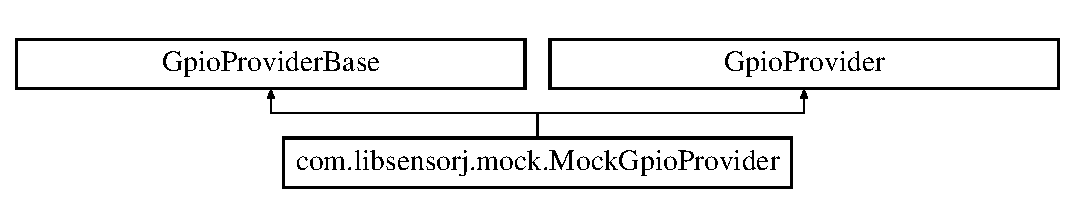
\includegraphics[height=2.000000cm]{classcom_1_1libsensorj_1_1mock_1_1MockGpioProvider}
\end{center}
\end{figure}
\subsection*{Public Member Functions}
\begin{DoxyCompactItemize}
\item 
String \hyperlink{classcom_1_1libsensorj_1_1mock_1_1MockGpioProvider_a85baa28148a2bc5d86eb3c125cf9ab95}{get\+Name} ()
\item 
void \hyperlink{classcom_1_1libsensorj_1_1mock_1_1MockGpioProvider_a944ae745f738b724735611f83016ea7e}{set\+Mock\+State} (Pin pin, Pin\+State state)
\item 
void \hyperlink{classcom_1_1libsensorj_1_1mock_1_1MockGpioProvider_a973c113dff5f3a22241911b0bd9da82e}{set\+Mock\+Analog\+Value} (Pin pin, double value)
\end{DoxyCompactItemize}
\subsection*{Static Public Attributes}
\begin{DoxyCompactItemize}
\item 
static final String \hyperlink{classcom_1_1libsensorj_1_1mock_1_1MockGpioProvider_a55a768da1d26ad878cb1bb2c55de8b0c}{N\+A\+M\+E} = \char`\"{}Mock\+Gpio\+Provider\char`\"{}
\end{DoxyCompactItemize}


\subsection{Detailed Description}
The Class \hyperlink{classcom_1_1libsensorj_1_1mock_1_1MockGpioProvider}{Mock\+Gpio\+Provider}. 

\subsection{Member Function Documentation}
\hypertarget{classcom_1_1libsensorj_1_1mock_1_1MockGpioProvider_a85baa28148a2bc5d86eb3c125cf9ab95}{}\index{com\+::libsensorj\+::mock\+::\+Mock\+Gpio\+Provider@{com\+::libsensorj\+::mock\+::\+Mock\+Gpio\+Provider}!get\+Name@{get\+Name}}
\index{get\+Name@{get\+Name}!com\+::libsensorj\+::mock\+::\+Mock\+Gpio\+Provider@{com\+::libsensorj\+::mock\+::\+Mock\+Gpio\+Provider}}
\subsubsection[{get\+Name}]{\setlength{\rightskip}{0pt plus 5cm}String com.\+libsensorj.\+mock.\+Mock\+Gpio\+Provider.\+get\+Name (
\begin{DoxyParamCaption}
{}
\end{DoxyParamCaption}
)}\label{classcom_1_1libsensorj_1_1mock_1_1MockGpioProvider_a85baa28148a2bc5d86eb3c125cf9ab95}
\hypertarget{classcom_1_1libsensorj_1_1mock_1_1MockGpioProvider_a973c113dff5f3a22241911b0bd9da82e}{}\index{com\+::libsensorj\+::mock\+::\+Mock\+Gpio\+Provider@{com\+::libsensorj\+::mock\+::\+Mock\+Gpio\+Provider}!set\+Mock\+Analog\+Value@{set\+Mock\+Analog\+Value}}
\index{set\+Mock\+Analog\+Value@{set\+Mock\+Analog\+Value}!com\+::libsensorj\+::mock\+::\+Mock\+Gpio\+Provider@{com\+::libsensorj\+::mock\+::\+Mock\+Gpio\+Provider}}
\subsubsection[{set\+Mock\+Analog\+Value}]{\setlength{\rightskip}{0pt plus 5cm}void com.\+libsensorj.\+mock.\+Mock\+Gpio\+Provider.\+set\+Mock\+Analog\+Value (
\begin{DoxyParamCaption}
\item[{Pin}]{pin, }
\item[{double}]{value}
\end{DoxyParamCaption}
)}\label{classcom_1_1libsensorj_1_1mock_1_1MockGpioProvider_a973c113dff5f3a22241911b0bd9da82e}
Sets the mock analog value.


\begin{DoxyParams}{Parameters}
{\em pin} & the pin \\
\hline
{\em value} & the value \\
\hline
\end{DoxyParams}
\hypertarget{classcom_1_1libsensorj_1_1mock_1_1MockGpioProvider_a944ae745f738b724735611f83016ea7e}{}\index{com\+::libsensorj\+::mock\+::\+Mock\+Gpio\+Provider@{com\+::libsensorj\+::mock\+::\+Mock\+Gpio\+Provider}!set\+Mock\+State@{set\+Mock\+State}}
\index{set\+Mock\+State@{set\+Mock\+State}!com\+::libsensorj\+::mock\+::\+Mock\+Gpio\+Provider@{com\+::libsensorj\+::mock\+::\+Mock\+Gpio\+Provider}}
\subsubsection[{set\+Mock\+State}]{\setlength{\rightskip}{0pt plus 5cm}void com.\+libsensorj.\+mock.\+Mock\+Gpio\+Provider.\+set\+Mock\+State (
\begin{DoxyParamCaption}
\item[{Pin}]{pin, }
\item[{Pin\+State}]{state}
\end{DoxyParamCaption}
)}\label{classcom_1_1libsensorj_1_1mock_1_1MockGpioProvider_a944ae745f738b724735611f83016ea7e}
Sets the mock state.


\begin{DoxyParams}{Parameters}
{\em pin} & the pin \\
\hline
{\em state} & the state \\
\hline
\end{DoxyParams}


\subsection{Member Data Documentation}
\hypertarget{classcom_1_1libsensorj_1_1mock_1_1MockGpioProvider_a55a768da1d26ad878cb1bb2c55de8b0c}{}\index{com\+::libsensorj\+::mock\+::\+Mock\+Gpio\+Provider@{com\+::libsensorj\+::mock\+::\+Mock\+Gpio\+Provider}!N\+A\+M\+E@{N\+A\+M\+E}}
\index{N\+A\+M\+E@{N\+A\+M\+E}!com\+::libsensorj\+::mock\+::\+Mock\+Gpio\+Provider@{com\+::libsensorj\+::mock\+::\+Mock\+Gpio\+Provider}}
\subsubsection[{N\+A\+M\+E}]{\setlength{\rightskip}{0pt plus 5cm}final String com.\+libsensorj.\+mock.\+Mock\+Gpio\+Provider.\+N\+A\+M\+E = \char`\"{}Mock\+Gpio\+Provider\char`\"{}\hspace{0.3cm}{\ttfamily [static]}}\label{classcom_1_1libsensorj_1_1mock_1_1MockGpioProvider_a55a768da1d26ad878cb1bb2c55de8b0c}
The Constant N\+A\+M\+E. 

The documentation for this class was generated from the following file\+:\begin{DoxyCompactItemize}
\item 
test/java/com/libsensorj/mock/\hyperlink{MockGpioProvider_8java}{Mock\+Gpio\+Provider.\+java}\end{DoxyCompactItemize}

\hypertarget{classcom_1_1libsensorj_1_1mock_1_1MockPin}{}\section{com.\+libsensorj.\+mock.\+Mock\+Pin Class Reference}
\label{classcom_1_1libsensorj_1_1mock_1_1MockPin}\index{com.\+libsensorj.\+mock.\+Mock\+Pin@{com.\+libsensorj.\+mock.\+Mock\+Pin}}
\subsection*{Static Public Attributes}
\begin{DoxyCompactItemize}
\item 
static final Pin \hyperlink{classcom_1_1libsensorj_1_1mock_1_1MockPin_a4dc35775be540ac9c62c2797c08a7ed7}{D\+I\+G\+I\+T\+A\+L\+\_\+\+B\+I\+D\+I\+R\+E\+C\+T\+I\+O\+N\+A\+L\+\_\+\+P\+I\+N}
\item 
static final Pin \hyperlink{classcom_1_1libsensorj_1_1mock_1_1MockPin_ab3330359048ec50eec255e0ab6309f48}{D\+I\+G\+I\+T\+A\+L\+\_\+\+I\+N\+P\+U\+T\+\_\+\+P\+I\+N}
\item 
static final Pin \hyperlink{classcom_1_1libsensorj_1_1mock_1_1MockPin_ae16d327cdbddbbdeb9314b6b28a52e82}{D\+I\+G\+I\+T\+A\+L\+\_\+\+O\+U\+T\+P\+U\+T\+\_\+\+P\+I\+N}
\item 
static final Pin \hyperlink{classcom_1_1libsensorj_1_1mock_1_1MockPin_af15fcc7a04ad7751ca96f968d1ac1b91}{P\+W\+M\+\_\+\+O\+U\+T\+P\+U\+T\+\_\+\+P\+I\+N}
\item 
static final Pin \hyperlink{classcom_1_1libsensorj_1_1mock_1_1MockPin_a09976649e41290f5aa6c0d61fee67eda}{A\+N\+A\+L\+O\+G\+\_\+\+B\+I\+D\+I\+R\+E\+C\+T\+I\+O\+N\+A\+L\+\_\+\+P\+I\+N}
\item 
static final Pin \hyperlink{classcom_1_1libsensorj_1_1mock_1_1MockPin_a3ca873ea424dac948fabb4c2249ea0a3}{A\+N\+A\+L\+O\+G\+\_\+\+I\+N\+P\+U\+T\+\_\+\+P\+I\+N}
\item 
static final Pin \hyperlink{classcom_1_1libsensorj_1_1mock_1_1MockPin_ac0cb98f53fad4d229f1999253428e252}{A\+N\+A\+L\+O\+G\+\_\+\+O\+U\+T\+P\+U\+T\+\_\+\+P\+I\+N}
\end{DoxyCompactItemize}


\subsection{Detailed Description}
The Class \hyperlink{classcom_1_1libsensorj_1_1mock_1_1MockPin}{Mock\+Pin}. 

\subsection{Member Data Documentation}
\hypertarget{classcom_1_1libsensorj_1_1mock_1_1MockPin_a09976649e41290f5aa6c0d61fee67eda}{}\index{com\+::libsensorj\+::mock\+::\+Mock\+Pin@{com\+::libsensorj\+::mock\+::\+Mock\+Pin}!A\+N\+A\+L\+O\+G\+\_\+\+B\+I\+D\+I\+R\+E\+C\+T\+I\+O\+N\+A\+L\+\_\+\+P\+I\+N@{A\+N\+A\+L\+O\+G\+\_\+\+B\+I\+D\+I\+R\+E\+C\+T\+I\+O\+N\+A\+L\+\_\+\+P\+I\+N}}
\index{A\+N\+A\+L\+O\+G\+\_\+\+B\+I\+D\+I\+R\+E\+C\+T\+I\+O\+N\+A\+L\+\_\+\+P\+I\+N@{A\+N\+A\+L\+O\+G\+\_\+\+B\+I\+D\+I\+R\+E\+C\+T\+I\+O\+N\+A\+L\+\_\+\+P\+I\+N}!com\+::libsensorj\+::mock\+::\+Mock\+Pin@{com\+::libsensorj\+::mock\+::\+Mock\+Pin}}
\subsubsection[{A\+N\+A\+L\+O\+G\+\_\+\+B\+I\+D\+I\+R\+E\+C\+T\+I\+O\+N\+A\+L\+\_\+\+P\+I\+N}]{\setlength{\rightskip}{0pt plus 5cm}final Pin com.\+libsensorj.\+mock.\+Mock\+Pin.\+A\+N\+A\+L\+O\+G\+\_\+\+B\+I\+D\+I\+R\+E\+C\+T\+I\+O\+N\+A\+L\+\_\+\+P\+I\+N\hspace{0.3cm}{\ttfamily [static]}}\label{classcom_1_1libsensorj_1_1mock_1_1MockPin_a09976649e41290f5aa6c0d61fee67eda}
{\bfseries Initial value\+:}
\begin{DoxyCode}
= \textcolor{keyword}{new} PinImpl(
            MockGpioProvider.NAME, 4, \textcolor{stringliteral}{"GPIO-4"}, EnumSet.of(
                    PinMode.ANALOG\_INPUT, PinMode.ANALOG\_OUTPUT))
\end{DoxyCode}
The Constant A\+N\+A\+L\+O\+G\+\_\+\+B\+I\+D\+I\+R\+E\+C\+T\+I\+O\+N\+A\+L\+\_\+\+P\+I\+N. \hypertarget{classcom_1_1libsensorj_1_1mock_1_1MockPin_a3ca873ea424dac948fabb4c2249ea0a3}{}\index{com\+::libsensorj\+::mock\+::\+Mock\+Pin@{com\+::libsensorj\+::mock\+::\+Mock\+Pin}!A\+N\+A\+L\+O\+G\+\_\+\+I\+N\+P\+U\+T\+\_\+\+P\+I\+N@{A\+N\+A\+L\+O\+G\+\_\+\+I\+N\+P\+U\+T\+\_\+\+P\+I\+N}}
\index{A\+N\+A\+L\+O\+G\+\_\+\+I\+N\+P\+U\+T\+\_\+\+P\+I\+N@{A\+N\+A\+L\+O\+G\+\_\+\+I\+N\+P\+U\+T\+\_\+\+P\+I\+N}!com\+::libsensorj\+::mock\+::\+Mock\+Pin@{com\+::libsensorj\+::mock\+::\+Mock\+Pin}}
\subsubsection[{A\+N\+A\+L\+O\+G\+\_\+\+I\+N\+P\+U\+T\+\_\+\+P\+I\+N}]{\setlength{\rightskip}{0pt plus 5cm}final Pin com.\+libsensorj.\+mock.\+Mock\+Pin.\+A\+N\+A\+L\+O\+G\+\_\+\+I\+N\+P\+U\+T\+\_\+\+P\+I\+N\hspace{0.3cm}{\ttfamily [static]}}\label{classcom_1_1libsensorj_1_1mock_1_1MockPin_a3ca873ea424dac948fabb4c2249ea0a3}
{\bfseries Initial value\+:}
\begin{DoxyCode}
= \textcolor{keyword}{new} PinImpl(
            MockGpioProvider.NAME, 5, \textcolor{stringliteral}{"GPIO-5"},
            EnumSet.of(PinMode.ANALOG\_INPUT))
\end{DoxyCode}
The Constant A\+N\+A\+L\+O\+G\+\_\+\+I\+N\+P\+U\+T\+\_\+\+P\+I\+N. \hypertarget{classcom_1_1libsensorj_1_1mock_1_1MockPin_ac0cb98f53fad4d229f1999253428e252}{}\index{com\+::libsensorj\+::mock\+::\+Mock\+Pin@{com\+::libsensorj\+::mock\+::\+Mock\+Pin}!A\+N\+A\+L\+O\+G\+\_\+\+O\+U\+T\+P\+U\+T\+\_\+\+P\+I\+N@{A\+N\+A\+L\+O\+G\+\_\+\+O\+U\+T\+P\+U\+T\+\_\+\+P\+I\+N}}
\index{A\+N\+A\+L\+O\+G\+\_\+\+O\+U\+T\+P\+U\+T\+\_\+\+P\+I\+N@{A\+N\+A\+L\+O\+G\+\_\+\+O\+U\+T\+P\+U\+T\+\_\+\+P\+I\+N}!com\+::libsensorj\+::mock\+::\+Mock\+Pin@{com\+::libsensorj\+::mock\+::\+Mock\+Pin}}
\subsubsection[{A\+N\+A\+L\+O\+G\+\_\+\+O\+U\+T\+P\+U\+T\+\_\+\+P\+I\+N}]{\setlength{\rightskip}{0pt plus 5cm}final Pin com.\+libsensorj.\+mock.\+Mock\+Pin.\+A\+N\+A\+L\+O\+G\+\_\+\+O\+U\+T\+P\+U\+T\+\_\+\+P\+I\+N\hspace{0.3cm}{\ttfamily [static]}}\label{classcom_1_1libsensorj_1_1mock_1_1MockPin_ac0cb98f53fad4d229f1999253428e252}
{\bfseries Initial value\+:}
\begin{DoxyCode}
= \textcolor{keyword}{new} PinImpl(
            MockGpioProvider.NAME, 6, \textcolor{stringliteral}{"GPIO-6"},
            EnumSet.of(PinMode.ANALOG\_OUTPUT))
\end{DoxyCode}
The Constant A\+N\+A\+L\+O\+G\+\_\+\+O\+U\+T\+P\+U\+T\+\_\+\+P\+I\+N. \hypertarget{classcom_1_1libsensorj_1_1mock_1_1MockPin_a4dc35775be540ac9c62c2797c08a7ed7}{}\index{com\+::libsensorj\+::mock\+::\+Mock\+Pin@{com\+::libsensorj\+::mock\+::\+Mock\+Pin}!D\+I\+G\+I\+T\+A\+L\+\_\+\+B\+I\+D\+I\+R\+E\+C\+T\+I\+O\+N\+A\+L\+\_\+\+P\+I\+N@{D\+I\+G\+I\+T\+A\+L\+\_\+\+B\+I\+D\+I\+R\+E\+C\+T\+I\+O\+N\+A\+L\+\_\+\+P\+I\+N}}
\index{D\+I\+G\+I\+T\+A\+L\+\_\+\+B\+I\+D\+I\+R\+E\+C\+T\+I\+O\+N\+A\+L\+\_\+\+P\+I\+N@{D\+I\+G\+I\+T\+A\+L\+\_\+\+B\+I\+D\+I\+R\+E\+C\+T\+I\+O\+N\+A\+L\+\_\+\+P\+I\+N}!com\+::libsensorj\+::mock\+::\+Mock\+Pin@{com\+::libsensorj\+::mock\+::\+Mock\+Pin}}
\subsubsection[{D\+I\+G\+I\+T\+A\+L\+\_\+\+B\+I\+D\+I\+R\+E\+C\+T\+I\+O\+N\+A\+L\+\_\+\+P\+I\+N}]{\setlength{\rightskip}{0pt plus 5cm}final Pin com.\+libsensorj.\+mock.\+Mock\+Pin.\+D\+I\+G\+I\+T\+A\+L\+\_\+\+B\+I\+D\+I\+R\+E\+C\+T\+I\+O\+N\+A\+L\+\_\+\+P\+I\+N\hspace{0.3cm}{\ttfamily [static]}}\label{classcom_1_1libsensorj_1_1mock_1_1MockPin_a4dc35775be540ac9c62c2797c08a7ed7}
{\bfseries Initial value\+:}
\begin{DoxyCode}
= \textcolor{keyword}{new} PinImpl(
            MockGpioProvider.NAME, 0, \textcolor{stringliteral}{"GPIO-0"}, EnumSet.of(
                    PinMode.DIGITAL\_INPUT, PinMode.DIGITAL\_OUTPUT),
            PinPullResistance.all())
\end{DoxyCode}
The Constant D\+I\+G\+I\+T\+A\+L\+\_\+\+B\+I\+D\+I\+R\+E\+C\+T\+I\+O\+N\+A\+L\+\_\+\+P\+I\+N. \hypertarget{classcom_1_1libsensorj_1_1mock_1_1MockPin_ab3330359048ec50eec255e0ab6309f48}{}\index{com\+::libsensorj\+::mock\+::\+Mock\+Pin@{com\+::libsensorj\+::mock\+::\+Mock\+Pin}!D\+I\+G\+I\+T\+A\+L\+\_\+\+I\+N\+P\+U\+T\+\_\+\+P\+I\+N@{D\+I\+G\+I\+T\+A\+L\+\_\+\+I\+N\+P\+U\+T\+\_\+\+P\+I\+N}}
\index{D\+I\+G\+I\+T\+A\+L\+\_\+\+I\+N\+P\+U\+T\+\_\+\+P\+I\+N@{D\+I\+G\+I\+T\+A\+L\+\_\+\+I\+N\+P\+U\+T\+\_\+\+P\+I\+N}!com\+::libsensorj\+::mock\+::\+Mock\+Pin@{com\+::libsensorj\+::mock\+::\+Mock\+Pin}}
\subsubsection[{D\+I\+G\+I\+T\+A\+L\+\_\+\+I\+N\+P\+U\+T\+\_\+\+P\+I\+N}]{\setlength{\rightskip}{0pt plus 5cm}final Pin com.\+libsensorj.\+mock.\+Mock\+Pin.\+D\+I\+G\+I\+T\+A\+L\+\_\+\+I\+N\+P\+U\+T\+\_\+\+P\+I\+N\hspace{0.3cm}{\ttfamily [static]}}\label{classcom_1_1libsensorj_1_1mock_1_1MockPin_ab3330359048ec50eec255e0ab6309f48}
{\bfseries Initial value\+:}
\begin{DoxyCode}
= \textcolor{keyword}{new} PinImpl(
            MockGpioProvider.NAME, 1, \textcolor{stringliteral}{"GPIO-1"},
            EnumSet.of(PinMode.DIGITAL\_INPUT), PinPullResistance.all())
\end{DoxyCode}
The Constant D\+I\+G\+I\+T\+A\+L\+\_\+\+I\+N\+P\+U\+T\+\_\+\+P\+I\+N. \hypertarget{classcom_1_1libsensorj_1_1mock_1_1MockPin_ae16d327cdbddbbdeb9314b6b28a52e82}{}\index{com\+::libsensorj\+::mock\+::\+Mock\+Pin@{com\+::libsensorj\+::mock\+::\+Mock\+Pin}!D\+I\+G\+I\+T\+A\+L\+\_\+\+O\+U\+T\+P\+U\+T\+\_\+\+P\+I\+N@{D\+I\+G\+I\+T\+A\+L\+\_\+\+O\+U\+T\+P\+U\+T\+\_\+\+P\+I\+N}}
\index{D\+I\+G\+I\+T\+A\+L\+\_\+\+O\+U\+T\+P\+U\+T\+\_\+\+P\+I\+N@{D\+I\+G\+I\+T\+A\+L\+\_\+\+O\+U\+T\+P\+U\+T\+\_\+\+P\+I\+N}!com\+::libsensorj\+::mock\+::\+Mock\+Pin@{com\+::libsensorj\+::mock\+::\+Mock\+Pin}}
\subsubsection[{D\+I\+G\+I\+T\+A\+L\+\_\+\+O\+U\+T\+P\+U\+T\+\_\+\+P\+I\+N}]{\setlength{\rightskip}{0pt plus 5cm}final Pin com.\+libsensorj.\+mock.\+Mock\+Pin.\+D\+I\+G\+I\+T\+A\+L\+\_\+\+O\+U\+T\+P\+U\+T\+\_\+\+P\+I\+N\hspace{0.3cm}{\ttfamily [static]}}\label{classcom_1_1libsensorj_1_1mock_1_1MockPin_ae16d327cdbddbbdeb9314b6b28a52e82}
{\bfseries Initial value\+:}
\begin{DoxyCode}
= \textcolor{keyword}{new} PinImpl(
            MockGpioProvider.NAME, 2, \textcolor{stringliteral}{"GPIO-2"},
            EnumSet.of(PinMode.DIGITAL\_OUTPUT))
\end{DoxyCode}
The Constant D\+I\+G\+I\+T\+A\+L\+\_\+\+O\+U\+T\+P\+U\+T\+\_\+\+P\+I\+N. \hypertarget{classcom_1_1libsensorj_1_1mock_1_1MockPin_af15fcc7a04ad7751ca96f968d1ac1b91}{}\index{com\+::libsensorj\+::mock\+::\+Mock\+Pin@{com\+::libsensorj\+::mock\+::\+Mock\+Pin}!P\+W\+M\+\_\+\+O\+U\+T\+P\+U\+T\+\_\+\+P\+I\+N@{P\+W\+M\+\_\+\+O\+U\+T\+P\+U\+T\+\_\+\+P\+I\+N}}
\index{P\+W\+M\+\_\+\+O\+U\+T\+P\+U\+T\+\_\+\+P\+I\+N@{P\+W\+M\+\_\+\+O\+U\+T\+P\+U\+T\+\_\+\+P\+I\+N}!com\+::libsensorj\+::mock\+::\+Mock\+Pin@{com\+::libsensorj\+::mock\+::\+Mock\+Pin}}
\subsubsection[{P\+W\+M\+\_\+\+O\+U\+T\+P\+U\+T\+\_\+\+P\+I\+N}]{\setlength{\rightskip}{0pt plus 5cm}final Pin com.\+libsensorj.\+mock.\+Mock\+Pin.\+P\+W\+M\+\_\+\+O\+U\+T\+P\+U\+T\+\_\+\+P\+I\+N\hspace{0.3cm}{\ttfamily [static]}}\label{classcom_1_1libsensorj_1_1mock_1_1MockPin_af15fcc7a04ad7751ca96f968d1ac1b91}
{\bfseries Initial value\+:}
\begin{DoxyCode}
= \textcolor{keyword}{new} PinImpl(MockGpioProvider.NAME,
            3, \textcolor{stringliteral}{"GPIO-3"}, EnumSet.of(PinMode.PWM\_OUTPUT))
\end{DoxyCode}
The Constant P\+W\+M\+\_\+\+O\+U\+T\+P\+U\+T\+\_\+\+P\+I\+N. 

The documentation for this class was generated from the following file\+:\begin{DoxyCompactItemize}
\item 
test/java/com/libsensorj/mock/\hyperlink{MockPin_8java}{Mock\+Pin.\+java}\end{DoxyCompactItemize}

\hypertarget{classcom_1_1pi4j_1_1examples_1_1MyExample}{}\section{com.\+pi4j.\+examples.\+My\+Example Class Reference}
\label{classcom_1_1pi4j_1_1examples_1_1MyExample}\index{com.\+pi4j.\+examples.\+My\+Example@{com.\+pi4j.\+examples.\+My\+Example}}
\subsection*{Static Public Member Functions}
\begin{DoxyCompactItemize}
\item 
static void \hyperlink{classcom_1_1pi4j_1_1examples_1_1MyExample_a535756901ce4a1b547faf38117a3ec6f}{main} (String\mbox{[}$\,$\mbox{]} args)
\end{DoxyCompactItemize}


\subsection{Detailed Description}
The Class \hyperlink{classcom_1_1pi4j_1_1examples_1_1MyExample}{My\+Example}. 

\subsection{Member Function Documentation}
\hypertarget{classcom_1_1pi4j_1_1examples_1_1MyExample_a535756901ce4a1b547faf38117a3ec6f}{}\index{com\+::pi4j\+::examples\+::\+My\+Example@{com\+::pi4j\+::examples\+::\+My\+Example}!main@{main}}
\index{main@{main}!com\+::pi4j\+::examples\+::\+My\+Example@{com\+::pi4j\+::examples\+::\+My\+Example}}
\subsubsection[{main}]{\setlength{\rightskip}{0pt plus 5cm}static void com.\+pi4j.\+examples.\+My\+Example.\+main (
\begin{DoxyParamCaption}
\item[{String\mbox{[}$\,$\mbox{]}}]{args}
\end{DoxyParamCaption}
)\hspace{0.3cm}{\ttfamily [static]}}\label{classcom_1_1pi4j_1_1examples_1_1MyExample_a535756901ce4a1b547faf38117a3ec6f}
The main method.


\begin{DoxyParams}{Parameters}
{\em args} & the arguments \\
\hline
\end{DoxyParams}


The documentation for this class was generated from the following file\+:\begin{DoxyCompactItemize}
\item 
main/java/com/pi4j/examples/\hyperlink{MyExample_8java}{My\+Example.\+java}\end{DoxyCompactItemize}

\hypertarget{classcom_1_1libsensorj_1_1model_1_1Observer}{}\section{com.\+libsensorj.\+model.\+Observer Class Reference}
\label{classcom_1_1libsensorj_1_1model_1_1Observer}\index{com.\+libsensorj.\+model.\+Observer@{com.\+libsensorj.\+model.\+Observer}}
\subsection*{Public Member Functions}
\begin{DoxyCompactItemize}
\item 
\hyperlink{classcom_1_1libsensorj_1_1model_1_1Observer_a477725e32a58d3a8762d404799ec0161}{Observer} ()
\item 
\hyperlink{classcom_1_1libsensorj_1_1model_1_1Observer_a4933adee4c8da771eaa94415f6f840a7}{Observer} (String \hyperlink{classcom_1_1libsensorj_1_1model_1_1Observer_aa1f9da7634c35f34d5f20d5bc1562428}{observer\+Name})
\item 
String \hyperlink{classcom_1_1libsensorj_1_1model_1_1Observer_a8b873b9c90ad7f1ed055ea6713e0062a}{get\+Observer\+Name} ()
\item 
void \hyperlink{classcom_1_1libsensorj_1_1model_1_1Observer_a42628ca2b4d99e0df9fe1d70fec811b2}{set\+Observer\+Name} (String \hyperlink{classcom_1_1libsensorj_1_1model_1_1Observer_aa1f9da7634c35f34d5f20d5bc1562428}{observer\+Name})
\end{DoxyCompactItemize}
\subsection*{Private Attributes}
\begin{DoxyCompactItemize}
\item 
String \hyperlink{classcom_1_1libsensorj_1_1model_1_1Observer_aa1f9da7634c35f34d5f20d5bc1562428}{observer\+Name}
\end{DoxyCompactItemize}


\subsection{Detailed Description}
The Class \hyperlink{classcom_1_1libsensorj_1_1model_1_1Observer}{Observer}. 

\subsection{Constructor \& Destructor Documentation}
\hypertarget{classcom_1_1libsensorj_1_1model_1_1Observer_a477725e32a58d3a8762d404799ec0161}{}\index{com\+::libsensorj\+::model\+::\+Observer@{com\+::libsensorj\+::model\+::\+Observer}!Observer@{Observer}}
\index{Observer@{Observer}!com\+::libsensorj\+::model\+::\+Observer@{com\+::libsensorj\+::model\+::\+Observer}}
\subsubsection[{Observer}]{\setlength{\rightskip}{0pt plus 5cm}com.\+libsensorj.\+model.\+Observer.\+Observer (
\begin{DoxyParamCaption}
{}
\end{DoxyParamCaption}
)}\label{classcom_1_1libsensorj_1_1model_1_1Observer_a477725e32a58d3a8762d404799ec0161}
Instantiates a new observer. \hypertarget{classcom_1_1libsensorj_1_1model_1_1Observer_a4933adee4c8da771eaa94415f6f840a7}{}\index{com\+::libsensorj\+::model\+::\+Observer@{com\+::libsensorj\+::model\+::\+Observer}!Observer@{Observer}}
\index{Observer@{Observer}!com\+::libsensorj\+::model\+::\+Observer@{com\+::libsensorj\+::model\+::\+Observer}}
\subsubsection[{Observer}]{\setlength{\rightskip}{0pt plus 5cm}com.\+libsensorj.\+model.\+Observer.\+Observer (
\begin{DoxyParamCaption}
\item[{String}]{observer\+Name}
\end{DoxyParamCaption}
)}\label{classcom_1_1libsensorj_1_1model_1_1Observer_a4933adee4c8da771eaa94415f6f840a7}
Instantiates a new observer.


\begin{DoxyParams}{Parameters}
{\em observer\+Name} & the observer name \\
\hline
\end{DoxyParams}


\subsection{Member Function Documentation}
\hypertarget{classcom_1_1libsensorj_1_1model_1_1Observer_a8b873b9c90ad7f1ed055ea6713e0062a}{}\index{com\+::libsensorj\+::model\+::\+Observer@{com\+::libsensorj\+::model\+::\+Observer}!get\+Observer\+Name@{get\+Observer\+Name}}
\index{get\+Observer\+Name@{get\+Observer\+Name}!com\+::libsensorj\+::model\+::\+Observer@{com\+::libsensorj\+::model\+::\+Observer}}
\subsubsection[{get\+Observer\+Name}]{\setlength{\rightskip}{0pt plus 5cm}String com.\+libsensorj.\+model.\+Observer.\+get\+Observer\+Name (
\begin{DoxyParamCaption}
{}
\end{DoxyParamCaption}
)}\label{classcom_1_1libsensorj_1_1model_1_1Observer_a8b873b9c90ad7f1ed055ea6713e0062a}
Gets the observer name.

\begin{DoxyReturn}{Returns}
the observer name 
\end{DoxyReturn}
\hypertarget{classcom_1_1libsensorj_1_1model_1_1Observer_a42628ca2b4d99e0df9fe1d70fec811b2}{}\index{com\+::libsensorj\+::model\+::\+Observer@{com\+::libsensorj\+::model\+::\+Observer}!set\+Observer\+Name@{set\+Observer\+Name}}
\index{set\+Observer\+Name@{set\+Observer\+Name}!com\+::libsensorj\+::model\+::\+Observer@{com\+::libsensorj\+::model\+::\+Observer}}
\subsubsection[{set\+Observer\+Name}]{\setlength{\rightskip}{0pt plus 5cm}void com.\+libsensorj.\+model.\+Observer.\+set\+Observer\+Name (
\begin{DoxyParamCaption}
\item[{String}]{observer\+Name}
\end{DoxyParamCaption}
)}\label{classcom_1_1libsensorj_1_1model_1_1Observer_a42628ca2b4d99e0df9fe1d70fec811b2}
Sets the observer name.


\begin{DoxyParams}{Parameters}
{\em observer\+Name} & the new observer name \\
\hline
\end{DoxyParams}


\subsection{Member Data Documentation}
\hypertarget{classcom_1_1libsensorj_1_1model_1_1Observer_aa1f9da7634c35f34d5f20d5bc1562428}{}\index{com\+::libsensorj\+::model\+::\+Observer@{com\+::libsensorj\+::model\+::\+Observer}!observer\+Name@{observer\+Name}}
\index{observer\+Name@{observer\+Name}!com\+::libsensorj\+::model\+::\+Observer@{com\+::libsensorj\+::model\+::\+Observer}}
\subsubsection[{observer\+Name}]{\setlength{\rightskip}{0pt plus 5cm}String com.\+libsensorj.\+model.\+Observer.\+observer\+Name\hspace{0.3cm}{\ttfamily [private]}}\label{classcom_1_1libsensorj_1_1model_1_1Observer_aa1f9da7634c35f34d5f20d5bc1562428}
The observer name. 

The documentation for this class was generated from the following file\+:\begin{DoxyCompactItemize}
\item 
main/java/com/libsensorj/model/\hyperlink{Observer_8java}{Observer.\+java}\end{DoxyCompactItemize}

\hypertarget{enumcom_1_1libsensorj_1_1utils_1_1PinNumbers}{}\section{com.\+libsensorj.\+utils.\+Pin\+Numbers Enum Reference}
\label{enumcom_1_1libsensorj_1_1utils_1_1PinNumbers}\index{com.\+libsensorj.\+utils.\+Pin\+Numbers@{com.\+libsensorj.\+utils.\+Pin\+Numbers}}
\subsection*{Public Member Functions}
\begin{DoxyCompactItemize}
\item 
\hyperlink{enumcom_1_1libsensorj_1_1utils_1_1PinNumbers_a968a61df9cb0d58d376afe58c0e819a1}{Pin\+Numbers} (Pin pin)
\end{DoxyCompactItemize}
\subsection*{Public Attributes}
\begin{DoxyCompactItemize}
\item 
\hyperlink{enumcom_1_1libsensorj_1_1utils_1_1PinNumbers_a3ef0e0eade17450513e7722a45850223}{P\+I\+N\+\_\+00} =(Raspi\+Pin.\+G\+P\+I\+O\+\_\+00)
\item 
\hyperlink{enumcom_1_1libsensorj_1_1utils_1_1PinNumbers_a685c54b4b889232a644256053628b751}{P\+I\+N\+\_\+01} =(Raspi\+Pin.\+G\+P\+I\+O\+\_\+01)
\item 
\hyperlink{enumcom_1_1libsensorj_1_1utils_1_1PinNumbers_afb610737394f458dff87b1df785b75ea}{P\+I\+N\+\_\+02} =(Raspi\+Pin.\+G\+P\+I\+O\+\_\+02)
\item 
\hyperlink{enumcom_1_1libsensorj_1_1utils_1_1PinNumbers_a1bc2b6b45afefca090b810e9f8acbb27}{P\+I\+N\+\_\+03} =(Raspi\+Pin.\+G\+P\+I\+O\+\_\+03)
\item 
\hyperlink{enumcom_1_1libsensorj_1_1utils_1_1PinNumbers_a93afd56e9549da0c1d58a541be66bd3e}{P\+I\+N\+\_\+04} =(Raspi\+Pin.\+G\+P\+I\+O\+\_\+04)
\item 
\hyperlink{enumcom_1_1libsensorj_1_1utils_1_1PinNumbers_ae8da4fe40f2c19e201f9bfc201144c5a}{P\+I\+N\+\_\+05} =(Raspi\+Pin.\+G\+P\+I\+O\+\_\+05)
\item 
\hyperlink{enumcom_1_1libsensorj_1_1utils_1_1PinNumbers_a04c882940fbe6fa70f06f533f0693e5d}{P\+I\+N\+\_\+06} =(Raspi\+Pin.\+G\+P\+I\+O\+\_\+06)
\item 
\hyperlink{enumcom_1_1libsensorj_1_1utils_1_1PinNumbers_ab8b7352afed72c8b1ea2c55d9050b99b}{P\+I\+N\+\_\+07} =(Raspi\+Pin.\+G\+P\+I\+O\+\_\+07)
\item 
\hyperlink{enumcom_1_1libsensorj_1_1utils_1_1PinNumbers_a9d3ead7c0ee9cc96ab2b4f2519c3e4e4}{P\+I\+N\+\_\+08} =(Raspi\+Pin.\+G\+P\+I\+O\+\_\+08)
\item 
\hyperlink{enumcom_1_1libsensorj_1_1utils_1_1PinNumbers_a054eb5753d44984377ca36b6bd790543}{P\+I\+N\+\_\+09} =(Raspi\+Pin.\+G\+P\+I\+O\+\_\+09)
\item 
\hyperlink{enumcom_1_1libsensorj_1_1utils_1_1PinNumbers_a239afb6f67b7e2515ba8cba38c139f25}{P\+I\+N\+\_\+10} =(Raspi\+Pin.\+G\+P\+I\+O\+\_\+10)
\item 
\hyperlink{enumcom_1_1libsensorj_1_1utils_1_1PinNumbers_a5ee3dd0f90eb66a8594ad89a2a0470eb}{P\+I\+N\+\_\+11} =(Raspi\+Pin.\+G\+P\+I\+O\+\_\+11)
\item 
\hyperlink{enumcom_1_1libsensorj_1_1utils_1_1PinNumbers_ae19026133ddb5e75c9778599fcb803fe}{P\+I\+N\+\_\+12} =(Raspi\+Pin.\+G\+P\+I\+O\+\_\+12)
\item 
\hyperlink{enumcom_1_1libsensorj_1_1utils_1_1PinNumbers_a5e893c4d5093998d44431b35b7b9ba7c}{P\+I\+N\+\_\+13} =(Raspi\+Pin.\+G\+P\+I\+O\+\_\+13)
\item 
\hyperlink{enumcom_1_1libsensorj_1_1utils_1_1PinNumbers_ac1c99a7202d314de7d9f4a772c55a0ca}{P\+I\+N\+\_\+14} =(Raspi\+Pin.\+G\+P\+I\+O\+\_\+14)
\item 
\hyperlink{enumcom_1_1libsensorj_1_1utils_1_1PinNumbers_a1e89f76fc2c08c4929b36ab869e4c879}{P\+I\+N\+\_\+15} =(Raspi\+Pin.\+G\+P\+I\+O\+\_\+15)
\item 
\hyperlink{enumcom_1_1libsensorj_1_1utils_1_1PinNumbers_a1ffacc29c4eda74be0327a9acd772a1a}{P\+I\+N\+\_\+16} =(Raspi\+Pin.\+G\+P\+I\+O\+\_\+16)
\item 
\hyperlink{enumcom_1_1libsensorj_1_1utils_1_1PinNumbers_a6d060a58a23f8f9ab2af2b3787919db5}{P\+I\+N\+\_\+17} =(Raspi\+Pin.\+G\+P\+I\+O\+\_\+17)
\item 
\hyperlink{enumcom_1_1libsensorj_1_1utils_1_1PinNumbers_ac6d1e80afe2e16591fa1de746930670a}{P\+I\+N\+\_\+18} =(Raspi\+Pin.\+G\+P\+I\+O\+\_\+18)
\item 
\hyperlink{enumcom_1_1libsensorj_1_1utils_1_1PinNumbers_a4443c323b9599c9f323734c354bf4b03}{P\+I\+N\+\_\+19} =(Raspi\+Pin.\+G\+P\+I\+O\+\_\+19)
\item 
\hyperlink{enumcom_1_1libsensorj_1_1utils_1_1PinNumbers_a7382cd6abefb7891a990e1e4919923da}{P\+I\+N\+\_\+20} =(Raspi\+Pin.\+G\+P\+I\+O\+\_\+20)
\item 
\hyperlink{enumcom_1_1libsensorj_1_1utils_1_1PinNumbers_a53700cbc79faf1650f0f46862458a524}{P\+I\+N\+\_\+21} =(Raspi\+Pin.\+G\+P\+I\+O\+\_\+21)
\item 
\hyperlink{enumcom_1_1libsensorj_1_1utils_1_1PinNumbers_a136ce66a6474359af2728ac7bf4b81db}{P\+I\+N\+\_\+22} =(Raspi\+Pin.\+G\+P\+I\+O\+\_\+22)
\item 
\hyperlink{enumcom_1_1libsensorj_1_1utils_1_1PinNumbers_a5c12880fb3fca2bfede5782df98de3bb}{P\+I\+N\+\_\+23} =(Raspi\+Pin.\+G\+P\+I\+O\+\_\+23)
\item 
\hyperlink{enumcom_1_1libsensorj_1_1utils_1_1PinNumbers_a8d54d3af55e1b5460f88d7faa218e545}{P\+I\+N\+\_\+24} =(Raspi\+Pin.\+G\+P\+I\+O\+\_\+24)
\item 
\hyperlink{enumcom_1_1libsensorj_1_1utils_1_1PinNumbers_a64907a187e76e03b5071d26b42bc8ff7}{P\+I\+N\+\_\+25} =(Raspi\+Pin.\+G\+P\+I\+O\+\_\+25)
\item 
\hyperlink{enumcom_1_1libsensorj_1_1utils_1_1PinNumbers_a66592f4af694df2ec1605d26f3b9f458}{P\+I\+N\+\_\+26} =(Raspi\+Pin.\+G\+P\+I\+O\+\_\+26)
\item 
\hyperlink{enumcom_1_1libsensorj_1_1utils_1_1PinNumbers_ac5368fe64b7b6003c89065bea9e7ca49}{P\+I\+N\+\_\+27} =(Raspi\+Pin.\+G\+P\+I\+O\+\_\+27)
\item 
\hyperlink{enumcom_1_1libsensorj_1_1utils_1_1PinNumbers_af7bec7611fed7e9b64e25485f2378f81}{P\+I\+N\+\_\+28} =(Raspi\+Pin.\+G\+P\+I\+O\+\_\+28)
\item 
\hyperlink{enumcom_1_1libsensorj_1_1utils_1_1PinNumbers_a78cc24e6c72e7dceb4a9a152cc9da41f}{P\+I\+N\+\_\+29} =(Raspi\+Pin.\+G\+P\+I\+O\+\_\+29)
\item 
Pin \hyperlink{enumcom_1_1libsensorj_1_1utils_1_1PinNumbers_a82cad4bc9bde38b8b6e9f33f5ce8bf3d}{pin\+Number}
\end{DoxyCompactItemize}


\subsection{Detailed Description}
The Enum \hyperlink{enumcom_1_1libsensorj_1_1utils_1_1PinNumbers}{Pin\+Numbers}. 

\subsection{Constructor \& Destructor Documentation}
\hypertarget{enumcom_1_1libsensorj_1_1utils_1_1PinNumbers_a968a61df9cb0d58d376afe58c0e819a1}{}\index{com\+::libsensorj\+::utils\+::\+Pin\+Numbers@{com\+::libsensorj\+::utils\+::\+Pin\+Numbers}!Pin\+Numbers@{Pin\+Numbers}}
\index{Pin\+Numbers@{Pin\+Numbers}!com\+::libsensorj\+::utils\+::\+Pin\+Numbers@{com\+::libsensorj\+::utils\+::\+Pin\+Numbers}}
\subsubsection[{Pin\+Numbers}]{\setlength{\rightskip}{0pt plus 5cm}com.\+libsensorj.\+utils.\+Pin\+Numbers.\+Pin\+Numbers (
\begin{DoxyParamCaption}
\item[{Pin}]{pin}
\end{DoxyParamCaption}
)}\label{enumcom_1_1libsensorj_1_1utils_1_1PinNumbers_a968a61df9cb0d58d376afe58c0e819a1}
Instantiates new pin numbers.


\begin{DoxyParams}{Parameters}
{\em pin} & the pin \\
\hline
\end{DoxyParams}


\subsection{Member Data Documentation}
\hypertarget{enumcom_1_1libsensorj_1_1utils_1_1PinNumbers_a3ef0e0eade17450513e7722a45850223}{}\index{com\+::libsensorj\+::utils\+::\+Pin\+Numbers@{com\+::libsensorj\+::utils\+::\+Pin\+Numbers}!P\+I\+N\+\_\+00@{P\+I\+N\+\_\+00}}
\index{P\+I\+N\+\_\+00@{P\+I\+N\+\_\+00}!com\+::libsensorj\+::utils\+::\+Pin\+Numbers@{com\+::libsensorj\+::utils\+::\+Pin\+Numbers}}
\subsubsection[{P\+I\+N\+\_\+00}]{\setlength{\rightskip}{0pt plus 5cm}com.\+libsensorj.\+utils.\+Pin\+Numbers.\+P\+I\+N\+\_\+00 =(Raspi\+Pin.\+G\+P\+I\+O\+\_\+00)}\label{enumcom_1_1libsensorj_1_1utils_1_1PinNumbers_a3ef0e0eade17450513e7722a45850223}
The P\+I n\+\_\+00. \hypertarget{enumcom_1_1libsensorj_1_1utils_1_1PinNumbers_a685c54b4b889232a644256053628b751}{}\index{com\+::libsensorj\+::utils\+::\+Pin\+Numbers@{com\+::libsensorj\+::utils\+::\+Pin\+Numbers}!P\+I\+N\+\_\+01@{P\+I\+N\+\_\+01}}
\index{P\+I\+N\+\_\+01@{P\+I\+N\+\_\+01}!com\+::libsensorj\+::utils\+::\+Pin\+Numbers@{com\+::libsensorj\+::utils\+::\+Pin\+Numbers}}
\subsubsection[{P\+I\+N\+\_\+01}]{\setlength{\rightskip}{0pt plus 5cm}com.\+libsensorj.\+utils.\+Pin\+Numbers.\+P\+I\+N\+\_\+01 =(Raspi\+Pin.\+G\+P\+I\+O\+\_\+01)}\label{enumcom_1_1libsensorj_1_1utils_1_1PinNumbers_a685c54b4b889232a644256053628b751}
The P\+I n\+\_\+01. \hypertarget{enumcom_1_1libsensorj_1_1utils_1_1PinNumbers_afb610737394f458dff87b1df785b75ea}{}\index{com\+::libsensorj\+::utils\+::\+Pin\+Numbers@{com\+::libsensorj\+::utils\+::\+Pin\+Numbers}!P\+I\+N\+\_\+02@{P\+I\+N\+\_\+02}}
\index{P\+I\+N\+\_\+02@{P\+I\+N\+\_\+02}!com\+::libsensorj\+::utils\+::\+Pin\+Numbers@{com\+::libsensorj\+::utils\+::\+Pin\+Numbers}}
\subsubsection[{P\+I\+N\+\_\+02}]{\setlength{\rightskip}{0pt plus 5cm}com.\+libsensorj.\+utils.\+Pin\+Numbers.\+P\+I\+N\+\_\+02 =(Raspi\+Pin.\+G\+P\+I\+O\+\_\+02)}\label{enumcom_1_1libsensorj_1_1utils_1_1PinNumbers_afb610737394f458dff87b1df785b75ea}
The P\+I n\+\_\+02. \hypertarget{enumcom_1_1libsensorj_1_1utils_1_1PinNumbers_a1bc2b6b45afefca090b810e9f8acbb27}{}\index{com\+::libsensorj\+::utils\+::\+Pin\+Numbers@{com\+::libsensorj\+::utils\+::\+Pin\+Numbers}!P\+I\+N\+\_\+03@{P\+I\+N\+\_\+03}}
\index{P\+I\+N\+\_\+03@{P\+I\+N\+\_\+03}!com\+::libsensorj\+::utils\+::\+Pin\+Numbers@{com\+::libsensorj\+::utils\+::\+Pin\+Numbers}}
\subsubsection[{P\+I\+N\+\_\+03}]{\setlength{\rightskip}{0pt plus 5cm}com.\+libsensorj.\+utils.\+Pin\+Numbers.\+P\+I\+N\+\_\+03 =(Raspi\+Pin.\+G\+P\+I\+O\+\_\+03)}\label{enumcom_1_1libsensorj_1_1utils_1_1PinNumbers_a1bc2b6b45afefca090b810e9f8acbb27}
The P\+I n\+\_\+03. \hypertarget{enumcom_1_1libsensorj_1_1utils_1_1PinNumbers_a93afd56e9549da0c1d58a541be66bd3e}{}\index{com\+::libsensorj\+::utils\+::\+Pin\+Numbers@{com\+::libsensorj\+::utils\+::\+Pin\+Numbers}!P\+I\+N\+\_\+04@{P\+I\+N\+\_\+04}}
\index{P\+I\+N\+\_\+04@{P\+I\+N\+\_\+04}!com\+::libsensorj\+::utils\+::\+Pin\+Numbers@{com\+::libsensorj\+::utils\+::\+Pin\+Numbers}}
\subsubsection[{P\+I\+N\+\_\+04}]{\setlength{\rightskip}{0pt plus 5cm}com.\+libsensorj.\+utils.\+Pin\+Numbers.\+P\+I\+N\+\_\+04 =(Raspi\+Pin.\+G\+P\+I\+O\+\_\+04)}\label{enumcom_1_1libsensorj_1_1utils_1_1PinNumbers_a93afd56e9549da0c1d58a541be66bd3e}
The P\+I n\+\_\+04. \hypertarget{enumcom_1_1libsensorj_1_1utils_1_1PinNumbers_ae8da4fe40f2c19e201f9bfc201144c5a}{}\index{com\+::libsensorj\+::utils\+::\+Pin\+Numbers@{com\+::libsensorj\+::utils\+::\+Pin\+Numbers}!P\+I\+N\+\_\+05@{P\+I\+N\+\_\+05}}
\index{P\+I\+N\+\_\+05@{P\+I\+N\+\_\+05}!com\+::libsensorj\+::utils\+::\+Pin\+Numbers@{com\+::libsensorj\+::utils\+::\+Pin\+Numbers}}
\subsubsection[{P\+I\+N\+\_\+05}]{\setlength{\rightskip}{0pt plus 5cm}com.\+libsensorj.\+utils.\+Pin\+Numbers.\+P\+I\+N\+\_\+05 =(Raspi\+Pin.\+G\+P\+I\+O\+\_\+05)}\label{enumcom_1_1libsensorj_1_1utils_1_1PinNumbers_ae8da4fe40f2c19e201f9bfc201144c5a}
The P\+I n\+\_\+05. \hypertarget{enumcom_1_1libsensorj_1_1utils_1_1PinNumbers_a04c882940fbe6fa70f06f533f0693e5d}{}\index{com\+::libsensorj\+::utils\+::\+Pin\+Numbers@{com\+::libsensorj\+::utils\+::\+Pin\+Numbers}!P\+I\+N\+\_\+06@{P\+I\+N\+\_\+06}}
\index{P\+I\+N\+\_\+06@{P\+I\+N\+\_\+06}!com\+::libsensorj\+::utils\+::\+Pin\+Numbers@{com\+::libsensorj\+::utils\+::\+Pin\+Numbers}}
\subsubsection[{P\+I\+N\+\_\+06}]{\setlength{\rightskip}{0pt plus 5cm}com.\+libsensorj.\+utils.\+Pin\+Numbers.\+P\+I\+N\+\_\+06 =(Raspi\+Pin.\+G\+P\+I\+O\+\_\+06)}\label{enumcom_1_1libsensorj_1_1utils_1_1PinNumbers_a04c882940fbe6fa70f06f533f0693e5d}
The P\+I n\+\_\+06. \hypertarget{enumcom_1_1libsensorj_1_1utils_1_1PinNumbers_ab8b7352afed72c8b1ea2c55d9050b99b}{}\index{com\+::libsensorj\+::utils\+::\+Pin\+Numbers@{com\+::libsensorj\+::utils\+::\+Pin\+Numbers}!P\+I\+N\+\_\+07@{P\+I\+N\+\_\+07}}
\index{P\+I\+N\+\_\+07@{P\+I\+N\+\_\+07}!com\+::libsensorj\+::utils\+::\+Pin\+Numbers@{com\+::libsensorj\+::utils\+::\+Pin\+Numbers}}
\subsubsection[{P\+I\+N\+\_\+07}]{\setlength{\rightskip}{0pt plus 5cm}com.\+libsensorj.\+utils.\+Pin\+Numbers.\+P\+I\+N\+\_\+07 =(Raspi\+Pin.\+G\+P\+I\+O\+\_\+07)}\label{enumcom_1_1libsensorj_1_1utils_1_1PinNumbers_ab8b7352afed72c8b1ea2c55d9050b99b}
The P\+I n\+\_\+07. \hypertarget{enumcom_1_1libsensorj_1_1utils_1_1PinNumbers_a9d3ead7c0ee9cc96ab2b4f2519c3e4e4}{}\index{com\+::libsensorj\+::utils\+::\+Pin\+Numbers@{com\+::libsensorj\+::utils\+::\+Pin\+Numbers}!P\+I\+N\+\_\+08@{P\+I\+N\+\_\+08}}
\index{P\+I\+N\+\_\+08@{P\+I\+N\+\_\+08}!com\+::libsensorj\+::utils\+::\+Pin\+Numbers@{com\+::libsensorj\+::utils\+::\+Pin\+Numbers}}
\subsubsection[{P\+I\+N\+\_\+08}]{\setlength{\rightskip}{0pt plus 5cm}com.\+libsensorj.\+utils.\+Pin\+Numbers.\+P\+I\+N\+\_\+08 =(Raspi\+Pin.\+G\+P\+I\+O\+\_\+08)}\label{enumcom_1_1libsensorj_1_1utils_1_1PinNumbers_a9d3ead7c0ee9cc96ab2b4f2519c3e4e4}
The P\+I n\+\_\+08. \hypertarget{enumcom_1_1libsensorj_1_1utils_1_1PinNumbers_a054eb5753d44984377ca36b6bd790543}{}\index{com\+::libsensorj\+::utils\+::\+Pin\+Numbers@{com\+::libsensorj\+::utils\+::\+Pin\+Numbers}!P\+I\+N\+\_\+09@{P\+I\+N\+\_\+09}}
\index{P\+I\+N\+\_\+09@{P\+I\+N\+\_\+09}!com\+::libsensorj\+::utils\+::\+Pin\+Numbers@{com\+::libsensorj\+::utils\+::\+Pin\+Numbers}}
\subsubsection[{P\+I\+N\+\_\+09}]{\setlength{\rightskip}{0pt plus 5cm}com.\+libsensorj.\+utils.\+Pin\+Numbers.\+P\+I\+N\+\_\+09 =(Raspi\+Pin.\+G\+P\+I\+O\+\_\+09)}\label{enumcom_1_1libsensorj_1_1utils_1_1PinNumbers_a054eb5753d44984377ca36b6bd790543}
The P\+I n\+\_\+09. \hypertarget{enumcom_1_1libsensorj_1_1utils_1_1PinNumbers_a239afb6f67b7e2515ba8cba38c139f25}{}\index{com\+::libsensorj\+::utils\+::\+Pin\+Numbers@{com\+::libsensorj\+::utils\+::\+Pin\+Numbers}!P\+I\+N\+\_\+10@{P\+I\+N\+\_\+10}}
\index{P\+I\+N\+\_\+10@{P\+I\+N\+\_\+10}!com\+::libsensorj\+::utils\+::\+Pin\+Numbers@{com\+::libsensorj\+::utils\+::\+Pin\+Numbers}}
\subsubsection[{P\+I\+N\+\_\+10}]{\setlength{\rightskip}{0pt plus 5cm}com.\+libsensorj.\+utils.\+Pin\+Numbers.\+P\+I\+N\+\_\+10 =(Raspi\+Pin.\+G\+P\+I\+O\+\_\+10)}\label{enumcom_1_1libsensorj_1_1utils_1_1PinNumbers_a239afb6f67b7e2515ba8cba38c139f25}
The P\+I n\+\_\+10. \hypertarget{enumcom_1_1libsensorj_1_1utils_1_1PinNumbers_a5ee3dd0f90eb66a8594ad89a2a0470eb}{}\index{com\+::libsensorj\+::utils\+::\+Pin\+Numbers@{com\+::libsensorj\+::utils\+::\+Pin\+Numbers}!P\+I\+N\+\_\+11@{P\+I\+N\+\_\+11}}
\index{P\+I\+N\+\_\+11@{P\+I\+N\+\_\+11}!com\+::libsensorj\+::utils\+::\+Pin\+Numbers@{com\+::libsensorj\+::utils\+::\+Pin\+Numbers}}
\subsubsection[{P\+I\+N\+\_\+11}]{\setlength{\rightskip}{0pt plus 5cm}com.\+libsensorj.\+utils.\+Pin\+Numbers.\+P\+I\+N\+\_\+11 =(Raspi\+Pin.\+G\+P\+I\+O\+\_\+11)}\label{enumcom_1_1libsensorj_1_1utils_1_1PinNumbers_a5ee3dd0f90eb66a8594ad89a2a0470eb}
The P\+I n\+\_\+11. \hypertarget{enumcom_1_1libsensorj_1_1utils_1_1PinNumbers_ae19026133ddb5e75c9778599fcb803fe}{}\index{com\+::libsensorj\+::utils\+::\+Pin\+Numbers@{com\+::libsensorj\+::utils\+::\+Pin\+Numbers}!P\+I\+N\+\_\+12@{P\+I\+N\+\_\+12}}
\index{P\+I\+N\+\_\+12@{P\+I\+N\+\_\+12}!com\+::libsensorj\+::utils\+::\+Pin\+Numbers@{com\+::libsensorj\+::utils\+::\+Pin\+Numbers}}
\subsubsection[{P\+I\+N\+\_\+12}]{\setlength{\rightskip}{0pt plus 5cm}com.\+libsensorj.\+utils.\+Pin\+Numbers.\+P\+I\+N\+\_\+12 =(Raspi\+Pin.\+G\+P\+I\+O\+\_\+12)}\label{enumcom_1_1libsensorj_1_1utils_1_1PinNumbers_ae19026133ddb5e75c9778599fcb803fe}
The P\+I n\+\_\+12. \hypertarget{enumcom_1_1libsensorj_1_1utils_1_1PinNumbers_a5e893c4d5093998d44431b35b7b9ba7c}{}\index{com\+::libsensorj\+::utils\+::\+Pin\+Numbers@{com\+::libsensorj\+::utils\+::\+Pin\+Numbers}!P\+I\+N\+\_\+13@{P\+I\+N\+\_\+13}}
\index{P\+I\+N\+\_\+13@{P\+I\+N\+\_\+13}!com\+::libsensorj\+::utils\+::\+Pin\+Numbers@{com\+::libsensorj\+::utils\+::\+Pin\+Numbers}}
\subsubsection[{P\+I\+N\+\_\+13}]{\setlength{\rightskip}{0pt plus 5cm}com.\+libsensorj.\+utils.\+Pin\+Numbers.\+P\+I\+N\+\_\+13 =(Raspi\+Pin.\+G\+P\+I\+O\+\_\+13)}\label{enumcom_1_1libsensorj_1_1utils_1_1PinNumbers_a5e893c4d5093998d44431b35b7b9ba7c}
The P\+I n\+\_\+13. \hypertarget{enumcom_1_1libsensorj_1_1utils_1_1PinNumbers_ac1c99a7202d314de7d9f4a772c55a0ca}{}\index{com\+::libsensorj\+::utils\+::\+Pin\+Numbers@{com\+::libsensorj\+::utils\+::\+Pin\+Numbers}!P\+I\+N\+\_\+14@{P\+I\+N\+\_\+14}}
\index{P\+I\+N\+\_\+14@{P\+I\+N\+\_\+14}!com\+::libsensorj\+::utils\+::\+Pin\+Numbers@{com\+::libsensorj\+::utils\+::\+Pin\+Numbers}}
\subsubsection[{P\+I\+N\+\_\+14}]{\setlength{\rightskip}{0pt plus 5cm}com.\+libsensorj.\+utils.\+Pin\+Numbers.\+P\+I\+N\+\_\+14 =(Raspi\+Pin.\+G\+P\+I\+O\+\_\+14)}\label{enumcom_1_1libsensorj_1_1utils_1_1PinNumbers_ac1c99a7202d314de7d9f4a772c55a0ca}
The P\+I n\+\_\+14. \hypertarget{enumcom_1_1libsensorj_1_1utils_1_1PinNumbers_a1e89f76fc2c08c4929b36ab869e4c879}{}\index{com\+::libsensorj\+::utils\+::\+Pin\+Numbers@{com\+::libsensorj\+::utils\+::\+Pin\+Numbers}!P\+I\+N\+\_\+15@{P\+I\+N\+\_\+15}}
\index{P\+I\+N\+\_\+15@{P\+I\+N\+\_\+15}!com\+::libsensorj\+::utils\+::\+Pin\+Numbers@{com\+::libsensorj\+::utils\+::\+Pin\+Numbers}}
\subsubsection[{P\+I\+N\+\_\+15}]{\setlength{\rightskip}{0pt plus 5cm}com.\+libsensorj.\+utils.\+Pin\+Numbers.\+P\+I\+N\+\_\+15 =(Raspi\+Pin.\+G\+P\+I\+O\+\_\+15)}\label{enumcom_1_1libsensorj_1_1utils_1_1PinNumbers_a1e89f76fc2c08c4929b36ab869e4c879}
The P\+I n\+\_\+15. \hypertarget{enumcom_1_1libsensorj_1_1utils_1_1PinNumbers_a1ffacc29c4eda74be0327a9acd772a1a}{}\index{com\+::libsensorj\+::utils\+::\+Pin\+Numbers@{com\+::libsensorj\+::utils\+::\+Pin\+Numbers}!P\+I\+N\+\_\+16@{P\+I\+N\+\_\+16}}
\index{P\+I\+N\+\_\+16@{P\+I\+N\+\_\+16}!com\+::libsensorj\+::utils\+::\+Pin\+Numbers@{com\+::libsensorj\+::utils\+::\+Pin\+Numbers}}
\subsubsection[{P\+I\+N\+\_\+16}]{\setlength{\rightskip}{0pt plus 5cm}com.\+libsensorj.\+utils.\+Pin\+Numbers.\+P\+I\+N\+\_\+16 =(Raspi\+Pin.\+G\+P\+I\+O\+\_\+16)}\label{enumcom_1_1libsensorj_1_1utils_1_1PinNumbers_a1ffacc29c4eda74be0327a9acd772a1a}
The P\+I n\+\_\+16. \hypertarget{enumcom_1_1libsensorj_1_1utils_1_1PinNumbers_a6d060a58a23f8f9ab2af2b3787919db5}{}\index{com\+::libsensorj\+::utils\+::\+Pin\+Numbers@{com\+::libsensorj\+::utils\+::\+Pin\+Numbers}!P\+I\+N\+\_\+17@{P\+I\+N\+\_\+17}}
\index{P\+I\+N\+\_\+17@{P\+I\+N\+\_\+17}!com\+::libsensorj\+::utils\+::\+Pin\+Numbers@{com\+::libsensorj\+::utils\+::\+Pin\+Numbers}}
\subsubsection[{P\+I\+N\+\_\+17}]{\setlength{\rightskip}{0pt plus 5cm}com.\+libsensorj.\+utils.\+Pin\+Numbers.\+P\+I\+N\+\_\+17 =(Raspi\+Pin.\+G\+P\+I\+O\+\_\+17)}\label{enumcom_1_1libsensorj_1_1utils_1_1PinNumbers_a6d060a58a23f8f9ab2af2b3787919db5}
The P\+I n\+\_\+17. \hypertarget{enumcom_1_1libsensorj_1_1utils_1_1PinNumbers_ac6d1e80afe2e16591fa1de746930670a}{}\index{com\+::libsensorj\+::utils\+::\+Pin\+Numbers@{com\+::libsensorj\+::utils\+::\+Pin\+Numbers}!P\+I\+N\+\_\+18@{P\+I\+N\+\_\+18}}
\index{P\+I\+N\+\_\+18@{P\+I\+N\+\_\+18}!com\+::libsensorj\+::utils\+::\+Pin\+Numbers@{com\+::libsensorj\+::utils\+::\+Pin\+Numbers}}
\subsubsection[{P\+I\+N\+\_\+18}]{\setlength{\rightskip}{0pt plus 5cm}com.\+libsensorj.\+utils.\+Pin\+Numbers.\+P\+I\+N\+\_\+18 =(Raspi\+Pin.\+G\+P\+I\+O\+\_\+18)}\label{enumcom_1_1libsensorj_1_1utils_1_1PinNumbers_ac6d1e80afe2e16591fa1de746930670a}
The P\+I n\+\_\+18. \hypertarget{enumcom_1_1libsensorj_1_1utils_1_1PinNumbers_a4443c323b9599c9f323734c354bf4b03}{}\index{com\+::libsensorj\+::utils\+::\+Pin\+Numbers@{com\+::libsensorj\+::utils\+::\+Pin\+Numbers}!P\+I\+N\+\_\+19@{P\+I\+N\+\_\+19}}
\index{P\+I\+N\+\_\+19@{P\+I\+N\+\_\+19}!com\+::libsensorj\+::utils\+::\+Pin\+Numbers@{com\+::libsensorj\+::utils\+::\+Pin\+Numbers}}
\subsubsection[{P\+I\+N\+\_\+19}]{\setlength{\rightskip}{0pt plus 5cm}com.\+libsensorj.\+utils.\+Pin\+Numbers.\+P\+I\+N\+\_\+19 =(Raspi\+Pin.\+G\+P\+I\+O\+\_\+19)}\label{enumcom_1_1libsensorj_1_1utils_1_1PinNumbers_a4443c323b9599c9f323734c354bf4b03}
The P\+I n\+\_\+19. \hypertarget{enumcom_1_1libsensorj_1_1utils_1_1PinNumbers_a7382cd6abefb7891a990e1e4919923da}{}\index{com\+::libsensorj\+::utils\+::\+Pin\+Numbers@{com\+::libsensorj\+::utils\+::\+Pin\+Numbers}!P\+I\+N\+\_\+20@{P\+I\+N\+\_\+20}}
\index{P\+I\+N\+\_\+20@{P\+I\+N\+\_\+20}!com\+::libsensorj\+::utils\+::\+Pin\+Numbers@{com\+::libsensorj\+::utils\+::\+Pin\+Numbers}}
\subsubsection[{P\+I\+N\+\_\+20}]{\setlength{\rightskip}{0pt plus 5cm}com.\+libsensorj.\+utils.\+Pin\+Numbers.\+P\+I\+N\+\_\+20 =(Raspi\+Pin.\+G\+P\+I\+O\+\_\+20)}\label{enumcom_1_1libsensorj_1_1utils_1_1PinNumbers_a7382cd6abefb7891a990e1e4919923da}
The P\+I n\+\_\+20. \hypertarget{enumcom_1_1libsensorj_1_1utils_1_1PinNumbers_a53700cbc79faf1650f0f46862458a524}{}\index{com\+::libsensorj\+::utils\+::\+Pin\+Numbers@{com\+::libsensorj\+::utils\+::\+Pin\+Numbers}!P\+I\+N\+\_\+21@{P\+I\+N\+\_\+21}}
\index{P\+I\+N\+\_\+21@{P\+I\+N\+\_\+21}!com\+::libsensorj\+::utils\+::\+Pin\+Numbers@{com\+::libsensorj\+::utils\+::\+Pin\+Numbers}}
\subsubsection[{P\+I\+N\+\_\+21}]{\setlength{\rightskip}{0pt plus 5cm}com.\+libsensorj.\+utils.\+Pin\+Numbers.\+P\+I\+N\+\_\+21 =(Raspi\+Pin.\+G\+P\+I\+O\+\_\+21)}\label{enumcom_1_1libsensorj_1_1utils_1_1PinNumbers_a53700cbc79faf1650f0f46862458a524}
The P\+I n\+\_\+21. \hypertarget{enumcom_1_1libsensorj_1_1utils_1_1PinNumbers_a136ce66a6474359af2728ac7bf4b81db}{}\index{com\+::libsensorj\+::utils\+::\+Pin\+Numbers@{com\+::libsensorj\+::utils\+::\+Pin\+Numbers}!P\+I\+N\+\_\+22@{P\+I\+N\+\_\+22}}
\index{P\+I\+N\+\_\+22@{P\+I\+N\+\_\+22}!com\+::libsensorj\+::utils\+::\+Pin\+Numbers@{com\+::libsensorj\+::utils\+::\+Pin\+Numbers}}
\subsubsection[{P\+I\+N\+\_\+22}]{\setlength{\rightskip}{0pt plus 5cm}com.\+libsensorj.\+utils.\+Pin\+Numbers.\+P\+I\+N\+\_\+22 =(Raspi\+Pin.\+G\+P\+I\+O\+\_\+22)}\label{enumcom_1_1libsensorj_1_1utils_1_1PinNumbers_a136ce66a6474359af2728ac7bf4b81db}
The P\+I n\+\_\+22. \hypertarget{enumcom_1_1libsensorj_1_1utils_1_1PinNumbers_a5c12880fb3fca2bfede5782df98de3bb}{}\index{com\+::libsensorj\+::utils\+::\+Pin\+Numbers@{com\+::libsensorj\+::utils\+::\+Pin\+Numbers}!P\+I\+N\+\_\+23@{P\+I\+N\+\_\+23}}
\index{P\+I\+N\+\_\+23@{P\+I\+N\+\_\+23}!com\+::libsensorj\+::utils\+::\+Pin\+Numbers@{com\+::libsensorj\+::utils\+::\+Pin\+Numbers}}
\subsubsection[{P\+I\+N\+\_\+23}]{\setlength{\rightskip}{0pt plus 5cm}com.\+libsensorj.\+utils.\+Pin\+Numbers.\+P\+I\+N\+\_\+23 =(Raspi\+Pin.\+G\+P\+I\+O\+\_\+23)}\label{enumcom_1_1libsensorj_1_1utils_1_1PinNumbers_a5c12880fb3fca2bfede5782df98de3bb}
The P\+I n\+\_\+23. \hypertarget{enumcom_1_1libsensorj_1_1utils_1_1PinNumbers_a8d54d3af55e1b5460f88d7faa218e545}{}\index{com\+::libsensorj\+::utils\+::\+Pin\+Numbers@{com\+::libsensorj\+::utils\+::\+Pin\+Numbers}!P\+I\+N\+\_\+24@{P\+I\+N\+\_\+24}}
\index{P\+I\+N\+\_\+24@{P\+I\+N\+\_\+24}!com\+::libsensorj\+::utils\+::\+Pin\+Numbers@{com\+::libsensorj\+::utils\+::\+Pin\+Numbers}}
\subsubsection[{P\+I\+N\+\_\+24}]{\setlength{\rightskip}{0pt plus 5cm}com.\+libsensorj.\+utils.\+Pin\+Numbers.\+P\+I\+N\+\_\+24 =(Raspi\+Pin.\+G\+P\+I\+O\+\_\+24)}\label{enumcom_1_1libsensorj_1_1utils_1_1PinNumbers_a8d54d3af55e1b5460f88d7faa218e545}
The P\+I n\+\_\+24. \hypertarget{enumcom_1_1libsensorj_1_1utils_1_1PinNumbers_a64907a187e76e03b5071d26b42bc8ff7}{}\index{com\+::libsensorj\+::utils\+::\+Pin\+Numbers@{com\+::libsensorj\+::utils\+::\+Pin\+Numbers}!P\+I\+N\+\_\+25@{P\+I\+N\+\_\+25}}
\index{P\+I\+N\+\_\+25@{P\+I\+N\+\_\+25}!com\+::libsensorj\+::utils\+::\+Pin\+Numbers@{com\+::libsensorj\+::utils\+::\+Pin\+Numbers}}
\subsubsection[{P\+I\+N\+\_\+25}]{\setlength{\rightskip}{0pt plus 5cm}com.\+libsensorj.\+utils.\+Pin\+Numbers.\+P\+I\+N\+\_\+25 =(Raspi\+Pin.\+G\+P\+I\+O\+\_\+25)}\label{enumcom_1_1libsensorj_1_1utils_1_1PinNumbers_a64907a187e76e03b5071d26b42bc8ff7}
The P\+I n\+\_\+25. \hypertarget{enumcom_1_1libsensorj_1_1utils_1_1PinNumbers_a66592f4af694df2ec1605d26f3b9f458}{}\index{com\+::libsensorj\+::utils\+::\+Pin\+Numbers@{com\+::libsensorj\+::utils\+::\+Pin\+Numbers}!P\+I\+N\+\_\+26@{P\+I\+N\+\_\+26}}
\index{P\+I\+N\+\_\+26@{P\+I\+N\+\_\+26}!com\+::libsensorj\+::utils\+::\+Pin\+Numbers@{com\+::libsensorj\+::utils\+::\+Pin\+Numbers}}
\subsubsection[{P\+I\+N\+\_\+26}]{\setlength{\rightskip}{0pt plus 5cm}com.\+libsensorj.\+utils.\+Pin\+Numbers.\+P\+I\+N\+\_\+26 =(Raspi\+Pin.\+G\+P\+I\+O\+\_\+26)}\label{enumcom_1_1libsensorj_1_1utils_1_1PinNumbers_a66592f4af694df2ec1605d26f3b9f458}
The P\+I n\+\_\+26. \hypertarget{enumcom_1_1libsensorj_1_1utils_1_1PinNumbers_ac5368fe64b7b6003c89065bea9e7ca49}{}\index{com\+::libsensorj\+::utils\+::\+Pin\+Numbers@{com\+::libsensorj\+::utils\+::\+Pin\+Numbers}!P\+I\+N\+\_\+27@{P\+I\+N\+\_\+27}}
\index{P\+I\+N\+\_\+27@{P\+I\+N\+\_\+27}!com\+::libsensorj\+::utils\+::\+Pin\+Numbers@{com\+::libsensorj\+::utils\+::\+Pin\+Numbers}}
\subsubsection[{P\+I\+N\+\_\+27}]{\setlength{\rightskip}{0pt plus 5cm}com.\+libsensorj.\+utils.\+Pin\+Numbers.\+P\+I\+N\+\_\+27 =(Raspi\+Pin.\+G\+P\+I\+O\+\_\+27)}\label{enumcom_1_1libsensorj_1_1utils_1_1PinNumbers_ac5368fe64b7b6003c89065bea9e7ca49}
The P\+I n\+\_\+27. \hypertarget{enumcom_1_1libsensorj_1_1utils_1_1PinNumbers_af7bec7611fed7e9b64e25485f2378f81}{}\index{com\+::libsensorj\+::utils\+::\+Pin\+Numbers@{com\+::libsensorj\+::utils\+::\+Pin\+Numbers}!P\+I\+N\+\_\+28@{P\+I\+N\+\_\+28}}
\index{P\+I\+N\+\_\+28@{P\+I\+N\+\_\+28}!com\+::libsensorj\+::utils\+::\+Pin\+Numbers@{com\+::libsensorj\+::utils\+::\+Pin\+Numbers}}
\subsubsection[{P\+I\+N\+\_\+28}]{\setlength{\rightskip}{0pt plus 5cm}com.\+libsensorj.\+utils.\+Pin\+Numbers.\+P\+I\+N\+\_\+28 =(Raspi\+Pin.\+G\+P\+I\+O\+\_\+28)}\label{enumcom_1_1libsensorj_1_1utils_1_1PinNumbers_af7bec7611fed7e9b64e25485f2378f81}
The P\+I n\+\_\+28. \hypertarget{enumcom_1_1libsensorj_1_1utils_1_1PinNumbers_a78cc24e6c72e7dceb4a9a152cc9da41f}{}\index{com\+::libsensorj\+::utils\+::\+Pin\+Numbers@{com\+::libsensorj\+::utils\+::\+Pin\+Numbers}!P\+I\+N\+\_\+29@{P\+I\+N\+\_\+29}}
\index{P\+I\+N\+\_\+29@{P\+I\+N\+\_\+29}!com\+::libsensorj\+::utils\+::\+Pin\+Numbers@{com\+::libsensorj\+::utils\+::\+Pin\+Numbers}}
\subsubsection[{P\+I\+N\+\_\+29}]{\setlength{\rightskip}{0pt plus 5cm}com.\+libsensorj.\+utils.\+Pin\+Numbers.\+P\+I\+N\+\_\+29 =(Raspi\+Pin.\+G\+P\+I\+O\+\_\+29)}\label{enumcom_1_1libsensorj_1_1utils_1_1PinNumbers_a78cc24e6c72e7dceb4a9a152cc9da41f}
The P\+I n\+\_\+29. \hypertarget{enumcom_1_1libsensorj_1_1utils_1_1PinNumbers_a82cad4bc9bde38b8b6e9f33f5ce8bf3d}{}\index{com\+::libsensorj\+::utils\+::\+Pin\+Numbers@{com\+::libsensorj\+::utils\+::\+Pin\+Numbers}!pin\+Number@{pin\+Number}}
\index{pin\+Number@{pin\+Number}!com\+::libsensorj\+::utils\+::\+Pin\+Numbers@{com\+::libsensorj\+::utils\+::\+Pin\+Numbers}}
\subsubsection[{pin\+Number}]{\setlength{\rightskip}{0pt plus 5cm}Pin com.\+libsensorj.\+utils.\+Pin\+Numbers.\+pin\+Number}\label{enumcom_1_1libsensorj_1_1utils_1_1PinNumbers_a82cad4bc9bde38b8b6e9f33f5ce8bf3d}
The pin number. 

The documentation for this enum was generated from the following file\+:\begin{DoxyCompactItemize}
\item 
main/java/com/libsensorj/utils/\hyperlink{PinNumbers_8java}{Pin\+Numbers.\+java}\end{DoxyCompactItemize}

\hypertarget{classcom_1_1libsensorj_1_1concretesensor_1_1RotaryEncoder}{}\section{com.\+libsensorj.\+concretesensor.\+Rotary\+Encoder Class Reference}
\label{classcom_1_1libsensorj_1_1concretesensor_1_1RotaryEncoder}\index{com.\+libsensorj.\+concretesensor.\+Rotary\+Encoder@{com.\+libsensorj.\+concretesensor.\+Rotary\+Encoder}}
Inheritance diagram for com.\+libsensorj.\+concretesensor.\+Rotary\+Encoder\+:\begin{figure}[H]
\begin{center}
\leavevmode
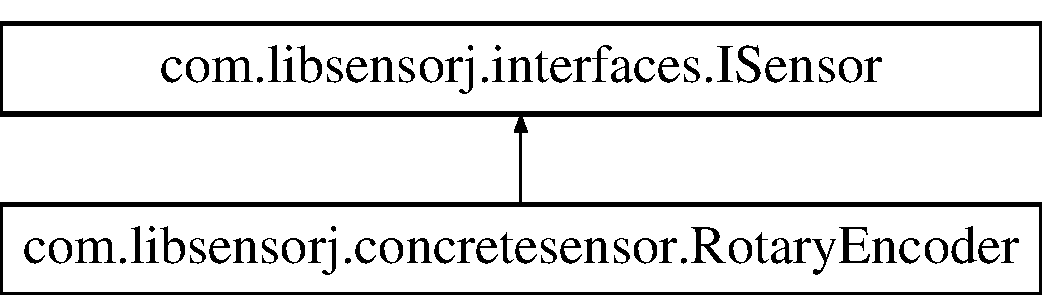
\includegraphics[height=2.000000cm]{classcom_1_1libsensorj_1_1concretesensor_1_1RotaryEncoder}
\end{center}
\end{figure}
\subsection*{Public Member Functions}
\begin{DoxyCompactItemize}
\item 
\hyperlink{classcom_1_1libsensorj_1_1concretesensor_1_1RotaryEncoder_af6db9e02c77d1fe91adbd15162f18c76}{Rotary\+Encoder} ()
\item 
\hyperlink{classcom_1_1libsensorj_1_1concretesensor_1_1RotaryEncoder_a452c852313bec6067e0c564d454e1d2e}{Rotary\+Encoder} (int pin\+A, int pin\+B)
\item 
\hyperlink{classcom_1_1libsensorj_1_1concretesensor_1_1RotaryEncoder_ac3ed9b272a348582d4cb8a25eb49eead}{Rotary\+Encoder} (int pin\+A, int pin\+B, long inital\+Value)
\item 
\hyperlink{classcom_1_1libsensorj_1_1concretesensor_1_1RotaryEncoder_a4590e282d301bc7f6153f47a99ac0a50}{Rotary\+Encoder} (Pin pin\+A, Pin pin\+B, long inital\+Value)
\item 
long \hyperlink{classcom_1_1libsensorj_1_1concretesensor_1_1RotaryEncoder_a8a8c21decdf205abdd445c5f0c8742e4}{get\+Value} ()
\item 
void \hyperlink{classcom_1_1libsensorj_1_1concretesensor_1_1RotaryEncoder_ac8e16c6feadaac8fb338250d86842993}{set\+Listener} (\hyperlink{interfacecom_1_1libsensorj_1_1listeners_1_1RotaryEncoderListener}{Rotary\+Encoder\+Listener} \hyperlink{classcom_1_1libsensorj_1_1concretesensor_1_1RotaryEncoder_ae96674e284081057117e66d9bf2940ea}{listener})
\item 
void \hyperlink{classcom_1_1libsensorj_1_1concretesensor_1_1RotaryEncoder_aa0e07b8e5979b940a4a8bcb96d3af51e}{get\+Instance} ()
\end{DoxyCompactItemize}
\subsection*{Private Member Functions}
\begin{DoxyCompactItemize}
\item 
void \hyperlink{classcom_1_1libsensorj_1_1concretesensor_1_1RotaryEncoder_a86e3fc87eab21e3053cee532b52f7375}{calc\+Encoder\+Value} (int state\+A, int state\+B)
\end{DoxyCompactItemize}
\subsection*{Private Attributes}
\begin{DoxyCompactItemize}
\item 
final Gpio\+Pin\+Digital\+Input \hyperlink{classcom_1_1libsensorj_1_1concretesensor_1_1RotaryEncoder_a8db79599c8930effdf715796115c6739}{input\+A}
\item 
final Gpio\+Pin\+Digital\+Input \hyperlink{classcom_1_1libsensorj_1_1concretesensor_1_1RotaryEncoder_a7245c0e7d71506be358c5d833332630e}{input\+B}
\item 
final Gpio\+Controller \hyperlink{classcom_1_1libsensorj_1_1concretesensor_1_1RotaryEncoder_a689ac7cee2c3bd03c75f50e727943f49}{gpio}
\item 
long \hyperlink{classcom_1_1libsensorj_1_1concretesensor_1_1RotaryEncoder_a4d4be597b70b91b9a24d9f76d6bde510}{encoder\+Value} = 0
\item 
int \hyperlink{classcom_1_1libsensorj_1_1concretesensor_1_1RotaryEncoder_a99d34b4a390d2c2a5eeab7b5fef665ae}{last\+Encoded} = 0
\item 
boolean \hyperlink{classcom_1_1libsensorj_1_1concretesensor_1_1RotaryEncoder_a7b7d95bbeb4dc1a7ad8aeedf550d53f3}{first\+Pass} = true
\item 
\hyperlink{interfacecom_1_1libsensorj_1_1listeners_1_1RotaryEncoderListener}{Rotary\+Encoder\+Listener} \hyperlink{classcom_1_1libsensorj_1_1concretesensor_1_1RotaryEncoder_ae96674e284081057117e66d9bf2940ea}{listener}
\end{DoxyCompactItemize}
\subsection*{Static Private Attributes}
\begin{DoxyCompactItemize}
\item 
static final Pin \hyperlink{classcom_1_1libsensorj_1_1concretesensor_1_1RotaryEncoder_a1b700b49b4e85eb1161d4042f2f57b3d}{D\+E\+F\+A\+U\+L\+T\+\_\+\+P\+I\+N\+\_\+\+A} = Raspi\+Pin.\+G\+P\+I\+O\+\_\+10
\item 
static final Pin \hyperlink{classcom_1_1libsensorj_1_1concretesensor_1_1RotaryEncoder_aaebc5899516aa9385d1ddbb8ed4b12bc}{D\+E\+F\+A\+U\+L\+T\+\_\+\+P\+I\+N\+\_\+\+B} = Raspi\+Pin.\+G\+P\+I\+O\+\_\+08
\item 
static final long \hyperlink{classcom_1_1libsensorj_1_1concretesensor_1_1RotaryEncoder_ad5997b6407cda9bd936b90a82e86458a}{D\+E\+F\+A\+U\+L\+T\+\_\+\+I\+N\+I\+T\+I\+A\+L\+\_\+\+V\+A\+L\+U\+E} = 0
\item 
static final int \hyperlink{classcom_1_1libsensorj_1_1concretesensor_1_1RotaryEncoder_aca1c89ca07e97ca484ae85517660b9f0}{S\+T\+A\+T\+E\+\_\+\+T\+A\+B\+L\+E} \mbox{[}$\,$\mbox{]}\mbox{[}$\,$\mbox{]}
\item 
static final Logger \hyperlink{classcom_1_1libsensorj_1_1concretesensor_1_1RotaryEncoder_a0f4f58edd0f2ed3bf053b3578cfc3a8f}{L\+O\+G\+G\+E\+R} = Log\+Manager.\+get\+Logger(Rotary\+Encoder.\+class.\+get\+Name())
\end{DoxyCompactItemize}


\subsection{Detailed Description}
The Class \hyperlink{classcom_1_1libsensorj_1_1concretesensor_1_1RotaryEncoder}{Rotary\+Encoder}. 

\subsection{Constructor \& Destructor Documentation}
\hypertarget{classcom_1_1libsensorj_1_1concretesensor_1_1RotaryEncoder_af6db9e02c77d1fe91adbd15162f18c76}{}\index{com\+::libsensorj\+::concretesensor\+::\+Rotary\+Encoder@{com\+::libsensorj\+::concretesensor\+::\+Rotary\+Encoder}!Rotary\+Encoder@{Rotary\+Encoder}}
\index{Rotary\+Encoder@{Rotary\+Encoder}!com\+::libsensorj\+::concretesensor\+::\+Rotary\+Encoder@{com\+::libsensorj\+::concretesensor\+::\+Rotary\+Encoder}}
\subsubsection[{Rotary\+Encoder}]{\setlength{\rightskip}{0pt plus 5cm}com.\+libsensorj.\+concretesensor.\+Rotary\+Encoder.\+Rotary\+Encoder (
\begin{DoxyParamCaption}
{}
\end{DoxyParamCaption}
)}\label{classcom_1_1libsensorj_1_1concretesensor_1_1RotaryEncoder_af6db9e02c77d1fe91adbd15162f18c76}
Instantiates a new rotary encoder. \hypertarget{classcom_1_1libsensorj_1_1concretesensor_1_1RotaryEncoder_a452c852313bec6067e0c564d454e1d2e}{}\index{com\+::libsensorj\+::concretesensor\+::\+Rotary\+Encoder@{com\+::libsensorj\+::concretesensor\+::\+Rotary\+Encoder}!Rotary\+Encoder@{Rotary\+Encoder}}
\index{Rotary\+Encoder@{Rotary\+Encoder}!com\+::libsensorj\+::concretesensor\+::\+Rotary\+Encoder@{com\+::libsensorj\+::concretesensor\+::\+Rotary\+Encoder}}
\subsubsection[{Rotary\+Encoder}]{\setlength{\rightskip}{0pt plus 5cm}com.\+libsensorj.\+concretesensor.\+Rotary\+Encoder.\+Rotary\+Encoder (
\begin{DoxyParamCaption}
\item[{int}]{pin\+A, }
\item[{int}]{pin\+B}
\end{DoxyParamCaption}
)}\label{classcom_1_1libsensorj_1_1concretesensor_1_1RotaryEncoder_a452c852313bec6067e0c564d454e1d2e}
Instantiates a new rotary encoder.


\begin{DoxyParams}{Parameters}
{\em pin\+A} & the pin a \\
\hline
{\em pin\+B} & the pin b \\
\hline
\end{DoxyParams}
\hypertarget{classcom_1_1libsensorj_1_1concretesensor_1_1RotaryEncoder_ac3ed9b272a348582d4cb8a25eb49eead}{}\index{com\+::libsensorj\+::concretesensor\+::\+Rotary\+Encoder@{com\+::libsensorj\+::concretesensor\+::\+Rotary\+Encoder}!Rotary\+Encoder@{Rotary\+Encoder}}
\index{Rotary\+Encoder@{Rotary\+Encoder}!com\+::libsensorj\+::concretesensor\+::\+Rotary\+Encoder@{com\+::libsensorj\+::concretesensor\+::\+Rotary\+Encoder}}
\subsubsection[{Rotary\+Encoder}]{\setlength{\rightskip}{0pt plus 5cm}com.\+libsensorj.\+concretesensor.\+Rotary\+Encoder.\+Rotary\+Encoder (
\begin{DoxyParamCaption}
\item[{int}]{pin\+A, }
\item[{int}]{pin\+B, }
\item[{long}]{inital\+Value}
\end{DoxyParamCaption}
)}\label{classcom_1_1libsensorj_1_1concretesensor_1_1RotaryEncoder_ac3ed9b272a348582d4cb8a25eb49eead}
Instantiates a new rotary encoder.


\begin{DoxyParams}{Parameters}
{\em pin\+A} & the pin a \\
\hline
{\em pin\+B} & the pin b \\
\hline
{\em inital\+Value} & the inital value \\
\hline
\end{DoxyParams}
\hypertarget{classcom_1_1libsensorj_1_1concretesensor_1_1RotaryEncoder_a4590e282d301bc7f6153f47a99ac0a50}{}\index{com\+::libsensorj\+::concretesensor\+::\+Rotary\+Encoder@{com\+::libsensorj\+::concretesensor\+::\+Rotary\+Encoder}!Rotary\+Encoder@{Rotary\+Encoder}}
\index{Rotary\+Encoder@{Rotary\+Encoder}!com\+::libsensorj\+::concretesensor\+::\+Rotary\+Encoder@{com\+::libsensorj\+::concretesensor\+::\+Rotary\+Encoder}}
\subsubsection[{Rotary\+Encoder}]{\setlength{\rightskip}{0pt plus 5cm}com.\+libsensorj.\+concretesensor.\+Rotary\+Encoder.\+Rotary\+Encoder (
\begin{DoxyParamCaption}
\item[{Pin}]{pin\+A, }
\item[{Pin}]{pin\+B, }
\item[{long}]{inital\+Value}
\end{DoxyParamCaption}
)}\label{classcom_1_1libsensorj_1_1concretesensor_1_1RotaryEncoder_a4590e282d301bc7f6153f47a99ac0a50}
Instantiates a new rotary encoder.


\begin{DoxyParams}{Parameters}
{\em pin\+A} & the pin a \\
\hline
{\em pin\+B} & the pin b \\
\hline
{\em inital\+Value} & the inital value \\
\hline
\end{DoxyParams}


\subsection{Member Function Documentation}
\hypertarget{classcom_1_1libsensorj_1_1concretesensor_1_1RotaryEncoder_a86e3fc87eab21e3053cee532b52f7375}{}\index{com\+::libsensorj\+::concretesensor\+::\+Rotary\+Encoder@{com\+::libsensorj\+::concretesensor\+::\+Rotary\+Encoder}!calc\+Encoder\+Value@{calc\+Encoder\+Value}}
\index{calc\+Encoder\+Value@{calc\+Encoder\+Value}!com\+::libsensorj\+::concretesensor\+::\+Rotary\+Encoder@{com\+::libsensorj\+::concretesensor\+::\+Rotary\+Encoder}}
\subsubsection[{calc\+Encoder\+Value}]{\setlength{\rightskip}{0pt plus 5cm}void com.\+libsensorj.\+concretesensor.\+Rotary\+Encoder.\+calc\+Encoder\+Value (
\begin{DoxyParamCaption}
\item[{int}]{state\+A, }
\item[{int}]{state\+B}
\end{DoxyParamCaption}
)\hspace{0.3cm}{\ttfamily [private]}}\label{classcom_1_1libsensorj_1_1concretesensor_1_1RotaryEncoder_a86e3fc87eab21e3053cee532b52f7375}
Calc encoder value.


\begin{DoxyParams}{Parameters}
{\em state\+A} & the state a \\
\hline
{\em state\+B} & the state b \\
\hline
\end{DoxyParams}
\hypertarget{classcom_1_1libsensorj_1_1concretesensor_1_1RotaryEncoder_aa0e07b8e5979b940a4a8bcb96d3af51e}{}\index{com\+::libsensorj\+::concretesensor\+::\+Rotary\+Encoder@{com\+::libsensorj\+::concretesensor\+::\+Rotary\+Encoder}!get\+Instance@{get\+Instance}}
\index{get\+Instance@{get\+Instance}!com\+::libsensorj\+::concretesensor\+::\+Rotary\+Encoder@{com\+::libsensorj\+::concretesensor\+::\+Rotary\+Encoder}}
\subsubsection[{get\+Instance}]{\setlength{\rightskip}{0pt plus 5cm}void com.\+libsensorj.\+concretesensor.\+Rotary\+Encoder.\+get\+Instance (
\begin{DoxyParamCaption}
{}
\end{DoxyParamCaption}
)}\label{classcom_1_1libsensorj_1_1concretesensor_1_1RotaryEncoder_aa0e07b8e5979b940a4a8bcb96d3af51e}
Gets the single instance of I\+Sensor.

\begin{DoxyReturn}{Returns}
single instance of I\+Sensor 
\end{DoxyReturn}


Implements \hyperlink{interfacecom_1_1libsensorj_1_1interfaces_1_1ISensor_a3c3db93a33adecde81a528651790f75e}{com.\+libsensorj.\+interfaces.\+I\+Sensor}.

\hypertarget{classcom_1_1libsensorj_1_1concretesensor_1_1RotaryEncoder_a8a8c21decdf205abdd445c5f0c8742e4}{}\index{com\+::libsensorj\+::concretesensor\+::\+Rotary\+Encoder@{com\+::libsensorj\+::concretesensor\+::\+Rotary\+Encoder}!get\+Value@{get\+Value}}
\index{get\+Value@{get\+Value}!com\+::libsensorj\+::concretesensor\+::\+Rotary\+Encoder@{com\+::libsensorj\+::concretesensor\+::\+Rotary\+Encoder}}
\subsubsection[{get\+Value}]{\setlength{\rightskip}{0pt plus 5cm}long com.\+libsensorj.\+concretesensor.\+Rotary\+Encoder.\+get\+Value (
\begin{DoxyParamCaption}
{}
\end{DoxyParamCaption}
)}\label{classcom_1_1libsensorj_1_1concretesensor_1_1RotaryEncoder_a8a8c21decdf205abdd445c5f0c8742e4}
Gets the value.

\begin{DoxyReturn}{Returns}
the value 
\end{DoxyReturn}
\hypertarget{classcom_1_1libsensorj_1_1concretesensor_1_1RotaryEncoder_ac8e16c6feadaac8fb338250d86842993}{}\index{com\+::libsensorj\+::concretesensor\+::\+Rotary\+Encoder@{com\+::libsensorj\+::concretesensor\+::\+Rotary\+Encoder}!set\+Listener@{set\+Listener}}
\index{set\+Listener@{set\+Listener}!com\+::libsensorj\+::concretesensor\+::\+Rotary\+Encoder@{com\+::libsensorj\+::concretesensor\+::\+Rotary\+Encoder}}
\subsubsection[{set\+Listener}]{\setlength{\rightskip}{0pt plus 5cm}void com.\+libsensorj.\+concretesensor.\+Rotary\+Encoder.\+set\+Listener (
\begin{DoxyParamCaption}
\item[{{\bf Rotary\+Encoder\+Listener}}]{listener}
\end{DoxyParamCaption}
)}\label{classcom_1_1libsensorj_1_1concretesensor_1_1RotaryEncoder_ac8e16c6feadaac8fb338250d86842993}
Sets the listener.


\begin{DoxyParams}{Parameters}
{\em listener} & the new listener \\
\hline
\end{DoxyParams}


\subsection{Member Data Documentation}
\hypertarget{classcom_1_1libsensorj_1_1concretesensor_1_1RotaryEncoder_ad5997b6407cda9bd936b90a82e86458a}{}\index{com\+::libsensorj\+::concretesensor\+::\+Rotary\+Encoder@{com\+::libsensorj\+::concretesensor\+::\+Rotary\+Encoder}!D\+E\+F\+A\+U\+L\+T\+\_\+\+I\+N\+I\+T\+I\+A\+L\+\_\+\+V\+A\+L\+U\+E@{D\+E\+F\+A\+U\+L\+T\+\_\+\+I\+N\+I\+T\+I\+A\+L\+\_\+\+V\+A\+L\+U\+E}}
\index{D\+E\+F\+A\+U\+L\+T\+\_\+\+I\+N\+I\+T\+I\+A\+L\+\_\+\+V\+A\+L\+U\+E@{D\+E\+F\+A\+U\+L\+T\+\_\+\+I\+N\+I\+T\+I\+A\+L\+\_\+\+V\+A\+L\+U\+E}!com\+::libsensorj\+::concretesensor\+::\+Rotary\+Encoder@{com\+::libsensorj\+::concretesensor\+::\+Rotary\+Encoder}}
\subsubsection[{D\+E\+F\+A\+U\+L\+T\+\_\+\+I\+N\+I\+T\+I\+A\+L\+\_\+\+V\+A\+L\+U\+E}]{\setlength{\rightskip}{0pt plus 5cm}final long com.\+libsensorj.\+concretesensor.\+Rotary\+Encoder.\+D\+E\+F\+A\+U\+L\+T\+\_\+\+I\+N\+I\+T\+I\+A\+L\+\_\+\+V\+A\+L\+U\+E = 0\hspace{0.3cm}{\ttfamily [static]}, {\ttfamily [private]}}\label{classcom_1_1libsensorj_1_1concretesensor_1_1RotaryEncoder_ad5997b6407cda9bd936b90a82e86458a}
The Constant D\+E\+F\+A\+U\+L\+T\+\_\+\+I\+N\+I\+T\+I\+A\+L\+\_\+\+V\+A\+L\+U\+E. \hypertarget{classcom_1_1libsensorj_1_1concretesensor_1_1RotaryEncoder_a1b700b49b4e85eb1161d4042f2f57b3d}{}\index{com\+::libsensorj\+::concretesensor\+::\+Rotary\+Encoder@{com\+::libsensorj\+::concretesensor\+::\+Rotary\+Encoder}!D\+E\+F\+A\+U\+L\+T\+\_\+\+P\+I\+N\+\_\+\+A@{D\+E\+F\+A\+U\+L\+T\+\_\+\+P\+I\+N\+\_\+\+A}}
\index{D\+E\+F\+A\+U\+L\+T\+\_\+\+P\+I\+N\+\_\+\+A@{D\+E\+F\+A\+U\+L\+T\+\_\+\+P\+I\+N\+\_\+\+A}!com\+::libsensorj\+::concretesensor\+::\+Rotary\+Encoder@{com\+::libsensorj\+::concretesensor\+::\+Rotary\+Encoder}}
\subsubsection[{D\+E\+F\+A\+U\+L\+T\+\_\+\+P\+I\+N\+\_\+\+A}]{\setlength{\rightskip}{0pt plus 5cm}final Pin com.\+libsensorj.\+concretesensor.\+Rotary\+Encoder.\+D\+E\+F\+A\+U\+L\+T\+\_\+\+P\+I\+N\+\_\+\+A = Raspi\+Pin.\+G\+P\+I\+O\+\_\+10\hspace{0.3cm}{\ttfamily [static]}, {\ttfamily [private]}}\label{classcom_1_1libsensorj_1_1concretesensor_1_1RotaryEncoder_a1b700b49b4e85eb1161d4042f2f57b3d}
The Constant D\+E\+F\+A\+U\+L\+T\+\_\+\+P\+I\+N\+\_\+\+A. \hypertarget{classcom_1_1libsensorj_1_1concretesensor_1_1RotaryEncoder_aaebc5899516aa9385d1ddbb8ed4b12bc}{}\index{com\+::libsensorj\+::concretesensor\+::\+Rotary\+Encoder@{com\+::libsensorj\+::concretesensor\+::\+Rotary\+Encoder}!D\+E\+F\+A\+U\+L\+T\+\_\+\+P\+I\+N\+\_\+\+B@{D\+E\+F\+A\+U\+L\+T\+\_\+\+P\+I\+N\+\_\+\+B}}
\index{D\+E\+F\+A\+U\+L\+T\+\_\+\+P\+I\+N\+\_\+\+B@{D\+E\+F\+A\+U\+L\+T\+\_\+\+P\+I\+N\+\_\+\+B}!com\+::libsensorj\+::concretesensor\+::\+Rotary\+Encoder@{com\+::libsensorj\+::concretesensor\+::\+Rotary\+Encoder}}
\subsubsection[{D\+E\+F\+A\+U\+L\+T\+\_\+\+P\+I\+N\+\_\+\+B}]{\setlength{\rightskip}{0pt plus 5cm}final Pin com.\+libsensorj.\+concretesensor.\+Rotary\+Encoder.\+D\+E\+F\+A\+U\+L\+T\+\_\+\+P\+I\+N\+\_\+\+B = Raspi\+Pin.\+G\+P\+I\+O\+\_\+08\hspace{0.3cm}{\ttfamily [static]}, {\ttfamily [private]}}\label{classcom_1_1libsensorj_1_1concretesensor_1_1RotaryEncoder_aaebc5899516aa9385d1ddbb8ed4b12bc}
The Constant D\+E\+F\+A\+U\+L\+T\+\_\+\+P\+I\+N\+\_\+\+B. \hypertarget{classcom_1_1libsensorj_1_1concretesensor_1_1RotaryEncoder_a4d4be597b70b91b9a24d9f76d6bde510}{}\index{com\+::libsensorj\+::concretesensor\+::\+Rotary\+Encoder@{com\+::libsensorj\+::concretesensor\+::\+Rotary\+Encoder}!encoder\+Value@{encoder\+Value}}
\index{encoder\+Value@{encoder\+Value}!com\+::libsensorj\+::concretesensor\+::\+Rotary\+Encoder@{com\+::libsensorj\+::concretesensor\+::\+Rotary\+Encoder}}
\subsubsection[{encoder\+Value}]{\setlength{\rightskip}{0pt plus 5cm}long com.\+libsensorj.\+concretesensor.\+Rotary\+Encoder.\+encoder\+Value = 0\hspace{0.3cm}{\ttfamily [private]}}\label{classcom_1_1libsensorj_1_1concretesensor_1_1RotaryEncoder_a4d4be597b70b91b9a24d9f76d6bde510}
The encoder value. \hypertarget{classcom_1_1libsensorj_1_1concretesensor_1_1RotaryEncoder_a7b7d95bbeb4dc1a7ad8aeedf550d53f3}{}\index{com\+::libsensorj\+::concretesensor\+::\+Rotary\+Encoder@{com\+::libsensorj\+::concretesensor\+::\+Rotary\+Encoder}!first\+Pass@{first\+Pass}}
\index{first\+Pass@{first\+Pass}!com\+::libsensorj\+::concretesensor\+::\+Rotary\+Encoder@{com\+::libsensorj\+::concretesensor\+::\+Rotary\+Encoder}}
\subsubsection[{first\+Pass}]{\setlength{\rightskip}{0pt plus 5cm}boolean com.\+libsensorj.\+concretesensor.\+Rotary\+Encoder.\+first\+Pass = true\hspace{0.3cm}{\ttfamily [private]}}\label{classcom_1_1libsensorj_1_1concretesensor_1_1RotaryEncoder_a7b7d95bbeb4dc1a7ad8aeedf550d53f3}
The first pass. \hypertarget{classcom_1_1libsensorj_1_1concretesensor_1_1RotaryEncoder_a689ac7cee2c3bd03c75f50e727943f49}{}\index{com\+::libsensorj\+::concretesensor\+::\+Rotary\+Encoder@{com\+::libsensorj\+::concretesensor\+::\+Rotary\+Encoder}!gpio@{gpio}}
\index{gpio@{gpio}!com\+::libsensorj\+::concretesensor\+::\+Rotary\+Encoder@{com\+::libsensorj\+::concretesensor\+::\+Rotary\+Encoder}}
\subsubsection[{gpio}]{\setlength{\rightskip}{0pt plus 5cm}final Gpio\+Controller com.\+libsensorj.\+concretesensor.\+Rotary\+Encoder.\+gpio\hspace{0.3cm}{\ttfamily [private]}}\label{classcom_1_1libsensorj_1_1concretesensor_1_1RotaryEncoder_a689ac7cee2c3bd03c75f50e727943f49}
The gpio. \hypertarget{classcom_1_1libsensorj_1_1concretesensor_1_1RotaryEncoder_a8db79599c8930effdf715796115c6739}{}\index{com\+::libsensorj\+::concretesensor\+::\+Rotary\+Encoder@{com\+::libsensorj\+::concretesensor\+::\+Rotary\+Encoder}!input\+A@{input\+A}}
\index{input\+A@{input\+A}!com\+::libsensorj\+::concretesensor\+::\+Rotary\+Encoder@{com\+::libsensorj\+::concretesensor\+::\+Rotary\+Encoder}}
\subsubsection[{input\+A}]{\setlength{\rightskip}{0pt plus 5cm}final Gpio\+Pin\+Digital\+Input com.\+libsensorj.\+concretesensor.\+Rotary\+Encoder.\+input\+A\hspace{0.3cm}{\ttfamily [private]}}\label{classcom_1_1libsensorj_1_1concretesensor_1_1RotaryEncoder_a8db79599c8930effdf715796115c6739}
The input a. \hypertarget{classcom_1_1libsensorj_1_1concretesensor_1_1RotaryEncoder_a7245c0e7d71506be358c5d833332630e}{}\index{com\+::libsensorj\+::concretesensor\+::\+Rotary\+Encoder@{com\+::libsensorj\+::concretesensor\+::\+Rotary\+Encoder}!input\+B@{input\+B}}
\index{input\+B@{input\+B}!com\+::libsensorj\+::concretesensor\+::\+Rotary\+Encoder@{com\+::libsensorj\+::concretesensor\+::\+Rotary\+Encoder}}
\subsubsection[{input\+B}]{\setlength{\rightskip}{0pt plus 5cm}final Gpio\+Pin\+Digital\+Input com.\+libsensorj.\+concretesensor.\+Rotary\+Encoder.\+input\+B\hspace{0.3cm}{\ttfamily [private]}}\label{classcom_1_1libsensorj_1_1concretesensor_1_1RotaryEncoder_a7245c0e7d71506be358c5d833332630e}
The input b. \hypertarget{classcom_1_1libsensorj_1_1concretesensor_1_1RotaryEncoder_a99d34b4a390d2c2a5eeab7b5fef665ae}{}\index{com\+::libsensorj\+::concretesensor\+::\+Rotary\+Encoder@{com\+::libsensorj\+::concretesensor\+::\+Rotary\+Encoder}!last\+Encoded@{last\+Encoded}}
\index{last\+Encoded@{last\+Encoded}!com\+::libsensorj\+::concretesensor\+::\+Rotary\+Encoder@{com\+::libsensorj\+::concretesensor\+::\+Rotary\+Encoder}}
\subsubsection[{last\+Encoded}]{\setlength{\rightskip}{0pt plus 5cm}int com.\+libsensorj.\+concretesensor.\+Rotary\+Encoder.\+last\+Encoded = 0\hspace{0.3cm}{\ttfamily [private]}}\label{classcom_1_1libsensorj_1_1concretesensor_1_1RotaryEncoder_a99d34b4a390d2c2a5eeab7b5fef665ae}
The last encoded. \hypertarget{classcom_1_1libsensorj_1_1concretesensor_1_1RotaryEncoder_ae96674e284081057117e66d9bf2940ea}{}\index{com\+::libsensorj\+::concretesensor\+::\+Rotary\+Encoder@{com\+::libsensorj\+::concretesensor\+::\+Rotary\+Encoder}!listener@{listener}}
\index{listener@{listener}!com\+::libsensorj\+::concretesensor\+::\+Rotary\+Encoder@{com\+::libsensorj\+::concretesensor\+::\+Rotary\+Encoder}}
\subsubsection[{listener}]{\setlength{\rightskip}{0pt plus 5cm}{\bf Rotary\+Encoder\+Listener} com.\+libsensorj.\+concretesensor.\+Rotary\+Encoder.\+listener\hspace{0.3cm}{\ttfamily [private]}}\label{classcom_1_1libsensorj_1_1concretesensor_1_1RotaryEncoder_ae96674e284081057117e66d9bf2940ea}
The listener. \hypertarget{classcom_1_1libsensorj_1_1concretesensor_1_1RotaryEncoder_a0f4f58edd0f2ed3bf053b3578cfc3a8f}{}\index{com\+::libsensorj\+::concretesensor\+::\+Rotary\+Encoder@{com\+::libsensorj\+::concretesensor\+::\+Rotary\+Encoder}!L\+O\+G\+G\+E\+R@{L\+O\+G\+G\+E\+R}}
\index{L\+O\+G\+G\+E\+R@{L\+O\+G\+G\+E\+R}!com\+::libsensorj\+::concretesensor\+::\+Rotary\+Encoder@{com\+::libsensorj\+::concretesensor\+::\+Rotary\+Encoder}}
\subsubsection[{L\+O\+G\+G\+E\+R}]{\setlength{\rightskip}{0pt plus 5cm}final Logger com.\+libsensorj.\+concretesensor.\+Rotary\+Encoder.\+L\+O\+G\+G\+E\+R = Log\+Manager.\+get\+Logger(Rotary\+Encoder.\+class.\+get\+Name())\hspace{0.3cm}{\ttfamily [static]}, {\ttfamily [private]}}\label{classcom_1_1libsensorj_1_1concretesensor_1_1RotaryEncoder_a0f4f58edd0f2ed3bf053b3578cfc3a8f}
The Constant L\+O\+G\+G\+E\+R. \hypertarget{classcom_1_1libsensorj_1_1concretesensor_1_1RotaryEncoder_aca1c89ca07e97ca484ae85517660b9f0}{}\index{com\+::libsensorj\+::concretesensor\+::\+Rotary\+Encoder@{com\+::libsensorj\+::concretesensor\+::\+Rotary\+Encoder}!S\+T\+A\+T\+E\+\_\+\+T\+A\+B\+L\+E@{S\+T\+A\+T\+E\+\_\+\+T\+A\+B\+L\+E}}
\index{S\+T\+A\+T\+E\+\_\+\+T\+A\+B\+L\+E@{S\+T\+A\+T\+E\+\_\+\+T\+A\+B\+L\+E}!com\+::libsensorj\+::concretesensor\+::\+Rotary\+Encoder@{com\+::libsensorj\+::concretesensor\+::\+Rotary\+Encoder}}
\subsubsection[{S\+T\+A\+T\+E\+\_\+\+T\+A\+B\+L\+E}]{\setlength{\rightskip}{0pt plus 5cm}final int com.\+libsensorj.\+concretesensor.\+Rotary\+Encoder.\+S\+T\+A\+T\+E\+\_\+\+T\+A\+B\+L\+E\mbox{[}$\,$\mbox{]}\mbox{[}$\,$\mbox{]}\hspace{0.3cm}{\ttfamily [static]}, {\ttfamily [private]}}\label{classcom_1_1libsensorj_1_1concretesensor_1_1RotaryEncoder_aca1c89ca07e97ca484ae85517660b9f0}
{\bfseries Initial value\+:}
\begin{DoxyCode}
= \{
        \{0, 1, 1, -1\},
        \{-1, 0, 1, -1\},
        \{-1, 1, 0, -1\},
        \{-1, 1, 1, 0\}
    \}
\end{DoxyCode}
The Constant S\+T\+A\+T\+E\+\_\+\+T\+A\+B\+L\+E. 

The documentation for this class was generated from the following file\+:\begin{DoxyCompactItemize}
\item 
main/java/com/libsensorj/concretesensor/\hyperlink{RotaryEncoder_8java}{Rotary\+Encoder.\+java}\end{DoxyCompactItemize}

\hypertarget{classcom_1_1libsensorj_1_1concretefactory_1_1RotaryEncoderFactory}{}\section{com.\+libsensorj.\+concretefactory.\+Rotary\+Encoder\+Factory Class Reference}
\label{classcom_1_1libsensorj_1_1concretefactory_1_1RotaryEncoderFactory}\index{com.\+libsensorj.\+concretefactory.\+Rotary\+Encoder\+Factory@{com.\+libsensorj.\+concretefactory.\+Rotary\+Encoder\+Factory}}
Inheritance diagram for com.\+libsensorj.\+concretefactory.\+Rotary\+Encoder\+Factory\+:\begin{figure}[H]
\begin{center}
\leavevmode
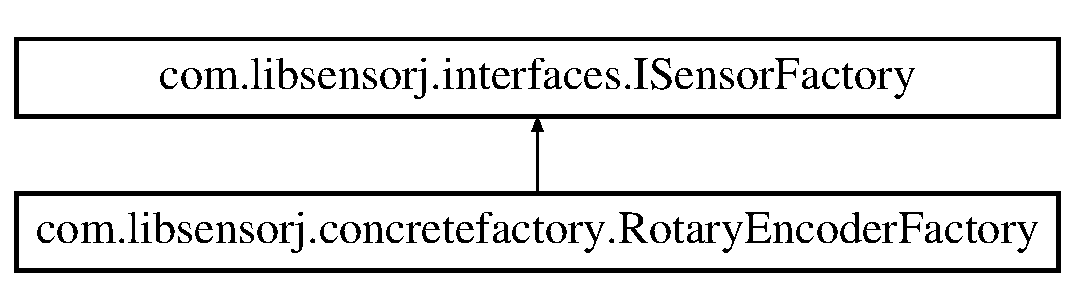
\includegraphics[height=2.000000cm]{classcom_1_1libsensorj_1_1concretefactory_1_1RotaryEncoderFactory}
\end{center}
\end{figure}
\subsection*{Public Member Functions}
\begin{DoxyCompactItemize}
\item 
\hyperlink{interfacecom_1_1libsensorj_1_1interfaces_1_1ISensor}{I\+Sensor} \hyperlink{classcom_1_1libsensorj_1_1concretefactory_1_1RotaryEncoderFactory_a5f9c404d9b61d8aaf63cad82b87becd7}{create\+Sensor} ()
\item 
\hyperlink{classcom_1_1libsensorj_1_1interfaces_1_1IEvent}{I\+Event} \hyperlink{classcom_1_1libsensorj_1_1concretefactory_1_1RotaryEncoderFactory_a8f36c2cbdddcd1c71d438efafc73ffc2}{create\+Event} ()
\end{DoxyCompactItemize}


\subsection{Detailed Description}
A factory for creating Rotary\+Encoder objects. 

\subsection{Member Function Documentation}
\hypertarget{classcom_1_1libsensorj_1_1concretefactory_1_1RotaryEncoderFactory_a8f36c2cbdddcd1c71d438efafc73ffc2}{}\index{com\+::libsensorj\+::concretefactory\+::\+Rotary\+Encoder\+Factory@{com\+::libsensorj\+::concretefactory\+::\+Rotary\+Encoder\+Factory}!create\+Event@{create\+Event}}
\index{create\+Event@{create\+Event}!com\+::libsensorj\+::concretefactory\+::\+Rotary\+Encoder\+Factory@{com\+::libsensorj\+::concretefactory\+::\+Rotary\+Encoder\+Factory}}
\subsubsection[{create\+Event}]{\setlength{\rightskip}{0pt plus 5cm}{\bf I\+Event} com.\+libsensorj.\+concretefactory.\+Rotary\+Encoder\+Factory.\+create\+Event (
\begin{DoxyParamCaption}
{}
\end{DoxyParamCaption}
)}\label{classcom_1_1libsensorj_1_1concretefactory_1_1RotaryEncoderFactory_a8f36c2cbdddcd1c71d438efafc73ffc2}
Creates a new I\+Event object.

\begin{DoxyReturn}{Returns}
the I\+Event 
\end{DoxyReturn}


Implements \hyperlink{interfacecom_1_1libsensorj_1_1interfaces_1_1ISensorFactory_a2b074d01287a4e64677097255ba9e768}{com.\+libsensorj.\+interfaces.\+I\+Sensor\+Factory}.

\hypertarget{classcom_1_1libsensorj_1_1concretefactory_1_1RotaryEncoderFactory_a5f9c404d9b61d8aaf63cad82b87becd7}{}\index{com\+::libsensorj\+::concretefactory\+::\+Rotary\+Encoder\+Factory@{com\+::libsensorj\+::concretefactory\+::\+Rotary\+Encoder\+Factory}!create\+Sensor@{create\+Sensor}}
\index{create\+Sensor@{create\+Sensor}!com\+::libsensorj\+::concretefactory\+::\+Rotary\+Encoder\+Factory@{com\+::libsensorj\+::concretefactory\+::\+Rotary\+Encoder\+Factory}}
\subsubsection[{create\+Sensor}]{\setlength{\rightskip}{0pt plus 5cm}{\bf I\+Sensor} com.\+libsensorj.\+concretefactory.\+Rotary\+Encoder\+Factory.\+create\+Sensor (
\begin{DoxyParamCaption}
{}
\end{DoxyParamCaption}
)}\label{classcom_1_1libsensorj_1_1concretefactory_1_1RotaryEncoderFactory_a5f9c404d9b61d8aaf63cad82b87becd7}
Creates a new I\+Sensor object.

\begin{DoxyReturn}{Returns}
the I\+Sensor 
\end{DoxyReturn}


Implements \hyperlink{interfacecom_1_1libsensorj_1_1interfaces_1_1ISensorFactory_ac14c6d566c37c6a79c6db1e85634f25d}{com.\+libsensorj.\+interfaces.\+I\+Sensor\+Factory}.



The documentation for this class was generated from the following file\+:\begin{DoxyCompactItemize}
\item 
main/java/com/libsensorj/concretefactory/\hyperlink{RotaryEncoderFactory_8java}{Rotary\+Encoder\+Factory.\+java}\end{DoxyCompactItemize}

\hypertarget{interfacecom_1_1libsensorj_1_1listeners_1_1RotaryEncoderListener}{}\section{com.\+libsensorj.\+listeners.\+Rotary\+Encoder\+Listener Interface Reference}
\label{interfacecom_1_1libsensorj_1_1listeners_1_1RotaryEncoderListener}\index{com.\+libsensorj.\+listeners.\+Rotary\+Encoder\+Listener@{com.\+libsensorj.\+listeners.\+Rotary\+Encoder\+Listener}}
Inheritance diagram for com.\+libsensorj.\+listeners.\+Rotary\+Encoder\+Listener\+:\begin{figure}[H]
\begin{center}
\leavevmode
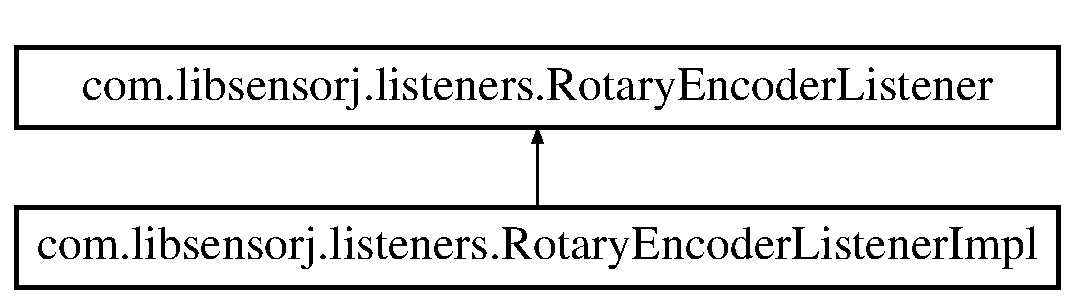
\includegraphics[height=2.000000cm]{interfacecom_1_1libsensorj_1_1listeners_1_1RotaryEncoderListener}
\end{center}
\end{figure}
\subsection*{Public Member Functions}
\begin{DoxyCompactItemize}
\item 
void \hyperlink{interfacecom_1_1libsensorj_1_1listeners_1_1RotaryEncoderListener_a0b7b75d6b0a30c31bd69e1674b1c98ec}{turned\+Clockwise} (long encoder\+Value)
\item 
void \hyperlink{interfacecom_1_1libsensorj_1_1listeners_1_1RotaryEncoderListener_aa04a814b5886e2fd2c095a8c2827b6a8}{turned\+Counterclockwise} (long encoder\+Value)
\end{DoxyCompactItemize}


\subsection{Detailed Description}
The listener interface for receiving rotary\+Encoder events. The class that is interested in processing a rotary\+Encoder event implements this interface, and the object created with that class is registered with a component using the component's {\ttfamily add\+Rotary\+Encoder\+Listener{\ttfamily  method. When the rotary\+Encoder event occurs, that object's appropriate method is invoked.}}

{\ttfamily {\ttfamily \begin{DoxySeeAlso}{See also}
Rotary\+Encoder\+Event 
\end{DoxySeeAlso}
}}

\subsection{Member Function Documentation}
\hypertarget{interfacecom_1_1libsensorj_1_1listeners_1_1RotaryEncoderListener_a0b7b75d6b0a30c31bd69e1674b1c98ec}{}\index{com\+::libsensorj\+::listeners\+::\+Rotary\+Encoder\+Listener@{com\+::libsensorj\+::listeners\+::\+Rotary\+Encoder\+Listener}!turned\+Clockwise@{turned\+Clockwise}}
\index{turned\+Clockwise@{turned\+Clockwise}!com\+::libsensorj\+::listeners\+::\+Rotary\+Encoder\+Listener@{com\+::libsensorj\+::listeners\+::\+Rotary\+Encoder\+Listener}}
\subsubsection[{turned\+Clockwise}]{\setlength{\rightskip}{0pt plus 5cm}void com.\+libsensorj.\+listeners.\+Rotary\+Encoder\+Listener.\+turned\+Clockwise (
\begin{DoxyParamCaption}
\item[{long}]{encoder\+Value}
\end{DoxyParamCaption}
)}\label{interfacecom_1_1libsensorj_1_1listeners_1_1RotaryEncoderListener_a0b7b75d6b0a30c31bd69e1674b1c98ec}
Turned clockwise.


\begin{DoxyParams}{Parameters}
{\em encoder\+Value} & the encoder value \\
\hline
\end{DoxyParams}


Implemented in \hyperlink{classcom_1_1libsensorj_1_1listeners_1_1RotaryEncoderListenerImpl_a3dbffe8a20820933fc5910d0aecf5212}{com.\+libsensorj.\+listeners.\+Rotary\+Encoder\+Listener\+Impl}.

\hypertarget{interfacecom_1_1libsensorj_1_1listeners_1_1RotaryEncoderListener_aa04a814b5886e2fd2c095a8c2827b6a8}{}\index{com\+::libsensorj\+::listeners\+::\+Rotary\+Encoder\+Listener@{com\+::libsensorj\+::listeners\+::\+Rotary\+Encoder\+Listener}!turned\+Counterclockwise@{turned\+Counterclockwise}}
\index{turned\+Counterclockwise@{turned\+Counterclockwise}!com\+::libsensorj\+::listeners\+::\+Rotary\+Encoder\+Listener@{com\+::libsensorj\+::listeners\+::\+Rotary\+Encoder\+Listener}}
\subsubsection[{turned\+Counterclockwise}]{\setlength{\rightskip}{0pt plus 5cm}void com.\+libsensorj.\+listeners.\+Rotary\+Encoder\+Listener.\+turned\+Counterclockwise (
\begin{DoxyParamCaption}
\item[{long}]{encoder\+Value}
\end{DoxyParamCaption}
)}\label{interfacecom_1_1libsensorj_1_1listeners_1_1RotaryEncoderListener_aa04a814b5886e2fd2c095a8c2827b6a8}
Turned counterclockwise.


\begin{DoxyParams}{Parameters}
{\em encoder\+Value} & the encoder value \\
\hline
\end{DoxyParams}


Implemented in \hyperlink{classcom_1_1libsensorj_1_1listeners_1_1RotaryEncoderListenerImpl_a7c07901b6fbfe89c7406afa8fcf4d482}{com.\+libsensorj.\+listeners.\+Rotary\+Encoder\+Listener\+Impl}.



The documentation for this interface was generated from the following file\+:\begin{DoxyCompactItemize}
\item 
main/java/com/libsensorj/listeners/\hyperlink{RotaryEncoderListener_8java}{Rotary\+Encoder\+Listener.\+java}\end{DoxyCompactItemize}

\hypertarget{classcom_1_1libsensorj_1_1listeners_1_1RotaryEncoderListenerImpl}{}\section{com.\+libsensorj.\+listeners.\+Rotary\+Encoder\+Listener\+Impl Class Reference}
\label{classcom_1_1libsensorj_1_1listeners_1_1RotaryEncoderListenerImpl}\index{com.\+libsensorj.\+listeners.\+Rotary\+Encoder\+Listener\+Impl@{com.\+libsensorj.\+listeners.\+Rotary\+Encoder\+Listener\+Impl}}
Inheritance diagram for com.\+libsensorj.\+listeners.\+Rotary\+Encoder\+Listener\+Impl\+:\begin{figure}[H]
\begin{center}
\leavevmode
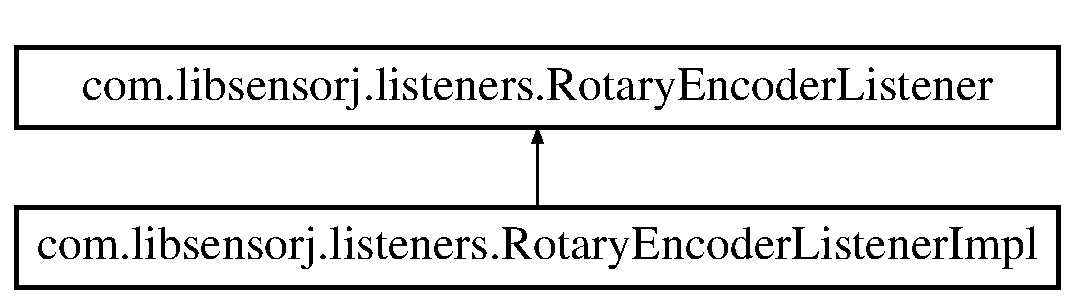
\includegraphics[height=2.000000cm]{classcom_1_1libsensorj_1_1listeners_1_1RotaryEncoderListenerImpl}
\end{center}
\end{figure}
\subsection*{Public Member Functions}
\begin{DoxyCompactItemize}
\item 
void \hyperlink{classcom_1_1libsensorj_1_1listeners_1_1RotaryEncoderListenerImpl_a3dbffe8a20820933fc5910d0aecf5212}{turned\+Clockwise} (long encoder\+Value)
\item 
void \hyperlink{classcom_1_1libsensorj_1_1listeners_1_1RotaryEncoderListenerImpl_a7c07901b6fbfe89c7406afa8fcf4d482}{turned\+Counterclockwise} (long encoder\+Value)
\end{DoxyCompactItemize}
\subsection*{Static Private Attributes}
\begin{DoxyCompactItemize}
\item 
static final Logger \hyperlink{classcom_1_1libsensorj_1_1listeners_1_1RotaryEncoderListenerImpl_af88de2de8fdc7d0d31d454648560aa41}{L\+O\+G\+G\+E\+R}
\end{DoxyCompactItemize}


\subsection{Detailed Description}
The Class \hyperlink{classcom_1_1libsensorj_1_1listeners_1_1RotaryEncoderListenerImpl}{Rotary\+Encoder\+Listener\+Impl}. 

\subsection{Member Function Documentation}
\hypertarget{classcom_1_1libsensorj_1_1listeners_1_1RotaryEncoderListenerImpl_a3dbffe8a20820933fc5910d0aecf5212}{}\index{com\+::libsensorj\+::listeners\+::\+Rotary\+Encoder\+Listener\+Impl@{com\+::libsensorj\+::listeners\+::\+Rotary\+Encoder\+Listener\+Impl}!turned\+Clockwise@{turned\+Clockwise}}
\index{turned\+Clockwise@{turned\+Clockwise}!com\+::libsensorj\+::listeners\+::\+Rotary\+Encoder\+Listener\+Impl@{com\+::libsensorj\+::listeners\+::\+Rotary\+Encoder\+Listener\+Impl}}
\subsubsection[{turned\+Clockwise}]{\setlength{\rightskip}{0pt plus 5cm}void com.\+libsensorj.\+listeners.\+Rotary\+Encoder\+Listener\+Impl.\+turned\+Clockwise (
\begin{DoxyParamCaption}
\item[{long}]{encoder\+Value}
\end{DoxyParamCaption}
)}\label{classcom_1_1libsensorj_1_1listeners_1_1RotaryEncoderListenerImpl_a3dbffe8a20820933fc5910d0aecf5212}
Turned clockwise.


\begin{DoxyParams}{Parameters}
{\em encoder\+Value} & the encoder value \\
\hline
\end{DoxyParams}


Implements \hyperlink{interfacecom_1_1libsensorj_1_1listeners_1_1RotaryEncoderListener_a0b7b75d6b0a30c31bd69e1674b1c98ec}{com.\+libsensorj.\+listeners.\+Rotary\+Encoder\+Listener}.

\hypertarget{classcom_1_1libsensorj_1_1listeners_1_1RotaryEncoderListenerImpl_a7c07901b6fbfe89c7406afa8fcf4d482}{}\index{com\+::libsensorj\+::listeners\+::\+Rotary\+Encoder\+Listener\+Impl@{com\+::libsensorj\+::listeners\+::\+Rotary\+Encoder\+Listener\+Impl}!turned\+Counterclockwise@{turned\+Counterclockwise}}
\index{turned\+Counterclockwise@{turned\+Counterclockwise}!com\+::libsensorj\+::listeners\+::\+Rotary\+Encoder\+Listener\+Impl@{com\+::libsensorj\+::listeners\+::\+Rotary\+Encoder\+Listener\+Impl}}
\subsubsection[{turned\+Counterclockwise}]{\setlength{\rightskip}{0pt plus 5cm}void com.\+libsensorj.\+listeners.\+Rotary\+Encoder\+Listener\+Impl.\+turned\+Counterclockwise (
\begin{DoxyParamCaption}
\item[{long}]{encoder\+Value}
\end{DoxyParamCaption}
)}\label{classcom_1_1libsensorj_1_1listeners_1_1RotaryEncoderListenerImpl_a7c07901b6fbfe89c7406afa8fcf4d482}
Turned counterclockwise.


\begin{DoxyParams}{Parameters}
{\em encoder\+Value} & the encoder value \\
\hline
\end{DoxyParams}


Implements \hyperlink{interfacecom_1_1libsensorj_1_1listeners_1_1RotaryEncoderListener_aa04a814b5886e2fd2c095a8c2827b6a8}{com.\+libsensorj.\+listeners.\+Rotary\+Encoder\+Listener}.



\subsection{Member Data Documentation}
\hypertarget{classcom_1_1libsensorj_1_1listeners_1_1RotaryEncoderListenerImpl_af88de2de8fdc7d0d31d454648560aa41}{}\index{com\+::libsensorj\+::listeners\+::\+Rotary\+Encoder\+Listener\+Impl@{com\+::libsensorj\+::listeners\+::\+Rotary\+Encoder\+Listener\+Impl}!L\+O\+G\+G\+E\+R@{L\+O\+G\+G\+E\+R}}
\index{L\+O\+G\+G\+E\+R@{L\+O\+G\+G\+E\+R}!com\+::libsensorj\+::listeners\+::\+Rotary\+Encoder\+Listener\+Impl@{com\+::libsensorj\+::listeners\+::\+Rotary\+Encoder\+Listener\+Impl}}
\subsubsection[{L\+O\+G\+G\+E\+R}]{\setlength{\rightskip}{0pt plus 5cm}final Logger com.\+libsensorj.\+listeners.\+Rotary\+Encoder\+Listener\+Impl.\+L\+O\+G\+G\+E\+R\hspace{0.3cm}{\ttfamily [static]}, {\ttfamily [private]}}\label{classcom_1_1libsensorj_1_1listeners_1_1RotaryEncoderListenerImpl_af88de2de8fdc7d0d31d454648560aa41}
{\bfseries Initial value\+:}
\begin{DoxyCode}
= LogManager
            .getLogger(RotaryEncoderListenerImpl.class.getName())
\end{DoxyCode}
The Constant L\+O\+G\+G\+E\+R. 

The documentation for this class was generated from the following file\+:\begin{DoxyCompactItemize}
\item 
main/java/com/libsensorj/listeners/\hyperlink{RotaryEncoderListenerImpl_8java}{Rotary\+Encoder\+Listener\+Impl.\+java}\end{DoxyCompactItemize}

\hypertarget{classcom_1_1libsensorj_1_1concreteactuator_1_1StepperMotor}{}\section{com.\+libsensorj.\+concreteactuator.\+Stepper\+Motor Class Reference}
\label{classcom_1_1libsensorj_1_1concreteactuator_1_1StepperMotor}\index{com.\+libsensorj.\+concreteactuator.\+Stepper\+Motor@{com.\+libsensorj.\+concreteactuator.\+Stepper\+Motor}}
Inheritance diagram for com.\+libsensorj.\+concreteactuator.\+Stepper\+Motor\+:\begin{figure}[H]
\begin{center}
\leavevmode
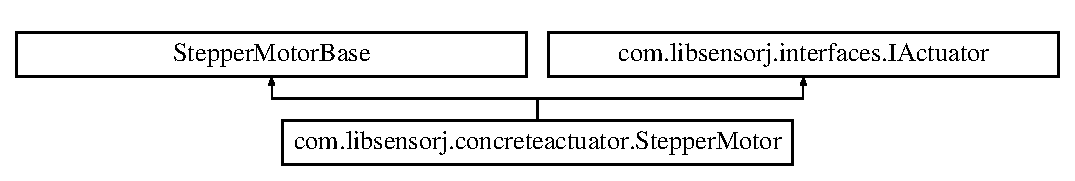
\includegraphics[height=1.985816cm]{classcom_1_1libsensorj_1_1concreteactuator_1_1StepperMotor}
\end{center}
\end{figure}
\subsection*{Classes}
\begin{DoxyCompactItemize}
\item 
class \hyperlink{classcom_1_1libsensorj_1_1concreteactuator_1_1StepperMotor_1_1GpioStepperMotorControl}{Gpio\+Stepper\+Motor\+Control}
\end{DoxyCompactItemize}
\subsection*{Public Member Functions}
\begin{DoxyCompactItemize}
\item 
\hyperlink{classcom_1_1libsensorj_1_1concreteactuator_1_1StepperMotor_a8b5f85a0849fd8de39b415e5cb2903ba}{Stepper\+Motor} (Gpio\+Pin\+Digital\+Output \hyperlink{classcom_1_1libsensorj_1_1concreteactuator_1_1StepperMotor_aefca907f907fd398b7bcdd902e04b928}{pins}\mbox{[}$\,$\mbox{]}, Pin\+State \hyperlink{classcom_1_1libsensorj_1_1concreteactuator_1_1StepperMotor_abcf0537132ae7308214b40125aaeef27}{on\+State}, Pin\+State \hyperlink{classcom_1_1libsensorj_1_1concreteactuator_1_1StepperMotor_a44204d0df9f310e95185bea229c1d23d}{off\+State})
\item 
\hyperlink{classcom_1_1libsensorj_1_1concreteactuator_1_1StepperMotor_a9ac4472f2583dd20460992528a0ca370}{Stepper\+Motor} (Gpio\+Pin\+Digital\+Output \hyperlink{classcom_1_1libsensorj_1_1concreteactuator_1_1StepperMotor_aefca907f907fd398b7bcdd902e04b928}{pins}\mbox{[}$\,$\mbox{]})
\item 
Motor\+State \hyperlink{classcom_1_1libsensorj_1_1concreteactuator_1_1StepperMotor_a589071fa722a01fd7baf7a0133038c74}{get\+State} ()
\item 
void \hyperlink{classcom_1_1libsensorj_1_1concreteactuator_1_1StepperMotor_a683524a2de1c7e967bc89486f9b9164b}{set\+State} (Motor\+State state)
\item 
void \hyperlink{classcom_1_1libsensorj_1_1concreteactuator_1_1StepperMotor_a957195aa23742bd32033d58437e71835}{step} (long steps)
\end{DoxyCompactItemize}
\subsection*{Private Member Functions}
\begin{DoxyCompactItemize}
\item 
void \hyperlink{classcom_1_1libsensorj_1_1concreteactuator_1_1StepperMotor_a063d16fae6c8b67b14efd441a05dbfd6}{motor\+Stop} ()
\item 
void \hyperlink{classcom_1_1libsensorj_1_1concreteactuator_1_1StepperMotor_a8e8e397c042af5e2b00f909de199acd1}{motor\+Start} (Motor\+State state)
\item 
void \hyperlink{classcom_1_1libsensorj_1_1concreteactuator_1_1StepperMotor_a70da2be5b98bdcd51b1098cbef0525f1}{do\+Step} (boolean forward)
\end{DoxyCompactItemize}
\subsection*{Private Attributes}
\begin{DoxyCompactItemize}
\item 
Gpio\+Pin\+Digital\+Output \hyperlink{classcom_1_1libsensorj_1_1concreteactuator_1_1StepperMotor_aefca907f907fd398b7bcdd902e04b928}{pins} \mbox{[}$\,$\mbox{]}
\item 
Pin\+State \hyperlink{classcom_1_1libsensorj_1_1concreteactuator_1_1StepperMotor_abcf0537132ae7308214b40125aaeef27}{on\+State} = Pin\+State.\+H\+I\+G\+H
\item 
Pin\+State \hyperlink{classcom_1_1libsensorj_1_1concreteactuator_1_1StepperMotor_a44204d0df9f310e95185bea229c1d23d}{off\+State} = Pin\+State.\+L\+O\+W
\item 
Motor\+State \hyperlink{classcom_1_1libsensorj_1_1concreteactuator_1_1StepperMotor_a89b1f9ca70656dedab935870972acf79}{current\+State} = Motor\+State.\+S\+T\+O\+P
\item 
\hyperlink{classcom_1_1libsensorj_1_1concreteactuator_1_1StepperMotor_1_1GpioStepperMotorControl}{Gpio\+Stepper\+Motor\+Control} \hyperlink{classcom_1_1libsensorj_1_1concreteactuator_1_1StepperMotor_a3fbdbefa640e24fa09c78962c56aabef}{control\+Thread} = new \hyperlink{classcom_1_1libsensorj_1_1concreteactuator_1_1StepperMotor_1_1GpioStepperMotorControl}{Gpio\+Stepper\+Motor\+Control}()
\item 
int \hyperlink{classcom_1_1libsensorj_1_1concreteactuator_1_1StepperMotor_adc7f82436f61b2a32539f5af34b1c681}{sequence\+Index} = 0
\end{DoxyCompactItemize}


\subsection{Constructor \& Destructor Documentation}
\hypertarget{classcom_1_1libsensorj_1_1concreteactuator_1_1StepperMotor_a8b5f85a0849fd8de39b415e5cb2903ba}{}\index{com\+::libsensorj\+::concreteactuator\+::\+Stepper\+Motor@{com\+::libsensorj\+::concreteactuator\+::\+Stepper\+Motor}!Stepper\+Motor@{Stepper\+Motor}}
\index{Stepper\+Motor@{Stepper\+Motor}!com\+::libsensorj\+::concreteactuator\+::\+Stepper\+Motor@{com\+::libsensorj\+::concreteactuator\+::\+Stepper\+Motor}}
\subsubsection[{Stepper\+Motor}]{\setlength{\rightskip}{0pt plus 5cm}com.\+libsensorj.\+concreteactuator.\+Stepper\+Motor.\+Stepper\+Motor (
\begin{DoxyParamCaption}
\item[{Gpio\+Pin\+Digital\+Output}]{pins\mbox{[}$\,$\mbox{]}, }
\item[{Pin\+State}]{on\+State, }
\item[{Pin\+State}]{off\+State}
\end{DoxyParamCaption}
)}\label{classcom_1_1libsensorj_1_1concreteactuator_1_1StepperMotor_a8b5f85a0849fd8de39b415e5cb2903ba}
using this constructor requires that the consumer define the S\+T\+E\+P O\+N and S\+T\+E\+P O\+F\+F pin states


\begin{DoxyParams}{Parameters}
{\em pins} & G\+P\+I\+O digital output pins for each controller in the stepper motor \\
\hline
{\em on\+State} & pin state to set when M\+O\+T\+O\+R S\+T\+E\+P is O\+N \\
\hline
{\em off\+State} & pin state to set when M\+O\+T\+O\+R S\+T\+E\+P is O\+F\+F \\
\hline
\end{DoxyParams}
\hypertarget{classcom_1_1libsensorj_1_1concreteactuator_1_1StepperMotor_a9ac4472f2583dd20460992528a0ca370}{}\index{com\+::libsensorj\+::concreteactuator\+::\+Stepper\+Motor@{com\+::libsensorj\+::concreteactuator\+::\+Stepper\+Motor}!Stepper\+Motor@{Stepper\+Motor}}
\index{Stepper\+Motor@{Stepper\+Motor}!com\+::libsensorj\+::concreteactuator\+::\+Stepper\+Motor@{com\+::libsensorj\+::concreteactuator\+::\+Stepper\+Motor}}
\subsubsection[{Stepper\+Motor}]{\setlength{\rightskip}{0pt plus 5cm}com.\+libsensorj.\+concreteactuator.\+Stepper\+Motor.\+Stepper\+Motor (
\begin{DoxyParamCaption}
\item[{Gpio\+Pin\+Digital\+Output}]{pins\mbox{[}$\,$\mbox{]}}
\end{DoxyParamCaption}
)}\label{classcom_1_1libsensorj_1_1concreteactuator_1_1StepperMotor_a9ac4472f2583dd20460992528a0ca370}
default constructor; using this constructor assumes that\+: (1) a pin state of H\+I\+G\+H is M\+O\+T\+O\+R S\+T\+E\+P O\+N (2) a pin state of L\+O\+W is M\+O\+T\+O\+R S\+T\+E\+P O\+F\+F


\begin{DoxyParams}{Parameters}
{\em pins} & G\+P\+I\+O digital output pins for each controller in the stepper motor \\
\hline
\end{DoxyParams}


\subsection{Member Function Documentation}
\hypertarget{classcom_1_1libsensorj_1_1concreteactuator_1_1StepperMotor_a70da2be5b98bdcd51b1098cbef0525f1}{}\index{com\+::libsensorj\+::concreteactuator\+::\+Stepper\+Motor@{com\+::libsensorj\+::concreteactuator\+::\+Stepper\+Motor}!do\+Step@{do\+Step}}
\index{do\+Step@{do\+Step}!com\+::libsensorj\+::concreteactuator\+::\+Stepper\+Motor@{com\+::libsensorj\+::concreteactuator\+::\+Stepper\+Motor}}
\subsubsection[{do\+Step}]{\setlength{\rightskip}{0pt plus 5cm}void com.\+libsensorj.\+concreteactuator.\+Stepper\+Motor.\+do\+Step (
\begin{DoxyParamCaption}
\item[{boolean}]{forward}
\end{DoxyParamCaption}
)\hspace{0.3cm}{\ttfamily [private]}}\label{classcom_1_1libsensorj_1_1concreteactuator_1_1StepperMotor_a70da2be5b98bdcd51b1098cbef0525f1}
this method performs the calculations and work to control the G\+P\+I\+O pins to move the stepper motor forward or reverse


\begin{DoxyParams}{Parameters}
{\em forward} & \\
\hline
\end{DoxyParams}
\hypertarget{classcom_1_1libsensorj_1_1concreteactuator_1_1StepperMotor_a589071fa722a01fd7baf7a0133038c74}{}\index{com\+::libsensorj\+::concreteactuator\+::\+Stepper\+Motor@{com\+::libsensorj\+::concreteactuator\+::\+Stepper\+Motor}!get\+State@{get\+State}}
\index{get\+State@{get\+State}!com\+::libsensorj\+::concreteactuator\+::\+Stepper\+Motor@{com\+::libsensorj\+::concreteactuator\+::\+Stepper\+Motor}}
\subsubsection[{get\+State}]{\setlength{\rightskip}{0pt plus 5cm}Motor\+State com.\+libsensorj.\+concreteactuator.\+Stepper\+Motor.\+get\+State (
\begin{DoxyParamCaption}
{}
\end{DoxyParamCaption}
)}\label{classcom_1_1libsensorj_1_1concreteactuator_1_1StepperMotor_a589071fa722a01fd7baf7a0133038c74}
Return the current motor state

\begin{DoxyReturn}{Returns}
Motor\+State 
\end{DoxyReturn}
\hypertarget{classcom_1_1libsensorj_1_1concreteactuator_1_1StepperMotor_a8e8e397c042af5e2b00f909de199acd1}{}\index{com\+::libsensorj\+::concreteactuator\+::\+Stepper\+Motor@{com\+::libsensorj\+::concreteactuator\+::\+Stepper\+Motor}!motor\+Start@{motor\+Start}}
\index{motor\+Start@{motor\+Start}!com\+::libsensorj\+::concreteactuator\+::\+Stepper\+Motor@{com\+::libsensorj\+::concreteactuator\+::\+Stepper\+Motor}}
\subsubsection[{motor\+Start}]{\setlength{\rightskip}{0pt plus 5cm}void com.\+libsensorj.\+concreteactuator.\+Stepper\+Motor.\+motor\+Start (
\begin{DoxyParamCaption}
\item[{Motor\+State}]{state}
\end{DoxyParamCaption}
)\hspace{0.3cm}{\ttfamily [private]}}\label{classcom_1_1libsensorj_1_1concreteactuator_1_1StepperMotor_a8e8e397c042af5e2b00f909de199acd1}
\hypertarget{classcom_1_1libsensorj_1_1concreteactuator_1_1StepperMotor_a063d16fae6c8b67b14efd441a05dbfd6}{}\index{com\+::libsensorj\+::concreteactuator\+::\+Stepper\+Motor@{com\+::libsensorj\+::concreteactuator\+::\+Stepper\+Motor}!motor\+Stop@{motor\+Stop}}
\index{motor\+Stop@{motor\+Stop}!com\+::libsensorj\+::concreteactuator\+::\+Stepper\+Motor@{com\+::libsensorj\+::concreteactuator\+::\+Stepper\+Motor}}
\subsubsection[{motor\+Stop}]{\setlength{\rightskip}{0pt plus 5cm}void com.\+libsensorj.\+concreteactuator.\+Stepper\+Motor.\+motor\+Stop (
\begin{DoxyParamCaption}
{}
\end{DoxyParamCaption}
)\hspace{0.3cm}{\ttfamily [private]}}\label{classcom_1_1libsensorj_1_1concreteactuator_1_1StepperMotor_a063d16fae6c8b67b14efd441a05dbfd6}
\hypertarget{classcom_1_1libsensorj_1_1concreteactuator_1_1StepperMotor_a683524a2de1c7e967bc89486f9b9164b}{}\index{com\+::libsensorj\+::concreteactuator\+::\+Stepper\+Motor@{com\+::libsensorj\+::concreteactuator\+::\+Stepper\+Motor}!set\+State@{set\+State}}
\index{set\+State@{set\+State}!com\+::libsensorj\+::concreteactuator\+::\+Stepper\+Motor@{com\+::libsensorj\+::concreteactuator\+::\+Stepper\+Motor}}
\subsubsection[{set\+State}]{\setlength{\rightskip}{0pt plus 5cm}void com.\+libsensorj.\+concreteactuator.\+Stepper\+Motor.\+set\+State (
\begin{DoxyParamCaption}
\item[{Motor\+State}]{state}
\end{DoxyParamCaption}
)}\label{classcom_1_1libsensorj_1_1concreteactuator_1_1StepperMotor_a683524a2de1c7e967bc89486f9b9164b}
change the current stepper motor state


\begin{DoxyParams}{Parameters}
{\em state} & new motor state to apply \\
\hline
\end{DoxyParams}
\hypertarget{classcom_1_1libsensorj_1_1concreteactuator_1_1StepperMotor_a957195aa23742bd32033d58437e71835}{}\index{com\+::libsensorj\+::concreteactuator\+::\+Stepper\+Motor@{com\+::libsensorj\+::concreteactuator\+::\+Stepper\+Motor}!step@{step}}
\index{step@{step}!com\+::libsensorj\+::concreteactuator\+::\+Stepper\+Motor@{com\+::libsensorj\+::concreteactuator\+::\+Stepper\+Motor}}
\subsubsection[{step}]{\setlength{\rightskip}{0pt plus 5cm}void com.\+libsensorj.\+concreteactuator.\+Stepper\+Motor.\+step (
\begin{DoxyParamCaption}
\item[{long}]{steps}
\end{DoxyParamCaption}
)}\label{classcom_1_1libsensorj_1_1concreteactuator_1_1StepperMotor_a957195aa23742bd32033d58437e71835}


\subsection{Member Data Documentation}
\hypertarget{classcom_1_1libsensorj_1_1concreteactuator_1_1StepperMotor_a3fbdbefa640e24fa09c78962c56aabef}{}\index{com\+::libsensorj\+::concreteactuator\+::\+Stepper\+Motor@{com\+::libsensorj\+::concreteactuator\+::\+Stepper\+Motor}!control\+Thread@{control\+Thread}}
\index{control\+Thread@{control\+Thread}!com\+::libsensorj\+::concreteactuator\+::\+Stepper\+Motor@{com\+::libsensorj\+::concreteactuator\+::\+Stepper\+Motor}}
\subsubsection[{control\+Thread}]{\setlength{\rightskip}{0pt plus 5cm}{\bf Gpio\+Stepper\+Motor\+Control} com.\+libsensorj.\+concreteactuator.\+Stepper\+Motor.\+control\+Thread = new {\bf Gpio\+Stepper\+Motor\+Control}()\hspace{0.3cm}{\ttfamily [private]}}\label{classcom_1_1libsensorj_1_1concreteactuator_1_1StepperMotor_a3fbdbefa640e24fa09c78962c56aabef}
\hypertarget{classcom_1_1libsensorj_1_1concreteactuator_1_1StepperMotor_a89b1f9ca70656dedab935870972acf79}{}\index{com\+::libsensorj\+::concreteactuator\+::\+Stepper\+Motor@{com\+::libsensorj\+::concreteactuator\+::\+Stepper\+Motor}!current\+State@{current\+State}}
\index{current\+State@{current\+State}!com\+::libsensorj\+::concreteactuator\+::\+Stepper\+Motor@{com\+::libsensorj\+::concreteactuator\+::\+Stepper\+Motor}}
\subsubsection[{current\+State}]{\setlength{\rightskip}{0pt plus 5cm}Motor\+State com.\+libsensorj.\+concreteactuator.\+Stepper\+Motor.\+current\+State = Motor\+State.\+S\+T\+O\+P\hspace{0.3cm}{\ttfamily [private]}}\label{classcom_1_1libsensorj_1_1concreteactuator_1_1StepperMotor_a89b1f9ca70656dedab935870972acf79}
\hypertarget{classcom_1_1libsensorj_1_1concreteactuator_1_1StepperMotor_a44204d0df9f310e95185bea229c1d23d}{}\index{com\+::libsensorj\+::concreteactuator\+::\+Stepper\+Motor@{com\+::libsensorj\+::concreteactuator\+::\+Stepper\+Motor}!off\+State@{off\+State}}
\index{off\+State@{off\+State}!com\+::libsensorj\+::concreteactuator\+::\+Stepper\+Motor@{com\+::libsensorj\+::concreteactuator\+::\+Stepper\+Motor}}
\subsubsection[{off\+State}]{\setlength{\rightskip}{0pt plus 5cm}Pin\+State com.\+libsensorj.\+concreteactuator.\+Stepper\+Motor.\+off\+State = Pin\+State.\+L\+O\+W\hspace{0.3cm}{\ttfamily [private]}}\label{classcom_1_1libsensorj_1_1concreteactuator_1_1StepperMotor_a44204d0df9f310e95185bea229c1d23d}
\hypertarget{classcom_1_1libsensorj_1_1concreteactuator_1_1StepperMotor_abcf0537132ae7308214b40125aaeef27}{}\index{com\+::libsensorj\+::concreteactuator\+::\+Stepper\+Motor@{com\+::libsensorj\+::concreteactuator\+::\+Stepper\+Motor}!on\+State@{on\+State}}
\index{on\+State@{on\+State}!com\+::libsensorj\+::concreteactuator\+::\+Stepper\+Motor@{com\+::libsensorj\+::concreteactuator\+::\+Stepper\+Motor}}
\subsubsection[{on\+State}]{\setlength{\rightskip}{0pt plus 5cm}Pin\+State com.\+libsensorj.\+concreteactuator.\+Stepper\+Motor.\+on\+State = Pin\+State.\+H\+I\+G\+H\hspace{0.3cm}{\ttfamily [private]}}\label{classcom_1_1libsensorj_1_1concreteactuator_1_1StepperMotor_abcf0537132ae7308214b40125aaeef27}
\hypertarget{classcom_1_1libsensorj_1_1concreteactuator_1_1StepperMotor_aefca907f907fd398b7bcdd902e04b928}{}\index{com\+::libsensorj\+::concreteactuator\+::\+Stepper\+Motor@{com\+::libsensorj\+::concreteactuator\+::\+Stepper\+Motor}!pins@{pins}}
\index{pins@{pins}!com\+::libsensorj\+::concreteactuator\+::\+Stepper\+Motor@{com\+::libsensorj\+::concreteactuator\+::\+Stepper\+Motor}}
\subsubsection[{pins}]{\setlength{\rightskip}{0pt plus 5cm}Gpio\+Pin\+Digital\+Output com.\+libsensorj.\+concreteactuator.\+Stepper\+Motor.\+pins\mbox{[}$\,$\mbox{]}\hspace{0.3cm}{\ttfamily [private]}}\label{classcom_1_1libsensorj_1_1concreteactuator_1_1StepperMotor_aefca907f907fd398b7bcdd902e04b928}
\hypertarget{classcom_1_1libsensorj_1_1concreteactuator_1_1StepperMotor_adc7f82436f61b2a32539f5af34b1c681}{}\index{com\+::libsensorj\+::concreteactuator\+::\+Stepper\+Motor@{com\+::libsensorj\+::concreteactuator\+::\+Stepper\+Motor}!sequence\+Index@{sequence\+Index}}
\index{sequence\+Index@{sequence\+Index}!com\+::libsensorj\+::concreteactuator\+::\+Stepper\+Motor@{com\+::libsensorj\+::concreteactuator\+::\+Stepper\+Motor}}
\subsubsection[{sequence\+Index}]{\setlength{\rightskip}{0pt plus 5cm}int com.\+libsensorj.\+concreteactuator.\+Stepper\+Motor.\+sequence\+Index = 0\hspace{0.3cm}{\ttfamily [private]}}\label{classcom_1_1libsensorj_1_1concreteactuator_1_1StepperMotor_adc7f82436f61b2a32539f5af34b1c681}


The documentation for this class was generated from the following file\+:\begin{DoxyCompactItemize}
\item 
main/java/com/libsensorj/concreteactuator/\hyperlink{StepperMotor_8java}{Stepper\+Motor.\+java}\end{DoxyCompactItemize}

\hypertarget{classcom_1_1libsensorj_1_1examples_1_1StepperMotorExample}{}\section{com.\+libsensorj.\+examples.\+Stepper\+Motor\+Example Class Reference}
\label{classcom_1_1libsensorj_1_1examples_1_1StepperMotorExample}\index{com.\+libsensorj.\+examples.\+Stepper\+Motor\+Example@{com.\+libsensorj.\+examples.\+Stepper\+Motor\+Example}}
\subsection*{Static Public Member Functions}
\begin{DoxyCompactItemize}
\item 
static void \hyperlink{classcom_1_1libsensorj_1_1examples_1_1StepperMotorExample_af5663da7f40076dadce70f061adad200}{main} (String\mbox{[}$\,$\mbox{]} args)  throws Interrupted\+Exception 
\end{DoxyCompactItemize}


\subsection{Member Function Documentation}
\hypertarget{classcom_1_1libsensorj_1_1examples_1_1StepperMotorExample_af5663da7f40076dadce70f061adad200}{}\index{com\+::libsensorj\+::examples\+::\+Stepper\+Motor\+Example@{com\+::libsensorj\+::examples\+::\+Stepper\+Motor\+Example}!main@{main}}
\index{main@{main}!com\+::libsensorj\+::examples\+::\+Stepper\+Motor\+Example@{com\+::libsensorj\+::examples\+::\+Stepper\+Motor\+Example}}
\subsubsection[{main}]{\setlength{\rightskip}{0pt plus 5cm}static void com.\+libsensorj.\+examples.\+Stepper\+Motor\+Example.\+main (
\begin{DoxyParamCaption}
\item[{String\mbox{[}$\,$\mbox{]}}]{args}
\end{DoxyParamCaption}
) throws Interrupted\+Exception\hspace{0.3cm}{\ttfamily [static]}}\label{classcom_1_1libsensorj_1_1examples_1_1StepperMotorExample_af5663da7f40076dadce70f061adad200}


The documentation for this class was generated from the following file\+:\begin{DoxyCompactItemize}
\item 
main/java/com/libsensorj/examples/\hyperlink{StepperMotorExample_8java}{Stepper\+Motor\+Example.\+java}\end{DoxyCompactItemize}

\hypertarget{classcom_1_1libsensorj_1_1concreteevent_1_1TemperatureEvent}{}\section{com.\+libsensorj.\+concreteevent.\+Temperature\+Event Class Reference}
\label{classcom_1_1libsensorj_1_1concreteevent_1_1TemperatureEvent}\index{com.\+libsensorj.\+concreteevent.\+Temperature\+Event@{com.\+libsensorj.\+concreteevent.\+Temperature\+Event}}
Inheritance diagram for com.\+libsensorj.\+concreteevent.\+Temperature\+Event\+:\begin{figure}[H]
\begin{center}
\leavevmode
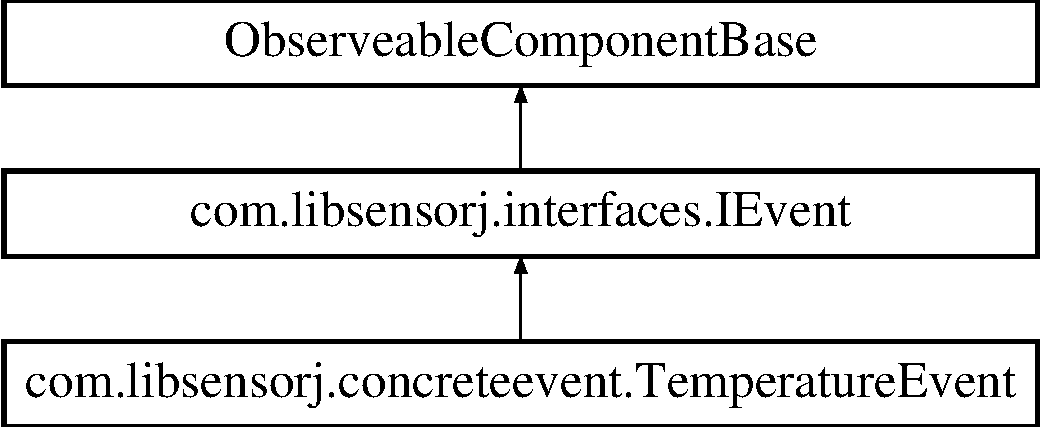
\includegraphics[height=3.000000cm]{classcom_1_1libsensorj_1_1concreteevent_1_1TemperatureEvent}
\end{center}
\end{figure}
\subsection*{Public Member Functions}
\begin{DoxyCompactItemize}
\item 
void \hyperlink{classcom_1_1libsensorj_1_1concreteevent_1_1TemperatureEvent_ad3499315aef403dfde60cf7d9a42c8cf}{attach} (\hyperlink{classcom_1_1libsensorj_1_1model_1_1Observer}{Observer} obsever)
\item 
void \hyperlink{classcom_1_1libsensorj_1_1concreteevent_1_1TemperatureEvent_a7332f144af23c349f39dd714de9c07b9}{detach} (\hyperlink{classcom_1_1libsensorj_1_1model_1_1Observer}{Observer} obsever)
\item 
void \hyperlink{classcom_1_1libsensorj_1_1concreteevent_1_1TemperatureEvent_ac0fe5a9964739808ece4fc9f2562dca5}{trigger} ()
\end{DoxyCompactItemize}


\subsection{Detailed Description}
The Class \hyperlink{classcom_1_1libsensorj_1_1concreteevent_1_1TemperatureEvent}{Temperature\+Event}. 

\subsection{Member Function Documentation}
\hypertarget{classcom_1_1libsensorj_1_1concreteevent_1_1TemperatureEvent_ad3499315aef403dfde60cf7d9a42c8cf}{}\index{com\+::libsensorj\+::concreteevent\+::\+Temperature\+Event@{com\+::libsensorj\+::concreteevent\+::\+Temperature\+Event}!attach@{attach}}
\index{attach@{attach}!com\+::libsensorj\+::concreteevent\+::\+Temperature\+Event@{com\+::libsensorj\+::concreteevent\+::\+Temperature\+Event}}
\subsubsection[{attach}]{\setlength{\rightskip}{0pt plus 5cm}void com.\+libsensorj.\+concreteevent.\+Temperature\+Event.\+attach (
\begin{DoxyParamCaption}
\item[{{\bf Observer}}]{obsever}
\end{DoxyParamCaption}
)}\label{classcom_1_1libsensorj_1_1concreteevent_1_1TemperatureEvent_ad3499315aef403dfde60cf7d9a42c8cf}
\hypertarget{classcom_1_1libsensorj_1_1concreteevent_1_1TemperatureEvent_a7332f144af23c349f39dd714de9c07b9}{}\index{com\+::libsensorj\+::concreteevent\+::\+Temperature\+Event@{com\+::libsensorj\+::concreteevent\+::\+Temperature\+Event}!detach@{detach}}
\index{detach@{detach}!com\+::libsensorj\+::concreteevent\+::\+Temperature\+Event@{com\+::libsensorj\+::concreteevent\+::\+Temperature\+Event}}
\subsubsection[{detach}]{\setlength{\rightskip}{0pt plus 5cm}void com.\+libsensorj.\+concreteevent.\+Temperature\+Event.\+detach (
\begin{DoxyParamCaption}
\item[{{\bf Observer}}]{obsever}
\end{DoxyParamCaption}
)}\label{classcom_1_1libsensorj_1_1concreteevent_1_1TemperatureEvent_a7332f144af23c349f39dd714de9c07b9}
\hypertarget{classcom_1_1libsensorj_1_1concreteevent_1_1TemperatureEvent_ac0fe5a9964739808ece4fc9f2562dca5}{}\index{com\+::libsensorj\+::concreteevent\+::\+Temperature\+Event@{com\+::libsensorj\+::concreteevent\+::\+Temperature\+Event}!trigger@{trigger}}
\index{trigger@{trigger}!com\+::libsensorj\+::concreteevent\+::\+Temperature\+Event@{com\+::libsensorj\+::concreteevent\+::\+Temperature\+Event}}
\subsubsection[{trigger}]{\setlength{\rightskip}{0pt plus 5cm}void com.\+libsensorj.\+concreteevent.\+Temperature\+Event.\+trigger (
\begin{DoxyParamCaption}
{}
\end{DoxyParamCaption}
)}\label{classcom_1_1libsensorj_1_1concreteevent_1_1TemperatureEvent_ac0fe5a9964739808ece4fc9f2562dca5}


The documentation for this class was generated from the following file\+:\begin{DoxyCompactItemize}
\item 
main/java/com/libsensorj/concreteevent/\hyperlink{TemperatureEvent_8java}{Temperature\+Event.\+java}\end{DoxyCompactItemize}

\hypertarget{classcom_1_1libsensorj_1_1concretefactory_1_1TemperatureSensorFactory}{}\section{com.\+libsensorj.\+concretefactory.\+Temperature\+Sensor\+Factory Class Reference}
\label{classcom_1_1libsensorj_1_1concretefactory_1_1TemperatureSensorFactory}\index{com.\+libsensorj.\+concretefactory.\+Temperature\+Sensor\+Factory@{com.\+libsensorj.\+concretefactory.\+Temperature\+Sensor\+Factory}}
Inheritance diagram for com.\+libsensorj.\+concretefactory.\+Temperature\+Sensor\+Factory\+:\begin{figure}[H]
\begin{center}
\leavevmode
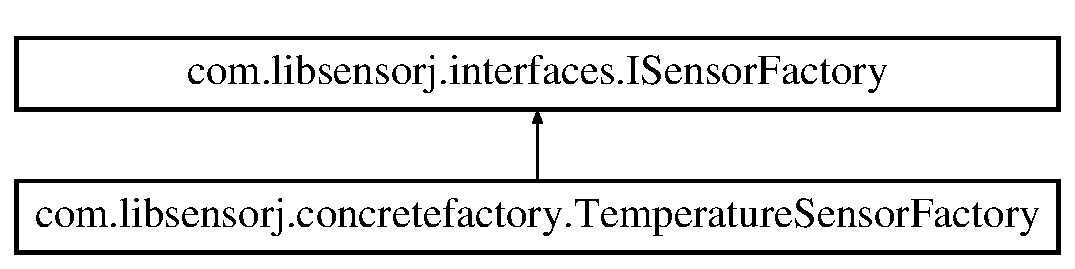
\includegraphics[height=2.000000cm]{classcom_1_1libsensorj_1_1concretefactory_1_1TemperatureSensorFactory}
\end{center}
\end{figure}
\subsection*{Public Member Functions}
\begin{DoxyCompactItemize}
\item 
\hyperlink{interfacecom_1_1libsensorj_1_1interfaces_1_1ISensor}{I\+Sensor} \hyperlink{classcom_1_1libsensorj_1_1concretefactory_1_1TemperatureSensorFactory_aeba8598ebe5c182154f63e0c94abdd70}{create\+Sensor} ()
\item 
\hyperlink{interfacecom_1_1libsensorj_1_1interfaces_1_1IEvent}{I\+Event} \hyperlink{classcom_1_1libsensorj_1_1concretefactory_1_1TemperatureSensorFactory_adb3d5716b5e55f4fc037c0a95ec99688}{create\+Event} ()
\end{DoxyCompactItemize}


\subsection{Member Function Documentation}
\hypertarget{classcom_1_1libsensorj_1_1concretefactory_1_1TemperatureSensorFactory_adb3d5716b5e55f4fc037c0a95ec99688}{}\index{com\+::libsensorj\+::concretefactory\+::\+Temperature\+Sensor\+Factory@{com\+::libsensorj\+::concretefactory\+::\+Temperature\+Sensor\+Factory}!create\+Event@{create\+Event}}
\index{create\+Event@{create\+Event}!com\+::libsensorj\+::concretefactory\+::\+Temperature\+Sensor\+Factory@{com\+::libsensorj\+::concretefactory\+::\+Temperature\+Sensor\+Factory}}
\subsubsection[{create\+Event}]{\setlength{\rightskip}{0pt plus 5cm}{\bf I\+Event} com.\+libsensorj.\+concretefactory.\+Temperature\+Sensor\+Factory.\+create\+Event (
\begin{DoxyParamCaption}
{}
\end{DoxyParamCaption}
)}\label{classcom_1_1libsensorj_1_1concretefactory_1_1TemperatureSensorFactory_adb3d5716b5e55f4fc037c0a95ec99688}


Implements \hyperlink{interfacecom_1_1libsensorj_1_1interfaces_1_1ISensorFactory_a2b074d01287a4e64677097255ba9e768}{com.\+libsensorj.\+interfaces.\+I\+Sensor\+Factory}.

\hypertarget{classcom_1_1libsensorj_1_1concretefactory_1_1TemperatureSensorFactory_aeba8598ebe5c182154f63e0c94abdd70}{}\index{com\+::libsensorj\+::concretefactory\+::\+Temperature\+Sensor\+Factory@{com\+::libsensorj\+::concretefactory\+::\+Temperature\+Sensor\+Factory}!create\+Sensor@{create\+Sensor}}
\index{create\+Sensor@{create\+Sensor}!com\+::libsensorj\+::concretefactory\+::\+Temperature\+Sensor\+Factory@{com\+::libsensorj\+::concretefactory\+::\+Temperature\+Sensor\+Factory}}
\subsubsection[{create\+Sensor}]{\setlength{\rightskip}{0pt plus 5cm}{\bf I\+Sensor} com.\+libsensorj.\+concretefactory.\+Temperature\+Sensor\+Factory.\+create\+Sensor (
\begin{DoxyParamCaption}
{}
\end{DoxyParamCaption}
)}\label{classcom_1_1libsensorj_1_1concretefactory_1_1TemperatureSensorFactory_aeba8598ebe5c182154f63e0c94abdd70}


Implements \hyperlink{interfacecom_1_1libsensorj_1_1interfaces_1_1ISensorFactory_ac14c6d566c37c6a79c6db1e85634f25d}{com.\+libsensorj.\+interfaces.\+I\+Sensor\+Factory}.



The documentation for this class was generated from the following file\+:\begin{DoxyCompactItemize}
\item 
main/java/com/libsensorj/concretefactory/\hyperlink{TemperatureSensorFactory_8java}{Temperature\+Sensor\+Factory.\+java}\end{DoxyCompactItemize}

\hypertarget{classcom_1_1libsensorj_1_1concretefactory_1_1test_1_1TemperatureSensorFactoryTests}{}\section{com.\+libsensorj.\+concretefactory.\+test.\+Temperature\+Sensor\+Factory\+Tests Class Reference}
\label{classcom_1_1libsensorj_1_1concretefactory_1_1test_1_1TemperatureSensorFactoryTests}\index{com.\+libsensorj.\+concretefactory.\+test.\+Temperature\+Sensor\+Factory\+Tests@{com.\+libsensorj.\+concretefactory.\+test.\+Temperature\+Sensor\+Factory\+Tests}}
\subsection*{Public Member Functions}
\begin{DoxyCompactItemize}
\item 
void \hyperlink{classcom_1_1libsensorj_1_1concretefactory_1_1test_1_1TemperatureSensorFactoryTests_aadff44b1575570522d980e5471eac596}{test} ()
\end{DoxyCompactItemize}


\subsection{Detailed Description}
The Class \hyperlink{classcom_1_1libsensorj_1_1concretefactory_1_1test_1_1TemperatureSensorFactoryTests}{Temperature\+Sensor\+Factory\+Tests}. 

\subsection{Member Function Documentation}
\hypertarget{classcom_1_1libsensorj_1_1concretefactory_1_1test_1_1TemperatureSensorFactoryTests_aadff44b1575570522d980e5471eac596}{}\index{com\+::libsensorj\+::concretefactory\+::test\+::\+Temperature\+Sensor\+Factory\+Tests@{com\+::libsensorj\+::concretefactory\+::test\+::\+Temperature\+Sensor\+Factory\+Tests}!test@{test}}
\index{test@{test}!com\+::libsensorj\+::concretefactory\+::test\+::\+Temperature\+Sensor\+Factory\+Tests@{com\+::libsensorj\+::concretefactory\+::test\+::\+Temperature\+Sensor\+Factory\+Tests}}
\subsubsection[{test}]{\setlength{\rightskip}{0pt plus 5cm}void com.\+libsensorj.\+concretefactory.\+test.\+Temperature\+Sensor\+Factory\+Tests.\+test (
\begin{DoxyParamCaption}
{}
\end{DoxyParamCaption}
)}\label{classcom_1_1libsensorj_1_1concretefactory_1_1test_1_1TemperatureSensorFactoryTests_aadff44b1575570522d980e5471eac596}
Test. 

The documentation for this class was generated from the following file\+:\begin{DoxyCompactItemize}
\item 
test/java/com/libsensorj/concretefactory/test/\hyperlink{TemperatureSensorFactoryTests_8java}{Temperature\+Sensor\+Factory\+Tests.\+java}\end{DoxyCompactItemize}

\hypertarget{classcom_1_1libsensorj_1_1concretesensor_1_1UltrasonicHcsr04}{}\section{com.\+libsensorj.\+concretesensor.\+Ultrasonic\+Hcsr04 Class Reference}
\label{classcom_1_1libsensorj_1_1concretesensor_1_1UltrasonicHcsr04}\index{com.\+libsensorj.\+concretesensor.\+Ultrasonic\+Hcsr04@{com.\+libsensorj.\+concretesensor.\+Ultrasonic\+Hcsr04}}
Inheritance diagram for com.\+libsensorj.\+concretesensor.\+Ultrasonic\+Hcsr04\+:\begin{figure}[H]
\begin{center}
\leavevmode
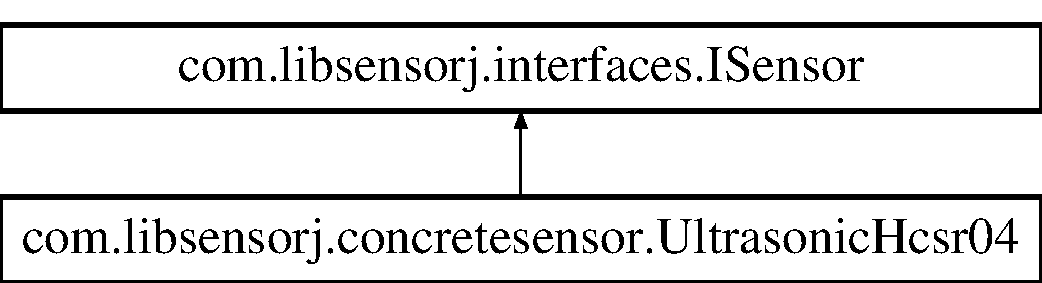
\includegraphics[height=2.000000cm]{classcom_1_1libsensorj_1_1concretesensor_1_1UltrasonicHcsr04}
\end{center}
\end{figure}
\subsection*{Public Member Functions}
\begin{DoxyCompactItemize}
\item 
\hyperlink{classcom_1_1libsensorj_1_1concretesensor_1_1UltrasonicHcsr04_a7e02068d9acb1b3cf1d15d45afbf377b}{Ultrasonic\+Hcsr04} ()
\item 
\hyperlink{classcom_1_1libsensorj_1_1concretesensor_1_1UltrasonicHcsr04_a14e708bf4eb89a2ceb0037fcb837522c}{Ultrasonic\+Hcsr04} (int \hyperlink{classcom_1_1libsensorj_1_1concretesensor_1_1UltrasonicHcsr04_a13705a8251de22d0f52caa3e17d23376}{trigger}, int \hyperlink{classcom_1_1libsensorj_1_1concretesensor_1_1UltrasonicHcsr04_a3695a560e3157a5e6f7896532d717456}{echo})
\item 
\hyperlink{classcom_1_1libsensorj_1_1concretesensor_1_1UltrasonicHcsr04_ae00a91eaf7e5c08695c50a670698ed5f}{Ultrasonic\+Hcsr04} (Pin \hyperlink{classcom_1_1libsensorj_1_1concretesensor_1_1UltrasonicHcsr04_a13705a8251de22d0f52caa3e17d23376}{trigger}, Pin \hyperlink{classcom_1_1libsensorj_1_1concretesensor_1_1UltrasonicHcsr04_a3695a560e3157a5e6f7896532d717456}{echo})
\item 
void \hyperlink{classcom_1_1libsensorj_1_1concretesensor_1_1UltrasonicHcsr04_a170167614b330d79518647a9a9722b62}{get\+Instance} ()
\item 
double \hyperlink{classcom_1_1libsensorj_1_1concretesensor_1_1UltrasonicHcsr04_aec68f4aadd8faa618025dfa37c89c696}{get\+Range} ()
\end{DoxyCompactItemize}
\subsection*{Private Attributes}
\begin{DoxyCompactItemize}
\item 
double \hyperlink{classcom_1_1libsensorj_1_1concretesensor_1_1UltrasonicHcsr04_aad32f417f9106fa8f3f2e2a7416f033b}{result} = 0
\item 
Gpio\+Pin\+Digital\+Output \hyperlink{classcom_1_1libsensorj_1_1concretesensor_1_1UltrasonicHcsr04_a13705a8251de22d0f52caa3e17d23376}{trigger}
\item 
Gpio\+Pin\+Digital\+Input \hyperlink{classcom_1_1libsensorj_1_1concretesensor_1_1UltrasonicHcsr04_a3695a560e3157a5e6f7896532d717456}{echo}
\end{DoxyCompactItemize}
\subsection*{Static Private Attributes}
\begin{DoxyCompactItemize}
\item 
static final int \hyperlink{classcom_1_1libsensorj_1_1concretesensor_1_1UltrasonicHcsr04_aa04a319fc4ef2ccf8de8a70bf27da2da}{T\+W\+E\+N\+T\+Y} = 20
\item 
static final int \hyperlink{classcom_1_1libsensorj_1_1concretesensor_1_1UltrasonicHcsr04_a7106eaa9f89d876a4749d502232964df}{F\+O\+R\+T\+Y} = 40
\item 
static final int \hyperlink{classcom_1_1libsensorj_1_1concretesensor_1_1UltrasonicHcsr04_a25452283296d3780a7fefbfa20e40a93}{T\+H\+I\+R\+T\+Y\+\_\+\+E\+I\+G\+H\+T} = 38
\item 
static final double \hyperlink{classcom_1_1libsensorj_1_1concretesensor_1_1UltrasonicHcsr04_a0483c4e470b1ab9e1a437fbeec6595e9}{D\+I\+S\+T\+A\+N\+C\+E\+\_\+\+F\+A\+C\+T\+O\+R} = 165.\+7
\item 
static final Logger \hyperlink{classcom_1_1libsensorj_1_1concretesensor_1_1UltrasonicHcsr04_a9a3534d952f2668b69b0888b9e929abb}{L\+O\+G\+G\+E\+R}
\end{DoxyCompactItemize}


\subsection{Detailed Description}
The Class \hyperlink{classcom_1_1libsensorj_1_1concretesensor_1_1UltrasonicHcsr04}{Ultrasonic\+Hcsr04}. 

\subsection{Constructor \& Destructor Documentation}
\hypertarget{classcom_1_1libsensorj_1_1concretesensor_1_1UltrasonicHcsr04_a7e02068d9acb1b3cf1d15d45afbf377b}{}\index{com\+::libsensorj\+::concretesensor\+::\+Ultrasonic\+Hcsr04@{com\+::libsensorj\+::concretesensor\+::\+Ultrasonic\+Hcsr04}!Ultrasonic\+Hcsr04@{Ultrasonic\+Hcsr04}}
\index{Ultrasonic\+Hcsr04@{Ultrasonic\+Hcsr04}!com\+::libsensorj\+::concretesensor\+::\+Ultrasonic\+Hcsr04@{com\+::libsensorj\+::concretesensor\+::\+Ultrasonic\+Hcsr04}}
\subsubsection[{Ultrasonic\+Hcsr04}]{\setlength{\rightskip}{0pt plus 5cm}com.\+libsensorj.\+concretesensor.\+Ultrasonic\+Hcsr04.\+Ultrasonic\+Hcsr04 (
\begin{DoxyParamCaption}
{}
\end{DoxyParamCaption}
)}\label{classcom_1_1libsensorj_1_1concretesensor_1_1UltrasonicHcsr04_a7e02068d9acb1b3cf1d15d45afbf377b}
Instantiates a new ultrasonic hcsr04. \hypertarget{classcom_1_1libsensorj_1_1concretesensor_1_1UltrasonicHcsr04_a14e708bf4eb89a2ceb0037fcb837522c}{}\index{com\+::libsensorj\+::concretesensor\+::\+Ultrasonic\+Hcsr04@{com\+::libsensorj\+::concretesensor\+::\+Ultrasonic\+Hcsr04}!Ultrasonic\+Hcsr04@{Ultrasonic\+Hcsr04}}
\index{Ultrasonic\+Hcsr04@{Ultrasonic\+Hcsr04}!com\+::libsensorj\+::concretesensor\+::\+Ultrasonic\+Hcsr04@{com\+::libsensorj\+::concretesensor\+::\+Ultrasonic\+Hcsr04}}
\subsubsection[{Ultrasonic\+Hcsr04}]{\setlength{\rightskip}{0pt plus 5cm}com.\+libsensorj.\+concretesensor.\+Ultrasonic\+Hcsr04.\+Ultrasonic\+Hcsr04 (
\begin{DoxyParamCaption}
\item[{int}]{trigger, }
\item[{int}]{echo}
\end{DoxyParamCaption}
)}\label{classcom_1_1libsensorj_1_1concretesensor_1_1UltrasonicHcsr04_a14e708bf4eb89a2ceb0037fcb837522c}
Instantiates a new ultrasonic hcsr04.


\begin{DoxyParams}{Parameters}
{\em trigger} & the trigger pin \\
\hline
{\em echo} & the echo pin \\
\hline
\end{DoxyParams}
\hypertarget{classcom_1_1libsensorj_1_1concretesensor_1_1UltrasonicHcsr04_ae00a91eaf7e5c08695c50a670698ed5f}{}\index{com\+::libsensorj\+::concretesensor\+::\+Ultrasonic\+Hcsr04@{com\+::libsensorj\+::concretesensor\+::\+Ultrasonic\+Hcsr04}!Ultrasonic\+Hcsr04@{Ultrasonic\+Hcsr04}}
\index{Ultrasonic\+Hcsr04@{Ultrasonic\+Hcsr04}!com\+::libsensorj\+::concretesensor\+::\+Ultrasonic\+Hcsr04@{com\+::libsensorj\+::concretesensor\+::\+Ultrasonic\+Hcsr04}}
\subsubsection[{Ultrasonic\+Hcsr04}]{\setlength{\rightskip}{0pt plus 5cm}com.\+libsensorj.\+concretesensor.\+Ultrasonic\+Hcsr04.\+Ultrasonic\+Hcsr04 (
\begin{DoxyParamCaption}
\item[{Pin}]{trigger, }
\item[{Pin}]{echo}
\end{DoxyParamCaption}
)}\label{classcom_1_1libsensorj_1_1concretesensor_1_1UltrasonicHcsr04_ae00a91eaf7e5c08695c50a670698ed5f}
Instantiates a new ultrasonic hcsr04.


\begin{DoxyParams}{Parameters}
{\em \+\_\+trigger} & the trigger pin \\
\hline
{\em \+\_\+echo} & the echo pin \\
\hline
\end{DoxyParams}


\subsection{Member Function Documentation}
\hypertarget{classcom_1_1libsensorj_1_1concretesensor_1_1UltrasonicHcsr04_a170167614b330d79518647a9a9722b62}{}\index{com\+::libsensorj\+::concretesensor\+::\+Ultrasonic\+Hcsr04@{com\+::libsensorj\+::concretesensor\+::\+Ultrasonic\+Hcsr04}!get\+Instance@{get\+Instance}}
\index{get\+Instance@{get\+Instance}!com\+::libsensorj\+::concretesensor\+::\+Ultrasonic\+Hcsr04@{com\+::libsensorj\+::concretesensor\+::\+Ultrasonic\+Hcsr04}}
\subsubsection[{get\+Instance}]{\setlength{\rightskip}{0pt plus 5cm}void com.\+libsensorj.\+concretesensor.\+Ultrasonic\+Hcsr04.\+get\+Instance (
\begin{DoxyParamCaption}
{}
\end{DoxyParamCaption}
)}\label{classcom_1_1libsensorj_1_1concretesensor_1_1UltrasonicHcsr04_a170167614b330d79518647a9a9722b62}
Gets the single instance of I\+Sensor.

\begin{DoxyReturn}{Returns}
single instance of I\+Sensor 
\end{DoxyReturn}


Implements \hyperlink{interfacecom_1_1libsensorj_1_1interfaces_1_1ISensor_a3c3db93a33adecde81a528651790f75e}{com.\+libsensorj.\+interfaces.\+I\+Sensor}.

\hypertarget{classcom_1_1libsensorj_1_1concretesensor_1_1UltrasonicHcsr04_aec68f4aadd8faa618025dfa37c89c696}{}\index{com\+::libsensorj\+::concretesensor\+::\+Ultrasonic\+Hcsr04@{com\+::libsensorj\+::concretesensor\+::\+Ultrasonic\+Hcsr04}!get\+Range@{get\+Range}}
\index{get\+Range@{get\+Range}!com\+::libsensorj\+::concretesensor\+::\+Ultrasonic\+Hcsr04@{com\+::libsensorj\+::concretesensor\+::\+Ultrasonic\+Hcsr04}}
\subsubsection[{get\+Range}]{\setlength{\rightskip}{0pt plus 5cm}double com.\+libsensorj.\+concretesensor.\+Ultrasonic\+Hcsr04.\+get\+Range (
\begin{DoxyParamCaption}
{}
\end{DoxyParamCaption}
)}\label{classcom_1_1libsensorj_1_1concretesensor_1_1UltrasonicHcsr04_aec68f4aadd8faa618025dfa37c89c696}
Gets the range.

\begin{DoxyReturn}{Returns}
the range 
\end{DoxyReturn}


\subsection{Member Data Documentation}
\hypertarget{classcom_1_1libsensorj_1_1concretesensor_1_1UltrasonicHcsr04_a0483c4e470b1ab9e1a437fbeec6595e9}{}\index{com\+::libsensorj\+::concretesensor\+::\+Ultrasonic\+Hcsr04@{com\+::libsensorj\+::concretesensor\+::\+Ultrasonic\+Hcsr04}!D\+I\+S\+T\+A\+N\+C\+E\+\_\+\+F\+A\+C\+T\+O\+R@{D\+I\+S\+T\+A\+N\+C\+E\+\_\+\+F\+A\+C\+T\+O\+R}}
\index{D\+I\+S\+T\+A\+N\+C\+E\+\_\+\+F\+A\+C\+T\+O\+R@{D\+I\+S\+T\+A\+N\+C\+E\+\_\+\+F\+A\+C\+T\+O\+R}!com\+::libsensorj\+::concretesensor\+::\+Ultrasonic\+Hcsr04@{com\+::libsensorj\+::concretesensor\+::\+Ultrasonic\+Hcsr04}}
\subsubsection[{D\+I\+S\+T\+A\+N\+C\+E\+\_\+\+F\+A\+C\+T\+O\+R}]{\setlength{\rightskip}{0pt plus 5cm}final double com.\+libsensorj.\+concretesensor.\+Ultrasonic\+Hcsr04.\+D\+I\+S\+T\+A\+N\+C\+E\+\_\+\+F\+A\+C\+T\+O\+R = 165.\+7\hspace{0.3cm}{\ttfamily [static]}, {\ttfamily [private]}}\label{classcom_1_1libsensorj_1_1concretesensor_1_1UltrasonicHcsr04_a0483c4e470b1ab9e1a437fbeec6595e9}
The Constant D\+I\+S\+T\+A\+N\+C\+E\+\_\+\+F\+A\+C\+T\+O\+R. \hypertarget{classcom_1_1libsensorj_1_1concretesensor_1_1UltrasonicHcsr04_a3695a560e3157a5e6f7896532d717456}{}\index{com\+::libsensorj\+::concretesensor\+::\+Ultrasonic\+Hcsr04@{com\+::libsensorj\+::concretesensor\+::\+Ultrasonic\+Hcsr04}!echo@{echo}}
\index{echo@{echo}!com\+::libsensorj\+::concretesensor\+::\+Ultrasonic\+Hcsr04@{com\+::libsensorj\+::concretesensor\+::\+Ultrasonic\+Hcsr04}}
\subsubsection[{echo}]{\setlength{\rightskip}{0pt plus 5cm}Gpio\+Pin\+Digital\+Input com.\+libsensorj.\+concretesensor.\+Ultrasonic\+Hcsr04.\+echo\hspace{0.3cm}{\ttfamily [private]}}\label{classcom_1_1libsensorj_1_1concretesensor_1_1UltrasonicHcsr04_a3695a560e3157a5e6f7896532d717456}
The echo. \hypertarget{classcom_1_1libsensorj_1_1concretesensor_1_1UltrasonicHcsr04_a7106eaa9f89d876a4749d502232964df}{}\index{com\+::libsensorj\+::concretesensor\+::\+Ultrasonic\+Hcsr04@{com\+::libsensorj\+::concretesensor\+::\+Ultrasonic\+Hcsr04}!F\+O\+R\+T\+Y@{F\+O\+R\+T\+Y}}
\index{F\+O\+R\+T\+Y@{F\+O\+R\+T\+Y}!com\+::libsensorj\+::concretesensor\+::\+Ultrasonic\+Hcsr04@{com\+::libsensorj\+::concretesensor\+::\+Ultrasonic\+Hcsr04}}
\subsubsection[{F\+O\+R\+T\+Y}]{\setlength{\rightskip}{0pt plus 5cm}final int com.\+libsensorj.\+concretesensor.\+Ultrasonic\+Hcsr04.\+F\+O\+R\+T\+Y = 40\hspace{0.3cm}{\ttfamily [static]}, {\ttfamily [private]}}\label{classcom_1_1libsensorj_1_1concretesensor_1_1UltrasonicHcsr04_a7106eaa9f89d876a4749d502232964df}
The Constant F\+O\+R\+T\+Y. \hypertarget{classcom_1_1libsensorj_1_1concretesensor_1_1UltrasonicHcsr04_a9a3534d952f2668b69b0888b9e929abb}{}\index{com\+::libsensorj\+::concretesensor\+::\+Ultrasonic\+Hcsr04@{com\+::libsensorj\+::concretesensor\+::\+Ultrasonic\+Hcsr04}!L\+O\+G\+G\+E\+R@{L\+O\+G\+G\+E\+R}}
\index{L\+O\+G\+G\+E\+R@{L\+O\+G\+G\+E\+R}!com\+::libsensorj\+::concretesensor\+::\+Ultrasonic\+Hcsr04@{com\+::libsensorj\+::concretesensor\+::\+Ultrasonic\+Hcsr04}}
\subsubsection[{L\+O\+G\+G\+E\+R}]{\setlength{\rightskip}{0pt plus 5cm}final Logger com.\+libsensorj.\+concretesensor.\+Ultrasonic\+Hcsr04.\+L\+O\+G\+G\+E\+R\hspace{0.3cm}{\ttfamily [static]}, {\ttfamily [private]}}\label{classcom_1_1libsensorj_1_1concretesensor_1_1UltrasonicHcsr04_a9a3534d952f2668b69b0888b9e929abb}
{\bfseries Initial value\+:}
\begin{DoxyCode}
= LogManager
            .getLogger(\hyperlink{classcom_1_1libsensorj_1_1concretesensor_1_1UltrasonicHcsr04_a7e02068d9acb1b3cf1d15d45afbf377b}{UltrasonicHcsr04}.class.getName())
\end{DoxyCode}
The Constant L\+O\+G\+G\+E\+R. \hypertarget{classcom_1_1libsensorj_1_1concretesensor_1_1UltrasonicHcsr04_aad32f417f9106fa8f3f2e2a7416f033b}{}\index{com\+::libsensorj\+::concretesensor\+::\+Ultrasonic\+Hcsr04@{com\+::libsensorj\+::concretesensor\+::\+Ultrasonic\+Hcsr04}!result@{result}}
\index{result@{result}!com\+::libsensorj\+::concretesensor\+::\+Ultrasonic\+Hcsr04@{com\+::libsensorj\+::concretesensor\+::\+Ultrasonic\+Hcsr04}}
\subsubsection[{result}]{\setlength{\rightskip}{0pt plus 5cm}double com.\+libsensorj.\+concretesensor.\+Ultrasonic\+Hcsr04.\+result = 0\hspace{0.3cm}{\ttfamily [private]}}\label{classcom_1_1libsensorj_1_1concretesensor_1_1UltrasonicHcsr04_aad32f417f9106fa8f3f2e2a7416f033b}
The result. \hypertarget{classcom_1_1libsensorj_1_1concretesensor_1_1UltrasonicHcsr04_a25452283296d3780a7fefbfa20e40a93}{}\index{com\+::libsensorj\+::concretesensor\+::\+Ultrasonic\+Hcsr04@{com\+::libsensorj\+::concretesensor\+::\+Ultrasonic\+Hcsr04}!T\+H\+I\+R\+T\+Y\+\_\+\+E\+I\+G\+H\+T@{T\+H\+I\+R\+T\+Y\+\_\+\+E\+I\+G\+H\+T}}
\index{T\+H\+I\+R\+T\+Y\+\_\+\+E\+I\+G\+H\+T@{T\+H\+I\+R\+T\+Y\+\_\+\+E\+I\+G\+H\+T}!com\+::libsensorj\+::concretesensor\+::\+Ultrasonic\+Hcsr04@{com\+::libsensorj\+::concretesensor\+::\+Ultrasonic\+Hcsr04}}
\subsubsection[{T\+H\+I\+R\+T\+Y\+\_\+\+E\+I\+G\+H\+T}]{\setlength{\rightskip}{0pt plus 5cm}final int com.\+libsensorj.\+concretesensor.\+Ultrasonic\+Hcsr04.\+T\+H\+I\+R\+T\+Y\+\_\+\+E\+I\+G\+H\+T = 38\hspace{0.3cm}{\ttfamily [static]}, {\ttfamily [private]}}\label{classcom_1_1libsensorj_1_1concretesensor_1_1UltrasonicHcsr04_a25452283296d3780a7fefbfa20e40a93}
The Constant T\+H\+I\+R\+T\+Y\+\_\+\+E\+I\+G\+H\+T. \hypertarget{classcom_1_1libsensorj_1_1concretesensor_1_1UltrasonicHcsr04_a13705a8251de22d0f52caa3e17d23376}{}\index{com\+::libsensorj\+::concretesensor\+::\+Ultrasonic\+Hcsr04@{com\+::libsensorj\+::concretesensor\+::\+Ultrasonic\+Hcsr04}!trigger@{trigger}}
\index{trigger@{trigger}!com\+::libsensorj\+::concretesensor\+::\+Ultrasonic\+Hcsr04@{com\+::libsensorj\+::concretesensor\+::\+Ultrasonic\+Hcsr04}}
\subsubsection[{trigger}]{\setlength{\rightskip}{0pt plus 5cm}Gpio\+Pin\+Digital\+Output com.\+libsensorj.\+concretesensor.\+Ultrasonic\+Hcsr04.\+trigger\hspace{0.3cm}{\ttfamily [private]}}\label{classcom_1_1libsensorj_1_1concretesensor_1_1UltrasonicHcsr04_a13705a8251de22d0f52caa3e17d23376}
The trigger. \hypertarget{classcom_1_1libsensorj_1_1concretesensor_1_1UltrasonicHcsr04_aa04a319fc4ef2ccf8de8a70bf27da2da}{}\index{com\+::libsensorj\+::concretesensor\+::\+Ultrasonic\+Hcsr04@{com\+::libsensorj\+::concretesensor\+::\+Ultrasonic\+Hcsr04}!T\+W\+E\+N\+T\+Y@{T\+W\+E\+N\+T\+Y}}
\index{T\+W\+E\+N\+T\+Y@{T\+W\+E\+N\+T\+Y}!com\+::libsensorj\+::concretesensor\+::\+Ultrasonic\+Hcsr04@{com\+::libsensorj\+::concretesensor\+::\+Ultrasonic\+Hcsr04}}
\subsubsection[{T\+W\+E\+N\+T\+Y}]{\setlength{\rightskip}{0pt plus 5cm}final int com.\+libsensorj.\+concretesensor.\+Ultrasonic\+Hcsr04.\+T\+W\+E\+N\+T\+Y = 20\hspace{0.3cm}{\ttfamily [static]}, {\ttfamily [private]}}\label{classcom_1_1libsensorj_1_1concretesensor_1_1UltrasonicHcsr04_aa04a319fc4ef2ccf8de8a70bf27da2da}
The Constant T\+W\+E\+N\+T\+Y. 

The documentation for this class was generated from the following file\+:\begin{DoxyCompactItemize}
\item 
main/java/com/libsensorj/concretesensor/\hyperlink{UltrasonicHcsr04_8java}{Ultrasonic\+Hcsr04.\+java}\end{DoxyCompactItemize}

\hypertarget{classcom_1_1libsensorj_1_1concretesensor_1_1test_1_1UltrasonicHcsr04Tests}{}\section{com.\+libsensorj.\+concretesensor.\+test.\+Ultrasonic\+Hcsr04\+Tests Class Reference}
\label{classcom_1_1libsensorj_1_1concretesensor_1_1test_1_1UltrasonicHcsr04Tests}\index{com.\+libsensorj.\+concretesensor.\+test.\+Ultrasonic\+Hcsr04\+Tests@{com.\+libsensorj.\+concretesensor.\+test.\+Ultrasonic\+Hcsr04\+Tests}}
\subsection*{Public Member Functions}
\begin{DoxyCompactItemize}
\item 
void \hyperlink{classcom_1_1libsensorj_1_1concretesensor_1_1test_1_1UltrasonicHcsr04Tests_aec86328eb21c3c5394606bbf52cdb507}{test\+Pin\+Provisioned} ()
\item 
void \hyperlink{classcom_1_1libsensorj_1_1concretesensor_1_1test_1_1UltrasonicHcsr04Tests_afe97e7486972bdd52f7dd3d652566db7}{test\+Get\+Distance} ()
\end{DoxyCompactItemize}
\subsection*{Static Public Member Functions}
\begin{DoxyCompactItemize}
\item 
static void \hyperlink{classcom_1_1libsensorj_1_1concretesensor_1_1test_1_1UltrasonicHcsr04Tests_afbf1cd39d83e2df5d01b4cbe546269f6}{setup} ()
\end{DoxyCompactItemize}
\subsection*{Static Private Attributes}
\begin{DoxyCompactItemize}
\item 
static Gpio\+Controller \hyperlink{classcom_1_1libsensorj_1_1concretesensor_1_1test_1_1UltrasonicHcsr04Tests_adf38a509f718d2c0f6d5b3b46e80b14f}{gpio}
\item 
static Gpio\+Pin\+Digital\+Output \hyperlink{classcom_1_1libsensorj_1_1concretesensor_1_1test_1_1UltrasonicHcsr04Tests_a55b09e3407d26ec3c58fa21959f48c37}{trigger}
\item 
static Gpio\+Pin\+Digital\+Input \hyperlink{classcom_1_1libsensorj_1_1concretesensor_1_1test_1_1UltrasonicHcsr04Tests_a49612a704da180e2bf179ad4cee90f0b}{echo}
\item 
static Pin\+State \hyperlink{classcom_1_1libsensorj_1_1concretesensor_1_1test_1_1UltrasonicHcsr04Tests_ac0a797e07398495efe276cbeb1a38129}{echo\+Monitored\+State}
\item 
static Pin\+State \hyperlink{classcom_1_1libsensorj_1_1concretesensor_1_1test_1_1UltrasonicHcsr04Tests_a51543cdaf2606945a604c3f67aeac74c}{trigger\+Monitored\+State}
\item 
static final String \hyperlink{classcom_1_1libsensorj_1_1concretesensor_1_1test_1_1UltrasonicHcsr04Tests_ad3de6228bd8a3aebd4513449d1955307}{D\+A\+T\+A\+\_\+\+R\+E\+A\+D\+E\+D} = \char`\"{}10\char`\"{}
\item 
static final String \hyperlink{classcom_1_1libsensorj_1_1concretesensor_1_1test_1_1UltrasonicHcsr04Tests_aa58fea25250a46443932bb015e0af28f}{D\+I\+S\+T\+A\+N\+C\+E\+\_\+\+M\+E\+T\+H\+O\+D} = \char`\"{}get\+Range\char`\"{}
\item 
static final Logger \hyperlink{classcom_1_1libsensorj_1_1concretesensor_1_1test_1_1UltrasonicHcsr04Tests_a2ecfecf256b928e26574e87880593489}{L\+O\+G\+G\+E\+R}
\end{DoxyCompactItemize}


\subsection{Member Function Documentation}
\hypertarget{classcom_1_1libsensorj_1_1concretesensor_1_1test_1_1UltrasonicHcsr04Tests_afbf1cd39d83e2df5d01b4cbe546269f6}{}\index{com\+::libsensorj\+::concretesensor\+::test\+::\+Ultrasonic\+Hcsr04\+Tests@{com\+::libsensorj\+::concretesensor\+::test\+::\+Ultrasonic\+Hcsr04\+Tests}!setup@{setup}}
\index{setup@{setup}!com\+::libsensorj\+::concretesensor\+::test\+::\+Ultrasonic\+Hcsr04\+Tests@{com\+::libsensorj\+::concretesensor\+::test\+::\+Ultrasonic\+Hcsr04\+Tests}}
\subsubsection[{setup}]{\setlength{\rightskip}{0pt plus 5cm}static void com.\+libsensorj.\+concretesensor.\+test.\+Ultrasonic\+Hcsr04\+Tests.\+setup (
\begin{DoxyParamCaption}
{}
\end{DoxyParamCaption}
)\hspace{0.3cm}{\ttfamily [static]}}\label{classcom_1_1libsensorj_1_1concretesensor_1_1test_1_1UltrasonicHcsr04Tests_afbf1cd39d83e2df5d01b4cbe546269f6}
Setup. \hypertarget{classcom_1_1libsensorj_1_1concretesensor_1_1test_1_1UltrasonicHcsr04Tests_afe97e7486972bdd52f7dd3d652566db7}{}\index{com\+::libsensorj\+::concretesensor\+::test\+::\+Ultrasonic\+Hcsr04\+Tests@{com\+::libsensorj\+::concretesensor\+::test\+::\+Ultrasonic\+Hcsr04\+Tests}!test\+Get\+Distance@{test\+Get\+Distance}}
\index{test\+Get\+Distance@{test\+Get\+Distance}!com\+::libsensorj\+::concretesensor\+::test\+::\+Ultrasonic\+Hcsr04\+Tests@{com\+::libsensorj\+::concretesensor\+::test\+::\+Ultrasonic\+Hcsr04\+Tests}}
\subsubsection[{test\+Get\+Distance}]{\setlength{\rightskip}{0pt plus 5cm}void com.\+libsensorj.\+concretesensor.\+test.\+Ultrasonic\+Hcsr04\+Tests.\+test\+Get\+Distance (
\begin{DoxyParamCaption}
{}
\end{DoxyParamCaption}
)}\label{classcom_1_1libsensorj_1_1concretesensor_1_1test_1_1UltrasonicHcsr04Tests_afe97e7486972bdd52f7dd3d652566db7}
Test Get\+Humidity. \hypertarget{classcom_1_1libsensorj_1_1concretesensor_1_1test_1_1UltrasonicHcsr04Tests_aec86328eb21c3c5394606bbf52cdb507}{}\index{com\+::libsensorj\+::concretesensor\+::test\+::\+Ultrasonic\+Hcsr04\+Tests@{com\+::libsensorj\+::concretesensor\+::test\+::\+Ultrasonic\+Hcsr04\+Tests}!test\+Pin\+Provisioned@{test\+Pin\+Provisioned}}
\index{test\+Pin\+Provisioned@{test\+Pin\+Provisioned}!com\+::libsensorj\+::concretesensor\+::test\+::\+Ultrasonic\+Hcsr04\+Tests@{com\+::libsensorj\+::concretesensor\+::test\+::\+Ultrasonic\+Hcsr04\+Tests}}
\subsubsection[{test\+Pin\+Provisioned}]{\setlength{\rightskip}{0pt plus 5cm}void com.\+libsensorj.\+concretesensor.\+test.\+Ultrasonic\+Hcsr04\+Tests.\+test\+Pin\+Provisioned (
\begin{DoxyParamCaption}
{}
\end{DoxyParamCaption}
)}\label{classcom_1_1libsensorj_1_1concretesensor_1_1test_1_1UltrasonicHcsr04Tests_aec86328eb21c3c5394606bbf52cdb507}
Test pin provisioned. 

\subsection{Member Data Documentation}
\hypertarget{classcom_1_1libsensorj_1_1concretesensor_1_1test_1_1UltrasonicHcsr04Tests_ad3de6228bd8a3aebd4513449d1955307}{}\index{com\+::libsensorj\+::concretesensor\+::test\+::\+Ultrasonic\+Hcsr04\+Tests@{com\+::libsensorj\+::concretesensor\+::test\+::\+Ultrasonic\+Hcsr04\+Tests}!D\+A\+T\+A\+\_\+\+R\+E\+A\+D\+E\+D@{D\+A\+T\+A\+\_\+\+R\+E\+A\+D\+E\+D}}
\index{D\+A\+T\+A\+\_\+\+R\+E\+A\+D\+E\+D@{D\+A\+T\+A\+\_\+\+R\+E\+A\+D\+E\+D}!com\+::libsensorj\+::concretesensor\+::test\+::\+Ultrasonic\+Hcsr04\+Tests@{com\+::libsensorj\+::concretesensor\+::test\+::\+Ultrasonic\+Hcsr04\+Tests}}
\subsubsection[{D\+A\+T\+A\+\_\+\+R\+E\+A\+D\+E\+D}]{\setlength{\rightskip}{0pt plus 5cm}final String com.\+libsensorj.\+concretesensor.\+test.\+Ultrasonic\+Hcsr04\+Tests.\+D\+A\+T\+A\+\_\+\+R\+E\+A\+D\+E\+D = \char`\"{}10\char`\"{}\hspace{0.3cm}{\ttfamily [static]}, {\ttfamily [private]}}\label{classcom_1_1libsensorj_1_1concretesensor_1_1test_1_1UltrasonicHcsr04Tests_ad3de6228bd8a3aebd4513449d1955307}
The Constant D\+A\+T\+A\+\_\+\+R\+E\+A\+D\+E\+D. \hypertarget{classcom_1_1libsensorj_1_1concretesensor_1_1test_1_1UltrasonicHcsr04Tests_aa58fea25250a46443932bb015e0af28f}{}\index{com\+::libsensorj\+::concretesensor\+::test\+::\+Ultrasonic\+Hcsr04\+Tests@{com\+::libsensorj\+::concretesensor\+::test\+::\+Ultrasonic\+Hcsr04\+Tests}!D\+I\+S\+T\+A\+N\+C\+E\+\_\+\+M\+E\+T\+H\+O\+D@{D\+I\+S\+T\+A\+N\+C\+E\+\_\+\+M\+E\+T\+H\+O\+D}}
\index{D\+I\+S\+T\+A\+N\+C\+E\+\_\+\+M\+E\+T\+H\+O\+D@{D\+I\+S\+T\+A\+N\+C\+E\+\_\+\+M\+E\+T\+H\+O\+D}!com\+::libsensorj\+::concretesensor\+::test\+::\+Ultrasonic\+Hcsr04\+Tests@{com\+::libsensorj\+::concretesensor\+::test\+::\+Ultrasonic\+Hcsr04\+Tests}}
\subsubsection[{D\+I\+S\+T\+A\+N\+C\+E\+\_\+\+M\+E\+T\+H\+O\+D}]{\setlength{\rightskip}{0pt plus 5cm}final String com.\+libsensorj.\+concretesensor.\+test.\+Ultrasonic\+Hcsr04\+Tests.\+D\+I\+S\+T\+A\+N\+C\+E\+\_\+\+M\+E\+T\+H\+O\+D = \char`\"{}get\+Range\char`\"{}\hspace{0.3cm}{\ttfamily [static]}, {\ttfamily [private]}}\label{classcom_1_1libsensorj_1_1concretesensor_1_1test_1_1UltrasonicHcsr04Tests_aa58fea25250a46443932bb015e0af28f}
The Constant R\+E\+A\+D\+V\+A\+L\+U\+E\+S\+\_\+\+M\+E\+T\+H\+O\+D. \hypertarget{classcom_1_1libsensorj_1_1concretesensor_1_1test_1_1UltrasonicHcsr04Tests_a49612a704da180e2bf179ad4cee90f0b}{}\index{com\+::libsensorj\+::concretesensor\+::test\+::\+Ultrasonic\+Hcsr04\+Tests@{com\+::libsensorj\+::concretesensor\+::test\+::\+Ultrasonic\+Hcsr04\+Tests}!echo@{echo}}
\index{echo@{echo}!com\+::libsensorj\+::concretesensor\+::test\+::\+Ultrasonic\+Hcsr04\+Tests@{com\+::libsensorj\+::concretesensor\+::test\+::\+Ultrasonic\+Hcsr04\+Tests}}
\subsubsection[{echo}]{\setlength{\rightskip}{0pt plus 5cm}Gpio\+Pin\+Digital\+Input com.\+libsensorj.\+concretesensor.\+test.\+Ultrasonic\+Hcsr04\+Tests.\+echo\hspace{0.3cm}{\ttfamily [static]}, {\ttfamily [private]}}\label{classcom_1_1libsensorj_1_1concretesensor_1_1test_1_1UltrasonicHcsr04Tests_a49612a704da180e2bf179ad4cee90f0b}
The pin. \hypertarget{classcom_1_1libsensorj_1_1concretesensor_1_1test_1_1UltrasonicHcsr04Tests_ac0a797e07398495efe276cbeb1a38129}{}\index{com\+::libsensorj\+::concretesensor\+::test\+::\+Ultrasonic\+Hcsr04\+Tests@{com\+::libsensorj\+::concretesensor\+::test\+::\+Ultrasonic\+Hcsr04\+Tests}!echo\+Monitored\+State@{echo\+Monitored\+State}}
\index{echo\+Monitored\+State@{echo\+Monitored\+State}!com\+::libsensorj\+::concretesensor\+::test\+::\+Ultrasonic\+Hcsr04\+Tests@{com\+::libsensorj\+::concretesensor\+::test\+::\+Ultrasonic\+Hcsr04\+Tests}}
\subsubsection[{echo\+Monitored\+State}]{\setlength{\rightskip}{0pt plus 5cm}Pin\+State com.\+libsensorj.\+concretesensor.\+test.\+Ultrasonic\+Hcsr04\+Tests.\+echo\+Monitored\+State\hspace{0.3cm}{\ttfamily [static]}, {\ttfamily [private]}}\label{classcom_1_1libsensorj_1_1concretesensor_1_1test_1_1UltrasonicHcsr04Tests_ac0a797e07398495efe276cbeb1a38129}
The pin monitored state. \hypertarget{classcom_1_1libsensorj_1_1concretesensor_1_1test_1_1UltrasonicHcsr04Tests_adf38a509f718d2c0f6d5b3b46e80b14f}{}\index{com\+::libsensorj\+::concretesensor\+::test\+::\+Ultrasonic\+Hcsr04\+Tests@{com\+::libsensorj\+::concretesensor\+::test\+::\+Ultrasonic\+Hcsr04\+Tests}!gpio@{gpio}}
\index{gpio@{gpio}!com\+::libsensorj\+::concretesensor\+::test\+::\+Ultrasonic\+Hcsr04\+Tests@{com\+::libsensorj\+::concretesensor\+::test\+::\+Ultrasonic\+Hcsr04\+Tests}}
\subsubsection[{gpio}]{\setlength{\rightskip}{0pt plus 5cm}Gpio\+Controller com.\+libsensorj.\+concretesensor.\+test.\+Ultrasonic\+Hcsr04\+Tests.\+gpio\hspace{0.3cm}{\ttfamily [static]}, {\ttfamily [private]}}\label{classcom_1_1libsensorj_1_1concretesensor_1_1test_1_1UltrasonicHcsr04Tests_adf38a509f718d2c0f6d5b3b46e80b14f}
The provider. The gpio. \hypertarget{classcom_1_1libsensorj_1_1concretesensor_1_1test_1_1UltrasonicHcsr04Tests_a2ecfecf256b928e26574e87880593489}{}\index{com\+::libsensorj\+::concretesensor\+::test\+::\+Ultrasonic\+Hcsr04\+Tests@{com\+::libsensorj\+::concretesensor\+::test\+::\+Ultrasonic\+Hcsr04\+Tests}!L\+O\+G\+G\+E\+R@{L\+O\+G\+G\+E\+R}}
\index{L\+O\+G\+G\+E\+R@{L\+O\+G\+G\+E\+R}!com\+::libsensorj\+::concretesensor\+::test\+::\+Ultrasonic\+Hcsr04\+Tests@{com\+::libsensorj\+::concretesensor\+::test\+::\+Ultrasonic\+Hcsr04\+Tests}}
\subsubsection[{L\+O\+G\+G\+E\+R}]{\setlength{\rightskip}{0pt plus 5cm}final Logger com.\+libsensorj.\+concretesensor.\+test.\+Ultrasonic\+Hcsr04\+Tests.\+L\+O\+G\+G\+E\+R\hspace{0.3cm}{\ttfamily [static]}, {\ttfamily [private]}}\label{classcom_1_1libsensorj_1_1concretesensor_1_1test_1_1UltrasonicHcsr04Tests_a2ecfecf256b928e26574e87880593489}
{\bfseries Initial value\+:}
\begin{DoxyCode}
= LogManager
            .getLogger(HCSR04DeviceTests.class.getName())
\end{DoxyCode}
The Constant L\+O\+G\+G\+E\+R. \hypertarget{classcom_1_1libsensorj_1_1concretesensor_1_1test_1_1UltrasonicHcsr04Tests_a55b09e3407d26ec3c58fa21959f48c37}{}\index{com\+::libsensorj\+::concretesensor\+::test\+::\+Ultrasonic\+Hcsr04\+Tests@{com\+::libsensorj\+::concretesensor\+::test\+::\+Ultrasonic\+Hcsr04\+Tests}!trigger@{trigger}}
\index{trigger@{trigger}!com\+::libsensorj\+::concretesensor\+::test\+::\+Ultrasonic\+Hcsr04\+Tests@{com\+::libsensorj\+::concretesensor\+::test\+::\+Ultrasonic\+Hcsr04\+Tests}}
\subsubsection[{trigger}]{\setlength{\rightskip}{0pt plus 5cm}Gpio\+Pin\+Digital\+Output com.\+libsensorj.\+concretesensor.\+test.\+Ultrasonic\+Hcsr04\+Tests.\+trigger\hspace{0.3cm}{\ttfamily [static]}, {\ttfamily [private]}}\label{classcom_1_1libsensorj_1_1concretesensor_1_1test_1_1UltrasonicHcsr04Tests_a55b09e3407d26ec3c58fa21959f48c37}
The pin. \hypertarget{classcom_1_1libsensorj_1_1concretesensor_1_1test_1_1UltrasonicHcsr04Tests_a51543cdaf2606945a604c3f67aeac74c}{}\index{com\+::libsensorj\+::concretesensor\+::test\+::\+Ultrasonic\+Hcsr04\+Tests@{com\+::libsensorj\+::concretesensor\+::test\+::\+Ultrasonic\+Hcsr04\+Tests}!trigger\+Monitored\+State@{trigger\+Monitored\+State}}
\index{trigger\+Monitored\+State@{trigger\+Monitored\+State}!com\+::libsensorj\+::concretesensor\+::test\+::\+Ultrasonic\+Hcsr04\+Tests@{com\+::libsensorj\+::concretesensor\+::test\+::\+Ultrasonic\+Hcsr04\+Tests}}
\subsubsection[{trigger\+Monitored\+State}]{\setlength{\rightskip}{0pt plus 5cm}Pin\+State com.\+libsensorj.\+concretesensor.\+test.\+Ultrasonic\+Hcsr04\+Tests.\+trigger\+Monitored\+State\hspace{0.3cm}{\ttfamily [static]}, {\ttfamily [private]}}\label{classcom_1_1libsensorj_1_1concretesensor_1_1test_1_1UltrasonicHcsr04Tests_a51543cdaf2606945a604c3f67aeac74c}
The pin monitored state. 

The documentation for this class was generated from the following file\+:\begin{DoxyCompactItemize}
\item 
test/java/com/libsensorj/concretesensor/test/\hyperlink{UltrasonicHcsr04Tests_8java}{Ultrasonic\+Hcsr04\+Tests.\+java}\end{DoxyCompactItemize}

\hypertarget{classcom_1_1libsensorj_1_1concreteevent_1_1UltrasonicRangeFinderEvent}{}\section{com.\+libsensorj.\+concreteevent.\+Ultrasonic\+Range\+Finder\+Event Class Reference}
\label{classcom_1_1libsensorj_1_1concreteevent_1_1UltrasonicRangeFinderEvent}\index{com.\+libsensorj.\+concreteevent.\+Ultrasonic\+Range\+Finder\+Event@{com.\+libsensorj.\+concreteevent.\+Ultrasonic\+Range\+Finder\+Event}}
Inheritance diagram for com.\+libsensorj.\+concreteevent.\+Ultrasonic\+Range\+Finder\+Event\+:\begin{figure}[H]
\begin{center}
\leavevmode
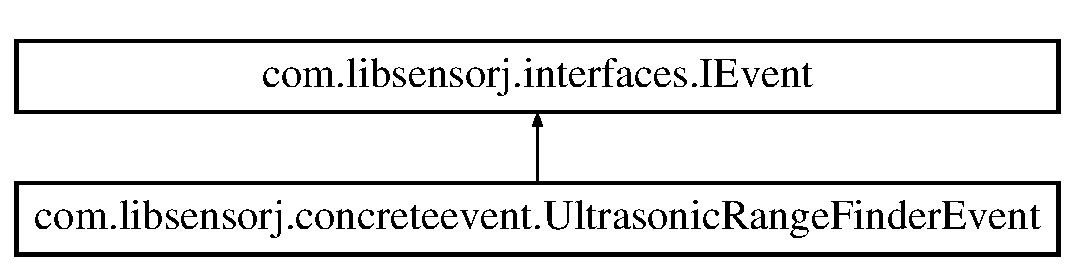
\includegraphics[height=2.000000cm]{classcom_1_1libsensorj_1_1concreteevent_1_1UltrasonicRangeFinderEvent}
\end{center}
\end{figure}
\subsection*{Public Member Functions}
\begin{DoxyCompactItemize}
\item 
void \hyperlink{classcom_1_1libsensorj_1_1concreteevent_1_1UltrasonicRangeFinderEvent_a0b32d3efeb55247269b4f43e4e34fe8e}{attach} (\hyperlink{classcom_1_1libsensorj_1_1model_1_1Observer}{Observer} obsever)
\item 
void \hyperlink{classcom_1_1libsensorj_1_1concreteevent_1_1UltrasonicRangeFinderEvent_ab0647f65e87ff07f61b3e4fe7e1daa19}{detach} (\hyperlink{classcom_1_1libsensorj_1_1model_1_1Observer}{Observer} obsever)
\item 
void \hyperlink{classcom_1_1libsensorj_1_1concreteevent_1_1UltrasonicRangeFinderEvent_a4d1ba316d1d324c4fb6e321e4c7a7b6e}{trigger} ()
\end{DoxyCompactItemize}


\subsection{Member Function Documentation}
\hypertarget{classcom_1_1libsensorj_1_1concreteevent_1_1UltrasonicRangeFinderEvent_a0b32d3efeb55247269b4f43e4e34fe8e}{}\index{com\+::libsensorj\+::concreteevent\+::\+Ultrasonic\+Range\+Finder\+Event@{com\+::libsensorj\+::concreteevent\+::\+Ultrasonic\+Range\+Finder\+Event}!attach@{attach}}
\index{attach@{attach}!com\+::libsensorj\+::concreteevent\+::\+Ultrasonic\+Range\+Finder\+Event@{com\+::libsensorj\+::concreteevent\+::\+Ultrasonic\+Range\+Finder\+Event}}
\subsubsection[{attach}]{\setlength{\rightskip}{0pt plus 5cm}void com.\+libsensorj.\+concreteevent.\+Ultrasonic\+Range\+Finder\+Event.\+attach (
\begin{DoxyParamCaption}
\item[{{\bf Observer}}]{obsever}
\end{DoxyParamCaption}
)}\label{classcom_1_1libsensorj_1_1concreteevent_1_1UltrasonicRangeFinderEvent_a0b32d3efeb55247269b4f43e4e34fe8e}


Implements \hyperlink{interfacecom_1_1libsensorj_1_1interfaces_1_1IEvent_af5af4301ccb6670452419d68baddf372}{com.\+libsensorj.\+interfaces.\+I\+Event}.

\hypertarget{classcom_1_1libsensorj_1_1concreteevent_1_1UltrasonicRangeFinderEvent_ab0647f65e87ff07f61b3e4fe7e1daa19}{}\index{com\+::libsensorj\+::concreteevent\+::\+Ultrasonic\+Range\+Finder\+Event@{com\+::libsensorj\+::concreteevent\+::\+Ultrasonic\+Range\+Finder\+Event}!detach@{detach}}
\index{detach@{detach}!com\+::libsensorj\+::concreteevent\+::\+Ultrasonic\+Range\+Finder\+Event@{com\+::libsensorj\+::concreteevent\+::\+Ultrasonic\+Range\+Finder\+Event}}
\subsubsection[{detach}]{\setlength{\rightskip}{0pt plus 5cm}void com.\+libsensorj.\+concreteevent.\+Ultrasonic\+Range\+Finder\+Event.\+detach (
\begin{DoxyParamCaption}
\item[{{\bf Observer}}]{obsever}
\end{DoxyParamCaption}
)}\label{classcom_1_1libsensorj_1_1concreteevent_1_1UltrasonicRangeFinderEvent_ab0647f65e87ff07f61b3e4fe7e1daa19}


Implements \hyperlink{interfacecom_1_1libsensorj_1_1interfaces_1_1IEvent_a974b07df97fda9f3be8e4afcd46470b2}{com.\+libsensorj.\+interfaces.\+I\+Event}.

\hypertarget{classcom_1_1libsensorj_1_1concreteevent_1_1UltrasonicRangeFinderEvent_a4d1ba316d1d324c4fb6e321e4c7a7b6e}{}\index{com\+::libsensorj\+::concreteevent\+::\+Ultrasonic\+Range\+Finder\+Event@{com\+::libsensorj\+::concreteevent\+::\+Ultrasonic\+Range\+Finder\+Event}!trigger@{trigger}}
\index{trigger@{trigger}!com\+::libsensorj\+::concreteevent\+::\+Ultrasonic\+Range\+Finder\+Event@{com\+::libsensorj\+::concreteevent\+::\+Ultrasonic\+Range\+Finder\+Event}}
\subsubsection[{trigger}]{\setlength{\rightskip}{0pt plus 5cm}void com.\+libsensorj.\+concreteevent.\+Ultrasonic\+Range\+Finder\+Event.\+trigger (
\begin{DoxyParamCaption}
{}
\end{DoxyParamCaption}
)}\label{classcom_1_1libsensorj_1_1concreteevent_1_1UltrasonicRangeFinderEvent_a4d1ba316d1d324c4fb6e321e4c7a7b6e}


Implements \hyperlink{interfacecom_1_1libsensorj_1_1interfaces_1_1IEvent_a861dea0956f77dd82f95e0110b8043b2}{com.\+libsensorj.\+interfaces.\+I\+Event}.



The documentation for this class was generated from the following file\+:\begin{DoxyCompactItemize}
\item 
main/java/com/libsensorj/concreteevent/\hyperlink{UltrasonicRangeFinderEvent_8java}{Ultrasonic\+Range\+Finder\+Event.\+java}\end{DoxyCompactItemize}

\hypertarget{classcom_1_1libsensorj_1_1examples_1_1UltrasonicRangeFinderExample}{}\section{com.\+libsensorj.\+examples.\+Ultrasonic\+Range\+Finder\+Example Class Reference}
\label{classcom_1_1libsensorj_1_1examples_1_1UltrasonicRangeFinderExample}\index{com.\+libsensorj.\+examples.\+Ultrasonic\+Range\+Finder\+Example@{com.\+libsensorj.\+examples.\+Ultrasonic\+Range\+Finder\+Example}}
\subsection*{Static Public Member Functions}
\begin{DoxyCompactItemize}
\item 
static void \hyperlink{classcom_1_1libsensorj_1_1examples_1_1UltrasonicRangeFinderExample_a587a298526337ce9e0d1fbbb9f400180}{main} (String\mbox{[}$\,$\mbox{]} args)
\end{DoxyCompactItemize}
\subsection*{Static Private Attributes}
\begin{DoxyCompactItemize}
\item 
static \hyperlink{interfacecom_1_1libsensorj_1_1interfaces_1_1ISensor}{I\+Sensor} \hyperlink{classcom_1_1libsensorj_1_1examples_1_1UltrasonicRangeFinderExample_af4703590c0c8bce89386204ea46afc76}{hcsr}
\item 
static final Logger \hyperlink{classcom_1_1libsensorj_1_1examples_1_1UltrasonicRangeFinderExample_ac1d433a89455addc211f404fe522f0ec}{L\+O\+G\+G\+E\+R}
\end{DoxyCompactItemize}


\subsection{Detailed Description}
The Class \hyperlink{classcom_1_1libsensorj_1_1examples_1_1UltrasonicRangeFinderExample}{Ultrasonic\+Range\+Finder\+Example}. 

\subsection{Member Function Documentation}
\hypertarget{classcom_1_1libsensorj_1_1examples_1_1UltrasonicRangeFinderExample_a587a298526337ce9e0d1fbbb9f400180}{}\index{com\+::libsensorj\+::examples\+::\+Ultrasonic\+Range\+Finder\+Example@{com\+::libsensorj\+::examples\+::\+Ultrasonic\+Range\+Finder\+Example}!main@{main}}
\index{main@{main}!com\+::libsensorj\+::examples\+::\+Ultrasonic\+Range\+Finder\+Example@{com\+::libsensorj\+::examples\+::\+Ultrasonic\+Range\+Finder\+Example}}
\subsubsection[{main}]{\setlength{\rightskip}{0pt plus 5cm}static void com.\+libsensorj.\+examples.\+Ultrasonic\+Range\+Finder\+Example.\+main (
\begin{DoxyParamCaption}
\item[{String\mbox{[}$\,$\mbox{]}}]{args}
\end{DoxyParamCaption}
)\hspace{0.3cm}{\ttfamily [static]}}\label{classcom_1_1libsensorj_1_1examples_1_1UltrasonicRangeFinderExample_a587a298526337ce9e0d1fbbb9f400180}
The main method.


\begin{DoxyParams}{Parameters}
{\em args} & the arguments \\
\hline
\end{DoxyParams}


\subsection{Member Data Documentation}
\hypertarget{classcom_1_1libsensorj_1_1examples_1_1UltrasonicRangeFinderExample_af4703590c0c8bce89386204ea46afc76}{}\index{com\+::libsensorj\+::examples\+::\+Ultrasonic\+Range\+Finder\+Example@{com\+::libsensorj\+::examples\+::\+Ultrasonic\+Range\+Finder\+Example}!hcsr@{hcsr}}
\index{hcsr@{hcsr}!com\+::libsensorj\+::examples\+::\+Ultrasonic\+Range\+Finder\+Example@{com\+::libsensorj\+::examples\+::\+Ultrasonic\+Range\+Finder\+Example}}
\subsubsection[{hcsr}]{\setlength{\rightskip}{0pt plus 5cm}{\bf I\+Sensor} com.\+libsensorj.\+examples.\+Ultrasonic\+Range\+Finder\+Example.\+hcsr\hspace{0.3cm}{\ttfamily [static]}, {\ttfamily [private]}}\label{classcom_1_1libsensorj_1_1examples_1_1UltrasonicRangeFinderExample_af4703590c0c8bce89386204ea46afc76}
The I\+Sensor hcsr. \hypertarget{classcom_1_1libsensorj_1_1examples_1_1UltrasonicRangeFinderExample_ac1d433a89455addc211f404fe522f0ec}{}\index{com\+::libsensorj\+::examples\+::\+Ultrasonic\+Range\+Finder\+Example@{com\+::libsensorj\+::examples\+::\+Ultrasonic\+Range\+Finder\+Example}!L\+O\+G\+G\+E\+R@{L\+O\+G\+G\+E\+R}}
\index{L\+O\+G\+G\+E\+R@{L\+O\+G\+G\+E\+R}!com\+::libsensorj\+::examples\+::\+Ultrasonic\+Range\+Finder\+Example@{com\+::libsensorj\+::examples\+::\+Ultrasonic\+Range\+Finder\+Example}}
\subsubsection[{L\+O\+G\+G\+E\+R}]{\setlength{\rightskip}{0pt plus 5cm}final Logger com.\+libsensorj.\+examples.\+Ultrasonic\+Range\+Finder\+Example.\+L\+O\+G\+G\+E\+R\hspace{0.3cm}{\ttfamily [static]}, {\ttfamily [private]}}\label{classcom_1_1libsensorj_1_1examples_1_1UltrasonicRangeFinderExample_ac1d433a89455addc211f404fe522f0ec}
{\bfseries Initial value\+:}
\begin{DoxyCode}
= LogManager
            .getLogger(UltrasonicRangeFinderExample.class.getName())
\end{DoxyCode}
The Constant L\+O\+G\+G\+E\+R. 

The documentation for this class was generated from the following file\+:\begin{DoxyCompactItemize}
\item 
main/java/com/libsensorj/examples/\hyperlink{UltrasonicRangeFinderExample_8java}{Ultrasonic\+Range\+Finder\+Example.\+java}\end{DoxyCompactItemize}

\hypertarget{classcom_1_1libsensorj_1_1concretefactory_1_1UltrasonicRangeFinderFactory}{}\section{com.\+libsensorj.\+concretefactory.\+Ultrasonic\+Range\+Finder\+Factory Class Reference}
\label{classcom_1_1libsensorj_1_1concretefactory_1_1UltrasonicRangeFinderFactory}\index{com.\+libsensorj.\+concretefactory.\+Ultrasonic\+Range\+Finder\+Factory@{com.\+libsensorj.\+concretefactory.\+Ultrasonic\+Range\+Finder\+Factory}}
Inheritance diagram for com.\+libsensorj.\+concretefactory.\+Ultrasonic\+Range\+Finder\+Factory\+:\begin{figure}[H]
\begin{center}
\leavevmode
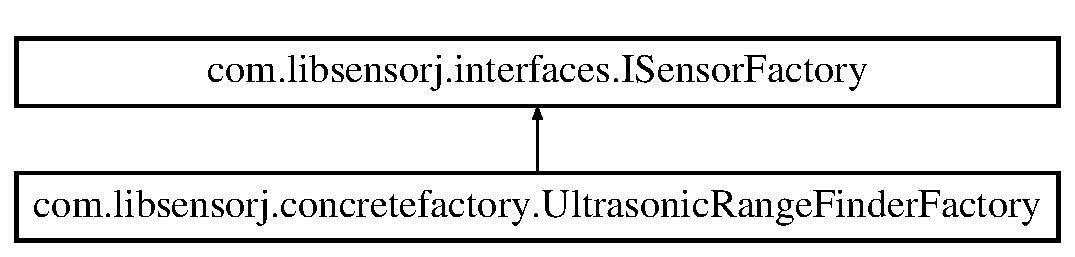
\includegraphics[height=2.000000cm]{classcom_1_1libsensorj_1_1concretefactory_1_1UltrasonicRangeFinderFactory}
\end{center}
\end{figure}
\subsection*{Public Member Functions}
\begin{DoxyCompactItemize}
\item 
\hyperlink{interfacecom_1_1libsensorj_1_1interfaces_1_1ISensor}{I\+Sensor} \hyperlink{classcom_1_1libsensorj_1_1concretefactory_1_1UltrasonicRangeFinderFactory_a3aa6e46ef47bf97355df4d5cfb1b1e01}{create\+Sensor} ()
\item 
\hyperlink{interfacecom_1_1libsensorj_1_1interfaces_1_1IEvent}{I\+Event} \hyperlink{classcom_1_1libsensorj_1_1concretefactory_1_1UltrasonicRangeFinderFactory_a8a7d0c55346f1ab5630a878f6a3175fd}{create\+Event} ()
\end{DoxyCompactItemize}


\subsection{Member Function Documentation}
\hypertarget{classcom_1_1libsensorj_1_1concretefactory_1_1UltrasonicRangeFinderFactory_a8a7d0c55346f1ab5630a878f6a3175fd}{}\index{com\+::libsensorj\+::concretefactory\+::\+Ultrasonic\+Range\+Finder\+Factory@{com\+::libsensorj\+::concretefactory\+::\+Ultrasonic\+Range\+Finder\+Factory}!create\+Event@{create\+Event}}
\index{create\+Event@{create\+Event}!com\+::libsensorj\+::concretefactory\+::\+Ultrasonic\+Range\+Finder\+Factory@{com\+::libsensorj\+::concretefactory\+::\+Ultrasonic\+Range\+Finder\+Factory}}
\subsubsection[{create\+Event}]{\setlength{\rightskip}{0pt plus 5cm}{\bf I\+Event} com.\+libsensorj.\+concretefactory.\+Ultrasonic\+Range\+Finder\+Factory.\+create\+Event (
\begin{DoxyParamCaption}
{}
\end{DoxyParamCaption}
)}\label{classcom_1_1libsensorj_1_1concretefactory_1_1UltrasonicRangeFinderFactory_a8a7d0c55346f1ab5630a878f6a3175fd}


Implements \hyperlink{interfacecom_1_1libsensorj_1_1interfaces_1_1ISensorFactory_a2b074d01287a4e64677097255ba9e768}{com.\+libsensorj.\+interfaces.\+I\+Sensor\+Factory}.

\hypertarget{classcom_1_1libsensorj_1_1concretefactory_1_1UltrasonicRangeFinderFactory_a3aa6e46ef47bf97355df4d5cfb1b1e01}{}\index{com\+::libsensorj\+::concretefactory\+::\+Ultrasonic\+Range\+Finder\+Factory@{com\+::libsensorj\+::concretefactory\+::\+Ultrasonic\+Range\+Finder\+Factory}!create\+Sensor@{create\+Sensor}}
\index{create\+Sensor@{create\+Sensor}!com\+::libsensorj\+::concretefactory\+::\+Ultrasonic\+Range\+Finder\+Factory@{com\+::libsensorj\+::concretefactory\+::\+Ultrasonic\+Range\+Finder\+Factory}}
\subsubsection[{create\+Sensor}]{\setlength{\rightskip}{0pt plus 5cm}{\bf I\+Sensor} com.\+libsensorj.\+concretefactory.\+Ultrasonic\+Range\+Finder\+Factory.\+create\+Sensor (
\begin{DoxyParamCaption}
{}
\end{DoxyParamCaption}
)}\label{classcom_1_1libsensorj_1_1concretefactory_1_1UltrasonicRangeFinderFactory_a3aa6e46ef47bf97355df4d5cfb1b1e01}


Implements \hyperlink{interfacecom_1_1libsensorj_1_1interfaces_1_1ISensorFactory_ac14c6d566c37c6a79c6db1e85634f25d}{com.\+libsensorj.\+interfaces.\+I\+Sensor\+Factory}.



The documentation for this class was generated from the following file\+:\begin{DoxyCompactItemize}
\item 
main/java/com/libsensorj/concretefactory/\hyperlink{UltrasonicRangeFinderFactory_8java}{Ultrasonic\+Range\+Finder\+Factory.\+java}\end{DoxyCompactItemize}

\chapter{File Documentation}
\hypertarget{IStepperMotor_8java}{}\section{main/java/com/libsensorj/concreteactuator/interfaces/\+I\+Stepper\+Motor.java File Reference}
\label{IStepperMotor_8java}\index{main/java/com/libsensorj/concreteactuator/interfaces/\+I\+Stepper\+Motor.\+java@{main/java/com/libsensorj/concreteactuator/interfaces/\+I\+Stepper\+Motor.\+java}}
\subsection*{Classes}
\begin{DoxyCompactItemize}
\item 
interface \hyperlink{interfacecom_1_1libsensorj_1_1concreteactuator_1_1interfaces_1_1IStepperMotor}{com.\+libsensorj.\+concreteactuator.\+interfaces.\+I\+Stepper\+Motor}
\end{DoxyCompactItemize}
\subsection*{Packages}
\begin{DoxyCompactItemize}
\item 
package \hyperlink{namespacecom_1_1libsensorj_1_1concreteactuator_1_1interfaces}{com.\+libsensorj.\+concreteactuator.\+interfaces}
\end{DoxyCompactItemize}

\hypertarget{StepperMotor_8java}{}\section{main/java/com/libsensorj/concreteactuator/\+Stepper\+Motor.java File Reference}
\label{StepperMotor_8java}\index{main/java/com/libsensorj/concreteactuator/\+Stepper\+Motor.\+java@{main/java/com/libsensorj/concreteactuator/\+Stepper\+Motor.\+java}}
\subsection*{Classes}
\begin{DoxyCompactItemize}
\item 
class \hyperlink{classcom_1_1libsensorj_1_1concreteactuator_1_1StepperMotor}{com.\+libsensorj.\+concreteactuator.\+Stepper\+Motor}
\item 
class \hyperlink{classcom_1_1libsensorj_1_1concreteactuator_1_1StepperMotor_1_1GpioStepperMotorControl}{com.\+libsensorj.\+concreteactuator.\+Stepper\+Motor.\+Gpio\+Stepper\+Motor\+Control}
\end{DoxyCompactItemize}
\subsection*{Packages}
\begin{DoxyCompactItemize}
\item 
package \hyperlink{namespacecom_1_1libsensorj_1_1concreteactuator}{com.\+libsensorj.\+concreteactuator}
\end{DoxyCompactItemize}

\hypertarget{HumidityEvent_8java}{}\section{main/java/com/libsensorj/concreteevent/\+Humidity\+Event.java File Reference}
\label{HumidityEvent_8java}\index{main/java/com/libsensorj/concreteevent/\+Humidity\+Event.\+java@{main/java/com/libsensorj/concreteevent/\+Humidity\+Event.\+java}}
\subsection*{Classes}
\begin{DoxyCompactItemize}
\item 
class \hyperlink{classcom_1_1libsensorj_1_1concreteevent_1_1HumidityEvent}{com.\+libsensorj.\+concreteevent.\+Humidity\+Event}
\end{DoxyCompactItemize}
\subsection*{Packages}
\begin{DoxyCompactItemize}
\item 
package \hyperlink{namespacecom_1_1libsensorj_1_1concreteevent}{com.\+libsensorj.\+concreteevent}
\end{DoxyCompactItemize}

\hypertarget{TemperatureEvent_8java}{}\section{main/java/com/libsensorj/concreteevent/\+Temperature\+Event.java File Reference}
\label{TemperatureEvent_8java}\index{main/java/com/libsensorj/concreteevent/\+Temperature\+Event.\+java@{main/java/com/libsensorj/concreteevent/\+Temperature\+Event.\+java}}
\subsection*{Classes}
\begin{DoxyCompactItemize}
\item 
class \hyperlink{classcom_1_1libsensorj_1_1concreteevent_1_1TemperatureEvent}{com.\+libsensorj.\+concreteevent.\+Temperature\+Event}
\end{DoxyCompactItemize}
\subsection*{Packages}
\begin{DoxyCompactItemize}
\item 
package \hyperlink{namespacecom_1_1libsensorj_1_1concreteevent}{com.\+libsensorj.\+concreteevent}
\end{DoxyCompactItemize}

\hypertarget{UltrasonicRangeFinderEvent_8java}{}\section{main/java/com/libsensorj/concreteevent/\+Ultrasonic\+Range\+Finder\+Event.java File Reference}
\label{UltrasonicRangeFinderEvent_8java}\index{main/java/com/libsensorj/concreteevent/\+Ultrasonic\+Range\+Finder\+Event.\+java@{main/java/com/libsensorj/concreteevent/\+Ultrasonic\+Range\+Finder\+Event.\+java}}
\subsection*{Classes}
\begin{DoxyCompactItemize}
\item 
class \hyperlink{classcom_1_1libsensorj_1_1concreteevent_1_1UltrasonicRangeFinderEvent}{com.\+libsensorj.\+concreteevent.\+Ultrasonic\+Range\+Finder\+Event}
\end{DoxyCompactItemize}
\subsection*{Packages}
\begin{DoxyCompactItemize}
\item 
package \hyperlink{namespacecom_1_1libsensorj_1_1concreteevent}{com.\+libsensorj.\+concreteevent}
\end{DoxyCompactItemize}

\hypertarget{DHT11V2Factory_8java}{}\section{main/java/com/libsensorj/concretefactory/\+D\+H\+T11\+V2\+Factory.java File Reference}
\label{DHT11V2Factory_8java}\index{main/java/com/libsensorj/concretefactory/\+D\+H\+T11\+V2\+Factory.\+java@{main/java/com/libsensorj/concretefactory/\+D\+H\+T11\+V2\+Factory.\+java}}
\subsection*{Classes}
\begin{DoxyCompactItemize}
\item 
class \hyperlink{classcom_1_1libsensorj_1_1concretefactory_1_1DHT11V2Factory}{com.\+libsensorj.\+concretefactory.\+D\+H\+T11\+V2\+Factory}
\end{DoxyCompactItemize}
\subsection*{Packages}
\begin{DoxyCompactItemize}
\item 
package \hyperlink{namespacecom_1_1libsensorj_1_1concretefactory}{com.\+libsensorj.\+concretefactory}
\end{DoxyCompactItemize}

\hypertarget{DHT11V3Factory_8java}{}\section{main/java/com/libsensorj/concretefactory/\+D\+H\+T11\+V3\+Factory.java File Reference}
\label{DHT11V3Factory_8java}\index{main/java/com/libsensorj/concretefactory/\+D\+H\+T11\+V3\+Factory.\+java@{main/java/com/libsensorj/concretefactory/\+D\+H\+T11\+V3\+Factory.\+java}}
\subsection*{Classes}
\begin{DoxyCompactItemize}
\item 
class \hyperlink{classcom_1_1libsensorj_1_1concretefactory_1_1DHT11V3Factory}{com.\+libsensorj.\+concretefactory.\+D\+H\+T11\+V3\+Factory}
\end{DoxyCompactItemize}
\subsection*{Packages}
\begin{DoxyCompactItemize}
\item 
package \hyperlink{namespacecom_1_1libsensorj_1_1concretefactory}{com.\+libsensorj.\+concretefactory}
\end{DoxyCompactItemize}

\hypertarget{HCSR04DeviceFactory_8java}{}\section{main/java/com/libsensorj/concretefactory/\+H\+C\+S\+R04\+Device\+Factory.java File Reference}
\label{HCSR04DeviceFactory_8java}\index{main/java/com/libsensorj/concretefactory/\+H\+C\+S\+R04\+Device\+Factory.\+java@{main/java/com/libsensorj/concretefactory/\+H\+C\+S\+R04\+Device\+Factory.\+java}}
\subsection*{Classes}
\begin{DoxyCompactItemize}
\item 
class \hyperlink{classcom_1_1libsensorj_1_1concretefactory_1_1HCSR04DeviceFactory}{com.\+libsensorj.\+concretefactory.\+H\+C\+S\+R04\+Device\+Factory}
\end{DoxyCompactItemize}
\subsection*{Packages}
\begin{DoxyCompactItemize}
\item 
package \hyperlink{namespacecom_1_1libsensorj_1_1concretefactory}{com.\+libsensorj.\+concretefactory}
\end{DoxyCompactItemize}

\hypertarget{HumiditySensorFactory_8java}{}\section{main/java/com/libsensorj/concretefactory/\+Humidity\+Sensor\+Factory.java File Reference}
\label{HumiditySensorFactory_8java}\index{main/java/com/libsensorj/concretefactory/\+Humidity\+Sensor\+Factory.\+java@{main/java/com/libsensorj/concretefactory/\+Humidity\+Sensor\+Factory.\+java}}
\subsection*{Classes}
\begin{DoxyCompactItemize}
\item 
class \hyperlink{classcom_1_1libsensorj_1_1concretefactory_1_1HumiditySensorFactory}{com.\+libsensorj.\+concretefactory.\+Humidity\+Sensor\+Factory}
\end{DoxyCompactItemize}
\subsection*{Packages}
\begin{DoxyCompactItemize}
\item 
package \hyperlink{namespacecom_1_1libsensorj_1_1concretefactory}{com.\+libsensorj.\+concretefactory}
\end{DoxyCompactItemize}

\hypertarget{RotaryEncoderFactory_8java}{}\section{main/java/com/libsensorj/concretefactory/\+Rotary\+Encoder\+Factory.java File Reference}
\label{RotaryEncoderFactory_8java}\index{main/java/com/libsensorj/concretefactory/\+Rotary\+Encoder\+Factory.\+java@{main/java/com/libsensorj/concretefactory/\+Rotary\+Encoder\+Factory.\+java}}
\subsection*{Classes}
\begin{DoxyCompactItemize}
\item 
class \hyperlink{classcom_1_1libsensorj_1_1concretefactory_1_1RotaryEncoderFactory}{com.\+libsensorj.\+concretefactory.\+Rotary\+Encoder\+Factory}
\end{DoxyCompactItemize}
\subsection*{Packages}
\begin{DoxyCompactItemize}
\item 
package \hyperlink{namespacecom_1_1libsensorj_1_1concretefactory}{com.\+libsensorj.\+concretefactory}
\end{DoxyCompactItemize}

\hypertarget{TemperatureSensorFactory_8java}{}\section{main/java/com/libsensorj/concretefactory/\+Temperature\+Sensor\+Factory.java File Reference}
\label{TemperatureSensorFactory_8java}\index{main/java/com/libsensorj/concretefactory/\+Temperature\+Sensor\+Factory.\+java@{main/java/com/libsensorj/concretefactory/\+Temperature\+Sensor\+Factory.\+java}}
\subsection*{Classes}
\begin{DoxyCompactItemize}
\item 
class \hyperlink{classcom_1_1libsensorj_1_1concretefactory_1_1TemperatureSensorFactory}{com.\+libsensorj.\+concretefactory.\+Temperature\+Sensor\+Factory}
\end{DoxyCompactItemize}
\subsection*{Packages}
\begin{DoxyCompactItemize}
\item 
package \hyperlink{namespacecom_1_1libsensorj_1_1concretefactory}{com.\+libsensorj.\+concretefactory}
\end{DoxyCompactItemize}

\hypertarget{UltrasonicRangeFinderFactory_8java}{}\section{main/java/com/libsensorj/concretefactory/\+Ultrasonic\+Range\+Finder\+Factory.java File Reference}
\label{UltrasonicRangeFinderFactory_8java}\index{main/java/com/libsensorj/concretefactory/\+Ultrasonic\+Range\+Finder\+Factory.\+java@{main/java/com/libsensorj/concretefactory/\+Ultrasonic\+Range\+Finder\+Factory.\+java}}
\subsection*{Classes}
\begin{DoxyCompactItemize}
\item 
class \hyperlink{classcom_1_1libsensorj_1_1concretefactory_1_1UltrasonicRangeFinderFactory}{com.\+libsensorj.\+concretefactory.\+Ultrasonic\+Range\+Finder\+Factory}
\end{DoxyCompactItemize}
\subsection*{Packages}
\begin{DoxyCompactItemize}
\item 
package \hyperlink{namespacecom_1_1libsensorj_1_1concretefactory}{com.\+libsensorj.\+concretefactory}
\end{DoxyCompactItemize}

\hypertarget{DHT11_8java}{}\section{main/java/com/libsensorj/concretesensor/\+D\+H\+T11.java File Reference}
\label{DHT11_8java}\index{main/java/com/libsensorj/concretesensor/\+D\+H\+T11.\+java@{main/java/com/libsensorj/concretesensor/\+D\+H\+T11.\+java}}
\subsection*{Classes}
\begin{DoxyCompactItemize}
\item 
class \hyperlink{classcom_1_1libsensorj_1_1concretesensor_1_1DHT11}{com.\+libsensorj.\+concretesensor.\+D\+H\+T11}
\end{DoxyCompactItemize}
\subsection*{Packages}
\begin{DoxyCompactItemize}
\item 
package \hyperlink{namespacecom_1_1libsensorj_1_1concretesensor}{com.\+libsensorj.\+concretesensor}
\end{DoxyCompactItemize}

\hypertarget{DHT11Humidity_8java}{}\section{main/java/com/libsensorj/concretesensor/\+D\+H\+T11\+Humidity.java File Reference}
\label{DHT11Humidity_8java}\index{main/java/com/libsensorj/concretesensor/\+D\+H\+T11\+Humidity.\+java@{main/java/com/libsensorj/concretesensor/\+D\+H\+T11\+Humidity.\+java}}
\subsection*{Classes}
\begin{DoxyCompactItemize}
\item 
class \hyperlink{classcom_1_1libsensorj_1_1concretesensor_1_1DHT11Humidity}{com.\+libsensorj.\+concretesensor.\+D\+H\+T11\+Humidity}
\end{DoxyCompactItemize}
\subsection*{Packages}
\begin{DoxyCompactItemize}
\item 
package \hyperlink{namespacecom_1_1libsensorj_1_1concretesensor}{com.\+libsensorj.\+concretesensor}
\end{DoxyCompactItemize}

\hypertarget{DHT11Temperature_8java}{}\section{main/java/com/libsensorj/concretesensor/\+D\+H\+T11\+Temperature.java File Reference}
\label{DHT11Temperature_8java}\index{main/java/com/libsensorj/concretesensor/\+D\+H\+T11\+Temperature.\+java@{main/java/com/libsensorj/concretesensor/\+D\+H\+T11\+Temperature.\+java}}
\subsection*{Classes}
\begin{DoxyCompactItemize}
\item 
class \hyperlink{classcom_1_1libsensorj_1_1concretesensor_1_1DHT11Temperature}{com.\+libsensorj.\+concretesensor.\+D\+H\+T11\+Temperature}
\end{DoxyCompactItemize}
\subsection*{Packages}
\begin{DoxyCompactItemize}
\item 
package \hyperlink{namespacecom_1_1libsensorj_1_1concretesensor}{com.\+libsensorj.\+concretesensor}
\end{DoxyCompactItemize}

\hypertarget{DHT11V2_8java}{}\section{main/java/com/libsensorj/concretesensor/\+D\+H\+T11\+V2.java File Reference}
\label{DHT11V2_8java}\index{main/java/com/libsensorj/concretesensor/\+D\+H\+T11\+V2.\+java@{main/java/com/libsensorj/concretesensor/\+D\+H\+T11\+V2.\+java}}
\subsection*{Classes}
\begin{DoxyCompactItemize}
\item 
class \hyperlink{classcom_1_1libsensorj_1_1concretesensor_1_1DHT11V2}{com.\+libsensorj.\+concretesensor.\+D\+H\+T11\+V2}
\end{DoxyCompactItemize}
\subsection*{Packages}
\begin{DoxyCompactItemize}
\item 
package \hyperlink{namespacecom_1_1libsensorj_1_1concretesensor}{com.\+libsensorj.\+concretesensor}
\end{DoxyCompactItemize}

\hypertarget{DHT11V3_8java}{}\section{main/java/com/libsensorj/concretesensor/\+D\+H\+T11\+V3.java File Reference}
\label{DHT11V3_8java}\index{main/java/com/libsensorj/concretesensor/\+D\+H\+T11\+V3.\+java@{main/java/com/libsensorj/concretesensor/\+D\+H\+T11\+V3.\+java}}
\subsection*{Classes}
\begin{DoxyCompactItemize}
\item 
class \hyperlink{classcom_1_1libsensorj_1_1concretesensor_1_1DHT11V3}{com.\+libsensorj.\+concretesensor.\+D\+H\+T11\+V3}
\end{DoxyCompactItemize}
\subsection*{Packages}
\begin{DoxyCompactItemize}
\item 
package \hyperlink{namespacecom_1_1libsensorj_1_1concretesensor}{com.\+libsensorj.\+concretesensor}
\end{DoxyCompactItemize}

\hypertarget{HCSR04Device_8java}{}\section{main/java/com/libsensorj/concretesensor/\+H\+C\+S\+R04\+Device.java File Reference}
\label{HCSR04Device_8java}\index{main/java/com/libsensorj/concretesensor/\+H\+C\+S\+R04\+Device.\+java@{main/java/com/libsensorj/concretesensor/\+H\+C\+S\+R04\+Device.\+java}}
\subsection*{Classes}
\begin{DoxyCompactItemize}
\item 
class \hyperlink{classcom_1_1libsensorj_1_1concretesensor_1_1HCSR04Device}{com.\+libsensorj.\+concretesensor.\+H\+C\+S\+R04\+Device}
\end{DoxyCompactItemize}
\subsection*{Packages}
\begin{DoxyCompactItemize}
\item 
package \hyperlink{namespacecom_1_1libsensorj_1_1concretesensor}{com.\+libsensorj.\+concretesensor}
\end{DoxyCompactItemize}

\hypertarget{HCSR04V2_8java}{}\section{main/java/com/libsensorj/concretesensor/\+H\+C\+S\+R04\+V2.java File Reference}
\label{HCSR04V2_8java}\index{main/java/com/libsensorj/concretesensor/\+H\+C\+S\+R04\+V2.\+java@{main/java/com/libsensorj/concretesensor/\+H\+C\+S\+R04\+V2.\+java}}
\subsection*{Classes}
\begin{DoxyCompactItemize}
\item 
class \hyperlink{classcom_1_1libsensorj_1_1concretesensor_1_1HCSR04V2}{com.\+libsensorj.\+concretesensor.\+H\+C\+S\+R04\+V2}
\end{DoxyCompactItemize}
\subsection*{Packages}
\begin{DoxyCompactItemize}
\item 
package \hyperlink{namespacecom_1_1libsensorj_1_1concretesensor}{com.\+libsensorj.\+concretesensor}
\end{DoxyCompactItemize}

\hypertarget{HCSR04V3_8java}{}\section{main/java/com/libsensorj/concretesensor/\+H\+C\+S\+R04\+V3.java File Reference}
\label{HCSR04V3_8java}\index{main/java/com/libsensorj/concretesensor/\+H\+C\+S\+R04\+V3.\+java@{main/java/com/libsensorj/concretesensor/\+H\+C\+S\+R04\+V3.\+java}}
\subsection*{Classes}
\begin{DoxyCompactItemize}
\item 
class \hyperlink{classcom_1_1libsensorj_1_1concretesensor_1_1HCSR04V3}{com.\+libsensorj.\+concretesensor.\+H\+C\+S\+R04\+V3}
\end{DoxyCompactItemize}
\subsection*{Packages}
\begin{DoxyCompactItemize}
\item 
package \hyperlink{namespacecom_1_1libsensorj_1_1concretesensor}{com.\+libsensorj.\+concretesensor}
\end{DoxyCompactItemize}

\hypertarget{RotaryEncoder_8java}{}\section{main/java/com/libsensorj/concretesensor/\+Rotary\+Encoder.java File Reference}
\label{RotaryEncoder_8java}\index{main/java/com/libsensorj/concretesensor/\+Rotary\+Encoder.\+java@{main/java/com/libsensorj/concretesensor/\+Rotary\+Encoder.\+java}}
\subsection*{Classes}
\begin{DoxyCompactItemize}
\item 
class \hyperlink{classcom_1_1libsensorj_1_1concretesensor_1_1RotaryEncoder}{com.\+libsensorj.\+concretesensor.\+Rotary\+Encoder}
\end{DoxyCompactItemize}
\subsection*{Packages}
\begin{DoxyCompactItemize}
\item 
package \hyperlink{namespacecom_1_1libsensorj_1_1concretesensor}{com.\+libsensorj.\+concretesensor}
\end{DoxyCompactItemize}

\hypertarget{UltrasonicHcsr04_8java}{}\section{main/java/com/libsensorj/concretesensor/\+Ultrasonic\+Hcsr04.java File Reference}
\label{UltrasonicHcsr04_8java}\index{main/java/com/libsensorj/concretesensor/\+Ultrasonic\+Hcsr04.\+java@{main/java/com/libsensorj/concretesensor/\+Ultrasonic\+Hcsr04.\+java}}
\subsection*{Classes}
\begin{DoxyCompactItemize}
\item 
class \hyperlink{classcom_1_1libsensorj_1_1concretesensor_1_1UltrasonicHcsr04}{com.\+libsensorj.\+concretesensor.\+Ultrasonic\+Hcsr04}
\end{DoxyCompactItemize}
\subsection*{Packages}
\begin{DoxyCompactItemize}
\item 
package \hyperlink{namespacecom_1_1libsensorj_1_1concretesensor}{com.\+libsensorj.\+concretesensor}
\end{DoxyCompactItemize}

\hypertarget{DHT11HumidityExample_8java}{}\section{main/java/com/libsensorj/examples/\+D\+H\+T11\+Humidity\+Example.java File Reference}
\label{DHT11HumidityExample_8java}\index{main/java/com/libsensorj/examples/\+D\+H\+T11\+Humidity\+Example.\+java@{main/java/com/libsensorj/examples/\+D\+H\+T11\+Humidity\+Example.\+java}}
\subsection*{Classes}
\begin{DoxyCompactItemize}
\item 
class \hyperlink{classcom_1_1libsensorj_1_1examples_1_1DHT11HumidityExample}{com.\+libsensorj.\+examples.\+D\+H\+T11\+Humidity\+Example}
\end{DoxyCompactItemize}
\subsection*{Packages}
\begin{DoxyCompactItemize}
\item 
package \hyperlink{namespacecom_1_1libsensorj_1_1examples}{com.\+libsensorj.\+examples}
\end{DoxyCompactItemize}

\hypertarget{DHT11TemperatureExample_8java}{}\section{main/java/com/libsensorj/examples/\+D\+H\+T11\+Temperature\+Example.java File Reference}
\label{DHT11TemperatureExample_8java}\index{main/java/com/libsensorj/examples/\+D\+H\+T11\+Temperature\+Example.\+java@{main/java/com/libsensorj/examples/\+D\+H\+T11\+Temperature\+Example.\+java}}
\subsection*{Classes}
\begin{DoxyCompactItemize}
\item 
class \hyperlink{classcom_1_1libsensorj_1_1examples_1_1DHT11TemperatureExample}{com.\+libsensorj.\+examples.\+D\+H\+T11\+Temperature\+Example}
\end{DoxyCompactItemize}
\subsection*{Packages}
\begin{DoxyCompactItemize}
\item 
package \hyperlink{namespacecom_1_1libsensorj_1_1examples}{com.\+libsensorj.\+examples}
\end{DoxyCompactItemize}

\hypertarget{DHT11V2Example_8java}{}\section{main/java/com/libsensorj/examples/\+D\+H\+T11\+V2\+Example.java File Reference}
\label{DHT11V2Example_8java}\index{main/java/com/libsensorj/examples/\+D\+H\+T11\+V2\+Example.\+java@{main/java/com/libsensorj/examples/\+D\+H\+T11\+V2\+Example.\+java}}
\subsection*{Classes}
\begin{DoxyCompactItemize}
\item 
class \hyperlink{classcom_1_1libsensorj_1_1examples_1_1DHT11V2Example}{com.\+libsensorj.\+examples.\+D\+H\+T11\+V2\+Example}
\end{DoxyCompactItemize}
\subsection*{Packages}
\begin{DoxyCompactItemize}
\item 
package \hyperlink{namespacecom_1_1libsensorj_1_1examples}{com.\+libsensorj.\+examples}
\end{DoxyCompactItemize}

\hypertarget{DHT11V3Example_8java}{}\section{main/java/com/libsensorj/examples/\+D\+H\+T11\+V3\+Example.java File Reference}
\label{DHT11V3Example_8java}\index{main/java/com/libsensorj/examples/\+D\+H\+T11\+V3\+Example.\+java@{main/java/com/libsensorj/examples/\+D\+H\+T11\+V3\+Example.\+java}}
\subsection*{Classes}
\begin{DoxyCompactItemize}
\item 
class \hyperlink{classcom_1_1libsensorj_1_1examples_1_1DHT11V3Example}{com.\+libsensorj.\+examples.\+D\+H\+T11\+V3\+Example}
\end{DoxyCompactItemize}
\subsection*{Packages}
\begin{DoxyCompactItemize}
\item 
package \hyperlink{namespacecom_1_1libsensorj_1_1examples}{com.\+libsensorj.\+examples}
\end{DoxyCompactItemize}

\hypertarget{HCSR04DeviceExample_8java}{}\section{main/java/com/libsensorj/examples/\+H\+C\+S\+R04\+Device\+Example.java File Reference}
\label{HCSR04DeviceExample_8java}\index{main/java/com/libsensorj/examples/\+H\+C\+S\+R04\+Device\+Example.\+java@{main/java/com/libsensorj/examples/\+H\+C\+S\+R04\+Device\+Example.\+java}}
\subsection*{Classes}
\begin{DoxyCompactItemize}
\item 
class \hyperlink{classcom_1_1libsensorj_1_1examples_1_1HCSR04DeviceExample}{com.\+libsensorj.\+examples.\+H\+C\+S\+R04\+Device\+Example}
\end{DoxyCompactItemize}
\subsection*{Packages}
\begin{DoxyCompactItemize}
\item 
package \hyperlink{namespacecom_1_1libsensorj_1_1examples}{com.\+libsensorj.\+examples}
\end{DoxyCompactItemize}

\hypertarget{HCSR04NoSensorClass_8java}{}\section{main/java/com/libsensorj/examples/\+H\+C\+S\+R04\+No\+Sensor\+Class.java File Reference}
\label{HCSR04NoSensorClass_8java}\index{main/java/com/libsensorj/examples/\+H\+C\+S\+R04\+No\+Sensor\+Class.\+java@{main/java/com/libsensorj/examples/\+H\+C\+S\+R04\+No\+Sensor\+Class.\+java}}
\subsection*{Classes}
\begin{DoxyCompactItemize}
\item 
class \hyperlink{classcom_1_1libsensorj_1_1examples_1_1HCSR04NoSensorClass}{com.\+libsensorj.\+examples.\+H\+C\+S\+R04\+No\+Sensor\+Class}
\end{DoxyCompactItemize}
\subsection*{Packages}
\begin{DoxyCompactItemize}
\item 
package \hyperlink{namespacecom_1_1libsensorj_1_1examples}{com.\+libsensorj.\+examples}
\end{DoxyCompactItemize}

\hypertarget{HCSR04V2Example_8java}{}\section{main/java/com/libsensorj/examples/\+H\+C\+S\+R04\+V2\+Example.java File Reference}
\label{HCSR04V2Example_8java}\index{main/java/com/libsensorj/examples/\+H\+C\+S\+R04\+V2\+Example.\+java@{main/java/com/libsensorj/examples/\+H\+C\+S\+R04\+V2\+Example.\+java}}
\subsection*{Classes}
\begin{DoxyCompactItemize}
\item 
class \hyperlink{classcom_1_1libsensorj_1_1examples_1_1HCSR04V2Example}{com.\+libsensorj.\+examples.\+H\+C\+S\+R04\+V2\+Example}
\end{DoxyCompactItemize}
\subsection*{Packages}
\begin{DoxyCompactItemize}
\item 
package \hyperlink{namespacecom_1_1libsensorj_1_1examples}{com.\+libsensorj.\+examples}
\end{DoxyCompactItemize}

\hypertarget{HCSR04V3Example_8java}{}\section{main/java/com/libsensorj/examples/\+H\+C\+S\+R04\+V3\+Example.java File Reference}
\label{HCSR04V3Example_8java}\index{main/java/com/libsensorj/examples/\+H\+C\+S\+R04\+V3\+Example.\+java@{main/java/com/libsensorj/examples/\+H\+C\+S\+R04\+V3\+Example.\+java}}
\subsection*{Classes}
\begin{DoxyCompactItemize}
\item 
class \hyperlink{classcom_1_1libsensorj_1_1examples_1_1HCSR04V3Example}{com.\+libsensorj.\+examples.\+H\+C\+S\+R04\+V3\+Example}
\end{DoxyCompactItemize}
\subsection*{Packages}
\begin{DoxyCompactItemize}
\item 
package \hyperlink{namespacecom_1_1libsensorj_1_1examples}{com.\+libsensorj.\+examples}
\end{DoxyCompactItemize}

\hypertarget{StepperMotorExample_8java}{}\section{main/java/com/libsensorj/examples/\+Stepper\+Motor\+Example.java File Reference}
\label{StepperMotorExample_8java}\index{main/java/com/libsensorj/examples/\+Stepper\+Motor\+Example.\+java@{main/java/com/libsensorj/examples/\+Stepper\+Motor\+Example.\+java}}
\subsection*{Classes}
\begin{DoxyCompactItemize}
\item 
class \hyperlink{classcom_1_1libsensorj_1_1examples_1_1StepperMotorExample}{com.\+libsensorj.\+examples.\+Stepper\+Motor\+Example}
\end{DoxyCompactItemize}
\subsection*{Packages}
\begin{DoxyCompactItemize}
\item 
package \hyperlink{namespacecom_1_1libsensorj_1_1examples}{com.\+libsensorj.\+examples}
\end{DoxyCompactItemize}

\hypertarget{UltrasonicRangeFinderExample_8java}{}\section{main/java/com/libsensorj/examples/\+Ultrasonic\+Range\+Finder\+Example.java File Reference}
\label{UltrasonicRangeFinderExample_8java}\index{main/java/com/libsensorj/examples/\+Ultrasonic\+Range\+Finder\+Example.\+java@{main/java/com/libsensorj/examples/\+Ultrasonic\+Range\+Finder\+Example.\+java}}
\subsection*{Classes}
\begin{DoxyCompactItemize}
\item 
class \hyperlink{classcom_1_1libsensorj_1_1examples_1_1UltrasonicRangeFinderExample}{com.\+libsensorj.\+examples.\+Ultrasonic\+Range\+Finder\+Example}
\end{DoxyCompactItemize}
\subsection*{Packages}
\begin{DoxyCompactItemize}
\item 
package \hyperlink{namespacecom_1_1libsensorj_1_1examples}{com.\+libsensorj.\+examples}
\end{DoxyCompactItemize}

\hypertarget{IActuator_8java}{}\section{main/java/com/libsensorj/interfaces/\+I\+Actuator.java File Reference}
\label{IActuator_8java}\index{main/java/com/libsensorj/interfaces/\+I\+Actuator.\+java@{main/java/com/libsensorj/interfaces/\+I\+Actuator.\+java}}
\subsection*{Classes}
\begin{DoxyCompactItemize}
\item 
interface \hyperlink{interfacecom_1_1libsensorj_1_1interfaces_1_1IActuator}{com.\+libsensorj.\+interfaces.\+I\+Actuator}
\end{DoxyCompactItemize}
\subsection*{Packages}
\begin{DoxyCompactItemize}
\item 
package \hyperlink{namespacecom_1_1libsensorj_1_1interfaces}{com.\+libsensorj.\+interfaces}
\end{DoxyCompactItemize}

\hypertarget{IEvent_8java}{}\section{main/java/com/libsensorj/interfaces/\+I\+Event.java File Reference}
\label{IEvent_8java}\index{main/java/com/libsensorj/interfaces/\+I\+Event.\+java@{main/java/com/libsensorj/interfaces/\+I\+Event.\+java}}
\subsection*{Classes}
\begin{DoxyCompactItemize}
\item 
interface \hyperlink{interfacecom_1_1libsensorj_1_1interfaces_1_1IEvent}{com.\+libsensorj.\+interfaces.\+I\+Event}
\end{DoxyCompactItemize}
\subsection*{Packages}
\begin{DoxyCompactItemize}
\item 
package \hyperlink{namespacecom_1_1libsensorj_1_1interfaces}{com.\+libsensorj.\+interfaces}
\end{DoxyCompactItemize}

\hypertarget{ISensor_8java}{}\section{main/java/com/libsensorj/interfaces/\+I\+Sensor.java File Reference}
\label{ISensor_8java}\index{main/java/com/libsensorj/interfaces/\+I\+Sensor.\+java@{main/java/com/libsensorj/interfaces/\+I\+Sensor.\+java}}
\subsection*{Classes}
\begin{DoxyCompactItemize}
\item 
interface \hyperlink{interfacecom_1_1libsensorj_1_1interfaces_1_1ISensor}{com.\+libsensorj.\+interfaces.\+I\+Sensor}
\end{DoxyCompactItemize}
\subsection*{Packages}
\begin{DoxyCompactItemize}
\item 
package \hyperlink{namespacecom_1_1libsensorj_1_1interfaces}{com.\+libsensorj.\+interfaces}
\end{DoxyCompactItemize}

\hypertarget{ISensorFactory_8java}{}\section{main/java/com/libsensorj/interfaces/\+I\+Sensor\+Factory.java File Reference}
\label{ISensorFactory_8java}\index{main/java/com/libsensorj/interfaces/\+I\+Sensor\+Factory.\+java@{main/java/com/libsensorj/interfaces/\+I\+Sensor\+Factory.\+java}}
\subsection*{Classes}
\begin{DoxyCompactItemize}
\item 
interface \hyperlink{interfacecom_1_1libsensorj_1_1interfaces_1_1ISensorFactory}{com.\+libsensorj.\+interfaces.\+I\+Sensor\+Factory}
\end{DoxyCompactItemize}
\subsection*{Packages}
\begin{DoxyCompactItemize}
\item 
package \hyperlink{namespacecom_1_1libsensorj_1_1interfaces}{com.\+libsensorj.\+interfaces}
\end{DoxyCompactItemize}

\hypertarget{RotaryEncoderListener_8java}{}\section{main/java/com/libsensorj/listeners/\+Rotary\+Encoder\+Listener.java File Reference}
\label{RotaryEncoderListener_8java}\index{main/java/com/libsensorj/listeners/\+Rotary\+Encoder\+Listener.\+java@{main/java/com/libsensorj/listeners/\+Rotary\+Encoder\+Listener.\+java}}
\subsection*{Classes}
\begin{DoxyCompactItemize}
\item 
interface \hyperlink{interfacecom_1_1libsensorj_1_1listeners_1_1RotaryEncoderListener}{com.\+libsensorj.\+listeners.\+Rotary\+Encoder\+Listener}
\end{DoxyCompactItemize}
\subsection*{Packages}
\begin{DoxyCompactItemize}
\item 
package \hyperlink{namespacecom_1_1libsensorj_1_1listeners}{com.\+libsensorj.\+listeners}
\end{DoxyCompactItemize}

\hypertarget{RotaryEncoderListenerImpl_8java}{}\section{main/java/com/libsensorj/listeners/\+Rotary\+Encoder\+Listener\+Impl.java File Reference}
\label{RotaryEncoderListenerImpl_8java}\index{main/java/com/libsensorj/listeners/\+Rotary\+Encoder\+Listener\+Impl.\+java@{main/java/com/libsensorj/listeners/\+Rotary\+Encoder\+Listener\+Impl.\+java}}
\subsection*{Classes}
\begin{DoxyCompactItemize}
\item 
class \hyperlink{classcom_1_1libsensorj_1_1listeners_1_1RotaryEncoderListenerImpl}{com.\+libsensorj.\+listeners.\+Rotary\+Encoder\+Listener\+Impl}
\end{DoxyCompactItemize}
\subsection*{Packages}
\begin{DoxyCompactItemize}
\item 
package \hyperlink{namespacecom_1_1libsensorj_1_1listeners}{com.\+libsensorj.\+listeners}
\end{DoxyCompactItemize}

\hypertarget{Observer_8java}{}\section{main/java/com/libsensorj/model/\+Observer.java File Reference}
\label{Observer_8java}\index{main/java/com/libsensorj/model/\+Observer.\+java@{main/java/com/libsensorj/model/\+Observer.\+java}}
\subsection*{Classes}
\begin{DoxyCompactItemize}
\item 
class \hyperlink{classcom_1_1libsensorj_1_1model_1_1Observer}{com.\+libsensorj.\+model.\+Observer}
\end{DoxyCompactItemize}
\subsection*{Packages}
\begin{DoxyCompactItemize}
\item 
package \hyperlink{namespacecom_1_1libsensorj_1_1model}{com.\+libsensorj.\+model}
\end{DoxyCompactItemize}

\hypertarget{LibPins_8java}{}\section{main/java/com/libsensorj/utils/\+Lib\+Pins.java File Reference}
\label{LibPins_8java}\index{main/java/com/libsensorj/utils/\+Lib\+Pins.\+java@{main/java/com/libsensorj/utils/\+Lib\+Pins.\+java}}
\subsection*{Classes}
\begin{DoxyCompactItemize}
\item 
class \hyperlink{classcom_1_1libsensorj_1_1utils_1_1LibPins}{com.\+libsensorj.\+utils.\+Lib\+Pins}
\end{DoxyCompactItemize}
\subsection*{Packages}
\begin{DoxyCompactItemize}
\item 
package \hyperlink{namespacecom_1_1libsensorj_1_1utils}{com.\+libsensorj.\+utils}
\end{DoxyCompactItemize}

\hypertarget{PinNumbers_8java}{}\section{main/java/com/libsensorj/utils/\+Pin\+Numbers.java File Reference}
\label{PinNumbers_8java}\index{main/java/com/libsensorj/utils/\+Pin\+Numbers.\+java@{main/java/com/libsensorj/utils/\+Pin\+Numbers.\+java}}
\subsection*{Classes}
\begin{DoxyCompactItemize}
\item 
enum \hyperlink{enumcom_1_1libsensorj_1_1utils_1_1PinNumbers}{com.\+libsensorj.\+utils.\+Pin\+Numbers}
\end{DoxyCompactItemize}
\subsection*{Packages}
\begin{DoxyCompactItemize}
\item 
package \hyperlink{namespacecom_1_1libsensorj_1_1utils}{com.\+libsensorj.\+utils}
\end{DoxyCompactItemize}

\hypertarget{MyExample_8java}{}\section{main/java/com/pi4j/examples/\+My\+Example.java File Reference}
\label{MyExample_8java}\index{main/java/com/pi4j/examples/\+My\+Example.\+java@{main/java/com/pi4j/examples/\+My\+Example.\+java}}
\subsection*{Classes}
\begin{DoxyCompactItemize}
\item 
class \hyperlink{classcom_1_1pi4j_1_1examples_1_1MyExample}{com.\+pi4j.\+examples.\+My\+Example}
\end{DoxyCompactItemize}
\subsection*{Packages}
\begin{DoxyCompactItemize}
\item 
package \hyperlink{namespacecom_1_1pi4j_1_1examples}{com.\+pi4j.\+examples}
\end{DoxyCompactItemize}

\hypertarget{TemperatureSensorFactoryTests_8java}{}\section{test/java/com/libsensorj/concretefactory/test/\+Temperature\+Sensor\+Factory\+Tests.java File Reference}
\label{TemperatureSensorFactoryTests_8java}\index{test/java/com/libsensorj/concretefactory/test/\+Temperature\+Sensor\+Factory\+Tests.\+java@{test/java/com/libsensorj/concretefactory/test/\+Temperature\+Sensor\+Factory\+Tests.\+java}}
\subsection*{Classes}
\begin{DoxyCompactItemize}
\item 
class \hyperlink{classcom_1_1libsensorj_1_1concretefactory_1_1test_1_1TemperatureSensorFactoryTests}{com.\+libsensorj.\+concretefactory.\+test.\+Temperature\+Sensor\+Factory\+Tests}
\end{DoxyCompactItemize}
\subsection*{Packages}
\begin{DoxyCompactItemize}
\item 
package \hyperlink{namespacecom_1_1libsensorj_1_1concretefactory_1_1test}{com.\+libsensorj.\+concretefactory.\+test}
\end{DoxyCompactItemize}

\hypertarget{DHT11HumidityTests_8java}{}\section{test/java/com/libsensorj/concretesensor/test/\+D\+H\+T11\+Humidity\+Tests.java File Reference}
\label{DHT11HumidityTests_8java}\index{test/java/com/libsensorj/concretesensor/test/\+D\+H\+T11\+Humidity\+Tests.\+java@{test/java/com/libsensorj/concretesensor/test/\+D\+H\+T11\+Humidity\+Tests.\+java}}
\subsection*{Classes}
\begin{DoxyCompactItemize}
\item 
class \hyperlink{classcom_1_1libsensorj_1_1concretesensor_1_1test_1_1DHT11HumidityTests}{com.\+libsensorj.\+concretesensor.\+test.\+D\+H\+T11\+Humidity\+Tests}
\end{DoxyCompactItemize}
\subsection*{Packages}
\begin{DoxyCompactItemize}
\item 
package \hyperlink{namespacecom_1_1libsensorj_1_1concretesensor_1_1test}{com.\+libsensorj.\+concretesensor.\+test}
\end{DoxyCompactItemize}

\hypertarget{DHT11TemperatureTests_8java}{}\section{test/java/com/libsensorj/concretesensor/test/\+D\+H\+T11\+Temperature\+Tests.java File Reference}
\label{DHT11TemperatureTests_8java}\index{test/java/com/libsensorj/concretesensor/test/\+D\+H\+T11\+Temperature\+Tests.\+java@{test/java/com/libsensorj/concretesensor/test/\+D\+H\+T11\+Temperature\+Tests.\+java}}
\subsection*{Classes}
\begin{DoxyCompactItemize}
\item 
class \hyperlink{classcom_1_1libsensorj_1_1concretesensor_1_1test_1_1DHT11TemperatureTests}{com.\+libsensorj.\+concretesensor.\+test.\+D\+H\+T11\+Temperature\+Tests}
\end{DoxyCompactItemize}
\subsection*{Packages}
\begin{DoxyCompactItemize}
\item 
package \hyperlink{namespacecom_1_1libsensorj_1_1concretesensor_1_1test}{com.\+libsensorj.\+concretesensor.\+test}
\end{DoxyCompactItemize}

\hypertarget{DHT11V2Tests_8java}{}\section{test/java/com/libsensorj/concretesensor/test/\+D\+H\+T11\+V2\+Tests.java File Reference}
\label{DHT11V2Tests_8java}\index{test/java/com/libsensorj/concretesensor/test/\+D\+H\+T11\+V2\+Tests.\+java@{test/java/com/libsensorj/concretesensor/test/\+D\+H\+T11\+V2\+Tests.\+java}}
\subsection*{Classes}
\begin{DoxyCompactItemize}
\item 
class \hyperlink{classcom_1_1libsensorj_1_1concretesensor_1_1test_1_1DHT11V2Tests}{com.\+libsensorj.\+concretesensor.\+test.\+D\+H\+T11\+V2\+Tests}
\end{DoxyCompactItemize}
\subsection*{Packages}
\begin{DoxyCompactItemize}
\item 
package \hyperlink{namespacecom_1_1libsensorj_1_1concretesensor_1_1test}{com.\+libsensorj.\+concretesensor.\+test}
\end{DoxyCompactItemize}

\hypertarget{DHT11V3Tests_8java}{}\section{test/java/com/libsensorj/concretesensor/test/\+D\+H\+T11\+V3\+Tests.java File Reference}
\label{DHT11V3Tests_8java}\index{test/java/com/libsensorj/concretesensor/test/\+D\+H\+T11\+V3\+Tests.\+java@{test/java/com/libsensorj/concretesensor/test/\+D\+H\+T11\+V3\+Tests.\+java}}
\subsection*{Classes}
\begin{DoxyCompactItemize}
\item 
class \hyperlink{classcom_1_1libsensorj_1_1concretesensor_1_1test_1_1DHT11V3Tests}{com.\+libsensorj.\+concretesensor.\+test.\+D\+H\+T11\+V3\+Tests}
\end{DoxyCompactItemize}
\subsection*{Packages}
\begin{DoxyCompactItemize}
\item 
package \hyperlink{namespacecom_1_1libsensorj_1_1concretesensor_1_1test}{com.\+libsensorj.\+concretesensor.\+test}
\end{DoxyCompactItemize}

\hypertarget{HCSR04DeviceTests_8java}{}\section{test/java/com/libsensorj/concretesensor/test/\+H\+C\+S\+R04\+Device\+Tests.java File Reference}
\label{HCSR04DeviceTests_8java}\index{test/java/com/libsensorj/concretesensor/test/\+H\+C\+S\+R04\+Device\+Tests.\+java@{test/java/com/libsensorj/concretesensor/test/\+H\+C\+S\+R04\+Device\+Tests.\+java}}
\subsection*{Classes}
\begin{DoxyCompactItemize}
\item 
class \hyperlink{classcom_1_1libsensorj_1_1concretesensor_1_1test_1_1HCSR04DeviceTests}{com.\+libsensorj.\+concretesensor.\+test.\+H\+C\+S\+R04\+Device\+Tests}
\end{DoxyCompactItemize}
\subsection*{Packages}
\begin{DoxyCompactItemize}
\item 
package \hyperlink{namespacecom_1_1libsensorj_1_1concretesensor_1_1test}{com.\+libsensorj.\+concretesensor.\+test}
\end{DoxyCompactItemize}

\hypertarget{UltrasonicHcsr04Tests_8java}{}\section{test/java/com/libsensorj/concretesensor/test/\+Ultrasonic\+Hcsr04\+Tests.java File Reference}
\label{UltrasonicHcsr04Tests_8java}\index{test/java/com/libsensorj/concretesensor/test/\+Ultrasonic\+Hcsr04\+Tests.\+java@{test/java/com/libsensorj/concretesensor/test/\+Ultrasonic\+Hcsr04\+Tests.\+java}}
\subsection*{Classes}
\begin{DoxyCompactItemize}
\item 
class \hyperlink{classcom_1_1libsensorj_1_1concretesensor_1_1test_1_1UltrasonicHcsr04Tests}{com.\+libsensorj.\+concretesensor.\+test.\+Ultrasonic\+Hcsr04\+Tests}
\end{DoxyCompactItemize}
\subsection*{Packages}
\begin{DoxyCompactItemize}
\item 
package \hyperlink{namespacecom_1_1libsensorj_1_1concretesensor_1_1test}{com.\+libsensorj.\+concretesensor.\+test}
\end{DoxyCompactItemize}

\hypertarget{MockGpioFactory_8java}{}\section{test/java/com/libsensorj/mock/\+Mock\+Gpio\+Factory.java File Reference}
\label{MockGpioFactory_8java}\index{test/java/com/libsensorj/mock/\+Mock\+Gpio\+Factory.\+java@{test/java/com/libsensorj/mock/\+Mock\+Gpio\+Factory.\+java}}
\subsection*{Classes}
\begin{DoxyCompactItemize}
\item 
class \hyperlink{classcom_1_1libsensorj_1_1mock_1_1MockGpioFactory}{com.\+libsensorj.\+mock.\+Mock\+Gpio\+Factory}
\end{DoxyCompactItemize}
\subsection*{Packages}
\begin{DoxyCompactItemize}
\item 
package \hyperlink{namespacecom_1_1libsensorj_1_1mock}{com.\+libsensorj.\+mock}
\end{DoxyCompactItemize}

\hypertarget{MockGpioProvider_8java}{}\section{test/java/com/libsensorj/mock/\+Mock\+Gpio\+Provider.java File Reference}
\label{MockGpioProvider_8java}\index{test/java/com/libsensorj/mock/\+Mock\+Gpio\+Provider.\+java@{test/java/com/libsensorj/mock/\+Mock\+Gpio\+Provider.\+java}}
\subsection*{Classes}
\begin{DoxyCompactItemize}
\item 
class \hyperlink{classcom_1_1libsensorj_1_1mock_1_1MockGpioProvider}{com.\+libsensorj.\+mock.\+Mock\+Gpio\+Provider}
\end{DoxyCompactItemize}
\subsection*{Packages}
\begin{DoxyCompactItemize}
\item 
package \hyperlink{namespacecom_1_1libsensorj_1_1mock}{com.\+libsensorj.\+mock}
\end{DoxyCompactItemize}

\hypertarget{MockPin_8java}{}\section{test/java/com/libsensorj/mock/\+Mock\+Pin.java File Reference}
\label{MockPin_8java}\index{test/java/com/libsensorj/mock/\+Mock\+Pin.\+java@{test/java/com/libsensorj/mock/\+Mock\+Pin.\+java}}
\subsection*{Classes}
\begin{DoxyCompactItemize}
\item 
class \hyperlink{classcom_1_1libsensorj_1_1mock_1_1MockPin}{com.\+libsensorj.\+mock.\+Mock\+Pin}
\end{DoxyCompactItemize}
\subsection*{Packages}
\begin{DoxyCompactItemize}
\item 
package \hyperlink{namespacecom_1_1libsensorj_1_1mock}{com.\+libsensorj.\+mock}
\end{DoxyCompactItemize}

\hypertarget{HelloTests_8java}{}\section{test/java/test\+Hello/\+Hello\+Tests.java File Reference}
\label{HelloTests_8java}\index{test/java/test\+Hello/\+Hello\+Tests.\+java@{test/java/test\+Hello/\+Hello\+Tests.\+java}}
\subsection*{Classes}
\begin{DoxyCompactItemize}
\item 
class \hyperlink{classtestHello_1_1HelloTests}{test\+Hello.\+Hello\+Tests}
\end{DoxyCompactItemize}
\subsection*{Packages}
\begin{DoxyCompactItemize}
\item 
package \hyperlink{namespacetestHello}{test\+Hello}
\end{DoxyCompactItemize}

%--- End generated contents ---

% Index
\backmatter
\newpage
\phantomsection
\clearemptydoublepage
\addcontentsline{toc}{chapter}{Index}
\printindex

\end{document}
